\documentclass[a4paper,12pt,oneside]{article}

\usepackage[utf8]{inputenc}
\usepackage[T1,T2A]{fontenc}
\usepackage[english,russian]{babel}
\usepackage[usenames]{xcolor}
\usepackage{etoolbox}
\usepackage{listings}
\usepackage{graphicx}
\usepackage{cmap}
\usepackage{indentfirst}
\usepackage{imakeidx}
\usepackage[unicode]{hyperref}

\newif\ifanswers
\answerstrue

\overfullrule=2cm
\righthyphenmin=2

\hypersetup{
%bookmarks=true,            % show bookmarks bar?
%unicode=false,             % non-Latin characters in Acrobat’s bookmarks
pdfproducer={Producer},    % producer of the document
pdfkeywords={keywords},    % list of keywords
pdfnewwindow=true,         % links in new window
colorlinks=true,           % false: boxed links; true: colored links
linkcolor=black,           % color of internal links
citecolor=black,           % color of links to bibliography
    filecolor=black,           % color of file links
    urlcolor=black             % color of external links
}

\renewcommand{\rmdefault}{cmr} 

\renewcommand{\texttt}[2][black]{\textcolor{#1}{\ttfamily #2}}

\definecolor{OliveGreen}{cmyk}{0.64,0,0.95,0.40}
\definecolor{mauve}{rgb}{0.58,0,0.82}

\setlength{\parskip}{6pt}

\makeindex[intoc]

\title{Лекции по C++}
\author{
  Владимиров Константин Игоревич\\
  \texttt{konstantin.vladimirov@gmail.com}
}
\date{\today}

\begin{document}

\begin{titlepage}
\begin{center}

\large ~ \\[4.5cm]

\huge Курс лекций\\[0.6cm]
\large По языку программирования C++\\[3.7cm]

\begin{minipage}{0.5\textwidth} % начало маленькой врезки в половину ширины текста
\begin{flushleft} % выровнять её содержимое по левому краю
\emph{Автор:} Владимиров К. И.\\
\end{flushleft} % конец выравнивания по левому краю
\end{minipage} % конец врезки

\vfill

Страница с последней редакцией: \url{sourceforge.net/projects/cpp-lects-rus}\\
Email автора: \texttt{konstantin.vladimirov@gmail.com}\\
{\large \today}
{\large \LaTeX}

\end{center}
\thispagestyle{empty}
\end{titlepage}

\tableofcontents

\lstset{
language=C++,                           % Code langugage
basicstyle=\ttfamily,                   % Code font, Examples: \footnotesize, \ttfamily
keywordstyle=\color{OliveGreen},        % Keywords font ('*' = uppercase)
commentstyle=\color{gray},              % Comments font
stringstyle=\color{mauve},
numbers=left,                           % Line nums position
numberstyle=\tiny,
numbersep=10pt,
stepnumber=1,                           % Step between two line-numbers
frame=none,                             % A frame around the code
tabsize=2,                              % Default tab size
captionpos=b,                           % Caption-position = bottom
breaklines=true,                        % Automatic line breaking?
breakatwhitespace=false,                % Automatic breaks only at whitespace?
showspaces=false,                       % Dont make spaces visible
showstringspaces=false,
showtabs=false,                         % Dont make tabls visible
columns=flexible,                       % Column format
title=\lstname,
caption={},
extendedchars=\true,
inputencoding=utf8,
}

\pagebreak
\section*{Программа курса}
\addcontentsline{toc}{section}{Программа курса}

\textbf{Первый семестр}

\begin{enumerate}
\item [Лекция 1.] Основные языковые конструкции в C и C++
\item [Лекция 2.] Введение в стандарт языка C++
\item [Лекция 3.] Переход от приемов C к приемам C++ 
\item [Лекция 4.] Препроцессор и базовые шаблоны функций
\item [Лекция 5.] Автоматический вывод типов
\item [Лекция 6.] Введение в ООП: инкапсуляция, конкретные классы
\item [Лекция 7.] Переопределение операторов
\item [Лекция 8.] RAII, семантика копирования и присваивания
\item [Лекция 9.] Rvalue ссылки и семантика перемещения
\item [Лекция 10.] Полиморфизм и наследование интерфейса
\item [Лекция 11.] Наследование реализации
\item [Лекция 12.] Множественное наследование и RTTI 
\item [Лекция 13.] Принципы ООП и паттерны проектирования 
\item [Лекция 14.] Шаблоны классов, часть 1: Специализация
\item [Лекция 15.] Шаблоны классов, часть 2: Шаблоны и ООП. CRTP.
\end{enumerate}

\textbf{Второй семестр}

\begin{enumerate}
\item [Лекция 16.] Исключения, часть 1: Генерация и обработка. Гарантии.
\item [Лекция 17.] Исключения, часть 2: Идиома PImpl
\item [Лекция 18.] Введение в стандартную библиотеку: последовательные контейнеры 
\item [Лекция 19.] Итераторы 
\item [Лекция 20.] Ассоциативные контейнеры 
\item [Лекция 21.] Ввод и вывод 
\item [Лекция 22.] Алгоритмы, часть 1: Немодифицирующие алгоритмы
\item [Лекция 23.] Алгоритмы, часть 2: Модифицирующие алгоритмы
\item [Лекция 24.] Вариабельные шаблоны
\item [Лекция 25.] Лямбда-выражения, часть 1: Замыкания
\item [Лекция 26.] Лямбда-выражения, часть 2: Монады
\item [Лекция 27.] Шаблоны классов, часть 3: SFINAE 
\item [Лекция 28.] Метапрограммирование на шаблонах 
\item [Лекция 29.] Вычисления времени компиляции, constexpr функции
\item [Лекция 30.] Общий обзор курса
\end{enumerate}

\pagebreak
\section{Общие сведения}\label{StdIntroduction}

C++ (произносится ``си плас плас'')\index{C++} это язык общего назначения с сильной статической типизацией и ручным управлением ресурсами. Де-факто в современном программировании C++ является индустриальным стандартом. Язык был создан Бьярном Строструпом\index{Stroustrup} в 1980-м году как объектно-ориентированное расширение языка C\index{C}, известного с 70-х. В 1985-м появилась первая коммерческая версия компилятора Cfront\index{Cfront} и по языку была опубликована первая книга. 

По прошествии времени, C++ был принят сообществом, широко распространился. Код на C++ переносимо работает на различных архитектурах и операционных системах. В 1998-м году язык C++ был стандартизован (работа велась с 1990-го года). Сейчас язык C++ имеет развитую инфраструктуру средств компиляции, отладки, библиотек, поддержку в IDE. Много новых возможностей было добавлено в язык очередным стандартом, принятым в 2011-м году. Ещё больше возможностей добавлено в стандарте, принятом в 2014-м году. В настоящее время ведется работа над стандартом, принятие которого запланировано на 2017-й год.

\subsection{Стандартизация C++}\label{Standartization}

\hfill\textit{First, I'd like to see the basic tools such as compilers,}

\hfill\textit{debuggers, profilers, database interfaces, GUI builders,} 

\hfill\textit{CAD tools, and so forth fully support the ISO standard}{\vspace{0.5em}}

\hfill\textit{-- Bjarne Stroustrup}

\textbf{Вопрос к студентам:} что такое ISO\index{ISO standard}, какие стандарты ISO вы знаете (читали).

Международная организация по стандартизации (ISO\index{ISO}) создана в 1946 году двадцатью пятью национальными организациями по стандартизации. На сегодняшний день в состав ИСО входит 165 стран. СССР был одним из основателей организации, постоянным членом руководящих органов, дважды представитель Госстандарта избирался председателем организации. Россия стала членом ИСО как правопреемник СССР. С 2005 года Россия входит в Совет ИСО. Официальными языками являются: английский, французский и русский. Конкретные стандарты могут быть опубликованы на одном из этих языков, но не обязательно на всех. Например, стандарт C++ опубликован только на английском языке.

Первый стандарт языка C++ под кодовым номером ISO/IEC 14882-1998 \cite{stdcpp98} был написан и утверждён ISO в 1998 году. Он включает в себя по нормативной ссылке стандарт языка C, ISO/IEC 9899-1990 \cite{stdc90}, что означает следующее: 

\begin{itemize}
\item
Возможности C90 (кроме явно оговоренных исключений) также являются возможностями C++98, также и стандартная библиотека языка C в ревизии C90 является стандартной библиотекой C++98
\item
Новые возможности C99 \cite{stdc90} не являются возможностями C++98 (стоит отметить, что стандарт C99 включён по ссылке в C++11 \cite{stdcpp11}, но стандарт C11 \cite{stdc11} снова разошёлся с текущим нижележащим подмножеством C в C++), снова был включен по нормативной ссылке в C++14 \cite{stdcpp14}
\end{itemize}

Текущий стандарт C++ имеет кодовый номер ISO/IEC 14882-2014

Важно знать какой стандарт по умолчанию поддерживает тот компилятор которым вы пользуетесь (и та его версия, которой вы пользуетесь в настоящий момент). Очень часто по умолчанию компилятор поддерживает не чистый стандарт (особенно в случае языка C) а стандарт с несколькими специфичными для конкретного компилятора расширениями. Скажем GCC 5.1 по умолчанию поддерживает для языка C стандарт C11 + GNU extensions (так называемый gnu11), а для языка C++ стандарт C++98 + GNU extensions (так называемый gnu++98).

Очень часто компиляторы поддерживают даже будущий стандарт. Типичный случай -- опция c++1z в GCC включает совместимость со всеми утвержденными на данный момент предложениями в ещё не принятый документ.

\textbf{Домашняя наработка:} посмотрите какой стандарт по умолчанию поддерживает ваш компилятор

\subsubsection{Важность стандартизации}\label{StandartizationImportance}

Стандарты и даже ошибки в стандартах отлиты в граните. Например, в стандарте IEEE POSIX 1003.1-1988 была допущена ошибка: в одной главе было указано, что \lstinline!PATH_MAX! включает terminating null, в то время, как в другой главе было указано что не включает. Ошибка была обнаружена после публикации стандарта, люди обратились в комиссию стандартизации и оттуда пришло объяснение, что если написано и так и так, значит может быть и так и так. Хотя изначально идея была как раз в том, чтобы определённо установить включает ли \lstinline!PATH_MAX! нулевой символ.

Язык как соглашение между программистами и разработчиками компиляторов утверждается своим стандартом и не существует вне его. Все стандарты ISO доступны бесплатно в версии final draft – последнего черновика перед утверждением. Часто пиратски доступны и окончательные версии.

Читать и понимать стандарт языка – то, чем занимается каждый программист при решении любых спорных вопросов, возникающих у него относительно тех или иных языковых средств. Это последняя и окончательная инстанция.

В качестве примера, вы пишете следующий код на чем-то, что кажется вам языком программирования C:

\lstinputlisting{cpp_code/p0-inline.c}

\textbf{Вопрос к студентам:} видите ли вы какие-нибудь проблемы в этом коде?

\ifanswers
Правильный ответ: проблемы есть. Этот код скомпилируется на GCC 4.9 и не скомпилируется на GCC 5.1 с опциями по умолчанию (проверьте, скомпилируется ли он на вашем любимом компиляторе).
\fi

Объяснение: изменение в стандарте C99 семантики \lstinline!inline! по сравнению с C++98 делает упомянутую тут \lstinline!extern inline! функцию необязательной заглушкой, которую компилятор имеет право выбросить. Подробности последуют в (\ref{Inline}).

И это только незначительный пример, который не приводит к особенно разрушительным последствиям и причины которого гуглятся сравнительно просто. Но по незнанию или ориентируясь на ``здравый смысл'' можно допустить существенно более серьезные просчеты. Все эти лекции можно считать приглашением к самостоятельной проработке стандарта C++ совместно с решением практических задач. Собственно, чтобы научится писать программы, надо знать язык и писать программы, иных вариантов нет.

Очень часто в этом конспекте будут делаться ссылки на пункты стандартов. Чтобы не путать их с главами, внутри круглых скобок будет ссылка на документ стандарта в списке литературы. Поэтому (5.1.2) это ссылка на главу 5.1.2 этого текста, тогда как (С11 5.1.2) это ссылка на пункт 5.1.2 стандарта C11 (\cite{stdc11}).

\subsubsection{Конформный код}\label{ConformingCode}

Стандарт языка C++ традиционно отличается от стандарта языка C тем, что стандарт C определяет корректность программы, написанной на C, стандарт же C++ определяет корректность компилятора. Это различие с первого раза кажется несущественным и бюрократическим, но во многом из-за него, например, стандарт C99 довольно долгое время не был целиком реализован ни в одном компиляторе C (и только недавно стал стандартом по умолчанию для GCC), поскольку конформные программы можно писать и с подмножеством возможностей. В то же время гораздо более сложный C++98 был реализован в некоторых компиляторах даже в своих наиболее эзотерических частях, таких как экспорт шаблонов.

Тем не менее, очень часто бывает проще даже в случае C++ кода говорить именно о качестве кода, поскольку программа это то, что (до определенной степени) можно модифицировать.

Любой код, подаваемый на вход удовлетворяющего стандарту компилятора, принадлежит к одной из следующих категорий:

\begin{itemize}
\item \textbf{Syntax violation}\index{Syntax violation} -- нечто, вообще не являющееся кодом на языке C++. Это наиболее распространённый вид кода, производимого программистами.

\item \textbf{Implementation defined}\index{Implementation defined} -- зависящий от разработчика и документации конкретного компилятора. Пример -- как ведёт себя знаковое целое при сдвиге вправо.

\item \textbf{Unspecified}\index{Unspecified} -- поведение корректного кода, не регламентированное стандартом. Пример -- порядок выполнения аргументов у функции.

\item \textbf{Undefined behavior}\index{Undefined behavior} -- поведение некорректного кода, не запрещённое стандартом. Пример – поведение знакового целого числа при переполнении.

\item \textbf{Strictly conforming}\index{Strictly conforming} -- отличный код, полностью удовлетворяющий стандарту и не выходящий за пределы стандарта. Редко встречается in anima vili и никогда у новичков.

\item \textbf{Conforming}\index{Conforming} -- код удовлетворяющий стандарту + использующий implementation defined features.
\end{itemize}

У разных компиляторов есть своя стратегия выдачи диагностических сообщений. Для компиляции большинства примеров из этих лекций, будет использован компилятор g++ версии 5.2.0 или выше, входящий в GNU Compiler Collection. Рекомендуемые опции: 

\lstinline!g++ -pedantic-errors -Wall -Werror -g3 -O0 --std=c++98!

\lstinline!g++ -pedantic-errors -Wall -Werror -g3 -O0 --std=c++14!

Эти опции заставляют репортить о не-conforming коде и воспринимать все диагностические сообщения как ошибки, а также включать отладочную информацию включая отладку по макросам и отключать все оптимизации (с моей точки зрения это единственный приемлимый способ компиляции учебных примеров).

Пример conforming кода на C-подмножестве C++:

\lstinputlisting{cpp_code/p0s1.cpp}

Приведённый выше код является conforming но не strictly conforming из-за использования \lstinline!INT_MAX!, являющегося implementation-defined. Тем не менее, нет способа заставить GCC выдать такое диагностическое предупреждение и этот код проходит компиляцию без ошибок, так что можно считать уровень conforming достаточным.

\pagebreak
\subsection{Неопределенное поведение}\label{UB}

Изо всех рассмотренных выше видов поведения программы, самое страшное это неопределённое поведение (undefined behavior, UB). Обратите внимание: аббревиатура UB здесь и далее употребляется только для undefined behavior, но никогда для unspecified, хотя там сокращение такое же.

Неопределённое поведение \textbf{не является злом:} отказ определять поведение в граничных ситуациях даёт компилятору возможность генерировать гораздо более оптимальный код. Иногда программист закладывает логический аналог неопределенного поведения в свою программу сознательно Например при удалении односвязного списка вы можете сказать, что поведение процедуры удаления не определено если в списке есть петля и именно это ограничение позволит написать удаление эффективно. Аналогично и стандарт каждым своим UB-clause оставляет компилятору свободу для маневра.

Тем не менее, UB является опасностью. Любой программист на языках C и C++ с некоторым опытом развивает чутьё на неопределённые ситуации, но даже профессионалы часто попадают в ловушки. В этих лекциях я предпочитаю остановиться на этой теме с самого начала, поскольку упомянутое выше чутьё надо развивать сразу. Сначала эффектный пример.

\subsubsection{Неявное UB как путь к проклятию}\label{HiddenUB}

Следующий код на C (взят из SPEC benchmark) выглядит достаточно невинно

\begin{lstlisting}
int k, satd = 0, dd, d[16];

/* ... more code here ... */

for (dd = d[k = 0]; k < 16; dd = d[++k])
  satd += (dd < 0 ? -dd : dd);
\end{lstlisting}

Но в эксперименте с GCC 4.8.0 получается бесконечный цикл. Компилятор на этапе agressive-loop-optimizations, считает, что без выхода за границы массива \lstinline!dd! не может быть больше 15. А раз 15 < 16, то и выход по условию \lstinline!dd < 16! невозможен, так что его и проверять не стоит.

Этот пример показателен тем, что в случае UB компилятор может не только \textbf{сделать} всё что угодно (например отформатировать диск), но и \textbf{не сделать} чего-то, причём компилятор даже не обязан об этом сообщать.

\subsubsection{Типичные случаи неопределённого поведения}\label{TypicalUB}

Здесь будет рассмотрен только язык C и C-подмножество C++. Проблемы, возникающие при работе с ООП и шаблонами будут рассмотрены в конце соответствующих частей. Типичными случаями неопределённого поведения являются:

\begin {itemize}
\item \textbf {Арифметика}
\begin {itemize}
\item Целочисленное знаковое переполнение
\item Математическая неопределенность результата (скажем целочисленное деление на 0)
\item Сдвиг влево на отрицательные значения
\item Сдвиг на значения, превышающие размер типа
\item Приведение целого числа к не вмещающему его типу
\item Попытка изменить константный объект, приведя его к не константному
\end {itemize}
\item \textbf {Указатели}
\begin {itemize}
\item Разыменование нулевого указателя
\item Разыменование неинициализированного указателя
\item Разыменование указателя на память, динамически выделенную с нулевым размером
\item Использование указателей и ссылок на объекты с истекшим сроком жизни
\item Адресная арифметика с результатом, выходящим за границы массива и доступ к такой памяти
\item Преобразование указателей в несовместимые типы
\item Использование memcpy на пересекающихся участках памяти
\end {itemize}
\item \textbf {Препроцессор}
\begin {itemize}
\item Непустой исходный файл, не оканчивающийся на пустую строку (или оканчивающийся на обратный слеш)
\item Обратный слеш после которого стоит нечто отличное от перечня escape-кодов
\item Выход за реализационные пределы (скажем 1024 условия в switch)
\item Динамически генерируемый токен под \lstinline!#if!
\end {itemize}
\end {itemize}

Разумеется этот список не претендует на полноту, но он даёт представление о местах, которых стоит опасаться.

\subsubsection{Пример исправления ситуации}\label{CorrectingUB}

Очень часто код, демонстрирующий неопределённое поведение, можно переписать на эквивалентный детерминированный. Это работает не во всех случаях, но гораздо чаще, чем многие думают. Типичный грозящий UB код:

\begin{lstlisting}
int foo(int a) 
{
  assert(a + 100 > a); /* ORLY? */
  printf("%d %d\n", a + 100, a);
  return a;
}
\end{lstlisting}

Автор этого кода скорее всего считает, что оградился от случаев арифметического знакового переполнения. На самом деле он просто заложился на неопределенное поведение. Простое переписывание кода сделает его гораздо более безопасным:

\begin{lstlisting}
int foo(int a) 
{
  assert(a < (INT_MAX - 100));
  printf("%d %d\n", a + 100, a);
  return a;
}
\end{lstlisting}

Если исправление ситуации с неопределённым поведением в ваших силах -- делайте это. Увы, иногда обнаружение неопределенного поведения на этапе компиляции проблематично:

\begin{lstlisting}
int foo(int* a, int len) 
{
  assert ((a != NULL) && (len > 1));
  return a[len/2];    /* ORLY? */
}
\end{lstlisting}

В случае если в \lstinline!len! передано неверное значение, здесь возможен выход за границы массива, который на этапе компиляции отловить сложно или невозможно. И здесь вступают в игру проверки времени исполнения -- так называемые санитайзеры.

\subsubsection{Поиск UB с помощью санитайзеров}\label{SanitizerUsage}

Некоторые компиляторы (такие как GCC) поддерживают инструментирование кода в местах, где возможно неопределенное поведение. Для GCC доступен вызов с опцией \lstinline!-fsanitize=undefined!, которая включает UndefinedBehaviorSanitizer -- open-source средство определения неопределенного поведения во время исполнения. Он проверяет почти все случаи рассмотренные в (\ref{TypicalUB}), но существенно замедляет программу, так как по сути генерирует вызов проверяющей функции на каждое знаковое суммирование, доступ по указателю, сдвиг и прочее.

Для того, чтобы проверить конкретный случай UB а не все их сразу, можно подать вместо undefined, одну из её подопций:

\begin{lstlisting}
-fsanitize=shift
-fsanitize=integer-divide-by-zero
-fsanitize=unreachable
-fsanitize=vla-bound
-fsanitize=null
-fsanitize=return
-fsanitize=signed-integer-overflow
-fsanitize=bounds
-fsanitize=bounds-strict
-fsanitize=alignment
-fsanitize=object-size
-fsanitize=float-divide-by-zero
-fsanitize=float-cast-overflow
-fsanitize=nonnull-attribute
-fsanitize=returns-nonnull-attribute
-fsanitize=bool
-fsanitize=enum
-fsanitize=vptr
\end{lstlisting}

Сама библиотека UBsan, поддерживающая всю эту функциональность перекочевала в GCC из LLVM/Clang поэтому доступна и там.

Очень полезно прогонять ваши программы под санитайзерами на предмет поиска сложных случаев UB которые вы не всегда сможете проверить глазами.

\textbf{Домашняя наработка:} попробуйте под санитайзером следующую программу на языке C:

\begin{lstlisting}
#include <stdlib.h>

int a = 0xecfb39f5;
unsigned short *d = (unsigned short *) &a;

int
main (void)
{
  if ((unsigned long) (65536 * d[1] + d[0]) < (1UL << 28))
    abort ();

  return 0;
}
\end{lstlisting}\label{lst:HWUB}

Демонстрирует ли она неопределенное поведение? Если да, то где? Предложите как исправить ситуацию.

\subsubsection{Статическая верификация кода}

\hfill\textit{Beware of bugs in the above code;}

\hfill\textit{I have only proved it correct, not tried it}{\vspace{0.5em}}

\hfill\textit{-- Donald E. Knuth}

Санитайзеры хороши, но у них есть проблема в некоторой тяжеловесности: код, обвешанный всеми санитайзерами будет исполнятся недопустимо медленно. К тому же санитайзеры часто убивают воспроизведение многопоточных ошибок.

Гораздо лучше найти ошибку совсем рано, в идеале даже до компиляции. Это позволяют средства статического анализа кода. Их существует довольно много: как платные и профессиональные, такие как coverity, klocwork, так и бесплатные open-source решения такие как clang-tidy.

Проверка может работать простым поиском распространенных паттернов ошибок

\begin{lstlisting}
  for (float x = 0.1f; 
             x != 1.0f; 
			 x += 0.1f)
    {
	// .....
\end{lstlisting}

Приведенный выше код вполне легальный и обычные компиляторы не выдадут здесь никакого предупреждения. Проблема в том, что цикл скорее всего будет бесконечным. Да и вообще использовать плавающую точку для условия цикла это плохо ``пахнущая'' практика.

Статический верификатор здесь выдаст нечто вроде:

\begin{verbatim}
> clang-tidy.exe tt1.c -header-filter=.* -checks=* -- -I.
2 warnings generated.
tt1.c:3:4: warning: Variable 'x' with floating point type 
'float' should not be used as a loop counter 
[clang-analyzer-security.FloatLoopCounter]
          for (float x = 0.1f; x != 1.0f; x += 0.1f) {} // warn
          ^
tt1.c:3:4: note: Variable 'x' with floating point type 'float' 
should not be used as a loop counter
          for (float x = 0.1f; x != 1.0f; x += 0.1f) {} // warn
          ^
tt1.c:3:38: warning: loop induction expression 
should not have floating-point type [cert-flp30-c]
          for (float x = 0.1f; x != 1.0f; x += 0.1f) {} // warn
\end{verbatim}

Выдача взята из-под последнего clang-tidy. Таким образом, использовать статическую верификацию это очень хорошая практика.

К сожалению, поиск UB с помощью статических верификаторов требует довольно хорошо ориентироваться в их выдаче. Например для кода приведенного в конце прошлого раздела (см. \ref{lst:HWUB}) выдача будет до некоторой степени помогать, конечно, но больше запутывать.

\textbf{Домашняя наработка:} попробуйте упомянутую программу под статическим верификатором

\subsection{Поведение, зависящее от реализации}\label{ImplementationDefined}

Зависящее от реализации (implementation-defined) поведение языковых конструкций считается безопасным, а код с его использованием считается конформным. Несмотря на это, определенное количество опасностей подстерегает и там. В основном, эти опасности связаны с неочевидными случаями, которые могут непредсказуемо ``плыть'' от реализации к реализации.

Рассмотрим некоторую (очень условную) структуру, содержащую информацию о системном регистре: 26 бит его id и 6 бит его номера.

\begin{lstlisting}
typedef unsigned sm_sysreg_t;

typedef struct SrIDR {
  sm_sysreg_t tid: 26;
  sm_sysreg_t inum: 6;
} SrIDR;
\end{lstlisting}

Пока что все хорошо. Но ровно до тех пор, пока не делается попыток использовать эту структуру для реальной сериализации битовых полей в регистре:

\begin{lstlisting}
unsigned idr;
SrIDR * idrp = (SrIDR *)&idr;

idrp->tid = 0x2;
idrp->inum = 3;

assert (idr == 0xc000002); /* ORLY? */
\end{lstlisting}

В стандарте (C11 6.7.2.1/10) есть формулировка: 

``The order of allocation of bit-fields within a unit (high-order to low-order or low-order to high-order) is implementation-defined''

Это значит, что, в зависимости от реализации компилятора, в \lstinline!idr! может быть как значение \lstinline!0xc000002! так и \lstinline!0xb3! -- совсем не то, чего здесь ожидал программист.

Самое плохое в таких случаях -- у вас всё будет работать. А потом в один прекрасный день вам понадобиться перенести ваш проект на новый компилятор -- и до свидания.

\textbf{Вопрос к студентам:} видите ли вы какие-нибудь ещё проблемы в этом коде?

\ifanswers
Правильный ответ: разумеется тип \lstinline!unsigned! не обязан занимать ровно 32 бита. Это также implementation-defined будет ли он таким. Для верности в таких случаях лучше использовать \lstinline!uint32_t!.
\fi

\subsection{C++ это конгломерат языковых возможностей}\label{CppNature}

При изучении C++ необходимо понимать, что C++ не является монолитным языком (как C), а является сложным, исторически сформировавшимся конгломератом возможностей, зачастую порождающих взаимоисключающие стили решения конкретных задач. Кроме того, язык имеет много ``почти стандартных'' библиотек и популярные расширения на конкретных компиляторах. Самые известные это GNU расширения для C и C++, позволяющие, например, использовать в языке C вложенные функции и возвращать результат выполнения блока из фигурных скобок. Подробнее расширения будут рассмотрены в (\ref{GNUExt}).

Поэтому всегда, когда вы пишете на C++, вы на самом деле пользуетесь неким его подмножеством или надмножеством, логическим или же техническим. Эти лекции охватывают (в указанном порядке) следующие основные подмножества C++:

\begin{itemize}
\item
Old plain C – подмножество C в языке C++, основные сложности, сходства и отличия
\item
Object-oriented C++ – объектно-ориентированные возможности в C++
\item
Template meta-programming – шаблоны и метапрограммирование
\item
STL – стандартную библиотеку, её основные идеи и возможности
\item
Exceptional C++ – исключения, гарантии исключений, проектирование с учётом исключений
\item
Функционал ``нового'' C++, введённый в 2011 и дополненный в 2014 году -- rvalue references, lambda-expressions и многое другое
\item
Расширения GNU, популярные библиотеки, в частности Boost и ``несовершенные'' решения в языке
\end{itemize}

Для успешной разработки и поддержки кода на C++, каждую из его частей необходимо знать (хотя бы поверхностно). Сложность изучения языка C++ делает абсурдной задачу уложить его в любое ограниченное количество лекций, но при достаточной работе дома, это должно дать хороший старт.

Задания на домашнюю работу в этих лекциях встречаются в тексте лекций, помеченные как \textbf{Домашняя наработка}. Обычно эти задания требуют всего лишь понимания прочитанного текста или поставить некоторый эксперимент который поможет в понимании. Более сложные задачи (впрочем без какого-нибудь ранжирования сложности) сведены в конце соответсвующих разделов.

В начале домашней работы так же размещен небольшой список контрольных вопросов, которые позволяют ещё раз окинуть взглядом материал раздела и убедиться, что он понят.

\pagebreak
\subsection{Домашняя наработка по стандартам и неопределенному поведению}\label{StandHomework}

\textbf{Контрольные вопросы:} 

\begin{enumerate}
\item Какой нормативный документ регулирует разрешение спорных вопросов относительно синтаксиса и семантики языка C++
\item В чем отличие unspecified behavior от undefined behavior?
\item Обязан ли компилятор сообщать (предупреждением или ошибкой) о случаях неопределенного поведения в вашем коде?
\item Является ли сдвиг вправо на отрицательное значение неопределенным поведением?
\item Какие случаи неопределенного поведения легко поймать компилятором и сложно санитайзером? 
\end{enumerate}

\textbf{Задания:} 

\begin{enumerate}
\item
Найти, скачать и бегло посмотреть стандарты о которых шла речь на этой лекции. В дальнейшем необходимость консультироваться с этими документами будет периодически возникать.
\item
Пусть дан код на C:

\lstinputlisting{cpp_code/p0s2.cpp}

Задача: охарактеризовать этот код с точки зрения стандарта C99, указать причины, по которым могут возникнуть проблемы.

Попробуйте проделать же самое для прочих известных вам стандартов языков C и C++

\item
Пусть дан код на C:

\lstinputlisting[firstline=1,lastline=5]{cpp_code/p0s3.cpp}

Задaча: охарактеризовать этот код с точки зрения стандарта C99, указать причины, по которым могу возникнуть проблемы.

\item
Пусть дан код на C:

\lstinputlisting[firstline=7,lastline=11]{cpp_code/p0s3.cpp}

Задaча: охарактеризовать этот код с точки зрения стандарта C99, указать причины, по которым могу возникнуть проблемы.

Попробуйте также C++98, сравните результат.

\item
Пусть дан код на C:

\lstinputlisting[firstline=13,lastline=17]{cpp_code/p0s3.cpp}

Задaча: охарактеризовать этот код с точки зрения стандарта C99, указать причины, по которым могу возникнуть проблемы. 

Попробуйте также C++98, сравните результат.

\item
Пусть дан код на C:

\lstinputlisting[firstline=19,lastline=24]{cpp_code/p0s3.cpp}

Задaча: охарактеризовать этот код с точки зрения стандарта C99, указать причины, по которым могу возникнуть проблемы.

Попробуйте также C++11, сравните результат.

\item
Пусть дан код на C:

\lstinputlisting[firstline=26,lastline=29]{cpp_code/p0s3.cpp}

Задaча: охарактеризовать этот код с точки зрения стандарта C99, указать причины, по которым могу возникнуть проблемы.

Попробуйте также C++11, сравните результат.

\end{enumerate}

В основном в этих лекциях рассматривается стандарт C++14. Некоторое внимание уделено совместимости со старыми версиями и обзору новых возможностей.

\pagebreak
\section{Корни, кровавые корни}\label{BloodyRoots}

Язык C++ невозможно ни понять, ни оценить, если начинать осваивать его с его высокоуровневых возможностей (как иногда рекомендуют делать). Так или иначе, но C++ это не Java и программирование на нем без понимания того, что происходит под капотом, чревато крайне неприятными сюрпризами. Этот раздел будет посвящён C-подмножеству языка C++.

\subsection{Простые задачи для языка C}\label{PrimeTasks}

\hfill\textit{Talk is cheap. Show me the code}{\vspace{0.5em}}

\hfill\textit{-- Linus Torvalds}

Прежде чем начинать серьёзный разговор о C++, необходимо вспомнить простейшие конструкции языка C такие, как условие, цикл, объявление переменной, прочее. Проще всего вспомнить их на практике.

\subsubsection{Простые конструкции в простых программах}

Например для практики хорошо подходит задача поиска N-ного простого числа.

Для целых чисел простыми являются несократимые (те которые делятся только на 1 и самих себя). В более общем случае простое число это такое, для которого из факта, что на него делится произведение всегда следует, что на него делится один из сомножителей.

Есть много способов проверить простоту числа. Наиболее очевидный из них базируется на прямом переборе делителей. 

$P(n)=\frac{n^2-\sum\limits_{d=2}^{\sqrt{n}} [\frac{d-(n\%d)}{d}]}{n^2}$

\textbf{Задание в аудитории:} написать реализацию на C.

\ifanswers
Возможный ответ:

\begin{lstlisting}
int
is_prime(unsigned long long nxt)
{
  unsigned r, f;

  if (nxt == 1) return 0;
  if (nxt < 4) return 1;
  if ((nxt % 2) == 0) return 0;
  if (nxt < 9) return 1;
  if ((nxt % 3) == 0) return 0;
  
  r = (unsigned) sqrt ((double)nxt);
  f = 5;

  while (f <= r)
    {
      if ((nxt % f) == 0) return 0;
      if ((nxt % (f + 2)) == 0) return 0;
      f += 6;
    }

  return 1;
}
\end{lstlisting}
\fi

Из явной формулы для $P(n)$, сразу следует способ найти N-ное простое число:

$p_n=min\{m<2^n|\sum\limits_{k=2}^{m}P(k)=n\}$

Хорош ли этот способ? Не очень. Он предполагает чуть менее чем квадратичную сложность проверки, завернутую в линейный перебор. Это очень долго даже для 10000-го простого числа.

Впрочем, он достаточно хорош для однократного поиска. Для многократного поиска предлагается построить вспомогательную структуру данных, известную как решето Эратосфена. C каждым числом начиная с 2, необходимо связать признак: простое оно или нет. Изначально все числа пометить как простые. Потом проходя каждое проcтое число, пометить как составные все, которые на него делятся.

\textbf{Задание в аудитории:} написать реализацию на C.

\ifanswers
Возможный ответ:

\begin{lstlisting}
int *
init_sieve (int nofprimes)
{
  int i, j;
  int *retval;

  retval = calloc (nofprimes, sizeof (int));

  for (i = 2; i * i < nofprimes; ++i)
    if (retval[i] == 0)
      for (j = i * i; j < nofprimes; j += i)
        retval[j] = 1;

  return retval;
}
\end{lstlisting}

Хорош ли этот ответ? В общем да, но следует обратить внимание, что он тратит примерно в 32 раза больше памяти, чем реально нужно для хранения однобитовых признаков.
\fi

\textbf{Домашняя наработка:} сделать решето с побитовым хранением для признака простоты. Сколько оно займет для первого миллиарда простых чисел?

Если ли лучшие методы проверки числа на простоту? Да есть. Для продвинутых студентов предлагается реализовать детерминированный тест Миллера-Рабина. 

Все эти примеры следует разобрать: объявление функций и переменных, циклы, условия, вызов функций стандартной библиотеки. Для дальнейшего чтения критично важно, чтобы сохранялось понимание базовых вещей.

\subsubsection{Структура программ и заголовочные файлы}\label{ProgramStructure}

После реализации проверки на простоту (непосредственной или решета), возникает логичная идея отделить её от основного кода и многократно переиспользовать в разных приложениях. На рисунке \ref{fig:module_struct} показана схематичная программа, состоящая их двух модулей: nthprime.c это основная программа, которая ищет N-е простое число и primes.c это модуль, экспортирующий три функции: \lstinline!init_sieve!, \lstinline!is_prime! и \lstinline!free_sieve!. Для того, чтобы сообщить основной программе о внешних функциях, используется заголовочный файл primes.h. При этом текст этого файла включается через \lstinline!#include "primes.h"! в оба файла с исходниками.

В этой схеме на этапе компиляции в ассемблер, будет сгенерирован ассемблерный файл nthprime.s содержащий вызовы этих функций и ассемблерный файл primes.s, содержащий их определения.

Далее линкер связывает оба этих файла в один бинарный файл, разрешая все ссылки и выдавая ошибки там, где вызвана функция, которой нет ни в одном известном модуле.

\begin{figure}[ht]
\centering
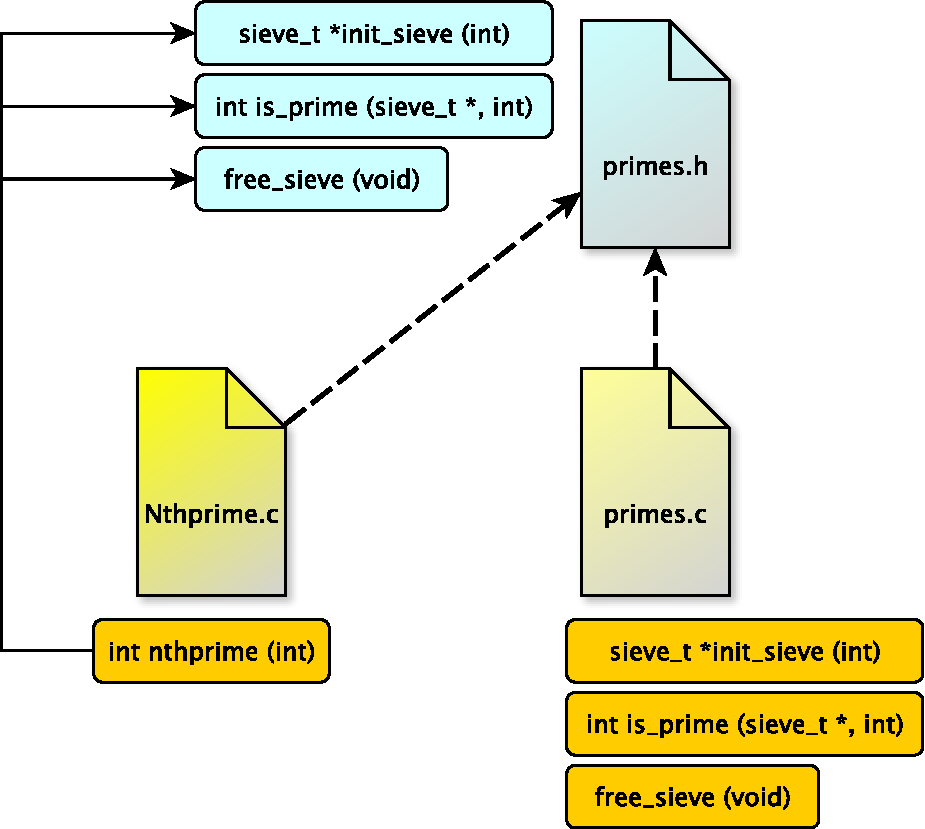
\includegraphics[width=0.8\textwidth]{illustrations/module-structure-crop.pdf}
\caption{Модульная структура программы}
\label{fig:module_struct}
\end{figure}

Если модуль primes.c достаточно стабилен, нет нужды каждый раз перекомпилировать его. Достаточно один раз скомпилировать его в специальный формат библиотечного файла -- libprimes.a или libprimes.so после чего подключать к линкеру опцией -lprimes. Но это уже платформенно-специфично, в windows речь идёт о DLL, в Linux может потребоваться PIC-код для so-модулей, etc. Всё это выходит за рамки курса, но достаточно легко осваивается по мануалам к вашей системе.

\textbf{Вопрос к студентам:} так ли нужны h-файлы? Что если непосредственно написать объявление \lstinline!init_sieve! в точке использования и предоставить линкеру самому найти тело этой функции.

\ifanswers
Правильный ответ: формально да, так можно сделать. Но реально единые заголовочники помогают бороться с человеческими ошибками. Когда изменяются типы параметров в точке определения, компилятор подскажет несоответствие заголовочнику и все места где их надо изменить в точке использования. Если же заголовочника не будет а программист забудет это сделать, будет тихое UB
\fi

\textbf{Домашняя наработка:} попробовать слинковать libprimes как статическую и как динамическую библиотеку и подключить к компиляции

\subsubsection{Призыв к саморазвитию}

Несмотря на то, что вся первая часть этих лекций посвящена повторению и углублению языка C, я во-первых призываю всех читать и перечитывать Кернигана и Ричи \cite{ritchie}, а во-вторых практиковаться в C, не забывая о нём при изучении C++. Лично я предпочитаю C и решения в стиле C за их простоту и близость аппаратуре.

Несколько дальнейших разделов посвящены более тонким вопросам, которые могли не рассматриваться в базовом курсе языка C, но могут быть нужны для понимания C++.

\pagebreak
\subsection{Дьяволы деталей синтаксиса C}\label{DevilDetails}

\hfill\textit{Probably the oddest aspect of C}

\hfill\textit{is the declaration syntax}{\vspace{0.5em}}

\hfill\textit{-- Dennis Ritchie}

В эпиграф вынесены (с некоторым сокращением) слова создателя языка C, сказанные им в интервью журналу C++ Report в 2000-м году, после нескольких десятков лет торжественного шествия языка по миру. И, в общем, человек знал что говорил. Пусть стоит задача прочитать простое объявление на языке C

\lstinputlisting[firstline=5,lastline=5]{cpp_code/p1s1.cpp}

\textbf{Вопрос к студентам:} что это? 

\ifanswers
Ответ: да, это массив указателей\index{Array of pointers}. 
\fi

\textbf{Вопрос к студентам:} как правильно написать указатель на массив?

\ifanswers
Ответ\index{Pointer to array}:

\lstinputlisting[firstline=6,lastline=6]{cpp_code/p1s1.cpp}
\fi

Теперь рассмотрим модификатор \lstinline!const!\index{const}. 

\textbf{Вопрос к студентам:} есть ли разница между следующими объявлениями:

\lstinputlisting[firstline=8,lastline=10]{cpp_code/p1s1.cpp}

\ifanswers
Ответ: между первым и вторым нет, между вторым и третьим очень существенная разница. Во втором случае (как и в первом) речь идёт о \textbf{не константном} указателе на константные данные. В третьем случае речь идёт о \textbf{константном} указателе на не константные данные. Объявляя константу нельзя оставить её неинициализированной, поэтому инициализатор выделяет строчку, где объявлен константный указатель. В то же время, указатель на константные данные сам может быть неконстантным и инициализации не требует (хотя она возможна).
\fi

\textbf{Вопрос к студентам:} как правильно написать константный указатель на константные данные? Сделать это надо двумя способами, не меньше.

\textbf{Вопрос к студентам:} что значит ключевое слово \lstinline!volatile!\index{volatile}, каковы способы его использования?

\textbf{Вопрос к студентам:} Запишите теперь константый указатель на волатильные данные. Имеет ли он смысл? Можете ли вы представить ситуацию, когда вам может понадобиться волатильный указатель на константные данные?

\ifanswers
Ответы на первые два вопроса очевидны, но ответ на третий может быть несколько экзотичен: если этот указатель \lstinline!register! переменная, которая определяет область памяти откуда идёт чтение и которая при этом соответсвует не настоящему регистру а некоему устройству, притворяющемуся регистром, но допускающему смену состояний, то конструкция обретает смысл.
\fi

Кроме того константность и волатильность также могут комбинироваться. Скажем возможен \lstinline!const volatile! указатель на \lstinline!const volatile! данные. В стандарте и прочих нормативных документах константность и волатильность любят объединять под общим названием ``cv-qualifier''\index{cv-qualifier} (C++14 3.9.3). Далее также будет употребляться термин ``cv-квалифи\-цированный тип'', это значит тип, к которому (возможно) добавлена константность, волатильность или обе сразу.

\textbf{Вопрос к студентам:} чем отличается \lstinline!const volatile int! от \lstinline!const int!?

\ifanswers
Правильный ответ: константность означает, что оттуда можно только читать. При этом волатильность означает, что чтения оттуда нельзя переупорядочивать. Интересно, что здесь \lstinline!const! это по сути способ сказать \lstinline!readonly!, чем семантически выразить неизменность данных.
\fi

\subsubsection{Чтение объявлений, как источник радости\index{C declarations}}\label{AlgDecl}

\textbf{Вопрос к студентам:} прочитайте объявление:

\lstinputlisting[firstline=12,lastline=12]{cpp_code/p1s1.cpp}

\ifanswers
Правильный ответ: указатель на функцию, возвращающую указатель на константный указатель на символ.
\fi

Алгоритм чтения таких объявлений (приведён например в \cite{linden}) следует из стандарта и в данном случае довольно прост:

\begin{itemize}
\item
Идём к имени переменной ``next''
\item
Группируем её с содержимым её скобок: ``next is a pointer to''
\item
За пределами скобок объявление функции имеет больший приоритет, поэтому ``next is a pointer to a function, returning''
\item
Далее обрабатываем слева звёздочку, имеем: ``next is a pointer to a function, returning pointer to''
\item
И далее парсим char * const: ``next is a pointer to a function, returning pointer to constant pointer to character''
\end{itemize}

В почти алгоритмическом виде, он изображен на рисунке (\ref{fig:cdecl_parse}). Также многие любят пользоваться специальными онлайн-приложениями, такими как \url{cdecl.org}.

\begin{figure}[h!]
\centering
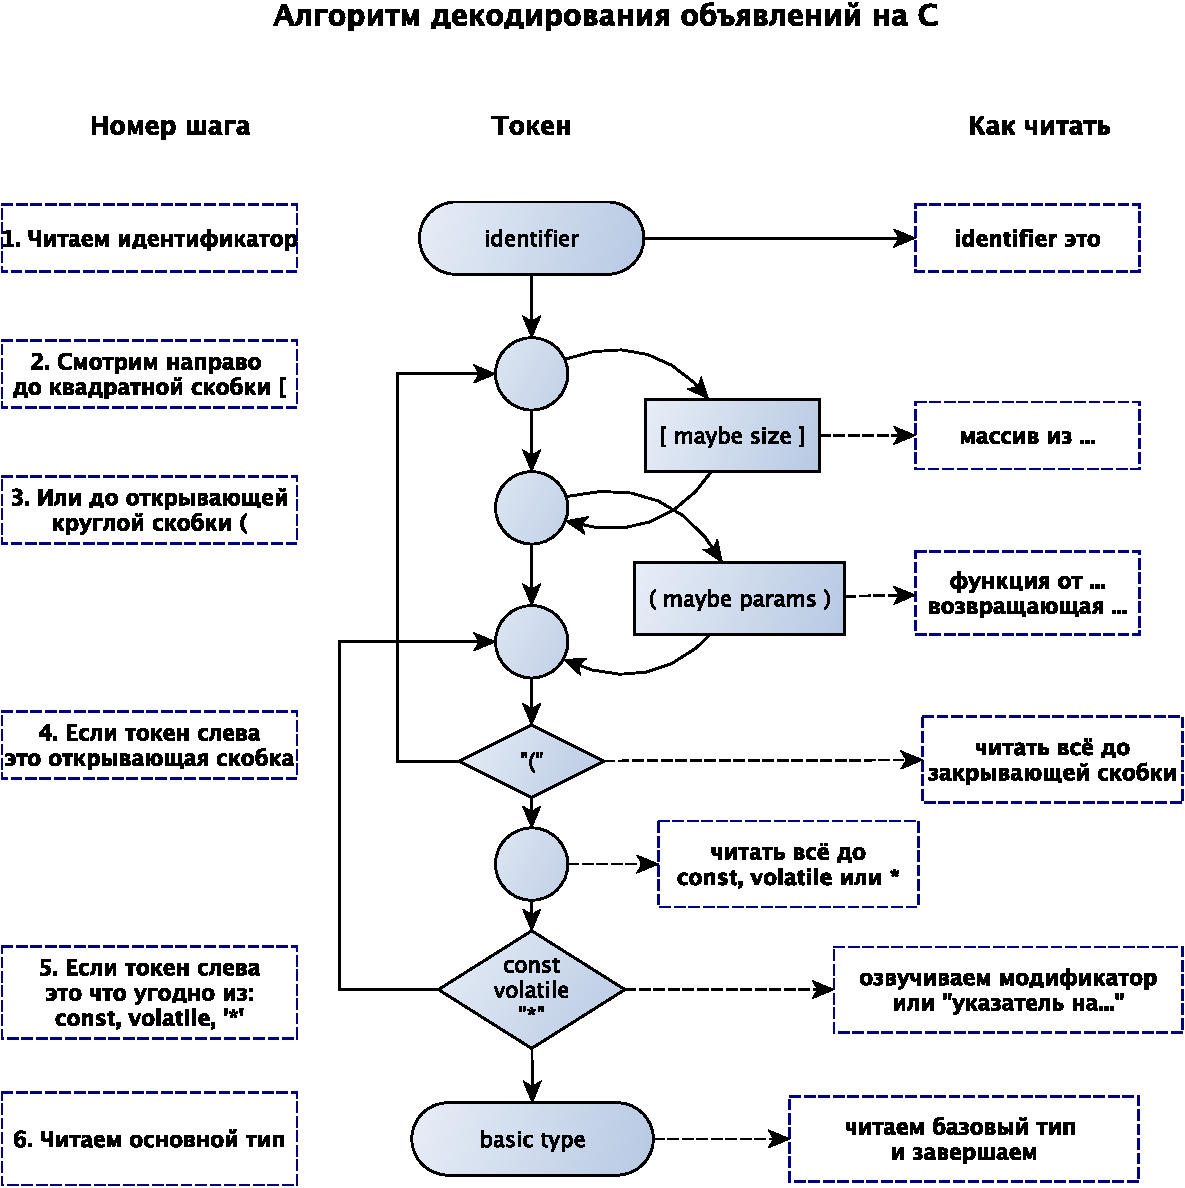
\includegraphics[width=1.0\textwidth]{illustrations/cdecls-crop.pdf}
\caption{Алгоритм разбора объявлений на C}
\label{fig:cdecl_parse}
\end{figure}

\textbf{Домашняя наработка:} по этому алгоритму написать программу, которая парсила бы произвольное объявление на C. Дополнительно: учесть возможность \lstinline!enum!, \lstinline!struct!, \lstinline!union!.

\textbf{Вопрос к студентам:} с учетом новых знаний, прочитать самостоятельно

\lstinputlisting[firstline=13,lastline=13]{cpp_code/p1s1.cpp}

\ifanswers
Ответ: c is array of 10 pointers to functions, accepting pointer to pointer to int and returning pointer to char.
\fi

\subsubsection{Ваш друг typedef\index{typedef}}\label{FriendTypedef}

Рассмотрим прекрасное объявление типа:

\lstinputlisting[firstline=15,lastline=15]{cpp_code/p1s1.cpp}

С помощью \lstinline!typedef! его можно переписать, доставив гораздо меньше боли глазам читающего (и без риска посадить случайную опечатку).

\lstinputlisting[firstline=16,lastline=17]{cpp_code/p1s1.cpp}

Ещё более хитрый способ упростить запись с использование расширений GCC рассмотрен в (\ref{SyntacticExts}), но он не особо переносим.

Умение читать запутанные объявление не означает необходимости их писать (если вы не участвуете в международном конкурсе по обфускации программ). Где возможно, следует использовать \lstinline!typedef!, это хороший стиль. Но хороший личный стиль (с другой стороны) это не основание не иметь навыка чтения запутанных объявлений. Каждый программист в жизни имеет дело с тоннами унаследованного кода, где встречается всякое.

У \lstinline!typedef! есть некоторые опасности, которые часто ускользают от новичков. Так например \lstinline!typedef! может объявить сразу несколько синонимов типов:

\lstinputlisting[firstline=19,lastline=19]{cpp_code/p1s1.cpp}

Это считается дурным тоном, старайтесь этого избегать. Ещё более дурным тоном считается зарыть typedef вглубь объявления, что тоже позволяется синтаксисом.

\lstinputlisting[firstline=20,lastline=20]{cpp_code/p1s1.cpp}

Опытный программист на языке C часто чувствует себя свободнее с препроцессором, скажем вместо

\lstinputlisting[firstline=21,lastline=21]{cpp_code/p1s1.cpp}

Есть соблазн написать

\lstinputlisting[firstline=22,lastline=22]{cpp_code/p1s1.cpp}

Но здесь есть тонкая ловушка:

\lstinputlisting[firstline=21,lastline=25]{cpp_code/p1s1.cpp}

Здесь переменные \lstinline!x! и \lstinline!y! будут разных типов, а \lstinline!w! и \lstinline!v! – одного типа.

\pagebreak
\subsection{Борьба с препроцессором}

\hfill\textit{Almost every macro demonstrates}

\hfill\textit{a flaw in the programming language,}

\hfill\textit{in the program, or in the programmer.}{\vspace{0.5em}}

\hfill\textit{-- Bjarne Stroustrup}

Пример с \lstinline!typedef! показывает, что использование возможностей языка лучше, чем использование препроцессора. Есть такие возможности C++, которые кардинально отличают программирование на C-подмножестве C++ и использование которых является хорошим тоном. Но есть и случаи, когда обойтись без препроцессора сложно.

\subsubsection{От макросов к константам времени компиляции}\label{ConstVsDef}

C-стилем в программировании является использование всюду препроцессора:

\begin{lstlisting}
#define BITS_PER_BYTE 8
#define sieve_type_bytes sizeof(sieve_type)
#define sieve_type_bits (sieve_type_bytes * BITS_PER_BYTE)
#define max_bit (1U << (sieve_type_bits - 1))
\end{lstlisting}

У такого подхода есть ряд недостатков: нет явного указания и контроля типов, происходит текстовая подстановка, в результате имена ``портятся'' для применения в программе, не пишется отладочной информации об именах констант и так далее.

В противоположность этому C++ подход состоит в явном задании хорошо типизированных констант:

\begin{lstlisting}
const unsigned BITS_PER_BYTE = 8;
const unsigned sieve_type_bytes = sizeof(sieve_type);
const unsigned sieve_type_bits = sieve_type_bytes * BITS_PER_BYTE;
sieve_type max_bit = (1U << (sieve_type_bits - 1));
\end{lstlisting}

Удивительно, что этот код не является корректным кодом на языке C, потому что в C одни константы не могут использоваться для инициализации других констант.

Ещё в большей степени это касается работы с перечислениями (строго говоря, она и в C была введена только в C99).

\begin{lstlisting}
/* C-style */
#define kword_TOKEN 10
#define kword_LITERAL 30
#define kword_SPACE 40
/* C++-style */
enum keyword {TOKEN = 10, LITERAL = 30, SPACE = 40};
\end{lstlisting}

Здесь кроме очевидной экономии места, вводится тип keyword, который может принимать только определённые в enum значения, что также является преимуществом.

\textbf{Вопрос к студентам:} видите ли вы какие-нибудь проблемы с таким подходом?

\ifanswers
Возможный ответ: да, символьное имя \lstinline!TOKEN! может конфликтовать с другим перечислением.
\fi

Кроме того, было бы очень хорошо иметь возможность в цикле пройти по всем элементам перечисления (сейчас это сложно, так как они не обязаны занимать не только последовательные, но даже и просто регулярно расположенные номера).

Более подробно эти проблемы и варианты их решения будут изложены несколько позже (см. \ref{EnumClass})

\subsubsection{Внешние, статические и встраиваемые функции}\label{Inline}

Любой идентификатор (переменная, функция) введенный в программе может иметь внешнее или внутреннее связывание (linkage specification). При разговоре о структуре программ (\ref{ProgramStructure}) уже было упомянуто, что линкер может найти функцию из одного модуля, объявленную в другом модуле. Но если бы это было верно для всех функций, две функции с одинаковыми именами не могли бы существовать в пределах всех единиц трансляции. 

К счастью, в C и в C++ функция может быть объявлена имеющей внутреннее связывание (модификатор \lstinline!static!), что означает, что она не экспортируется из модуля а используется только внутри него. Для указания внешнего связывания можно использовать ключевое слово \lstinline!extern! но вообще-то оно считается для функций указанным по умолчанию.

Обратите внимание: ключевое слово \lstinline!static! для переменной в глобальном диапазоне и внутри функции означает разные вещи. В глобальном диапазоне это ключевое слово означает внутреннее связывание, а внутри функции -- статическую переменную (то есть сохраняющую значение между вызовами функции).

Кроме внутреннего связывания, C и C++ поддерживают для функций (но не для переменных!) спецификатор \lstinline!inline!, обозначающий, что функция рекомендуется для встраивания: то есть вместо настоящего вызова, её тело будет размещено в точке вызова. Важно понимать, что использование ключевого слова \lstinline!inline! это не приказ, а совет, оно увеличивает шансы на подстановку но не обязует компилятор её производить.

\textbf{Вопрос к студентам:} если компилятор может не подставлять функцию, обозначенную как \lstinline!inline! и может подставить функцию не обозначенную таким образом, зачем вообще писать этот модификатор?

\ifanswers
Возможный ответ: \lstinline!inline! позволяет определение функции в каждом модуле (но увы это можно парировать тем, что для этого есть \lstinline!static!)
\fi

Правильный ответ: возможности компиляторов для встраивания как правило ограничены, так как слишком большой размер модулей это тоже плохо. Поэтому крайне часта ситуация, когда стоит выбор между несколькими функциями, каждую из которых можно встроить, но не все вместе. В этих случаях \lstinline!inline! помогает компилятору расставить приоритеты.

Благодаря встраиванию, C++ сильно выигрывает для определения небольших функций, где в C были выгодны макросы. Хороший пример -- вычисление максимума двух чисел.

Типичный контекст использования

\begin{lstlisting}
int a = 5, b = 0;
assert (MAX(a,b) == 5);
\end{lstlisting}

Вариант реализации на C:

\begin{lstlisting}
#define MAX(a, b) ((a) > (b) ? (a) : (b))
\end{lstlisting}

Вариант реализации на C++:

\begin{lstlisting}
static inline long
MAX (long a, long b)
{
  return (a > b) ? a : b;
} 
\end{lstlisting}

Оба эти варианта работают. Но теперь можно представить более сложный случай:

\begin{lstlisting}
int a = 5, b = 0;
int c = MAX(++a, b);
int d = MAX(++a, b+10);
\end{lstlisting}

\textbf{Вопрос к студентам:} что будет содержаться в \lstinline!c! и в \lstinline!d!? А что если подставить вызов функции \lstinline!max!? 

\ifanswers
Правильный ответ: макрос раскроется как \lstinline!((++a) > (b) ? (++a) : (b))! то есть в сишной версии \lstinline!a! будет инкрементирована дважды. В C++ версии всё норм.
\fi

Пока что сишный вариант, тем не менее, обладает некоторой притягательностью: если исключить сайд-эффекты, то во-первых он является безразличным относительно типов аргументов (type generic), так что его можно использовать и для \lstinline!double! в то время, как плюсовый вариант как он сейчас написан, требует только чисел типа \lstinline!long!. В (\ref{FunctionTemplate}) будут рассмотрены средства, которые позволяют написать обобщенный максимум на C++

Есть ещё аргумент относительно штрафа на производительность из-за вызова функции. Но поскольку вызов \lstinline!max! почти всегда будет проинлайнен, эффективность C++ метода как минимум не страдает. Более того, почти всегда, когда в C использовался \lstinline!void*! для передачи параметров неопределённого типа, в C++ можно написать более эффективный код, используя шаблоны. Подробный разбор этого следует несколько отложить (см. \ref{FunctionTemplate}).

Удивительно, но даже без встраивания функций, замена макросов на функции может дать прирост производительности

\begin{lstlisting}
#define SQR(x) ((x)*(x))
unsigned sqr (x) { return x*x; }
\end{lstlisting}

в контексте использования

\begin{lstlisting}
unsigned t = SQR(f(x));
\end{lstlisting}

Если возведению в квадрат подвергается результат вычисления функции \lstinline!f!, то вариант с макросом вызовет её дважды, а вариант с функцией вызовет её один раз.

Модификатор \lstinline!inline! появился и в языке C (начиная с C99) но там он работает по другим правилам: функция, объявленная \lstinline!inline! по умолчанию считается не \lstinline!static! а \lstinline!extern!. Внешние встраиваемые функции означают, что в каждом модуле вы должны предоставить тело такой функции для возможного встраивания, но, если встраивания не произойдёт, будет вызвана та из них, где \lstinline!extern! указан явно.

На C++ \lstinline!extern inline! тоже можно писать, но тут правила гораздо мягче: стандарт всего лишь требует от линкера выбрать какую-то одну реализацию чтобы сгенерировать из неё тело для вызова (C++14 7.2.1).

\textbf{Вопрос к студентам:} в чём по-вашему может быть смысл писать \lstinline!extern inline! функции?

\ifanswers
Возможный ответ: семантика статических переменных -- внутри \lstinline!static inline! функций создается столько их копий сколько функций, внутри \lstinline!extern inline! копия одна на всех.
\fi

\subsubsection{Когда нужен препроцессор}

В некоторых случаях препроцессор всё-таки нужен. Так, например, в (\ref{ProgramStructure}) был описан случай включения заголовочных файлов с использованием \lstinline!#include!. Возможно в стандарте C++17 пройдет предложение по модулям в языке и тогда эта практика станет устаревшей, но пока это единственная (и хорошо проверенная временем) возможность организовать модульность.

Также почти всегда нужны стражи включения, позволяющие не включать один и тот же модуль дважды. Например в ситуации когда в процессе включения возникает циркулярная ссылка, они бывают полезны чтобы прервать её. Но и вообще простановка стражей включения это хороший тон, так что реальный модуль primes.h из (\ref{ProgramStructure}) будет выглядеть как-то так:

\begin{lstlisting}
#ifndef PRIMES_GUARD_
#define PRIMES_GUARD_

/* ... something meaningfull ... */

#endif
\end{lstlisting}

Ещё один случай это отключение неиспользуемого кода по опции сборки

\begin{lstlisting}
#ifndef VERBOSE
#define VERBOSE 0
#endif

#if (VERBOSE == 1)
/* ... some logging ... */
#endif
\end{lstlisting}

Эта программа скомпилированная с \lstinline!-DVERBOSE=1! будет выполнять дополнительный код, заключенный под директиву препроцессора.

Иногда нужно использовать черную магию препроцессора, например возможности по конкатенации:

\begin{lstlisting}
struct command
{
  char *name;
  void (*function) (void);
};
     
struct command commands[] =
{
  { "quit", quit_command },
  { "help", help_command },
  /* ..... */
};
\end{lstlisting}

Гораздо яснее и проще

\begin{lstlisting}
#define COMMAND(NAME)  { #NAME, NAME ## _command }
     
struct command commands[] =
{
  COMMAND (quit),
  COMMAND (help),
  /* ..... */
};
\end{lstlisting}

Это уберегает от человеческих ошибок (скажем несоответствия имени хендлеру), но использование таких конструкций должно быть исключением, а не правилом.

Иногда применение препроцессора связано с необходимостью трюков для применения по косвенности:

\textbf{Вопрос к студентам:} что ниже следует поставить, чтобы добиться искажения функции по значению переменной:

\begin{lstlisting}
#define VARIABLE 3

/* ... some magic? ... */

extern void NAME(mine)(char *x);
/* creates mine_3 function */
\end{lstlisting}

\ifanswers
Правильный ответ должен включать не менее трёх уровней косвенности:

\begin{lstlisting}
#define PASTER(x,y) x ## _ ## y
#define EVALUATOR(x,y)  PASTER(x,y)
#define NAME(fun) EVALUATOR(fun, VARIABLE)
\end{lstlisting}

Порядок расширения макросов следующий:

\begin{lstlisting}
NAME(mine)
EVALUATOR(mine, VARIABLE)
PASTER(mine, 3)
\end{lstlisting}

Поэтому пропустить хотя бы один уровень косвенности здесь нельзя.
\fi

Все эти случаи, как можно заметить, касаются базового применения препроцессора: для обработки текста программы. Во всех остальных случаях при программировани на C++ использования препроцессора стараются избегать.

\pagebreak
\subsection{Базовые концепции языка}\label{BasicTerms}

Есть существенное отличие между знанием как работает язык и знанием почему он так работает. Стандарты языков и руководства по программированию часто написаны в очень разных терминах. В основе C++ лежит целая совокупность фундаментальных понятий: точки объявления и инстанцирования, полные и неполные типы, правые и левые ссылки, области видимости и спецификаторы связывания. Все они крайне важны. В этом разделе будет рассмотрено некоторое количество таких корневых концепций, без которых дальнейшее понимание языка будет затруднено.

\subsubsection{Объявления и определения\index{declaration}\index{definition}}\label{DeclVsDef}

До сих пор действия с объявлениями и определениями выполнялись интуитивно, без полного понимания того, что это такое. Настало время обратить внимание на детали.

Объявление (declaration) это введение идентификатора и описание типа.

\begin{lstlisting}
extern int bar;
extern int g(int, int);
double f(int, double); /* extern can be omitted for function declarations */
class foo; /* no extern allowed for class declarations */
\end{lstlisting}

Нужно обратить внимание на перегруженность ключевого слова \lstinline!extern!: в (\ref{Inline}) оно использовалось для задания внешнего/внутреннего связывания, тогда как здесь используется оно же, но для указания, что переменная объявлена, но не определена.

Объявление достаточно компилятору, чтобы разрешить ссылки на данный идентификатор. 

Определение это реализация типа или выделение памяти объекту.

\begin{lstlisting}
int bar;
int g(int lhs, int rhs) {return lhs*rhs;}
double f(int i, double d) {return i+d;}
class foo {};
\end{lstlisting}

Определение достаточно линкеру, чтобы реализовать идентификатор в объектном коде. 

Объявление может встречаться сколько угодно раз. Определение встречается лишь один раз. Это называется One Definition Rule (ODR\index{ODR}) и оно должно чётко соблюдаться. Нарушение ODR -- UB. При этом любое определение также является объявлением.

У ODR есть несколько уровней строгости и из него есть несколько исключений, см. (C++14 3.2) где они перечислены.

\begin{itemize}
\item функции и переменные с внешним связыванием должны быть определены один раз на все единицы трансляции
\item встраиваемые (inline) функции, статические (static) функции и переменные, определения пользовательских типов, шаблоны классов и их частичные специализации должны быть определены не более одного раза в каждой единице трансляции
\end{itemize}

Можно запомнить мнемоническое правило чтобы не путать объявление с определением, а в англоязычной литературе declaration и definition, нужно смотреть на словарное упорядочение.  Буква ``б'' расположена раньше, чем ``п''. Значит в словаре слово ``объявление'' будет раньше, чем ``определение'' и так же declaration в английском словаре идёт раньше, чем definition. И так же в программе – объявление всегда должно идти раньше определения.

Не стоит путать также определение переменной и её инициализацию. Переменная может быть определена но не инициализирвоана. В C и в C++ чтение неинициализированной переменной это UB (например C99 6.3.2.1/2).

Важной концепцией является точка объявления (PoD, Point of Declaration) \index{Point of Declaration}. Объявление имени считается законченным когда записан полный идентификатор (то есть \textbf{до} возможных инициализаторов). Поэтому:

\begin{lstlisting}
int x = 2;
{
  int x /* PoD */ = x;
}
\end{lstlisting}

В этом случае значение внутреннего \lstinline!x! не определено. Но в следующем случае:

\begin{lstlisting}
int x = 2;
{
  int x[x] /* PoD */;
}
\end{lstlisting}

всё корректно и вложенный массив имеет два элемента.

\textbf{Вопрос к студентам:} хорошо, в первом случае оно не определено. Но если программа будет, тем не менее, читать значения из такой неинициализированной переменной, будет ли каждый раз получаться одно и то же (пусть мусорное) значение или могут быть всегда разные?

\ifanswers
Ответ: могут быть всегда разные, так как UB
\fi

Интересно, что строчка одного и того же вида может служит определением или объявлением в зависимости от контекста:

\begin{lstlisting}
typedef void T();
T t; /* declaration of function "t" */

struct X 
{ 
  T t; /* declaration of function "t" */
};

typedef int T;
T t; /* definition of object "t" */
\end{lstlisting}

Эта ассимметрия связана с (исторической) ассиметрией объявлений функций и переменных.

Также при определении не должен сужаться объявленный linkage specifier, поэтому вот так можно:

\begin{lstlisting}
static int x;
extern int x;
\end{lstlisting}

А вот так нельзя:

\begin{lstlisting}
extern int x;
static int x;  /* BOOM! */
\end{lstlisting}

Во втором случае storage class переменной уже заявлен как внешний и не может быть переопределен.

Больше про объявления и определения классов в (\ref{DeclDefs}).

\subsubsection{Область видимости и время жизни}\label{ScopeLifeTime}

С концепцией точки объявления, связана концепция области видимости. Область видимости \index{Scope} переменной, объявленной внутри блока из фигурных скобок это текст программы от точки определения до закрывающей фигурной скобки блока. В стандарте можно посмотреть правила для других областей видимости (C++14 3.3).

Гораздо более интересной концепцией является время жизни переменной. Время жизни переменной бывает не равно её области видимости.

Область видимости (scope) это те места в программе, где возможно обращение к переменной.

Время жизни (lifetime) это все то время, когда значение переменной валидно.

Для автоматических и нелокальных статических переменных, их время жизни почти всегда совпадает с областью видимости.

\textbf{Вопрос к студентам:} охарактеризуйте следующий код:

\begin{lstlisting}
int foo(int x) 
{
  int y, *p;

  {
    int z = 5; 
    p = &z;
  }

  y = *p;
  return y;
}
\end{lstlisting}

\ifanswers
Правильный ответ: этот код демонстрирует undefined behavior. В точке разыменования указателя истекло время жизни того, на что он указывает.
\fi

\textbf{Вопрос к студентам:} теперь охарактеризуйте следующий код:

\begin{lstlisting}
int foo(int x) 
{
  int y, *p;

  {
    static int z = 5; 
    p = &z;
  }

  y = *p;
  return y;
}
\end{lstlisting}

\ifanswers
Правильный ответ: здесь работает ещё одна перегруженная функция ключевого слова \lstinline!static! -- оно расширяет время жизни переменной до времени жизни программы. Таким образом здесь будет все хорошо -- переменная \lstinline!z! будет жить даже между вызовами функции.
\fi

Вещи становятся сложнее, когда в игру вступает динамическая память:

\begin{lstlisting}
int* 
f (int n) 
{
  int *p = malloc (sizeof(int) * n); /* 1 */
  return p;
} /* 2 */

int 
main () 
{
  int *q = f (10); 
  free (q); /* 3 */
}
\end{lstlisting}

Здесь область видимости переменной \lstinline!p! заканчивается в точке 2, а время жизни объекта в динамической памяти -- в точке 3.

С указателями все ещё интереснее: оказывается само время жизни указателя зависит от жизни объекта, на который он указывает. Стандарт регламентирует (C99 6.4.2), что ``The value of a pointer becomes indeterminate when the object it points to reaches the end of its lifetime''. Например:

\begin{lstlisting}
int *p = malloc (sizeof(int));
long pold = (long) p;
free (p);
assert (p == (int *)pold); /* ORLY? */
\end{lstlisting}

Здесь время жизни \lstinline!p! закончилось, хотя \lstinline!p! это локальная переменная и она не выходила из области видимости.

На самом деле, время жизни оканчивает не только \lstinline!free! но и \lstinline!realloc!. Известный технический анекдот основан на так называемом ``N. Lewycky realloc'' (реаллок Левицкого). Ник Левицкий, инженер LLVM compiler team предложил следующий код

\begin{lstlisting}
int *p = malloc (sizeof(int));
int *q = realloc (p, sizeof(int));
*p = 1;
*q = 2;
if (p == q) {
  printf ("%d %d\n", *p, *q);
}
\end{lstlisting}

И на тогдашнем clang, этот код распечатал ему ``1 2'', что, вообще говоря, безумие, потому что получается, что в программе есть два одинаковых указателя, которые указывают на разные объекты.

Конечно здесь UB из-за использования указателя после \lstinline!realloc! т.е. после окончания времени жизни.

\subsubsection{Полные и неполные типы}

Если тип (структура, класс, массив) только объявлен, но не определен то этот тип считается неполным. Полным тип становится только в точке, в которой встречается его определение. Но даже неполного типа вполне хватает для объявлений. На примере структур:

\begin{lstlisting}
struct t; /* declare type t */

extern int foo(t p); /* ok, incomplete function type */
extern t x; /* ok, incomplete variable */
extern t arr[]; /* ok, incomplete array */
\end{lstlisting}

\textbf{Вопрос к студентам:} можно ли написать определение объекта неполного типа?

\ifanswers
Правильный ответ: конечно нет, так как неизвестно сколько памяти надо такому объекту. Но можно написать определение указателя на такой объект.
\fi

\subsubsection{Lvalue и rvalue\index{lvalue}\index{rvalue}}\label{LRvalues}

Следующий пример, многим может показаться излишне простым.

\begin{lstlisting}
x = y;
\end{lstlisting}

Что здесь написано? Здесь написано – взять адрес переменной \lstinline!x! и записать по этому адресу значение переменной y. В этом выражении присваивания, переменная \lstinline!x! находится в выражении слева, а \lstinline!y! -- справа и стандарт C++98 вводит специальные термины rvalue (right-hand-side value) и lvalue (left-hand-side value) интуитивно понимаемые как ``нечто, что может быть справа (слева) в выражении присваивания'' (C++98 3.10). 

Итак, какие ограничения этот пример накладывает на \lstinline!x!? Похоже, что \lstinline!x! должен быть полного типа, не константым, и иметь определённое местоположение в памяти (быть адресуемым). Есть ли ограничения на \lstinline!y!? Да есть. Он должен быть полного типа и этот тип должен быть совместим с типом \lstinline!x! по присваиванию.  

Это типичный пример того, как компилятор может решить из контекста (в данном случае из положения справа или слева от присваивания) будет ли он использовать адрес переменной или её значение в своих фактических вычислениях. Такая возможность у компилятора есть, потому что адрес переменной полного типа всегда известен во время компиляции и нет необходимости заставлять программиста его специально получать.

\begin{lstlisting}
*(&x) = y;
\end{lstlisting}

Возможно, кстати, писать так было бы честнее.

Стандарт C++11 существенно расширяет и дополняет классификацию категорий значений, речь об этом пойдет в (\ref{LRvaluesAgain}).

\pagebreak
\subsection{Массивы и указатели}\label{ArrPointers}

\hfill\textit{Should array indices start at 0 or 1?}

\hfill\textit{My compromise of 0.5 was rejected without,} 

\hfill\textit{I thought, proper consideration}{\vspace{0.5em}}

\hfill\textit{-- Stan Kelly-Bootle}

Многие программисты заучивают правило для новичка: массивы в C это указатели и наоборот. Это правило, пожалуй, действительно полезно для новичка. Но в общем случае это не так. В этом разделе будут проведены чёткие разграничения. 

\subsubsection{Вспоминаем указатели}

Указатель хранит адрес, по которому программа может прочитать и (в случае неконстантных данных) записать значение, того типа, из которого выведен тип указателя. Для любой переменной на протяжении её времени жизни (\ref{ScopeLifeTime}) стандарт гарантирует побитовую неизменность адреса (C11 6.2.4).

С неконстантным указателем можно сделать следующее:

\begin{enumerate}
\item Объявить и инициализировать константой
\begin{lstlisting}
int *x = 0;
\end{lstlisting}
\item Объявить и инициализировать адресом переменной или функции
\begin{lstlisting}
struct str_t {int x; int y;};
int foo (int x);
int c = 2;
str_t s = {1, 2};
int *p = &c;
int (*pfoo) (int) = &foo;
str_t *ps = &s;
\end{lstlisting}
\item Присвоить иное значение
\begin{lstlisting}
int bar (int x);
p = x;
x = &c;
pfoo = &bar
\end{lstlisting}
\item Разыменовать и получить или изменить значение
\begin{lstlisting}
c = *x;
*p = 5;
c = (*ps).x;
c = ps->x;
ps->x = *p;
\end{lstlisting}
\item Использовать индексацию, похожую на массив
\begin{lstlisting}
p[0] = c;
*(p+0) = c;
\end{lstlisting}
\item Возвращать из функций
\begin{lstlisting}
int *foo (int x) { return &x; }
\end{lstlisting}
\end{enumerate}

Неконстантные указатели являются lvalue. В принципе, можно записать:

\lstinputlisting[firstline=26,lastline=28]{cpp_code/p1s2.cpp}

Этот код является дурным тоном, он будет плохо переносим и совершенно точно тут указатель используется не по назначению, но важно, что это можно сделать. Указатель это честная ячейка памяти. Он хранит то, что туда положил программист, как это показано на рисунке \ref{fig:pointers}.

\begin{figure}[h!]
\centering
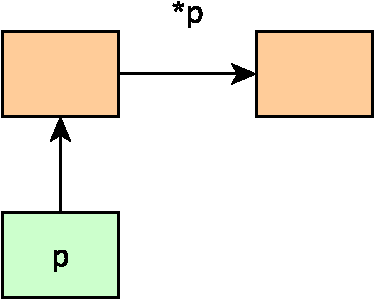
\includegraphics[width=0.3\textwidth]{illustrations/pointers-crop.pdf}
\caption{Визуальное представление указателей}
\label{fig:pointers}
\end{figure}

\textbf{Вопрос к студентам:} можно ли сериализовать указатели, например в файл, а потом восстанавливать и использовать?

\ifanswers
Ответ: да, в течении срока жизни того, на что они указывают.
\fi

\textbf{Вопрос к студентам:} можно ли для переменной сказать сколько указателей на неё в данный момент существует?

\ifanswers
Ответ: увы, нет. Никакая переменная не ``знает'' о том, что кто-то взял её адрес и т.п.
\fi

Это, вообще говоря, сильно снижает возможности компиляторов к оптимизации:

\begin{lstlisting}
float *b; 
int x;
/* ... */
x = 1;
*b = 5;
x = x + 3;
foo (x);
}
\end{lstlisting}

Эта функция могла бы быть оптимизирована к:

\begin{lstlisting}
x = 4;
*b = 5.0;
foo (4);
\end{lstlisting}

Но компилятор не имеет права этого делать: в строчках кода помеченных троеточием вполне могло встретится нечто вроде:

\begin{lstlisting}
b = (float *) &x;
\end{lstlisting}

И в этом случае запись \lstinline!*b = 5.0! непредсказуемо изменит \lstinline!x!.

В связи с этим, сообществом и большинство компиляторов (но не стандартом) поддерживаются \textbf{strict aliasing rules}\index{strict aliasing}\label{StrictAliasing}. Их суть -- в запрещении доступа к данным одного типа по указателю другого типа. Большинство компиляторов проверяют strict aliasing по умолчанию и требуют специальных опция для его отключения.

Кроме того, в стандарте языка C99 (но не C++) для указателей поддерживается модификатор \lstinline!restrict! (C99 6.7.3)

\begin{lstlisting}
void 
f (int n, int * restrict p, int * restrict q)
{
  while (n-- > 0)
  *p++ = *q++;
}
\end{lstlisting}

Здесь программист как бы дает компилятору обещание, что на вход \lstinline!f! придут непересекающиеся области данных.

\subsubsection{Арифметика указателей}

Кроме всего прочего, указатели можно складывать с целыми числами, а также вычитать из них целые числа и указатели друг из друга.

Для сложения, указателем может быть любой из операндов (но только один из них, сложить два указателя нельзя). Для вычитания обязательно левый операнд должен быть указателем, а правый -- указателем или числом

\begin{lstlisting}
int arr[] = {0, 1, 2, 3, 4, 5};
int a = 0; 
int *b = &arr[0];
int *c = b + a; /* ok */
int *d = a + b; /* ok */
int *e = c + d; /* error */
ptrdiff_t f = c - d; /* ok */
int *g = c - a; /* ok */
int *h = a - c; /* error */
\end{lstlisting}

Следует обратить внимание на тип \lstinline!ptrdiff_t! в коде выше -- это специальный тип, достаточно широкий, чтобы хранить разность указателей. Следует по возможности пользоваться им, но, как запасной вариант, есть тип \lstinline!long! (которого увы не хватает для LLP64 систем, таких как Win64, но он вполне пригоден для почти всех unix-специфичных приложений). Он находится в хедере \lstinline!<stddef.h>!.

\textbf{Вопрос к студентам:} как вы думаете возможно ли посчитать разницу между указателями на стеке и в куче?

\begin{lstlisting}
int *t = malloc (sizeof(int));
int k = 4;
ptrdiff_t d = t - &k; /* ok? */
\end{lstlisting}

\ifanswers
Правильный ответ: разумеется да, адресная арифметика по стандарту прозрачна относительно того где расположена память до тех пор, пока все влезает в \lstinline!ptrdiff_t!.
\fi

\subsubsection{Нулевые указатели}\label{NullPointers}

Особой разновидностью указателей являются нулевые указатели. Первое, что нужно о них запомнить: нулевой указатель может быть не нулевым. В этом смысле константы \lstinline!0!, \lstinline!NULL! или, скажем, \lstinline!nullptr! из нового стандарта это разные константы. Для конкретной архитектуры значение \lstinline!NULL! может быть \lstinline!0xffff0000!, или любым другим.

Но во всех распространенных архитектурах \lstinline!NULL == 0! и чтобы сохранить обратную совместимость существующего кода, стандарт определяет правила неявной конверсии \lstinline!0! в \lstinline!NULL! при сравнении с ним указателей (C99 6.3.2.3).

\begin{lstlisting}
int *t = malloc (sizeof(int));
assert (t); /* ok */
\end{lstlisting}

Здесь условие под \lstinline!assert! будет неявно сконвертировано в правильную форму. Конечно, программист, заботящийся о стиле, сразу пишет правильно:

\begin{lstlisting}
int *t = malloc (sizeof(int));
assert (t != NULL); /* great */
\end{lstlisting}

Но и в первом варианте нет ошибки.

\textbf{Вопрос к студентам:} но ведь ноль может быть не только вбит, но и предвычислен:

\begin{lstlisting}
int *zerop = (int*)(x – y);
assert (zerop == NULL);
\end{lstlisting}

Представим, что в этом случае \lstinline!NULL == 0xffff0000! и при этом \lstinline!x == y!. Сработает ли assertion?

\ifanswers
Правильный ответ: увы, нет. Стандарт гарантирует стабильное обращение с нулями времени компиляции, но не нулями времени исполнения (C99 6.3.2.3), иначе проверками пришлось бы завешивать слишком много кода.
\fi

\subsubsection{Действия с массивами}

Встроенные массивы (также C-массивы) исторически предшествовали указателям и представляют собой простейший вид синтаксического клея -- логически непрерывную область памяти, побитую на однотипные ячейки.

С массивами также возможны некоторые действия.

\begin{enumerate}
\item Объявить и инициализировать списком данных (все пропущенные инициализаторы -- нулевые)
\begin{lstlisting}
int a = 5;
int x[10] = {6, a};
\end{lstlisting}

Следует обратить внимание: неинициализированным может быть только локальный массив. Глобальные массивы всегда инициализированы нулями.

Также следует обратить внимание. Определение вида:
\begin{lstlisting}
int wrong[]; /* boom! */
\end{lstlisting}
Это ошибка (поскольку компилятор не знает сколько памяти выделять на этот массив). Но можно использовать такой синтаксис в объявлениях
\begin{lstlisting}
extern int wrong[]; /* ok */
\end{lstlisting}
\item Прочитать или записать значение
\begin{lstlisting}
int t = x[0];
x[1] = t;
x[0] = x[1];
\end{lstlisting}
\item Деградировать (decay) к указателю если он используется как rvalue\label{ArrDecaying}\index{Decay}
\begin{lstlisting}
int foo (int *t);
int *p = &x[0];
*p = x; /* decay */
a = *(x + 3); /* decay */
a = foo (x + 5); /* decay */
\end{lstlisting}
\end{enumerate}

\begin{figure}[h!]
\centering
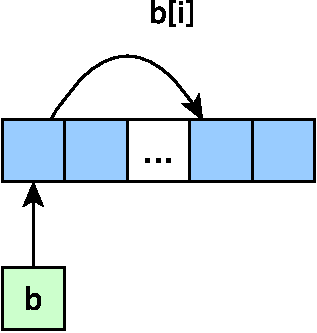
\includegraphics[width=0.3\textwidth]{illustrations/arrays-crop.pdf}
\caption{Визуальное представление массивов}
\label{fig:arrays-crop}
\end{figure}

Но массивы \textbf{никогда} не употребляются вместо указателей там, где указатель это lvalue.

\begin{lstlisting}
int v = 5;
int *p = &v;
int a[1] = {v};
p = a; /* ok */
a = p; /* never */
\end{lstlisting}

По той же причине нет возможности вернуть массив из функции:

\begin{lstlisting}
typedef int arr_t[10];

arr_t foo (void); /* Error! */
\end{lstlisting}

Разумеется, невозможна никакая арифметика массивов -- прибавить один массив к другому или вычесть один массив из другого в языке C невозможно.

Массивы хранят сами данные, а не указатели на них. То, что они синтаксически могут вырождаться к указателям -- удобная концепция, связанная с ранней историей массивов в языке C и в дальнейшем получившая неожиданно глубокое и мощное развитие в последних версиях стандарта C++ (см. \ref{Decaying}). Массив содержит lvalue-ячейки данных, но сам как целое он не является lvalue-ячейкой данных.

\subsubsection{Инициализация массивов и указателей}

Инициализация массивов и указателей выглядит похоже, но означает разные вещи:

\lstinputlisting[firstline=35,lastline=37]{cpp_code/p1s2.cpp}

\textbf{Вопрос к студентам:} есть ли разница между этими двумя записями и какую вы предпочтёте? Почему?

\ifanswers
Верный ответ: строчка 1 предпочтительней, чем (устаревшая, с Wall + Werror выдаст ``error: deprecated conversion from string constant to \lstinline!char*!'') строчка 2 и они имеют разную семантику. Память под массивы выделяется автоматически (и строчка 1 подразумевает неявный memset) но память никогда автоматически не выделяется под указатели, поэтому для построения динамических структур данных (например, связных списков) используются указатели, а не массивы.
\fi

Между прочим, строковые литералы в инициализации указателей это счастливое (исторически сложившееся) исключение. Строчка 2 в следующем примере не будет скомпилирована:

\lstinputlisting[firstline=43,lastline=44]{cpp_code/p1s2.cpp}

\textbf{Вопрос к студентам:} есть ли разница между следующими двумя объявлениями?

\begin{lstlisting}
int foo (int x[]);
int foo (int *x);
\end{lstlisting}

\ifanswers
Ответ: из-за decaying разницы нет.
\fi

\textbf{Вопрос к студентам:} означает ли эта запись:

\begin{lstlisting}
int foo (int x[16]);
\end{lstlisting}

что \lstinline!foo! принимает массив из 16 символов?

\ifanswers
Ответ: нет, здесь \lstinline!foo! принимает любой указатель.
\fi

\subsubsection{Прогулки за границами}

Хорошо написанный код никогда не должен ничего считывать и записывать за границами массивов. В общем случае проблема доступа к данным вне выделенного для доступа буфера называется ``buffer overflow'' или ``buffer underflow'' и является (не только в C) одним из основных источников уязвимостей программ. Увы, такие языки как C имеют к нему родовую предрасположенность: максимальная эффективность требует отсутствия неявных проверок времени выполнения.

К чему это приводит можно проиллюстрировать на примере простейшей уязвимости:

\begin{lstlisting}
char buff[16];
int pass = 0;

printf("\n Enter the password : \n");
gets(buff);

if (strcmp (buff, "correctpassword"))
  {
    printf ("\n Wrong Password \n");
  }
else
  {
    printf ("\n Correct Password \n");
    pass = 1;
  }

if (pass)
  {
    /* Now Give root or admin rights to user*/
    printf ("\n Root privileges given to the user \n");
  }
\end{lstlisting}

Здесь чтобы демонстрация была эффектной придется скомпилировать без оптимизаций чтобы переменная попала на стек:

\begin{verbatim}
$ g++ p1-overrun.cpp -O0 -m32
$ ./a.out
Enter the password : 
hhhhhhhhhhhhhhhhh

 Wrong Password 

 Root privileges given to the user 
\end{verbatim}

Введен очевидно неверный пароль. Но поскольку он переполняет стек, последний символ записывается в переменную \lstinline!pass! и таким образом её значение меняется и пароль засчитывается как верный.

Это самый простой, можно сказать ``детский'' пример такой уязвимости, в реальности всё сложнее и разнообразнее, но идея именно эта.

Частично защититься от порчи стека в GCC может помочь опция \lstinline!-fstack-protector-all! -- с ней программа просто упадет, оставив трассу

\begin{verbatim}
$ g++ p1-overrun.cpp -O0 -m32 -fstack-protector-all
$ ./a.out 

 Enter the password : 
hhhhhhhhhhhhhhhhh

 Wrong Password 
*** stack smashing detected ***: ./a.out terminated
\end{verbatim}

Если вы используете другой компилятор, у него скорее всего существуют аналогичные средства, кроме того существует целый класс бесплатных и коммерческих программ (их хорошо искать по ключевым словам bounds checking).

Эти программы, конечно, тоже не панацея. Большинство из них (включая защиту стека в GCC) отлавливают только уже произошедшую запись в неправильное место на стеке, реально же проблемы с уходом за границу массива могут быть гораздо более тонкими и даже вообще не включать порчи стека. Например по стандарту арифметика указателей в пределах массива не должна уходить дальше, чем на один элемент от границ массива:

\begin{lstlisting}
int arr[] = {0, 1, 2, 3, 4, 5};
int *a = arr; /* ok, decaying as &arr[0] */
int *b = a + 3; /* ok, *b == 3 */
int *c = a + 6; /* ok, c is one past arr */
int *d = a + 7; /* undefined behavior */
d = d - 4; /* even here, *d is undefined */
\end{lstlisting}

Пятая строчка здесь создает UB и весь код поcле этой строчки теряет предсказуемость. Даже если программа, ничего не меняя за границами массива, ``честно'' возвращается в допустимую область, тем не менее, UB уже случилось, жесткий диск уже отформатирован, всё пропало.

\subsubsection{Многомерные массивы\index{multidimensional arrays}}\label{MultiDimArr}

Настоящий многомерный массив (вообще -- настоящий массив) это абстрактный тип данных \lstinline!A!, для которого определены две операции \lstinline!get(A, I)! и \lstinline!set(A, I, V)!. При этом выполняются аксиомы:

$get(set(A,I,V),I)=V$

$get(set(A,I,V),J)=get(A,J)|I \neq J$

В качестве индекса служит кортеж произвольных объектов, обычно целых чисел.

Язык C и C-подмножество языка C++ не поддерживают семантику многомерного массива на уровне языка.

Хуже того, существует противоречие между статическими многомерными массивами (которые на самом деле одномерные с хитрым доступом) как на (рис. \ref{fig:c_arrays}) и динамическими многомерными массивами (там же).

\begin{figure}[h!]
\centering
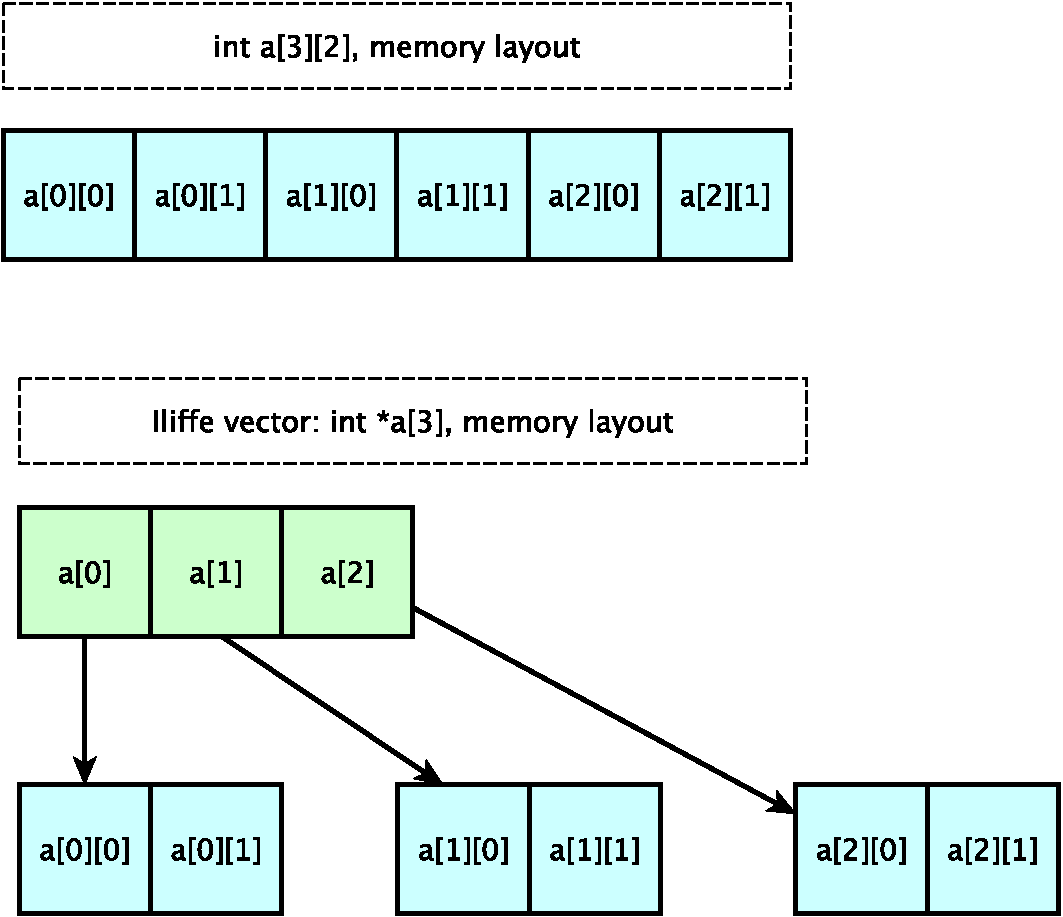
\includegraphics[width=0.8\textwidth]{illustrations/arraylayout-crop.pdf}
\caption{Массивы в языке C}
\label{fig:c_arrays}
\end{figure}

Из-за этого в точке обращения к массиву существует контекстная зависимость -- неясно обращение к чему именно происходит: к jagged-вектору или к одномерному статическому массиву с двумерной адресацией?

\begin{lstlisting}
assert(a[3][4] == *(a + 3*jmax + 4); /* option 1 */
assert(a[3][4] == *(*(a + 3) + 4); /* option 2 */
\end{lstlisting}

Статические массивы в памяти должны всегда быть непрерывны. Для многомерных массивов раскладка в памяти идёт построчно (см. рис. \ref{fig:c_arrays}). При этом последние индексы идут последними. Так же и с инициализацией.

\begin{lstlisting}
float flt[][3] = {{1.0, 2.0, 3.0}, {4.0, 5.0}}; /* ok */
\end{lstlisting}

При этом наиболее вложенные скобки относятся к последним индексам. Первый индекс ясен из контекста и его можно опускать в инициализаторе.

Если часть вложенных инициализаторов пропущена, они считаются нулевыми, поэтому, например двумерные массивы символов могут быть проинициализированы последовательностями строковых литералов.

При передаче многомерных массивов в функции может быть опущен только первый индекс в прототипе (и он может быть любым). Остальные индексы у формального и фактического аргументов должны совпадать.

\textbf{Вопрос к студентам:} возможен ли такой прототип функции?

\begin{lstlisting}
int func(int a[][], int n);
\end{lstlisting}

\ifanswers
Правильный ответ: нет, так как у статического массива не могут быть опущены оба индекса. Допустимы следующие варианты:

\begin{lstlisting}
int func(int a[][3], int n);
int func(int (*a)[3], int n);
\end{lstlisting}
\fi

Точно так же нельзя, даже указав нужные инициализаторы, определить двумерный массив, для которого компилятор дедуцирует оба размера

\begin{lstlisting}
int a[][] = {{1, 2}, {3, 4}}; /* Error! */
\end{lstlisting}

Увы, но здесь, как и в прототипах функций, должны быть указаны все размеры, кроме, может быть, первого.

\textbf{Вопрос к студентам:} в функцию можно передать массив вместо указателя. Можно ли передать двойной массив туда, где ожидается двойной указатель?

\begin{lstlisting}
int func(int **a, int n, int m);
int a[2][3];
func (a, 2, 3); /* wrong! */
\end{lstlisting}

\ifanswers
Но это не работает. Двумерный массив уже не может деградировать к указателю на указатель, а только к указателю на массив (из рисунка \ref{fig:c_arrays} причины должны быть уже очевидны). 
\fi

\textbf{Вопрос к студентам:} есть ли возможность передать двойной массив туда, где ожидается одинарный указатель?

\ifanswers
Ответ: да, есть забавный трюк.

\begin{lstlisting}
int func(int *a, int n, int m);
int a[2][3];
func (&a[0][0], 2, 3); /* ok */
\end{lstlisting}

Но внутри функции это потребует ручного обслуживания такого ``развернутого'' массива.
\fi

\pagebreak
\subsection{От указателей к ссылкам\index{references}}\label{PointersAndRefs}

Очень важной особенностью C++ является введение довольно низкоуровневой, но принципиально новой конструкции – ссылок. Ссылка это альтернативное имя переменной.

\lstinputlisting[firstline=67,lastline=70]{cpp_code/p1s2.cpp}

Каждая ссылка обязательно должна быть инициализирована в точке определения. ``Ссылка сама по себе'' так же как ``нулевая ссылка'' не могут существовать. Указатель сам по себе является местом для хранения данных, ссылка – это просто имя. Поэтому ссылки не нуждаются в явном разыменовании – каждое обращение к ним это уже разыменование. Поэтому различия существенны:

\lstinputlisting[firstline=76,lastline=81]{cpp_code/p1s2.cpp}

\subsubsection{Использование ссылок}

Главный паттерн для использования ссылок это передача по ссылке входных (неизменяемых) аргументов функций, особенно если типы являются жирными:

\begin{lstlisting}
struct T { /* ... */ }

int foo(const T &a);
\end{lstlisting}

Здесь можно использовать и указатель, но тогда в теле функции его придется постоянно разыменовывать, проверять на \lstinline!NULL! и так далее. Ссылка в этом отношении удобней, прозрачней и безопасней.

С другой стороны, передача изменяемых параметров по неконстантным ссылкам -- дело вкуса:

\begin{lstlisting}
int do_r (T &a);
int do_p (T *a);
/* ... */
do_r (b); /* should b be changed? */
do_p (&b); /* b should be changed! */
\end{lstlisting}

Некоторые считают, что это создаёт неоднозначность в точке использования. Другие считают, что указатели также создают неоднозначность между массивом и указателем.

Не стоит передавать по ссылкам небольшие объекты. У подрастающих программистов часто чешется написать нечто вроде:

\begin{lstlisting}
int foo(const int &a);
\end{lstlisting}

Это допустимо, но тут лучше передать \lstinline!a! по значению. Внутри компилятора ссылки обычно реализуются через указатели, которые могут превосходить по размеру небольшие целые. Поэтому тут ваш выбор:

\begin{lstlisting}
int foo(int a);
\end{lstlisting}

Просто и понятно.

Ещё один паттерн использования ссылок -- задание временных имён для безымянных объектов:

\begin{lstlisting}
int &current = big_global_array[calc_index(t)];
current += 1; /* ok, big_global_array changed */
\end{lstlisting}

В этом деле ссылки настолько удобны, потому что по стандарту они продлевают время жизни автоматических переменных:

\begin{lstlisting}
const int &c = a + foo();
/* ... */
use (c); /* ok, c holds temporary value */
\end{lstlisting}

В противовес этому использование в этом контексте указателя создало бы UB.

Здесь const reference binding продляет время жизни временного объекта. Обратите внимание: ссылка связана с временным объектом. При попытке использовать там неконстантную ссылку ничего работать не будет. Зато константная ссылка продляет всё что угодно, даже константу

\begin{lstlisting}
const int &lv = 0; // ok
\end{lstlisting}

Теперь \lstinline!lv! это второе имя для нуля.

\textbf{Вопрос к студентам:} как вы думаете, можно ли вычислить адрес временного объекта на который ссылается \lstinline!lv!?

\ifanswers
Ответ: увы нет и, более того, сам этот объект не обязан существовать.
\fi

\subsubsection{Висячие ссылки}\label{DanglingRefs}

Итак, ссылка это второе имя объекта. Но что если срок жизни объекта истёк?

\begin{lstlisting}
int *t = malloc (sizeof (int) * 10);
int &r = t[2];
free (t); /* end of lifetime */
use (r); /* BOOM */ 
\end{lstlisting}

В этом случае ссылка считается ``повисшей'' (dangling\index{dangling reference}) и любое её использование это UB.

Аналогично ссылка может повиснуть если возвращать из функции ссылку на временный объект. Последний GCC выдает на эту тему warning.

\begin{lstlisting}
int& 
refret (int x)
{
  return x;
}

int &v = refret (3);
cout << v << endl; /* BOOM */
\end{lstlisting}

Здесь тоже всё очень плохо.

\textbf{Вопрос к студентам:} как исправить приведенный выше код и всё-таки вернуть валидную ссылку из функции?

\ifanswers
Ответов может быть много: статические переменные, динамическая аллокация, глобалы, выберите ваш вариант
\fi

\textbf{Вопрос к студентам:} что можно сказать насчёт возврата временного объекта в ссылку по значению?

\begin{lstlisting}
int xret (int x)
{
  return x;
}

const int &lv = xret (1);
\end{lstlisting}

\ifanswers
Правильный ответ: тут всё нормально, работает обсуждавшееся выше расширение срока жизни.
\fi

\subsubsection{Когда ссылки уступают указателям}\label{PointersVsRefs}

В целом при программировании на C++ следует повсюду предпочитать использование ссылок использованию указателей.

Но есть нюансы. Ссылки иммутабельны -- назначив ссылку ``другим именем'' чего-то, её нельзя перевязать на что-то другое

\begin{lstlisting}
int a = 2;
int b = 3;

int *pa = &a; /* ok */
pa = &b; /* ok, now *pa == 3 */

int &ra = a; /* ok */
ra = b; /* ok, now a == 3 */
\end{lstlisting}

Вторая строчка в случае ссылок -- не перевязывает ссылку, а присваивает значение тому lvalue на которое она ссылается. Поэтому ссылки нельзя использовать для создания динамических структур данных, таких как стеки, очереди, деревья.

Кроме того, у ссылок нет аналога \lstinline!(void *)! для передачи идиомы ``ссылки на неопределённый тип''. Появившиеся в новом стандарте \lstinline!auto&! всё таки должны быть разрешены на этапе компиляции, что бывает невозможно:

\begin{lstlisting}
void *read (void);

void 
use (void)
{
  int a = *(int *) read(); /* read int */
  double d = *(double *) read(); /* next read double */
  /* ... */
}
\end{lstlisting}

Итак, использование ссылок должно происходить где это возможно, но нужно хорошо понимать места, в которых их использование невозможно или нецелесообразно.

\pagebreak
\subsection{От программирования в стиле C к программированию в стиле C++}

\hfill\textit{Most people's C programs should be indented}

\hfill\textit{six feet downward and covered with dirt}{\vspace{0.5em}}

\hfill\textit{-- Blair P. Houghton}

C++ имеет много своих идиом. Многие из них на этом этапе могут быть непонятны (зачем заменять такой хороший malloc на этот странный new?) но переход на активное использование этих идиом лучше начинать уже сейчас, а их подлинная сила откроется позже.

\subsubsection{От ввода-вывода через функции к потокам}\label{PrintfToCout}

Все мы знаем (а автор этих лекций так и вообще предпочитает) старые добрые функции, которые в C использовались для вывода. Здесь можно их вспомнить в последний раз тихим ласковым словом. 

Главной структурой, обобщающей ввод-вывод в C является структура \lstinline!FILE! (наследие идеологии Unix, где всё считается файлом, включая такие странные вещи, как консоль или сокет). Поскольку размер этой структуры implementation defined, обычно для совместимости используется \lstinline!FILE*!. Файлы можно создавать, открывать, переоткрывать и закрывать. Количество файлов, которым может оперировать программист задаётся константой \lstinline!FOPEN_MAX! и по стандарту не может быть меньше 8, включая три стандартных файла: \lstinline!stdin!, \lstinline!stdout! и \lstinline!stderr! (первый обычно является read-only и слушает клавиатуру, вторые write-only и направлены на консоль).

Файловый ввод-вывод бывает буферизованным и не буферизованным (традиционно \lstinline!stdout! буферизован, а \lstinline!stderr! нет). Буферизованный вывод накапливает определенное количество символов и только потом выводит его в файл, таким образом уменьшая число обращений к физическим устройствам вывода. С другой стороны, при аварийном завершении программы содержимое буфера может испариться, поэтому в таких сценариях лучше использовать небуферизованный вывод.

Буферизация в свою очередь бывает полной и построчной. Скажем, \lstinline!stdout! буферизован построчно -- вывод конца строки сбрасывает буфер на физическое устройство.

Для открываемых вновь файлов, программист может установить режим буферизации через \lstinline!setvbuf! (C11 7.21.5.6) а также указать собственный буфер любого размера. Очень часто большой буфер в памяти для файла позволяет в разы ускорить работу с ним. Разумеется, в любой момент буфер может быть принудительно сброшен через \lstinline!fflush!.

Ввод и вывод в файлы в языке C бывает форматированный и не форматированный. Базовые функции неформатированного ввода и вывода это \lstinline!fputc! и \lstinline!fgetc!, позволяющие посылать в файл (читать из файла) один символ. Также к базовым относится функция \lstinline!ungetc!, позволяющая временно положить назад символ в файл, доступный на чтение. Гарантируется временное помещение назад одного символа (даже для небуферизованных файлов доступных только на чтение, какой-нибудь там клавиатуры, etc). Это позволяет при необходимости ``забыть'' считанный символ а потом считать его же ещё раз и очень полезно для лексических анализаторов. Чтобы считать таким образом строку символов нужен целый цикл и чтобы избавить от необходимости писать такие циклы, существуют функции \lstinline!fread! и \lstinline!fwrite!. 

Базовый неформатированный hello world приведен ниже.

\begin{lstlisting}
fputs("Hello, world\n", stdout);
\end{lstlisting}

Форматированный ввод и вывод -- самая интересная и спорная часть стандартного вывода. Форматировать можно как вывод в файл (\lstinline!fprintf!), так и вывод в строку (\lstinline!sprintf!). С форматированием, прошлый пример будет иметь вид.

\begin{lstlisting}
fprintf(stdout, "%s\n", "Hello, world");
\end{lstlisting}

К сожалению, такой способ вывода небезопасен относительно типов (компилятор не может проверить форматную строку на соответствие типу аргумента). Он подвержен ошибкам, скажем если передать вместо строчки адрес в памяти, то будет выведено содержимое памяти до первого нулевого символа и так далее. Более того -- нет возможности расширять набор форматных спецификаторов если захочется устроить вывод для своего класса.

В C++ все сишные функции по работе с файлами оставлены, но добавлена новая сущность -- поток ввода/вывода (stream). Эти потоки не стоит путать с потоками исполнения (threads). Поток ввода вывода это не совсем файл, но он может быть основан на файле (\lstinline!fstream!) или на строке (\lstinline!sstream!). Они используются для форматированного ввода или вывода. Стандартные потоки имеют следующее соответствие со стандартными файлами:

\begin{center}
\begin{tabular}{ | l | l | l | }
  \hline
  Тип & Файл & Поток \\ \hline
  Стандартный ввод & \lstinline!stdin! & \lstinline!std::cin! \\
  Стандартный вывод & \lstinline!stdout! & \lstinline!std::cout! \\
  Сообщения об ошибках & \lstinline!stderr! & \lstinline!std::cerr! \\
  Логирование & -- & \lstinline!std::clog! \\
  \hline
\end{tabular}
\end{center}

Неформатированный вывод осуществляется через методы потоков. Например вывод неформатированного Hello, world через write

\begin{lstlisting}
std::cout.write("Hello, world\n", sizeof("Hello, world\n"));
\end{lstlisting}

Форматированный вывод осуществляется через несколько странную конструкцию -- перегруженный оператор сдвига влево (ввод через сдивг справо). Подробнее про перегрузку операторов речь пойдёт дальше (см. \ref{OperatorOverloading}). Пока что стоит отметить, что такая перегрузка операторов -- очень плохая идея (логический сдвиг не имеет отношения к выводу), но исторически устоявшаяся. Для форматирования вывода используются форматные модификаторы.

\begin{lstlisting}
std::cout << "Hello, world" << std::endl;
\end{lstlisting}

Точно так же ввод вывод через потоки может быть буферизован. Потоки ввода-вывода будут рассмотрены подробнее когда речь пойдет про стандартную библиотеку. Пока что может быть неясно (как и со многим в этом разделе) чем они лучше, их подлинная сила вскроется позже.

\subsubsection{От макросов к шаблонным функциям}\label{FunctionTemplate}

Ранее, в разделе (\ref{Inline}) рассматривалось то преимущество, которое даёт C++ (и C начиная с C99) позволяя объявлять встраиваемые функции там, где раньше использовались макросы. Но был указан и недостаток -- отсутствие возможности передавать аргументы любого типа. На самом деле эта возможность есть. Наивный подход иллюстрируется следующим определением функции:

\begin{lstlisting}
template <typename T> inline const T
min (const T a, const T b)
{
  return (a < b) ? a : b;
}
\end{lstlisting}

Говорят, что здесь определен шаблон функции. Синтаксис шаблона ясен из определения: после слова \lstinline!template! в треугольных скобках через запятую перечисляются параметры шаблона. Подробности грамматики изложены в разделе 14 стандарта C++98.

\begin{lstlisting}
template <typename T, class U, int x>
\end{lstlisting}

Здесь слово \lstinline!typename! означает параметр шаблона, задающий имя типа. По историческим причинам можно использовать \lstinline!class!, но новый стандарт поощряет использование \lstinline!typename!. Кроме того вы уже должны видеть в функции \lstinline!max()! существенный недостаток – параметры, передающиеся по значению, в случае увесистого \lstinline!T! будут неэффективны, лучше заменить их константными ссылками.

Подробно шаблонные функции рассматриваются в (\ref{FunctionTemplates}).

\subsubsection{От malloc и free к new и delete\index{new}\index{delete}}\label{newdelete}

Для управления динамической памятью в языке C использовались библиотечные функции \lstinline!malloc! и \lstinline!free!. Они остались в C++, но их использование во многих случаях не рекомендовано и иногда считается дурным тоном, поскольку C++ предоставляет гораздо более гибкие возможности с помощью ключевых слов \lstinline!new!, \lstinline!delete! и \lstinline!delete[]!.

\begin{lstlisting}
struct S {}; 

// Was: t = (struct S*) malloc (sizeof(struct S));
struct S *t = new S; 

// Was: free(t);
delete t; 

// Was: t = (struct S*) malloc (sizeof(struct S) * 5);
struct S *a = new S[5]; 

// Was: free(a);
delete[] a; 
\end{lstlisting}

Следует оговориться, что для C-подмножества эти возможности пожалуй менее гибкие и более ограничивающие. Нужно помнить о парности \lstinline!new!/\lstinline!delete! и \lstinline!new a[]!/\lstinline!delete[] a! и нет возможности сделать \lstinline!realloc!. Вся сила новых ключевых слов раскроется позже, когда будут рассматриваться элементы ООП (см. например \ref{PodNpod}). Пока что можно просто запомнить их и начинать применять. Впрочем и в C-подмножестве можно найти плюсы.

Например, ключевое слово \lstinline!new! существенно упрощает выделение в памяти многомерных массивов, что было не так то просто в случае языка C. Для C++ можно просто записать:

\begin{lstlisting}
typedef int dimensions[3][4];

dimensions * dim = new dimensions[10];
dim[/* 0 to 9 */][/* 0 to 2 */][/* 0 to 3 */] = 42;
delete [] dim;
\end{lstlisting}

Это не требует убогих трюков когда массив выделяется как одномерный, а потом обслуживается как двумерный -- всё прозрачно и типизировано.

\textbf{Вопрос к студентам:} каким образом устроен выделенный таким образом трёхмерный массив в памяти?

\ifanswers
Правильный ответ: это jagged-вектор из одномерных массивов с двумерным доступом к каждому
\fi

Пока что это всё, что можно сказать. Более детальное и углубленное изучение управления памятью предстоит далее, в (\ref{NewMalloc}).

\subsubsection{От приведения в стиле C к приведению в стиле C++\index{cast}}\label{FromCCastToCPP}

Язык C, поскольку он разрабатывался с интенцией отображения один в один на машинные типы, имеет слабую типизацию. Кусок памяти, который хранит int или указатель на int или механическую структуру из чего-нибудь, легко приводится к другому такому же куску памяти.

\lstinputlisting[firstline=95,lastline=100]{cpp_code/p1s2.cpp}

Язык C++ содержит гораздо более развитую систему типов и позволяет определять типы, обладающие состоянием и поведением, о которых пойдёт речь в следующих лекциях. Поэтому, несмотря на то, что формально C++ унаследовал от C способ непосредственного приведения C-style cast, применять его считается крайне плохим тоном. Вместо этого следует применять \lstinline!static_cast!\index{static\_cast}, \lstinline!reinterpret_cast!\index{reinterpret\_cast} или \lstinline!const_cast!\index{const\_cast}. Чаще всего вы будете применять \lstinline!static_cast!. Он записывается так.

\lstinputlisting[firstline=106,lastline=107]{cpp_code/p1s2.cpp}

В принципе это визуально мало чем отличается от C-стиля, рассмотренного выше. Запись чуть более уродлива, зато чуть лучше бросается в глаза в коде программы. Разница в том к чему можно применять \lstinline!static_cast!, а к чему C-cast. Последний применяется к чему угодно. \lstinline!static_cast! применяется только к переменным, совместимым по статическим типам: то есть одинаковым по размеру или указывающим на объекты одинакового размера.

\begin{lstlisting}
float f = 1.0f;
double *d = (double *) &f; // Hmm...
double *e = static_cast<double *>(&f); // CE
\end{lstlisting}

В приведенном примере, компилятор убережет вас от почти неизбежного неопределенного поведения.

Гораздо более редкий \lstinline!const_cast! нужен для снятия константности и волатильности. С его помощью можно привести \lstinline!const int *! к \lstinline!int *!. 

\lstinputlisting[firstline=113,lastline=114]{cpp_code/p1s2.cpp}

Конечно необходимо понимать опасность этих игр: в памяти, выделенной для \lstinline!const int*!, компилятор размещает данные, изменения которых не ожидает. В тот момент, когда программист принудительно снимает константность и изменяет (пытается изменить) нечто, объявленное ранее константным, он стреляет себе в ногу.

И самый редкий \lstinline!reinterpret_cast! существует для непереносимых низкоуровневых приведений, которые, тем не менее, иногда нужны.

\lstinputlisting[firstline=120,lastline=121]{cpp_code/p1s2.cpp}

Любое использование \lstinline!reinterpret_cast! (как и C-cast) компрометирует вашу программу. Но случаи использования \lstinline!reinterpret_cast! читающему ваш код будет куда проще найти и вычистить.

На самом деле, даже \lstinline!reinterpret_cast! чуть лучше, чем C-cast. Потому что C-cast на самом деле делает следующее (C++14 5.4): пробует сверху вниз перечисленные ниже приведения и подставляет то из них, которое подходит.

\begin{itemize}
\item \lstinline!const_cast!
\item \lstinline!static_cast!
\item \lstinline!static_cast! а потом \lstinline!const_cast!
\item \lstinline!reinterpret_cast!
\item \lstinline!reinterpret_cast! а потом \lstinline!const_cast!
\end{itemize}

Это погружение все ниже и ниже. Хуже того, C-cast вообще способен приводить к ещё не определенным типам.

\begin{lstlisting}
struct T; // forward-decl
float f = 1.0f;
T *t = (T *) &f; // (!)
\end{lstlisting}

Разумеется, ни одно из трёх рассмотренных преобразований такого не позволяет.

Выучить и использовать три рассмотренных оператора не намного сложнее, чем использовать обычные преобразования в стиле C, но часто они оказываются крайне полезны, упрощая поддержку кода и не давая посадить тяжело обнаружимых ошибок приведения.

\pagebreak
\subsection{Перегрузка функций, аргументы по умолчанию и искажение имён\index{Function Overloading}\index{Name Mangling}}\label{NameResolution}

\hfill\textit{Необходимо начать с исправления имен}{\vspace{0.5em}}

\hfill\textit{-- Конфуций}

\textbf{Вопрос к студентам:} сколько функций вычисления квадратного корня вы можете назвать из стандартной библиотеки языка C?

\ifanswers
Правильный ответ: три (7.12.7.5) \lstinline!sqrtf!, \lstinline!sqrt! и \lstinline!sqrtl!. Три функции с разными именами понадобилось вводить потому, что они принимают аргументы разных типов, а язык C предоставляет достаточно сильную гарантию того, что любое имя, использованное в вашей программе будет отображено в ассемблер вашей целевой машины один к одному, без искажения.
\fi

Язык C++ такой гарантии не даёт. Вместо этого он согласен сделать эту (и многую другую) работу за вас посредством встроенного искажения (манглирования) имён. Используя C++ вы можете написать три функции с одинаковыми именами, но различными типами:

\lstinputlisting[firstline=125,lastline=127]{cpp_code/p1s2.cpp}

На уровне ассемблера они могут выглядеть например так:

\begin{verbatim}
_Z3barc:
...
_Z3bari:
...
_Z3barx:
...
\end{verbatim}

Конвенции манглирования не документированы и являются implementation-defined, закладываться на них не надо. Но грамотно использовать механизм перегрузки функций в C++ бывает очень выгодно для облегчения читаемости вашей программы.

Для большинства компиляторов C++ существуют ``деманглеры'' -- специальные приложения, способные по искаженному имени ассемблерной метки восстанавливать сигнатуру функции. Скажем в GCC это \lstinline!c++filt!. Попробуйте, скажем: \lstinline!c++filt _ZN4Anls3Cfg7_DeleteEPKv!

Иногда требуется из кода на C++ сделать некую функцию или переменную (обычно входящую в интерфейс модуля) ``линкуемой в C стиле'' -- т.е. отображаемой в ассемблер один в один. Для этого используется спецификатор линковки \lstinline!extern "C"!. Им можно как аннотировать функцию или переменную, так и брать их в блоки.

\begin{lstlisting}
extern "C" void 
foo(int);

extern "C"
{
   void g(char);
   int i;
}
\end{lstlisting}

Так слинкованы могут быть свободные функции и глобальные переменные, но не члены классов. Две функции с такой линковкой с одинаковым именем -- нарушение ODR.

\textbf{Домашняя наработка:} посмотрите как работает манглирование в вашем любимом компиляторе. Можете ли вы установить некие закономерности?

Также удобная концепция (и снова проистекающая от отсутствия обязательств C++ быть близким к машине) это аргументы по умолчанию. Посмотрим как они могут быть заданы:

\lstinputlisting[firstline=1,lastline=5]{cpp_code/p1s2.cpp}

Функция не может быть перегружена по значению аргумента по умолчанию. Для перегрузки вы можете использовать только сигнатуру – возвращаемый тип функции и типы её аргументов.

Перегрузка функций и аргументы по умолчанию сильно упрощают работу с именами функций в C++, перенося всю её тяжесть на плечи компилятора и вам следует научиться использовать эти возможности правильно.

\subsubsection{Правила разрешения перегрузки\index{overloading resolution}}\label{Overloading}

Многие считают, что разрешение перегрузки в C++ неочевидно и подчиняется странным правилам. На самом деле это так и есть. Но вдумчивое чтение стандарта (вся 13 глава посвящена перегрузке) позволяет вывести некоторые закономерности. 

Можно запомнить или записать:

Если среди вариантов перегрузки присутствует функция, точно совпадающая с вызываемой по типам аргументов, будет вызвана она. Далее применяются преобразования аргументов в следующем порядке:

\begin{enumerate}
\item Стандартные преобразования
\item Пользовательские преобразования
\item Троеточия
\item Ссылочное связывание
\item (новый стандарт) Списочная инициализация
\end{enumerate}

После каждого типа преобразований сверху-вниз, получается множество возможных функций. Если это множество состоит из одной функции, будет вызвана она. Если это множество состоит из нескольких функций, будет выдана ошибка компиляции. Если это множество пусто, будет попробован следующий тип преобразований аргументов.

Пока можно оставить за бортом третий и пятый типы преобразований, до них дойдёт дело в своё время. Простой пример на всё остальное:

\begin{lstlisting}
#include <cstdio>

int foo (char x) { return 0;}  /* step 1 */
int foo (short x) { return 1;} /* step 1 */
int foo (int x) { return 2;}   /* step 0 */
int foo (...) { return 3;}     /* step 3 */
int foo (int &x) { return 4;}  /* step 4 */

int
main (void)
{
  std::printf ("result: %d\n", foo (10));
  return 0;
}
\end{lstlisting}

Здесь никаких конфликтов нет. Для вызова \lstinline!foo (10)! точно подходит \lstinline!foo (int)!, программа возвращает 2.
Если стереть её, то будет ошибка компиляции:

\begin{lstlisting}
#include <cstdio>

int foo (char x) { return 0;}  /* step 1 */
int foo (short x) { return 1;} /* step 1 */
int foo (...) { return 3;}     /* step 3 */
int foo (int &x) { return 4;}  /* step 4 */

int
main (void)
{
  std::printf ("result: %d\n", foo (10));
  return 0;
}
\end{lstlisting}

Конфликт между двумя равноправными функциями \lstinline!step 1!. Если далее стереть одну из них:

\begin{lstlisting}
#include <cstdio>

int foo (char x) { return 0;}  /* step 1 */
int foo (...) { return 3;}     /* step 3 */
int foo (int &x) { return 4;}  /* step 4 */

int
main (void)
{
  std::printf ("result: %d\n", foo (10));
  return 0;
}
\end{lstlisting}

Снова всё норм, программа вернёт 0. Если стереть оставшуюся.

\begin{lstlisting}
#include <cstdio>

int foo (...) { return 3;}     /* step 3 */
int foo (int &x) { return 4;}  /* step 4 */

int
main (void)
{
  std::printf ("result: %d\n", foo (10));
  return 0;
}
\end{lstlisting}

Программа вернёт 3. И, наконец, если стереть все варианты кроме ссылочного связывания, программа вернёт 4.

Если вдуматься в эти правила они уже не выглядят столь марсианскими, правда? Хех. Это от того, что я рассказал вам их \textbf{не все}. Тема разрешения перегрузок ещё будет затронута в разговоре про ООП и далее, в разговоре про новый стандарт. Но на уровне C подмножества, всё выглядит довольно логично.

\pagebreak
\subsection{Пространства имён\index{namespaces}}\label{Namespaces}

Каждое объявление в C++ принадлежит некоторому пространству имён. 

\subsubsection{Создание и использование пространств имён}

Глобальное пространство имён это префикс через два двоеточия, а все стандартные функции принадлежат пространству имён std. Напишем hello world с явным указанием пространств имён.

\lstinputlisting[firstline=1,lastline=7]{cpp_code/p1s3.cpp}

Обратите внимание на включение \lstinline!<cstdio>! вместо привычного \lstinline!<stdio.h>! хедера. Все заголовочные файлы к которым вы привыкли в C, сохранены в C++. Но хорошим тоном считается писать унаследованные заголовочные файлы в C++ conforming виде, то есть \lstinline!<cXXX>! вместо \lstinline!<XXX.h>!.

Нужно быть осторожным с теми функциями, которые объявлены в стандартной библиотеке языка C как макросы, а не как функции. Разумеется, макросы не могут быть обернуты никаким пространством имен, поэтому правильно писать \lstinline!assert! а не \lstinline!std::assert!. Макросы в стандартной библиотеке нужны там, где функциональность может быть отключаема -- скажем опция \lstinline!NDEBUG! позволяет сделать сборку более эффективной, отключив все ассерты в приложении. 

Засорять собственными именами, такими как \lstinline!::helloworld!, глобальное пространство имён это на самом деле крайне плохая идея. Несколько лучше объявить своё пространство имён, включив туда всё, что специфично именно для вашей программы.

\lstinputlisting[firstline=1,lastline=9]{cpp_code/p1s4.cpp}

Допустимо объявлять вложенные пространства имён с произвольным количеством уровней вложенности. При помещении в пространство имён функции с большим телом, вполне достаточно поместить в пространство имён явно только объявление (например в заголовочном файле), указав пространство имён при определении (например в файле реализации).

\lstinputlisting[firstline=1,lastline=6]{cpp_code/p1s5.cpp}

Пространства имён являются областями видимости (как блоки из фигурных скобок) и подчиняются тем же правилам – если имя указано в охватывающем пространстве имён оно может быть использовано без квалификации. Но в отличии от блоков скобок они могут быть поименованы и тогда переменная или функция с квалификацией может быть использована где угодно

\lstinputlisting[firstline=8,lastline=17]{cpp_code/p1s5.cpp}

Здесь приведён пример неименованного пространства имён (по русски это звучит странно, лучше говорить ``анонимное пространство имён''). Объявленные в анонимном пространстве имён функции доступны только в текущем модуле -- этим они похожи на функции, объявленные с модификатором \lstinline!static!

В пространстве имён \lstinline!buz! есть доступ к \lstinline!foo::y!. Также можно избежать необходимости постоянно ставить некий префикс (например \lstinline!std::!) если включить это пространство имён в текущее с помощью директивы \lstinline!using!. Этой директивой можно включить и одно имя и целое пространство.

\subsubsection{Поиск Кёнига}

Когда компилятор видит, например, вызов функции, имя этой функции он будет искать:
\begin{itemize}
\item
сначала в области видимости вызова и текущем пространстве имён
\item
далее в пространствах имён аргументов, включая их классы и все базовые классы
\end{itemize}

Этот трюк называется ``поиск Кёнига''\index{Kenig search} по имени человека, который его придумал и ввёл в стандарт C++98.

\lstinputlisting[firstline=19,lastline=28]{cpp_code/p1s5.cpp}

Впрочем, если компилятор встречает вызов фукции внутри метода некоего класса, то иные члены этого класса и его родительских имеют приоритет над функциями, найденными на основании информации о типах аргументов.

В стандарте C++14 добавлены так называемые встраиваемые пространства имён, которые могут по умолчанию включаться в охватывающее пространство (см. \ref{InlineNameSpaces}) но без особой нужды (обсуждаемое там же версионирование и т.п.) лучше обходиться рассмотренными здесь средствами.

Любая стандартная функция в C++ принадлежит пространству имён std. Каждый раз писать \lstinline!std::printf! или \lstinline!std::memcpy! бывает накладно. Чтобы этого избежать, добавьте строчку \lstinline!using namespace std!\index{using} после включения хедеров. Директива \lstinline!using some_name! также может применяться чтобы внести из произвольного пространства имён только одно имя.

\lstinputlisting[firstline=1,lastline=10]{cpp_code/p1s6.cpp}

Поиск Кёнига не срабатывает для имён, которые компилятор считает известными

\begin{lstlisting}
typedef int f;

namespace N {
  struct A;
  int f(A*);
}

int g(N::A *a)
{
  int i = f(a);
  /* f is the typedef, not the N::f
     function: equivalent to int(a) */
  return i;
}
\end{lstlisting}

Без верхнего \lstinline!typedef! всё сработало бы прекрасно, но в его присутствии, компилятор не будет искать функцию \lstinline!f!, полагая, что здесь написано преобразование к типу \lstinline!int!.

Поиск Кёнига также ломается на шаблонных функциях. Особенно это заметно когда не работает вывод типов, например:

\begin{lstlisting}
namespace N {
  struct A;
  template <typename T> int f(A*);
}

int g(N::A *a)
{
  int i = f<int>(a);
  return i;
}
\end{lstlisting}

Здесь поломка обусловлена странностями грамматики языка: имя \lstinline!f! не введено в область видимости как имя шаблонной функции и компилятор считает, что вместо параметризации шаблона записано сравнение на меньше.

Выход: явно ввести имя как имя шаблонной функции:

\begin{lstlisting}
namespace N {
  struct A;
  template <typename T> int f(A*);
}

template <typename T> void f(int);
\end{lstlisting}

Несмотря на другие аргументы, такая функция уже будет кандидатом на перегрузку и запустит поиск Кенига по всем остальным местам.

\subsubsection{Встраиваемые пространства имён}\label{InlineNameSpaces}

Встраиваемые пространства имён позволяют по умолчанию включать символы из помеченного таким образом пространства имён в охватывающее. Похоже на то как это происходит с неименованными пространствами имён из (\ref{Namespaces}), но, благодаря транзитивности, это их свойство может использоваться для замечательных трюков с версионированием.

Например некая библиотека реализует функциональность работы с сетью. Её изначальный интерфейс мог выглядеть следующим обрзом.

\begin{lstlisting}
namespace Networking 
{
  struct TCPSocket;
  struct UDPSocket;
}
\end{lstlisting}

Но потом появилась необходимость поддержать в программе вторую версию \lstinline!TCPSocket!.

\begin{lstlisting}
namespace Networking 
{
    namespace V1 
    {
        struct TCPSocket;
    }
     
    namespace V2 
    {
        struct TCPSocket;
    }
 
    struct UDPSocket;
}
\end{lstlisting}

Увы, такой подход сломает весь пользовательский код этой библиотеки, так как \lstinline!Networking::TCPSocket! должен будет везде быть заменен на \lstinline!Networking::V2::TCPSocket!.

Стандарт C++11 предлагает выход в виде встраиваемого пространства имён, которое неявно включается в охватывающее:

\begin{lstlisting}
namespace Networking 
{
    namespace V1 
    {
        struct TCPSocket;
    }
     
    inline namespace V2 
    {
        struct TCPSocket;
    }
 
    struct UDPSocket;
}
\end{lstlisting}

В этом случае пользователь сможет продолжать использовать структуру \lstinline!Networking::TCPSocket! которая по умолчанию будет разрешена в \lstinline!Networking::V2::TCPSocket!. Также будут работать прямые указания -- \lstinline!Networking::V1::TCPSocket! и \lstinline!Networking::V2::TCPSocket!.

\subsection{Структуры и объединения}

Очень тонкие и сложные вопросы (причем на удивление коварные) при программировании как на C, так и на C++ связаны с объединениями и структурами.

\subsubsection{Объединения и каламбуры}

Изначально объединения были введены в C для экономии места

\begin{lstlisting}
struct VAROBJECT
{
    enum o_t { Int, Double, String } objectType;

    union
    {
        int intValue;
        double dblValue;
        char *strValue;
    } value;
} object;
\end{lstlisting}

Здесь используется одна и та же память для всех трёх возможных типов значений -- подобно тому как одна комната в отеле может использоваться для трёх разных постояльцев. При этом делается предположение, что постояльцы не пересекаются.

Но очень часто на практике их используют для техники, которая называется ``type punning''. Английское слово ``pun'' обозначает специфическую разновидность юмора (примерно соответствует русскому сленговому слову ``прикол''). В русской википедии используется термин ``каламбур типа'' который кажется мне не слишком удачным. Выглядит эта шутка следующим образом: данные записываются в одно поле объединения, а читаются из другого поля. Таким образом типизация нарушается.

\begin{lstlisting}
union a
{
  double d;
  char pch[10]; /* assume 80-bit double */
};

union a u;
u.d = 1.0;
/* use u.pch for per-byte access */
\end{lstlisting}

Долгое время эта техника была некорректной (в C90 явно заявлено UB в таких случаях) и сильно критиковалась. Но все альтернативы были ещё хуже:

\begin{lstlisting}
char pch[10];
*(double *)pch = 1.0; /* aliasing violation */
\end{lstlisting}

Такой код нарушает strict aliasing (\ref{StrictAliasing}) и часто ломает те предположения, которые компиляторы считают себя вправе делать относительно типизации указателей и данных. В отличии от этого, type punning ничего не ломает. Поэтому в C++11 и в C11, type punning в явном виде разрешен.

\subsubsection{Структуры и выравнивание}

Способ, которым компилятор размещает данные в памяти ограничен скоростью обращения к ним на соответствующей архитектуре. На большинстве современных архитектур обращение происходит быстрее если данные \textbf{выравнены}. Выравнивание каждой переменной часто связано с её размером: переменные типа \lstinline!int! должны лежать по адресу (в байтах) кратному четырём, типа \lstinline!short! кратному двум, и так далее.

Это означает, что четыре переменных, объявленных на стеке следующим образом

\begin{lstlisting}
char c1;
int x;
char c2;
short y;
\end{lstlisting}

лягут на условной архитектуре с 32-разрядными указателями примерно так, как показано на (рис. \ref{fig:alignment})

\begin{figure}[h!]
\centering
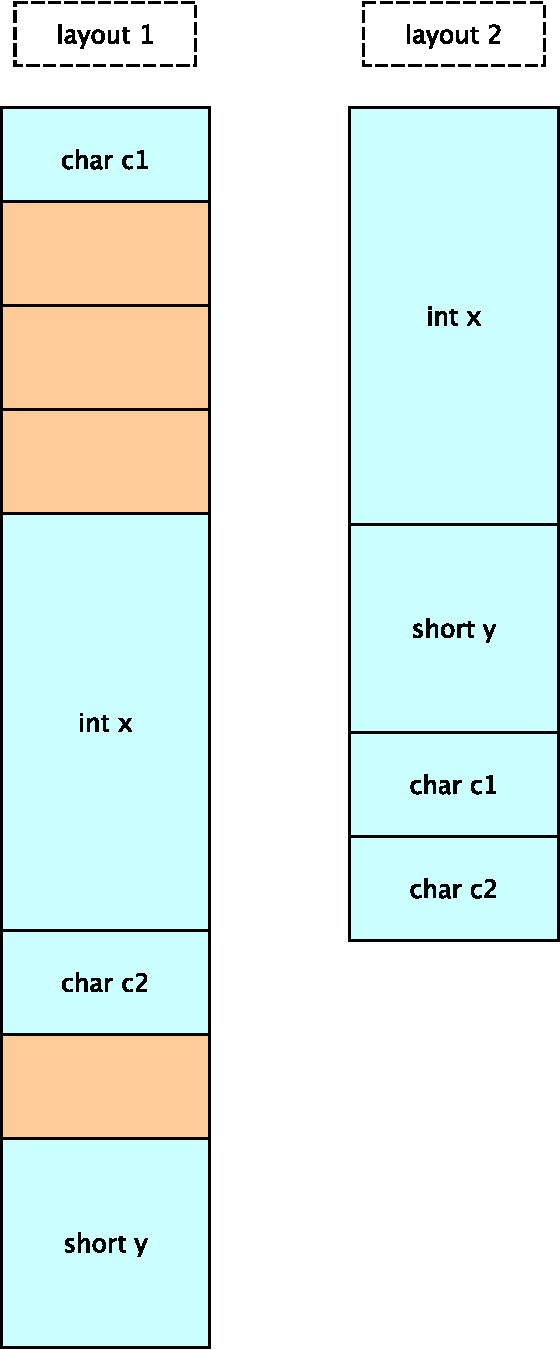
\includegraphics[width=0.4\textwidth]{illustrations/alignment-crop.pdf}
\caption{Два способа выравнивания}
\label{fig:alignment}
\end{figure}

На том же рисунке показано, что простое переупорядочение переменных с учетом выравнивания позволяет сэкономить довольно много места.

Всё то свободное место, которое компилятор оставляет пустым для выравнивания называется заполнителем (padding). В структуре padding обычно идёт между элементами или в самом конце структуры. Например на (рис. \ref{fig:alignment}) заполнители отмечены желтым.

\textbf{Вопрос к студентам:} сколько можно сэкономить на переупаковке вот такой структуры для 32-х битной машины?

\begin{lstlisting}
struct foo
{
  char c;
  char *p;
  short x;
};
\end{lstlisting}

\ifanswers
Правильный ответ: переупаковка в нисходящем порядке

\begin{lstlisting}
struct foo 
{
  char *p;
  short x;
  char c;
};
\end{lstlisting}
\fi

Даст сокращение с 12 до 8 байт. Это уменьшение расхода памяти на 30\% (для массива в котором таких структур сто тысяч такое может быть заметно).

\textbf{Вопрос к студентам:} решите ту же задачу для 64-битной а не 32-битной архитектуры.

\ifanswers
Правильный ответ: теперь указатель будет 8 байт и скоращение с 24 до 16 -- те же 30\%
\fi

Структура как целое также имеет своё выравнивание (обычно оно соответствует наибольшему из требований членов структуры).

\textbf{Вопрос к студентам:} cтудент Шустрый предлагает такое переупорядочение структуры с использованием вложенной структуры

\begin{lstlisting}
struct foo 
{
  struct foo_inner 
  {
    char *p;
    short x;
  } inner;
  char c;
};
\end{lstlisting}

Сколько займет такая структура в памяти 32-х битной машины?

\ifanswers
Ответ: выравнивание внутренней структуры получается 2, а выравнивание внешней структуры 7. Несложный подсчет показывает, что используется целых 16 байт. Немыслимо много. Поэтому с вложенными структурами надо быть осторожней.
\fi

Ещё одна сложность кроется в работе с битовыми полями:

\begin{lstlisting}
struct foo 
{
  int flip:1;
  int nybble:4;
  int septet:7;
  short s;
  char c;
};
\end{lstlisting}

С точки зрения компилятора здесь битовые поля образуют слово, в котором задействованы 12 бит из 16 возможных. В итоге в памяти 32-битной машины, эта структура займет 8 байт. Всё становится гораздо хуже если битовое поле пересекает границу слова.

\begin{lstlisting}
struct foo 
{
  int bigfield:30;
  int septet:7;
  short s;
  char c;
};
\end{lstlisting}

Такая раскладка заставляет компилятор разместить \lstinline!septet! в отдельное машинное слово и структура вырастает до 12 байт, из которых 32 бита уходят на семибитное поле.

\textbf{Вопрос к студентам:} Когда для какой-либо структуры вызывается \lstinline!sizeof!, как вы думаете, он возвращает размер с учётом выравнивания и заполнения или без учёта? И почему.

\ifanswers
Правильный ответ: с учётом. Потому что иначе например не работала бы идиома \lstinline!malloc (sizeof(widget))! -- здесь выделялось бы динамической памяти меньше, чем реально нужно.
\fi

\textbf{Вопрос к студентам:} более хитрый вопрос: а возможно ли вообще написать \lstinline!sizeof_unaligned! в сколь бы то ни было переносимом виде?

\ifanswers
Правильный ответ автору неизвестен. Скорее всего нет, но никто не исключает наличие какого-нибудь особо хитрого трюка.
\fi

Для C90, 6.2.6.1/6 явно гласит, что при записи любого значения в структуру, биты её паддинга принимают unspecified значение. Этот же пункт был унаследован всеми стандартами C и C++.

\textbf{Вопрос к студентам:} рассмотрим структуру

\begin{lstlisting}
struct Padded { int x; char y; };
\end{lstlisting}

В предположении, что \lstinline!sizeof(char) == 1! и архитектура выравнена на 4 байта, какой размер заполнителя она будет иметь?

\ifanswers
Правильный ответ: 3 байта.
\fi

\textbf{Вопрос к студентам:} допустим структура явно заполнена нулями

\begin{lstlisting}
struct Padded p;
memset (&p, 0xDA, sizeof(p));
\end{lstlisting}

Заполнится ли при этом значениями \lstinline!0xDA! её паддинг?

\ifanswers
Верный ответ: да, несомненно.
\fi

\textbf{Вопрос к студентам:} теперь допустим, что некое значение записывается в одно из полей структуры: \lstinline!p.x = 2!. Можно ли теперь полагаться, что в паддинге осталось значение \lstinline!0xDA!?

\ifanswers
Верный ответ: нет, потому что см. выше, при записи в поля, паддинг unspecified.
\fi

\subsubsection{Прокачка перечислений}\label{EnumClass}

Стандартные перечисления хороши, но не без проблем: во-первых они неявно конвертируются в \lstinline!int!, таким образом создавая возможность использовать их не по назначению. Во-вторых они экспортируют имена своих перечислителей в окружающую область видимости, создавая таким образом конфликты имен. В-третьих они не типизированы.

Последнее -- самая мрачная проблема:

\begin{lstlisting}
enum E_MY_FAVOURITE_FRUITS {
    E_APPLE      = 0x01,
    E_WATERMELON = 0x02,
    E_COCONUT    = 0x04,
    E_STRAWBERRY = 0x08,
    E_CHERRY     = 0x10,
    E_MY_FAVOURITE_FRUITS_FORCE8 = 0xFF
};
\end{lstlisting}

Намерение программиста здесь понятно: хочется, чтобы перечислимый тип был восьмибитным. Но каким он окажется в реальности? Это зависит от реализации и тут вполне можно ожидать 32 бит.

Все эти проблемы решает появившаяся в C++11 конструкция \lstinline!enum class!.

\begin{lstlisting}
enum class E_MY_FAVOURITE_FRUITS : 
  unsigned char {
    E_APPLE        = 0x01,
    E_WATERMELON   = 0x02,
    E_COCONUT      = 0x04,
    E_STRAWBERRY   = 0x08,
    E_CHERRY       = 0x10,
    E_DEVIL_FRUIT  = 0x100, // Warning!
};
\end{lstlisting}

Здесь двоеточие используется для указания нижележащего типа. Таким образом компилятор может выдать предупреждение о несоответствии типов, что может спасти много времени в отладке, а программист может сэкономить на размере. 

\pagebreak
\subsection{Автоматический вывод типов}\label{TypeInference}\index{Type inference}

\hfill\textit{Whatever we know without inference is mental}{\vspace{0.5em}}

\hfill\textit{-- Bertrand Russel}

Вывод типов это базовое и очень впечатляющее усовершенствование, которое легко понять и легко использовать. Кроме того, некоторый навык работы с системой типов, в особенности с новыми type traits несомненно нужен для понимания нового стандарта.

\subsubsection{Auto и Decltype}\label{DecltypeAuto}

Одной из главных сильных черт C++ является его сильная типизированность. Тем не менее часто она утомительна. 

\begin{lstlisting}
typedef uint_least8_t decl_handler_t;
decl_handler_t query_resource (int x);
\end{lstlisting}

Теперь каждый раз когда нужно вызвать \lstinline!query_resource!, нужно вспоминать и заводить в программе переменную правильного типа. Или рисковать проблемами, используя для результата \lstinline!int!.

Но казалось бы, компилятор же знает этот тип. Почему его нельзя просто вывести автоматически? В конце концов это работает для шаблонных функций.

\begin{lstlisting}
template <typename T> 
void bar (T x);

bar (query_resource(0));
\end{lstlisting}

Здесь будет сгенерирована по шаблону и вызвана функция \lstinline!bar!, параметризованная типом \lstinline!decl_handler_t!. Начиная с C++11 то же самое можно делать для переменных, заводя для них специальный (автоматический) тип.

\begin{lstlisting}
auto x = query_resource(0);
\end{lstlisting}

Теперь тип переменной \lstinline!x! правильно выводится из реального возвращаемого типа \lstinline!query_resource!, каким бы он ни был.

Если компилятор может взять тип выражения, логично, что это должен уметь и пользователь. Предыдущий кусок кода может быть переписан так:

\begin{lstlisting}
auto i = query_resource(0);
decltype(i) j = i++;
\end{lstlisting}

Здесь на второй строчке объявлено ``сделать j такого же типа, как i''. Это может быть полезно не только для уменьшения кода, но и для облегчения его поддержки:

\begin{lstlisting}
/* maybe in future type of a will change */
void foo (int a)
{
    /* type of b should be type of a */
    decltype(a) b;
    /* do something with b */
}
\end{lstlisting}

Без \lstinline!decltype! можно банально забыть консистентно исправить типы по всей функции и попасть на неприятные и плохо диагностируемые компилятором ошибки при смешивании знаковых и беззнаковых или типов разного размера.

Иногда \lstinline!decltype! может быть сопряжен с некоторыми концептуальными проблемами.

\begin{lstlisting}
struct Point { int x, y; };
Point porig {1, 2};
/* ... */
const Point &p = porig;
decltype(p.x) x; /* int or const int&? */
\end{lstlisting}

\textbf{Тема для обсуждения:} представьте, что вы в комитете по стандартизации. Предложите аргументы в пользу первого и в пользу второго понимания \lstinline!decltype!, проголосуйте.

Это действительно предмет для спора, так как опытный программист может аргументировать и ту и другую позицию. Автор проводил лекции на эту тему и мнения аудитории обычно разделялись в соотношении примерно 60/40 (причем человеческая интуиция работает \textbf{не} в пользу того варианта, который реально принят в стандарте).

Для разрешения этой неоднозначности, стандарт вводит (7.1.6.2) дополнительную форму \lstinline!decltype! с двумя круглыми скобками:

\begin{lstlisting}
decltype(p.x) x; /* int */
decltype((p.x)) x; /* const int& */
\end{lstlisting}

Следует обратить внимание, что, вторая строчка является ошибкой компиляции, так как объявляет неинициализированную ссылку.

На самом деле это различие более тонкое чем просто ещё одни скобки (это была бы слишком грешная магия даже для C++). Речь идёт о разнице между \lstinline!decltype(id-expr)! и \lstinline!decltype((expr))!. Первое возвращает тип, с которым было объявлено имя, второе -- тип, который могло бы приобрести выражение при его вычислении. Как сделать имя выражением? Обернуть его скобками, очевидно. Это кажется некоторым переусложнением, но это на самом деле единственный разумный выход из ситуации. Увы, \lstinline!decltype((expr))! имеет неприятную и с первого взгляда необоснованную особенность -- если тип под ним это lvalue, то он добавит ссылку (если её не было)

\begin{lstlisting}
int x;
typedef decltype(x) xval; /* int */
typedef decltype((x)) xref; /* int& */
typedef decltype((x+1)) xval_again; /* int */

xval r0;
xref r1 = x;
xval_again r2;
\end{lstlisting}

Мотивация для такого поведения станет ясна несколько позже (см. обсуждение в \ref{DeclFunctions}). Но интуитивно это уже ясно -- подчеркивается возможность присваивания. Между прочим выражение ``могло бы быть'' зафиксировано в стандарте и это даёт забавные возможности. Скажем \lstinline!decltype(10000000)! это ``целый тип в котором могло бы поместится 10000000''. Компилятор не обязан выводить наименьший целый тип, но обычно это происходит (в GCC это происходит всегда).

\textbf{Вопрос к студентам:} как насчет \lstinline!decltype((x+y))! если оба \lstinline!int!?

\ifanswers
Правильный ответ: конечно же сумма это не lvalue.
\fi

Вывод типов в C++ работает гораздо более приблизительно, чем их прямая аннотация, поэтому \lstinline!auto! часто выводит первый попавшийся (на самом деле -- наименее общий о чем см. далее) тип, а вот \lstinline!decltype! всегда старается сохранить даже cv-квалификацию

\begin{lstlisting}
  const int s = 5;
  auto s1 = s;
  decltype (s) s2 = 3;
  s1 += 1;
  /* s2 += 1; */
\end{lstlisting}

Строчка \lstinline!auto s1 = 3! ничего не изменит.

Разумное применение этих средств позволяет существенно улучшить читаемость вашего кода и сделать гораздо меньше тонких ошибок и опечаток в сложных именах типов. Но тут нужно учитывать, что всегда есть тонкости и волчьи ямы. Я рассказал как ведет себя \lstinline!auto!, но \lstinline!auto! ведет себя так не всегда. Если вы конкретизируете тип, то все квалификаторы сохранятся вместе с вашей конкретизацией:

\begin{lstlisting}
const int c = 0;
auto& rc = c;
rc = 44; // error: const qualifier was not removed
\end{lstlisting}

Также, и это бывает неприятно, \lstinline!auto! склонно пропускать модификаторы если на верхнем уровне оно встречает то, к чему они относятся:

\begin{lstlisting}
int x = 42;
const int* p1 = &x;
auto p2 = p1; /* p2 is const int* */
p2 = &y; /* ok */
/* *p2 = 3; */
\end{lstlisting}

Язык C++ справедливо считает, что константность данных под указателем это слишком важная характеристика типа. В отличии от этого, константность самого указателя может быть сброшена легко:

\begin{lstlisting}
const int* const p1 = &x;
auto p2 = p1; /* p2 is const int* */
p2 = &y; /* ok */
\end{lstlisting}

Разные правила для \lstinline!decltype! и \lstinline!auto! привели в стандарте C++14 к введению идиомы \lstinline!decltype(auto)! которая позволяет вывести тип из правой части автоматически, но именно так, как его вывел бы \lstinline!decltype!.

\begin{lstlisting}
const int i;
auto j = i; /* typeof(j) == int */
decltype (auto) k = i; /* typeof (k) == const int */
\end{lstlisting}

Очень интересный случай это выражение справа от \lstinline!decltype!, заключенное в круглые скобки.

\begin{lstlisting}
int i;
auto x4a = (i); /* decltype(x4a) is int */
decltype(auto) x4d = (i); /* decltype(x4d) is int& */
\end{lstlisting}

Таким образом моделируется поведение двух круглых скобок у выражения \lstinline!decltype! с конкретным \lstinline!t!.

В качестве вишенки на торте, \lstinline!auto! на самом деле достаточно мощно, чтобы замещать тип во всех контекстах (пример из стандарта C++14 раздел 5.3.4.2)

\begin{lstlisting}
auto x = new auto('a');
\end{lstlisting}

Здесь выведенным значение будет \lstinline!char!. Интересно дальше:

\begin{lstlisting}
auto x1 = { 'a', 'b' };
\end{lstlisting}

\textbf{Вопрос к студентам:} Что будет выведено здесь? 

\ifanswers
Это довольно хитрый вопрос. Ответ ``массив'' неверный. В реальности будет выведен \lstinline!std::initializer_list<char>! -- тот самый новый тип, который позволил так лихо инициализировать вектор в самом начале.
\fi

Интересно, что это -- единственное место, где отличается вывод типов шаблонами (см. \ref{TypeInference}) и \lstinline!auto!. Для шаблонного параметра здесь будет ошибка.

\textbf{Вопрос к студентам:} известно, что в случае обычных типов их можно перечислять через запятую в одном определении. Как вы думаете, какой тип будет выведен здесь?

\begin{lstlisting}
auto x = 5, *y = &x;
\end{lstlisting}

\ifanswers
Вопрос несколько более простодушен. Правильный ответ: увы, это ошибка. Это, правда, создает некоторые проблемы. Неясно почему вот так можно:

\begin{lstlisting}
auto x = 1; 
auto y = 1.0;
\end{lstlisting}

А вот так нельзя:

\begin{lstlisting}
auto x = 1, y = 1.0; /* ! */
\end{lstlisting}

Написано-то как бы одно и то же. Ждем исправления этого в C++17 или более поздних. С другой стороны, жить это не мешает.
\fi

\subsubsection{Расширенный синтаксис функций}\label{DeclFunctions}

Возможности автоматического вывода типов подразумевают построение абстракций с зависимыми типами. Пусть необходим статический шаблонный контракт на любой тип \lstinline!T!, поддерживающий функцию \lstinline!T::makeobject!, возвращающую некий свой тип. Нельзя (по крайней мере в стандарте C++11) просто взять и написать:

\begin{lstlisting}
template <typename T> auto /* Error! */
makeAndProcessObject (const T& builder)
{
    auto val = builder.makeObject();
    /* do stuff with val */
    return val;
}
\end{lstlisting}

Потому что компилятор в точке объявления функции не обладает информацией о типе, который вернет \lstinline!T::makeobject!. Забегая вперед -- иногда обладает, скажем в C++14 тут все хорошо. Точно так же не сработает вот такой выход:

\begin{lstlisting}
template <typename T> 
decltype(builder.makeObject()) /* Error again! */
makeAndProcessObject (const T& builder)
\end{lstlisting}

Потому что \lstinline!builder! не может быть использован до точки своего объявления (которой является список аргументов функции). Конечно правильного прошаренного пацана это не остановит. Он использует тот факт, что значение под \lstinline!decltype! не вычисляется, и сделает тонко:

\begin{lstlisting}
template <typename T> 
decltype (((T*)0)->makeObject()) /* painfull but works */
makeAndProcessObject (const T& builder)
\end{lstlisting}

Но нельзя требовать от программистов такое всерьез, всегда и везде. Комитет по стандартизации решил эту проблему изящно, предложив расширенный синтаксис для обобщённых функций, возвращающих зависимые типы:

\begin{lstlisting}
template <typename T> auto
makeAndProcessObject (const T& builder) -> decltype (builder.makeObject())
{
    auto val = builder.makeObject();
    /* do stuff with val */
    return val;
}
\end{lstlisting}

Внутри скобок \lstinline!decltype! в данном случае вычисление выражения (в том числе вызов функции) не происходит -- происходит только вывод типа.

Выбор правильного результата для гетерогенных функций это большое дело, например:

\begin{lstlisting}
template<typename A, typename B> 
auto add(A const& a, B const& b) -> decltype(a + b) 
{ 
  return a + b; 
}
\end{lstlisting}

Этот подход будет работать во всех случаях, когда входные типы допускают сложение.

Конечно, здесь есть возможные ошибки и засады:

\begin{lstlisting}
template <typename T, typename S>
auto min(T x, S y) -> decltype(x < y ? x : y) 
{
  return x < y ? x : y;
}
\end{lstlisting}

Казалось бы все при всем, но так писать нельзя, поскольку \lstinline!decltype! вокруг выражения работает как \lstinline!decltype(expr)!, а значит результат может быть выведен как ссылка, что чревато. Так как же все таки правильно написать type-generic minimum? Эта проблема найдет свое решение позже (см. \ref{ReferenceConvolution}).

\textbf{Вопрос к студентам:} Представим, что \lstinline!T! и \lstinline!S! это простые типы без квалификаций, указателей ссылок и прочего добра. Просто  \lstinline!int!, \lstinline!double! и всё такое. В каких случаях  \lstinline!decltype! здесь выведет ссылку, а в каких нет? 

\ifanswers
Правильный ответ: ссылка будет если типы одинаковые. Если они разные, все будет хорошо.
\fi

Зато теперь можно понять почему же такое поведение \lstinline!decltype(expr)! было выбрано комитетом по стандартизации. Рассмотрим упрощенную задачу -- допустим речь идет о выводе типа для доступа к элементу массива:

\begin{lstlisting}
template <typename T>
auto array_access(T& array, size_t pos) -> decltype(array[pos]) 
{
  return array[pos];
}
\end{lstlisting}

С текущим подходом можно использовать такую обертку прозрачно как если бы это действительно был доступ к элементу массива:

\begin{lstlisting}
std::vector<int> vect = {42, 43, 44};
int* p = &vect[0];

array_access(vect, 2) = 45;
array_access(p, 2) = 46;
\end{lstlisting}

В противном случае пришлось бы идти на разнообразные хаки.

Позвольте еще маленькую вишенку на этот тортик:

\begin{lstlisting}
auto main() -> int
\end{lstlisting}

Теперь является легитимной формой функции \lstinline!main! и если вы хотите показать насколько вы круче остальных людей в этом мире, то вы теперь знаете, что делать.

Впрочем, это так, отвлечение. Последний стандарт привнес ещё больше радости.

\subsubsection{Коррективы в вывод типов для C++14}\label{DecltypeAuto14}

В некоторых простых случаях компилятору действительно не составляет проблем вывести тип функции: 

\begin{lstlisting}
auto isquare (int x) -> decltype (x) 
{ 
  return x*x;
}
\end{lstlisting}

Здесь указание \lstinline!decltype! выглядит просто излишним и C++14 разрешает его убрать:

\begin{lstlisting}
auto isquare (int x) { return x*x; }
\end{lstlisting}

Для таких простых вариантов все хорошо, но как быть с рекурсией? Здесь возникает проблема: тип должен быть выведен до того, как рекурсивный вызов произошел:

\begin{lstlisting}
auto sum_to (int i)
{
  if (i < 2)
    return i; // return type deduced as int
  else
    return sum_to (i-1) + i;  // ok to call it now
}

cout << sum_to (10) << endl;
\end{lstlisting}

Но если переставить возвраты в вышеприведенном коде, он не будет скомпилирован.

\begin{lstlisting}
auto bad_sum_to (int i)
{
  if (i > 2)
    return bad_sum_to (i-1) + i;
  else
    return i;
}
\end{lstlisting}

Впрочем GCC 4.9.2 возвращает вполне человечное описание ошибки:

\begin{verbatim}
error: use of ‘auto bad_sum_to(int)’ before deduction of ‘auto’
     return bad_sum_to (i-1) + i;
\end{verbatim}

Увы, как уже было сказано \lstinline!auto! режет типы. 

\begin{lstlisting}
auto Example(int const& i) 
{ 
    return i; 
}
\end{lstlisting}

Здесь возвращаемый тип \lstinline!int!. Конечно, в конкретном коде несложно вернуть квалификацию типа:

\begin{lstlisting}
auto const& Example(int const& i) 
{ 
    return i; 
}
\end{lstlisting}

Но что делать в обобщенном коде?

В обобщенном коде для точного вывода возвращаемого типа может быть использован \lstinline!decltype (auto)! например так:

\begin{lstlisting}
template <typename Fun, typename Arg>
decltype(auto) example(Fun fun, Arg arg) 
{ 
    return fun(arg); 
}
\end{lstlisting}

Теперь тип возвращаемого значения будет проброшен точно. Ниже будет показано как написать совершенно прозрачную обертку: пробросив не только возвращаемое значение но и произвольные аргументы (см. \ref{PerfectForw}).

В новом стандарте также нет проблем с тем, чтобы шаблонные методы выводили свой тип непосредственно из других методов того же класса без явного \lstinline!this! (пример взят из стандарта C++14, 5.1.1.3)

\begin{lstlisting}
struct A 
{
  char g();
  template <class T> auto f(T t) -> decltype(t + g())
  { return t + g(); }
};
\end{lstlisting}

\subsubsection{Параметры функций и обобщения для C++17}\label{DecltypeAuto17}

Несмотря на то, что до 2017-го ещё далеко, GCC уже поддерживает как расширения некоторые

\textbf{Вопрос к студентам:} Как вы думаете, какой тип будет выведен здесь: 
\begin{lstlisting}
auto 
foo (auto x = 1) /* note default argument value */
{
  return x;
}
\end{lstlisting}

\ifanswers
Правильный ответ: этот код не должен вводить вас в заблуждение: тип для \lstinline!x! выводится из типа в точке вызова, а не из аргумента по умолчанию
\fi

Это вообще-то не должно работать в C++14, но в GCC 5.2 это будет работать точно так же, как если бы вы написали:

\begin{lstlisting}
template <typename T> auto 
foo (T x = 1) /* now it is obvious that T is not deduced from 1 */
{
  return x;
}
\end{lstlisting}

Это сделано в качестве предложения по концептам в новом стандарте и имитирует то, как это устроено для полиморфных лямбд (см. \ref{GenericLambdas}).

Конечно, до принятия нового стандарта лучше не использовать такие возможности.

\subsubsection{Decaying и минимальные общие типы}\label{Decaying}\index{Decay function}

Decaying уже был рассмотрен, при рассмотрении деградации массивов в указатели (\ref{ArrDecaying}), но если в старом стандарте это была built-in особенность для одной конкретной пары типов, то новый стандарт предлагает интересные варианты обобщения этого понятия на любые типы. Простой случай:

\begin{lstlisting}
int foo (const int &s)
{
  return s + 2;
}
\end{lstlisting}

Здесь в выражении \lstinline!s + 2!, \lstinline!s! ведёт себя так, как будто его тип \lstinline!int!. Тогда можно сказать, что \lstinline!const int &! деградирует к \lstinline!int! в том же смысле, в каком массив деградирует к указателю, etc. Новый стандарт позволяет вручную ``деградировать'' тип:

\begin{lstlisting}
const int &i;
std::decay<decltype(i)>::type j; /* int j */
/* and btw */
auto k = i; /* int k = i; */
\end{lstlisting}

Автоматический вывод также осуществляет деградацию типов. Поэтому можно считать \lstinline!decay! + \lstinline!decltype! способом вывести тот тип, который вывело бы \lstinline!auto!.

На механизме \lstinline!decay! неявно построен механизм \lstinline!common_type!, позволяющий вывести минимальный общий тип:

\begin{lstlisting}
template <typename T, typename S>
void foo(T lhs, S rhs) {
{
  std::common_type<decltype(lhs), decltype(rhs)>::type k;
  // ...
}
\end{lstlisting}

В принципе минимальные общие типы не так уже и нужны

\begin{lstlisting}
template <typename T, typename S>
void foo(T lhs, S rhs) {
  auto prod = lhs * rhs;
  //...
}
\end{lstlisting}

Устроит не менее качественную деградацию. Мало того, такое расширение GCC давно известное и во многих других компиляторах как \lstinline!typeof!, позволяло делать это и в старом стандарте. В новом же можно использовать \lstinline!decltype!.

\begin{lstlisting}
typedef typeof(lhs * rhs) product_type;
typedef decltype(lhs * rhs) product_type;
\end{lstlisting}

В качестве полезного примера, можно привести смешанную арифметику для числового класса:

\begin{lstlisting}
template <typename T>
struct Number { T n; };
 
template <typename T, class U>
Number<typename std::common_type<T, U>::type> 
operator+(const Number<T>& lhs,
          const Number<U>& rhs) 
{
    return {lhs.n + rhs.n};
}
 
int main()
{
    Number<int> i1 = {1}, i2 = {2};
    Number<double> d1 = {2.3}, d2 = {3.5};
    std::cout << "i1i2: " << (i1 + i2).n 
              << "\ni1d2: " << (i1 + d2).n 
              << "\nd1i2: " << (d1 + i2).n 
              << "\nd1d2: " << (d1 + d2).n 
              << '\n';
}
\end{lstlisting}

\textbf{Домашняя наработка:} проанализировать вывод этой программы и то, почему он ведет себя именно так.

\subsection{Мелкие отличия C-подмножества C++ от ISO C}\label{LittleDivergences}

\begin{itemize}
\item
Функция \lstinline!main()! в C++ не может быть вызвана из пользовательского кода. В языке C это разрешено, хотя и несколько необычно.
\item
Прототипы функций обязательны в C++, но опциональны в C.
\item
Сложная и развитая система инициализации в C обычно не работает в C++

\begin{lstlisting}
struct T {
    union {
        struct {
            int x, y, z;
        };
        int xyz[3];
    };
    int a;
};

struct T v = { { .x = 1, .y = 2, .z = 3}, 4 };
struct T w = { { .xyz[0] = 1, .xyz[1] = 2, .xyz[2] = 3}, 4 };
struct T x[] = { [0].a = 1, [1].a = 2 };
\end{lstlisting}

Такой код инициализации легален в C и совершенно нелегален в C++
\item
Имена, определяемые через \lstinline!typedef! не могут совпадать с существующими именами структур в C++, но могут в C (последний требует явной квалификации \lstinline!struct!).
\item
При присвоении к \lstinline!void *! указателю указателя на иной тип, C++ требует приведения (C не требует, но оно считается хорошим тоном).
\item
C++ вводит более десяти новых ключевых слов. Они могут быть использованы как идентификаторы в программе на C, но компилятор C++ выдаст ошибку.
\item
В языке C++ объявление переменной может появится везде, где может быть выражение; в C, объявления должны быть в начале блока.
\item
Имя структуры или объединения во внутренней области видимости скроет такое же имя любой переменной во внешней области видимости в C++, но не в C.
\item
У символьных литералов тип char в C++, но тип int в C. То есть \lstinline!sizeof('a')! даёт 1 в C++, но может дать большее значение в C.
\end{itemize}

\pagebreak
\subsection{Домашняя наработка по базовому C++}

\textbf{Контрольные вопросы} 

\begin{enumerate}
\item Запишите волатильный указатель на массив целых чисел
\item Приведите пример когда использование typedef серьёзно улучшает читаемость кода
\item В каких случаях программист на C++ вынужден пользоваться макросами?
\item В чем преимущество констант над перечислениями?
\item Возможна ли инлайн-подстановка нестатической функции, определенной в другой единице трансляции?
\item В каких случаях вызов функции вместо подстановки идентичного макроса ускоряет работу кода?
\item Может ли объявление структуры располагаться внутри определения функции?
\item Может ли время жизни объекта заканчиваться раньше достижения границ его области видимости?
\item Можно ли использовать ссылку на неполный тип в определении функции?
\item Может ли вызов функции быть lvalue?
\item Можно ли вычислить побитовое или двух указателей?
\item Возможно ли иметь в программе массив из ссылок?
\item Возможна ли ссылка на массив?
\item Всегда ли можно получить указатель на нечто, на что существует ссылка?
\item В каких случаях нельзя заменить static cast на const cast?
\item Может ли функция быть перегружена по cv-квалификатору аргумента?
\item Можно ли расширить пространство имен, определяемое структурой?
\item Есть ли разница в выводе типа auto из правой части или правой части в дополнительных скобках?
\item Можно ли использовать auto в полях структур?
\item Какой тип будет выведен для пустой строки?
\item Какие преимущества имеет новый синтаксис объявления функций?
\item Какой тип является минимально общим между ссылкой на int и ссылкой на float?
\end{enumerate}

\textbf{Задания} 

\begin{enumerate}
\item
Дана структура данных, воплощающая простой односвязный список

\begin{lstlisting}
typedef struct list_tag
{
  void *data;
  struct list_tag *next;
} list_t, *list_p;
\end{lstlisting}

У последнего элемента \lstinline!next = 0!

Необходимо написать на языке C++ функцию, берущую на вход указатель на голову списка и переворачивающую список в памяти, так, что первый элемент становится последним, второй предпоследним и так далее.

\item
Дана программа на языке C с комментариями вида \lstinline!/* comment */!

Необходимо написать на языке C++ программу, выкидывающую все комментарии из текста данной.

\item
Дана структура данных, соответствующая n-арному дереву

\begin{lstlisting}
typedef struct tree_tag
{
  void *data;
  struct tree_tag *top;
  struct tree_tag **childs;
} tree_t, *tree_p;
\end{lstlisting}

Реализуйте на языке C++ функцию, берущую на вход пару указателей на произвольные элементы дерева, и подсчитывающую расстояние между ними (минимальный путь в дереве). Как вы будете тестировать эту функцию?

\item
Реализуйте на языке C++ алгоритм из (\ref{AlgDecl}) и протестируйте на нескольких сотнях сгенерированных определений

\item
Реализуйте на языке C++ транспонирование двумерной матрицы

\item
Реализуйте на языке C++ операцию получения двумерной матрицы обратной данной

\item
Реализуйте на языке C++ операцию умножения вектора на матрицу

\item
Реализуйте на языке C++ калькулятор, делающий вычисления в обратной польской нотации. Например \lstinline!1 2 3 4 + * + =! должно выдавать 25 в качестве результата.

\item
Известны год, месяц и день рождения человека. Реализуйте на языке C++ программу, определяющую его возраст в днях на текущую дату.

\item
Реализуйте на языке C++ программу, подсчитывающую количество лет в 20-м веке у которых первым днём было воскресенье

\item
На вход дана строка из \lstinline!N*N! символов. Реализуйте на языке C++ функцию, выделяющую в памяти двумерную матрицу \lstinline!N*N! и заполняющую её последовательными данными из входной строки.

\item
На вход даны завершающаяся нулём строка \lstinline!haystack! и завершающаяся нулём строка \lstinline!needle!. Реализуйте на языке C++ функцию, определяющую, является ли \lstinline!needle! подстрокой \lstinline!haystack!

\item
В условиях предыдущей задачи необходимо доработать функцию, чтобы она выкидывала из \lstinline!haystack! все вхождения \lstinline!needle! и возвращала измененную строку.

\item
Напишите на C++ программу, которая будет возвращать номер в последовательности Фибоначчи первого числа имеющего 1000 разрядов в десятичном представлении.

\end{enumerate}

\pagebreak
\section{Объектно-ориентированное счастье}

\hfill\textit{I made up the term 'object-oriented',}

\hfill\textit{and I can tell you I didn't have C++ in mind} {\vspace{0.5em}}

\hfill\textit{-- Alan Kay, OOPSLA '97}

Как известно, самой целью создания C++ Бьёрном Строструпом было добавление объектно ориентированных возможностей к C, поэтому изначально язык назывался ``C с классами''. Известно также, что Строструп вдохновлялся языком Simula, но сейчас уже нельзя оценить насколько это была удачная идея, поскольку этот язык канул в лету (зато известна вынесенная в эпиграф цитата одного из гуру ООП). Так или иначе, но C++ действительно обладает уникальной среди современных объектно ориентированных языков моделью объявления и инстанциирования классов. Многим нравится богатство и гибкость её возможностей, многие в ужасе отползают. Эта глава посвящена особенностям ООП в C++ и является центральной темой первого семестра обучения.

\subsection{Структуры в C и в C++}\label{CCppStructs}

В языке C структура являлась способом ввести пользовательский тип, являющийся механическим объединением разнородных данных:

\begin{lstlisting}
typedef struct pair 
{ 
  int x; 
  int y; 
} pair_t;
\end{lstlisting}

\textbf{Вопрос к студентам:} что за странный \lstinline!typedef!, зачем он нужен?

\ifanswers
Правильный ответ: это стандартная идиома, чтобы в коде на C не писать лишний раз \lstinline!struct pair! в два слова.
\fi

Можно написать функцию, создающую обратную пару:

\begin{lstlisting}
pair_t 
transpose_pair(const pair_t *pthis)
{
  pair_t pr = {pthis->y, pthis->x};
  return pr;
} 
\end{lstlisting}

\textbf{Вопрос к студентам:} обоснована ли здесь передача по указателю?

\ifanswers
Правильный ответ: на грани. Указатель может занимать больше места, чем два целых, может и меньше.
\fi

Вызвать эту функцию тоже несложно:

\begin{lstlisting}
pair_t p = {2, 3};
pair_t t = transpose_pair (&p);
assert ((p.x == t.y) && (p.y == t.x));
\end{lstlisting}

Такие типы возможны и в C++. Но в C++ была также добавлена принципиально новая возможность группировать данные с методами их обработки внутри структуры:

\begin{lstlisting}
struct pair_t 
{ 
  int x; 
  int y;
  pair_t transpose_pair (); 
};

pair_t 
pair_t::transpose_pair ()
{
  pair_t pr = {this->y, this->x};
  return pr;
} 
\end{lstlisting}

Здесь следует обратить внимание на то, что в C++ была исключена необходимость добавлять \lstinline!struct! к символьному имени структуры, что делает ненужным оставшийся в C-style коде \lstinline!typedef! тэга структуры на её имя.

Вызов будет выглядеть чуть иначе:

\begin{lstlisting}
pair_t p = {2, 3};
pair_t t = p.transpose_pair ();
assert ((p.x == t.y) && (p.y == t.x));
\end{lstlisting}

Имя метода \lstinline!transpose_pair! структуры \lstinline!pair_t! в C++ также будет манглировано (см. \ref{NameResolution}) и в ассемблере встретится, например, в виде:

\begin{verbatim}
_Z14transpose_pair4pair:
\end{verbatim}

Определённая так функция называется функцией-членом (member function)\index{member function}, а также методом структуры. Объявление метода происходит внутри определения структуры, определение метода имеет явную квалификацию того к чему метод относится. Обратите внимание, что символ сдвоенных двоеточий такой же, как и в случае пространств имён. Он дословно означает ``пространство имён, задаваемое структурой''.

Ключевое слово \lstinline!this!\index{this} обозначает неявный (всегда первый) аргумент в методе класса и является указателем на экземпляр структуры, для которой он вызывается. Поэтому \lstinline!this->y! это поле \lstinline!p.y! при вызове \lstinline!p.transpose_pair()! но это будет уже \lstinline!t.y! при вызове \lstinline!t.transpose_pair()!

По умолчанию \lstinline!this! можно опускать, чтобы не загромождать код. Имена полей класса всё равно являются идентификаторами из наиболее охватывающего пространства имён. Поэтому следующий код является и законным и совершенно эквивалентным приведенному выше:

\begin{lstlisting}
pair_t 
pair_t::transpose_pair ()
{
  pair_t pr = {y, x};
  return pr;
} 
\end{lstlisting}

Такой подход делает появление имён \lstinline!x! и \lstinline!y! в теле метода несколько неожиданным, поэтому многие авторы книг по хорошему стилю рекомендуют выделять название полей. Саттер и Александреску \cite{sutteralexandresku} рекомендуют \lstinline!x_! и \lstinline!y_!, но на практике часто встречаются \lstinline!m_x! и \lstinline!m_y!. В общем это дело вкуса.

\textbf{Вопрос к студентам:} можно ли вызвать метод класса так, чтобы \lstinline!this! был нулевым указателем?

\ifanswers
Правильный ответ: да, через явное приведение типов. Но лучше так не делать, это UB.
\fi

\pagebreak
\subsection{Инкапсуляция и игра в мячик}\label{Encapsulation}

\hfill\textit{I find OOP philosophically unsound.}

\hfill\textit{It claims that everything is an object.}

\hfill\textit{Even if it is true it is not very interesting.} {\vspace{0.5em}}

\hfill\textit{-- Alex Stepanov}

Пусть стоит задача разработать тип данных, который будет использован для моделирования полёта материальной точки в двумерном мире (высота, длина). Мяч может лететь свободно, для чего у него вызывается метод \lstinline!fly(double t)! или его можно толкнуть, придав ему определённую скорость под определённым углом (после чего например опять отправить в полёт и так далее). Можно написать определение структуры, вроде приведенного ниже.

\lstinputlisting[firstline=14,lastline=23]{cpp_code/p2s1.cpp}

Представляет ли эта структура данных хорошую абстракцию мяча? Нет, не представляет. Каждый пользователь вашего ``мяча'' может произвольно менять его координаты. Это означает, что в плохо отлаженной программе симуляции, этот мяч сможет свободно ``телепортироваться'', а это явно не то, чего ждут от законченной модели. 

\lstinputlisting[firstline=29,lastline=36]{cpp_code/p2s1.cpp}

Хуже того, время может быть свободно переставлено вперёд или назад. Но пусть даже никто не ошибся и всё написано правильно. А потом... возникла необходимость ``запустить'' этот мяч в многопользовательской среде. Всё пропало – для того, чтобы вставить синхронизацию, переписывать придётся каждый участок кода где ссылались на эти поля.

\subsubsection{Конкретные классы}\label{ConcreteClasses}

Для разграничения состояния модели от её поведения и более гибкого управления поведением, в C++ были введены классы. Простые классы, без использования полиморфизма и без иерархий наследования, называются ``конкретными классами''. Конкретные классы -- мощный и полезный инструмент для поддержания консистентности абстракции. Можно переписать модель мяча, создав его класс

\lstinputlisting[firstline=43,lastline=54]{cpp_code/p2s1.cpp}

Модификатор \lstinline!public! означает, что любой пользователь типа \lstinline!ball_t! имеет доступ к этим методам или данным. 

Модификатор \lstinline!private! означает, что доступ к соответствующим методам и данным имеют только методы этого класса.

\lstinputlisting[firstline=58,lastline=74]{cpp_code/p2s1.cpp}

Хорошим тоном считается закрывать данные, составляющие состояние объекта и открывать функции, составляющие его поведение.

\subsubsection{POD и NPOD типы}\index{POD}\index{NPOD}\label{PodNpod}

В языке C со структурами всё было довольно просто.

Из-за скрытия состояния и наличия нетривиального поведения, в языке C++ существует ряд категорий типов: типы со специальным созданием, со специальным поведением при копировании, с неизвестным или зависящим от реализации размером и так далее.

Стандарт определяет следующие термины (C++14, 9 раздел) для обозначения категорий типов, объекты которых могут быть созданы.

\begin{itemize}
\item \textbf{Тривиально копируемый} -- тип, непрерывный в памяти и не обладающий специальным поведением при копировании. Для таких типов работает \lstinline!memcpy! и \lstinline!memmove! 
\item \textbf{Тривиальный} -- тривиально копируемый тип без специального поведения при создании.
\item \textbf{Со стандартным расположением полей} -- тип, без зависящих от реализации полей (например без членов-ссылок, без таблиц вирутальных методов и так далее). Такие типы удобны для передачи в модули, написанные на других яызках программирования, например на C или Java -- их всегда можно десериализовать независимым от языка и компилятора образом.
\item \textbf{POD} -- от plain old data -- тривиально копируемый тип со стандартным расположением полей.
\end{itemize}

Все типы, не являющиеся POD называются NPOD (от not plain old data).

По мере введениях новых техник ООП, будет рассмотрено каким становится тип в зависимости от объявления.

Типы с закрытой частью остаются тривиально копируемыми.

\subsubsection{Инициализация и уничтожение\index{constructor}\index{destructor}}\label{ConstrDestr}

Отсутствие доступа к состоянию означает, что при создании объекта он должен уметь сам установить своё состояние, а при уничтожении – освободить свои ресурсы. Для этого в класс вводятся конструктор и деструктор – специальные функции, вызывающиеся при создании и уничтожении объекта. Например у класса мяча, конструктор может устанавливать начальное положение, деструктор же может быть тривиальным.

\lstinputlisting[firstline=18,lastline=21]{cpp_code/p2s2.cpp}

Обратите внимание на список инициализации у конструктора в этом примере кода. Можно, конечно, написать инициализацию в теле конструктора, но использование списков инициализации является лучшей идеей. По умолчанию, удовлетворяющий стандарту языка C++ компилятор сгенерирует конструктор (на самом деле несколько конструкторов) и деструктор по умолчанию. Это кажется удобным, но в \ref{RAII} последует обсуждение того, чем это может быть чревато. Конструктор по умолчанию вызывает конструкторы всех членов класса, у которых они есть, деструктор -- их деструкторы.

\subsubsection{Дополнения в инициализацию и уничтожение}\label{ConstrDestrAddition}

Очень часто масса конструкторов в классе делает одно и то же или почти одно и то же. В этих случаях, начиная с C++11, конструкторы можно \textbf{делегировать} -- то есть вызвать конструктор того же класса из списка инициализации.

Делегация конструкторов

\begin{lstlisting}
    class X {
        int a;
    public:
        X(int x) : a(x) { /* ... some logic ... */ }
        X(double x) : X{static_cast<int>(x)} { }
    };
\end{lstlisting}

Во многих случаях, инициализация списком утомительна. Для того, чтобы сократить записи списков инициализации, была придумана инициализация в теле класса.

\begin{lstlisting}
 class A {
    public:
        A() {}
        A(int a_val) : a(a_val) {}
        A(D d) : b(g(d)) {}
        int a = 7;
        int b = 5;  
    };
\end{lstlisting}

Она так же доступна начиная с C++11 и её очень хорошо использовать чтобы точно не оставить ни одного поля в неинициализированном состоянии.

\subsubsection{Неявное преобразование типов и explicit}\label{Explicit}

Важная тема в конструкторах это их использование для задания неявного преобразования типа\index{implicit type cast}. Неявные преобразования есть и в C, там они называются type promotions, некоторые из них (действуют и в C++) сведены в таблицу ниже (здесь anytype это любой встроенный тип, совместимый по операции но не перечисленный выше):

\begin{lstlisting}
anytype `op` long double => long double `op` long double
anytype `op` double => double `op` double
anytype `op` float => float `op` float
anytype `op` unsigned long long => unsigned long long `op` unsigned long long
anytype `op` long long => long long `op` long long
anytype `op` unsigned long => unsigned long `op` unsigned long
anytype `op` long => long `op` long
anytype `op` unsigned int => unsigned int `op` unsigned int
anytype `op` int => int `op` int
\end{lstlisting}

Но в C++ неявные преобразования также пробуются компилятором для пользовательских типов. Определение в пользовательском типе конструктора, который может быть истрактован как конструктор с одним аргументом (считая аргументы по умолчанию частично подставленными всюду кроме первого аргумента), считается определением неявного преобразование из аргумента конструктора к этому типу. Это может иметь неприятные последствия:

\lstinputlisting[firstline=26,lastline=31]{cpp_code/p2s2.cpp}

Верный способ определить конструктор, чтобы явно заявить компилятору, что он не поддерживает неявного преобразования это определить его с ключевым словом \lstinline!explicit!

\lstinputlisting[firstline=12,lastline=13]{cpp_code/p2s3.cpp}

Это важное решение при проектировании и его надо принимать осознанно. Лепить \lstinline!explicit! куда ни попадя -- дурной тон (скажем это ключевое слово возможно но совершенно не нужно на конструкторе более чем с одним аргументом и без аргументов по умолчанию). Но иногда он очень нужен.

\subsubsection{Value-инициализация и Default-инициализация}\label{ValDefInit}

Тривиальные и нетривиальные типы требуют разной обработки во время выделения памяти. Когда пользователь пишет

\begin{lstlisting}
int *t = new int; /* t uninitialized */
int *pt = new int [10]; /* pt[.] uninitialized */
\end{lstlisting}

Он не ожидает, что будет вызвано десять конструкторов для целых чисел. Вместо этого ожидаемое поведение это десять неинициализированных объектов.

\begin{lstlisting}
struct SomeTriv
{
  int x;
};

SomeTriv *px = new SomeTriv; /* x uninitialized */
\end{lstlisting}

Аналогично никакого конструктора не будет вызвано и в этом случае. Но немного изменим структуру:

\begin{lstlisting}
struct SomeNTriv
{
  int x;
  ~SomeNTriv() {;}
};

SomeNTriv *px = new SomeNTriv; /* x initialized with 0 */
\end{lstlisting}

Поскольку в этой структуре есть деструктор, она теперь не тривиальна и для неё будет сгенерирован конструктор по умолчанию. Для того, чтобы сделать у тривиальных типов такое же поведение, разработчики языка предусмотрели указание пустых скобок для value-initialization:

\begin{lstlisting}
struct SomeTriv
{
  int x;
};

SomeTriv *px = new SomeTriv (); /* x initialized with 0 */
int *t = new int (); /* t initialized with 0 */
int *pt = new int [10](); /* 10 ints are initialized with 0 */
\end{lstlisting}

Это создаёт некоторую запутанность, зато даёт некий аналог \lstinline!calloc! для всех тривиальных типов. 

\subsubsection{Селекторы}\label{Selectors}

Отражает ли созданная до сих пор абстракция физический мяч? Всё ещё нет. Мяч в физическом мире обычно виден пользователю, у которого есть возможность считать его координаты. То есть нужны некоторые методы, которые будут, сохраняя состояние мяча, давать возможность прочитать его. Такие методы традиционно называются селекторами.

\lstinputlisting[firstline=16,lastline=18]{cpp_code/p2s3.cpp}

Обратите внимание на const в их объявлении. Внутри объявленного таким образом метода изменить любое поле класса это ошибка компиляции. Исключение составляют поля, объявленные с ключевым словом \lstinline!mutable!, но им не стоит злоупотреблять при проектировании.

\textbf{Домашняя наработка:} найти нетривиальный случай, когда ключевое слово \lstinline!mutable! полезно и оправдано

Хорошей считается привычка делать селектором любой метод, который теоретически может быть селектором и по логике не должен менять внутреннего состояния объекта. Это позволяет дополнительные оптимизации в компиляторе и аннотирует  метод важной информацией для дальнейшего переиспользования.

\subsubsection{Статические члены в классе\index{static members}}\label{StaticMembers}

Данные в классе, образующие его состояние, называются атрибутами объектов класса, потому что каждый объект имеет свою копию такого поля (такое поле \lstinline!x! является только на самом деле \lstinline!this->x!). Именно поэтому методы в структуре или классе берут первым аргументом неявный указатель на тот объект, для которого они вызваны (см. \ref{CCppStructs}).

Но иногда необходимо иметь общий атрибут для всех объектов класса. В этом случае используется ключевое слово \lstinline!static!, которое в контексте класса означает, что методы и данные не зависят от \lstinline!this! и являются общими для всех объектов класса.

\begin{lstlisting}
class ball {
  // attributes
  int x, y;
  // static field
  static int ball_count;
public: 
  ball() : x(0), y(0) { ball_count += 1; }

  // static method
  static int get_count () { 
    return ball_count; 
  }
}

int ball::ball_count = 0;
\end{lstlisting}

Здесь каждый конструктор при создании очередного мяча увеличивает счетчик мячей и статический метод отдаёт этот счетчик. Можно обратить внимание, что он не \lstinline!const!. Это не опечатка, более того, он и не может быть константным: поскольку у такого метода нет объекта класса, он не может изменять состояние ни одного объекта.

\begin{lstlisting}
  static int get_count () { 
    x += 1; // oops? We have no this.
  }
\end{lstlisting}

Таким образом это отношение работает в одну сторону: все объекты класса имеют доступ к его статическим методам и данным но не наоборот (без специальных ухищрений).

По сути статические методы не сильно отличаются от глобальных функций. Единственное отличие -- у статических методов класса есть доступ к закрытому статическому состоянию класса. Точно так же и статические члены не сильно отличаются от глобальных переменных. Нужно обратить особое внимание на инициализацию статического члена вне класса. Это вполне естественно: такие вещи нельзя делать в  конструкторе, потому что статический член должен быть доступен даже если ни одного объекта ещё не создано.

Дополнительное объявление требует даже если инициализации не нужно.

\begin{lstlisting}
struct S {
  static int x;
};

int S::x;
\end{lstlisting}

Это связано с тем, что выделение памяти в конструкторе (как для объектов классов и их полей) не происходит, но память должна быть где-то физически выделена. Надо быть осторожнее с ODR -- плохая идея делать это в заголовочнике.

Исключение оставлено для статических констант, объявляемых внутри классов. Они допускают инициализацию по месту объявления.

\subsubsection{Указатели на методы класса}

Указатели на статические методы класса по сути не отличаются от указателей на функции. Указатели на нестатические члены класса сложнее, потому что вызов по такому указателю должен содержать объект класса для которого производится вызов. Можно рассмотреть простой класс (даже без закрытой части) о котором известен один его метод.

\begin{lstlisting}
struct MyClass {
   int DoIt(float a, int b) const;
   // ....
};
\end{lstlisting}

Тип ``указатель на константный метод'' тогда может быть легко записан (звёздочка после двойного двоеточия может смутить, но это часть синтаксиса).

\begin{lstlisting}
typedef int (MyClass::*constif_t)(float, int) const; 
\end{lstlisting}

Теперь вызов состоит в получении указателя на метод и связывании его с объектом.

\begin{lstlisting}
constif_t ptr = &MyClass::DoIt;
MyClass c;
(c.*ptr)(1.0, 1);
\end{lstlisting}

Интересный синтаксис возможен если есть указатель на такой класс и указатель на его метод

\begin{lstlisting}
MyClass *d = &c;
(d->*ptr)(2.0, 2);
\end{lstlisting}

Это печально знаменитый оператор \lstinline!->*!, который осваивают немногие, но который получает вторую жизнь в контексте умных указателей.

\subsubsection{Объявления и определения классов}\label{DeclDefs}

Это важный момент, перекликающийся с затронутой в (\ref{DeclVsDef}) темой объявлений и определений. Объявление класса как неполного типа выглядит так:

\begin{lstlisting}
class ball_t;
\end{lstlisting}

С этого момента тип \lstinline!ball_t! можно использовать по правилам, прописанным в стандарте для неполных типов. Определение класса это объявление всех его методов и полей.

Но внутри определения класса, каждое объявление поля, статического поля или метода это его объявление. Определением нестатического члена считается конструктор класса (поэтому если членом класса является ссылка она должна быть инициализирована в списке инициализации конструктора). Определение метода может как встречаться внутри класса, так и быть вынесено вне его. Определение статического объекта всегда должно быть вне класса.

\textbf{Домашняя наработка:} свести весь код игры в мячик воедино, добиться работоспособности кода

\pagebreak
\subsection{Классы для управления ресурсами}\label{WrapClasses}

\hfill\textit{C++ is my favorite garbage collected language}

\hfill\textit{because it generates so little garbage}{\vspace{0.5em}}

\hfill\textit{-- Bjarne Stroustrup}

В идеальном мире, программа производит чистые вычисления над неограниченным входным потоком и записывает результаты в неограниченный выходной поток. Реальный мир вносит коррективы: хорошо написанная программа всегда работает в условиях недостаточности машинных ресурсов и должна сама заботиться о том, чтобы рационально управлять запросами и освобождением ресурсов. До сих пор основным видом ресурсов с которыми вы сталкивались была динамическая память. Хорошо написанная программа рационально выделяет себе нужное количество динамической памяти и вовремя её освобождает. Возможность тонкого ручного управления ресурсами -- важная особенность языков C и C++

\textbf{Вопрос к студентам:} какие ещё вы знаете ресурсы.

\ifanswers
Ожидаемые ответы: файловые дескрипторы, мьютексы, шрифты и кисти, объекты гуя, соединения с бд, сокеты.
\fi

Что общего у всех этих ресурсов? Как правило -- наличие парных команд для запроса и освобождения. 
Скажем это: 
\begin{itemize}
\item
\lstinline!new! и \lstinline!delete! для динамической памяти, 
\item
\lstinline!fopen! и \lstinline!fclose! для файлов, 
\item
\lstinline!mysql_real_connect! и \lstinline!mysql_close! для запросов MySQL C API, 
\item
\lstinline!pthread_mutex_init! и \lstinline!pthread_mutex_destroy! для работы с мьютексами в POSIX. 
\end{itemize}

В общем случае, можно говорить о паре функций: некоей функции \textbf{query} запрашивающей ресурс и функции \textbf{release} освобождающей его. Если ресурс имеет семантику общего владения, добавляется ещё функция \textbf{addref}, добавляющая ресурсу пользователя, но в общем это уже экзотика. Ограничимся пока моделью из функций \textbf{query} и \textbf{release}. Рассмотрим типичный код на C-подмножестве C++, работающий с выделением динамической памяти и дополнительно неким ещё ресурсом \lstinline!res_t!

\begin{lstlisting}
int
foo (int n)
{
  int *a = new int[n];
  res_t other = query ();
  /* ... some code ... */
  if (condition1)
    {
      delete [] a;
      release (other);
      return FAILURE1;      
    }
  /* ... some code ... */
  if (condition2)
    {
      delete [] a;
      release (other);
      return FAILURE2; 
    }
  /* ... some code ... */
  if (condition3)
    {
      delete [] a;
      release (other);
      return FAILURE3;
    }
  delete [] a;
  release (other);
  return SUCCESS;
}

\end{lstlisting}

В этом коде очевидна проблема с проектированием: код освобождения дублируется многократно, часто в непредсказуемых местах. Сначала рассмотрим какие выходы обычно используются в legacy code на языке C или подобных ему.

Как ни странно, лучший выход, официально применяемый в ядре Linux, это использование в таких случаях \lstinline!goto!.

\url{https://www.kernel.org/doc/Documentation/CodingStyle}

Смотреть седьмую часть документа или просто поиском.

\begin{lstlisting}
int
foo (int n)
{
  int *a = new int[n];
  res_t other = query ();
  int errcode = SUCCESS;

  /* ... some code ... */
  if (condition1)
    {
      errcode = FAILURE1;
      goto cleanup;
    }
  /* ... some code ... */
  if (condition2)
    {
      errcode = FAILURE2;
      goto cleanup;
    }
  /* ... some code ... */
  if (condition3)
    {
      errcode = FAILURE3;
      goto cleanup;
    }

cleanup:
  delete [] a;
  release (other);
  return errcode;
}

\end{lstlisting}

Вообще при упоминании \lstinline!goto! люди нехорошо напрягаются. Использование таких конструкций в языках высокого уровня некрасиво и отчасти может приводить к проблемам, описанным ещё Дейкстрой.

Вариантом первого выхода является \lstinline!do-while hack!, который позволяет организовать \lstinline!goto! без \lstinline!goto!:

\begin{lstlisting}
int
foo (int n)
{
  int *a = new int[n];
  res_t other = query ();
  int errcode = SUCCESS;

  do {
    /* ... some code ... */
    if (condition1)
      {
        errcode = FAILURE1;
        break;
      }
    /* ... some code ... */
    if (condition2)
      {
        errcode = FAILURE2;
        break;
      }
    /* ... some code ... */
    if (condition3)
      {
        errcode = FAILURE3;
        break;
      }
  } while (0);

  delete [] a;
  release (other);
  return errcode;
}

\end{lstlisting}

Этот поучительный код организует цикл нулевой длины, эксплуатируя возможности языка по принудительному выходу из таких циклов. Он выглядит криво и косо, но, бывает, встречается. Таких мест не надо пугаться -- люди просто боялись \lstinline!goto! и этот страх породил чудовищ.

Второй выход известен как вложенная функция -- логика отдаётся в особую функцию, управление ресурсами которой происходит извне. Такой подход также можно часто встретить в открытом коде, например в GCC. Для приведенного примера это будет:

\begin{lstlisting}
int
foo1 (int *a, int n, res_t other)
{
  /* ... some code ... */
  if (condition1)
    return FAILURE1;

  /* ... some code ... */
  if (condition2)
    return FAILURE2;

  /* ... some code ... */
  if (condition3)
    return FAILURE3;

  return SUCCESS;
}

int
foo (int n)
{
  int *a = new int[n];
  res_t other = query ();

  int errcode = foo1 (a, n, other);

  delete [] a;
  release (other);
  return errcode;
}

\end{lstlisting}

Но этот метод имеет свои недостатки – он как минимум создаёт лишний вызов функции и запутывает код. ``Всего лишь ещё одна'' обёрточная функция прощённая себе десять раз это плюс десять уровней косвенности при отладке.

Третий выход известен как oksofar trick, от английского ``Ok so far'' == ``Всё пока что [идёт] хорошо''. Он предлагает рассматривать функцию как последовательность состояний:

\begin{lstlisting}
int
foo (int n)
{
  int *a = new int[n];
  res_t other = query ();
  int errcode = SUCCESS;
  int oksofar = 1;

  /* ... some code ... */

  if (oksofar)
    {
      /* ... some code ... */
      if (condition1)
        {
          errcode = FAILURE1;
          oksofar = 0;
        }
    }

  if (oksofar)
    {
      /* ... some code ... */
      if (condition2)
        {
          errcode = FAILURE2;
          oksofar = 0;
        }
    }

  if (oksofar)
    {
      /* ... some code ... */
      if (condition3)
        {
          errcode = FAILURE3;
          oksofar = 0;
        }
    }

  delete [] a;
  release (other);
  return errcode;
}

\end{lstlisting}

Этот ужас также можно наблюдать в реальных проектах.
Если на C это ещё как-то работает, то в C++ исключения добавляют огня (об этом будет отдельный разговор на одной из следующих лекций) и все эти выходы для C++ просто не работают в общем случае.

\subsubsection{Идиома RAII\index{RAII}}\label{RAII}

Создатели языка C++ прекрасно знали все эти трюки языка C и применяли их не по разу. Но зная их, они их не любили. 

Поэтому в современном C++ при программировании очень часто используют важную идиому \textbf{Resource Aquisition Is Initialization} сокращённо RAII (выделение ресурса это инициализация), создавая для каждого ресурса обёрточный объект, в котором ресурс будет захвачен в конструкторе и освобождён в деструкторе. Эта же идиома расширяется на так называемые ``умные указатели'' о которых разговор пойдёт позднее.

Проще всего

\begin{lstlisting}
struct Buffer
{
  Buffer (int n) : m_a (new int[n]) {};
  ~Buffer () {delete [] m_a;}
  int *ptr() const {return m_a;}
private:
  int *m_a;
};

struct Resource
{
  Resource () : m_res(query()) {};
  ~Resource () {release(m_res)};
  const res_t &res() const {return m_res;}
private:
  res_t m_res;
};

int
foo (int n)
{
  Buffer a(n)
  Resource other;

  /* ... some code ... */
  if (condition1)
    return FAILURE1;

  /* ... some code ... */
  if (condition2)
    return FAILURE2;

  /* ... some code ... */
  if (condition3)
    return FAILURE3;

  return SUCCESS;
}

\end{lstlisting}

Обратите внимание на то как элегантно выделение и освобождение ресурсов теперь поисходят только в те моменты когда они должны происходить. Но в разработанных выше классах \lstinline!Buffer! и \lstinline!Resource! есть одна общая важная уязвимость, которая будет пояснена далее.

\subsubsection{Переопределение копирования}\label{CopyConstr}\index{copy constructor}

Но сначала немного теории. Интересный объект рассмотрения -- пустой, сферический класс в вакууме.

\begin{lstlisting}
class Empty {};
\end{lstlisting}

Так ли он пуст, как это кажется на первый взгляд? Совершенно очевидно, что даже объект такого совершенно пустого класса в программе на C++ может быть создан, создан по образцу, скопирован и разрушен. Всю эту обвязку, если её не предоставляет программист, предоставляет компилятор C++. То есть написанное определение эквивалентно следующему:

\begin{lstlisting}
/* There is nothing empty in C++ */
class Empty {
public:
  Empty() { /* default implementation */ }
  Empty(const Empty &rhs) { /* default implementation */ }
  ~Empty() { /* default implementation */ }
  Empty& operator=(const Empty &rhs) { /* default implementation */ }
};
\end{lstlisting}

Конструктор и деструктор должны быть к этому моменту уже понятны. Но оказывается, что C++ генерирует ещё две функции специального вида – копирующий конструктор\index{copy constructor}, отвечающий за создание объекта по образцу такого же и оператор присваивания\index{assignment operator}, который будет вызван при присваивании объекта в выражениях вида \lstinline!a=b!.

\lstinputlisting[firstline=20,lastline=22]{cpp_code/p2s10.cpp}

По умолчанию сгенерированные компилятором конструктор копирования и оператор присваивания просто побитово копируют код аргумента в целевой объект. Разумеется, это не пройдёт если в классе есть член-ссылка, тогда вы должны писать оператор присваивания самостоятельно.

\textbf{Домашняя наработка:} объяснить почему присваивание по умолчанию не годится при членах класса, являющихся ссылками.

Иногда такое умолчательное поведение приводит к мрачным проблемам, тяжёлым в отладке. Предположим, вы написали некий класс, управляющий внутренним буфером, который выделяется в конструкторе и освобождается в деструкторе.

\lstinputlisting[firstline=30,lastline=38]{cpp_code/p2s10.cpp}

А потом кто-то по незнанию создал буфер по его образцу внутри какой-то функции.

\lstinputlisting[firstline=40,lastline=44]{cpp_code/p2s10.cpp}

Что при этом произойдёт? Выделенный вами буфер доступен по указателю. Указатель будет побитово скопирован. Это значит что теперь на буфер есть два указателя. При выходе за границы блока оба будут освобождены. Это крайне неприятная ошибка двойного освобождения, которое является UB.

\begin{figure}[h!]
\centering
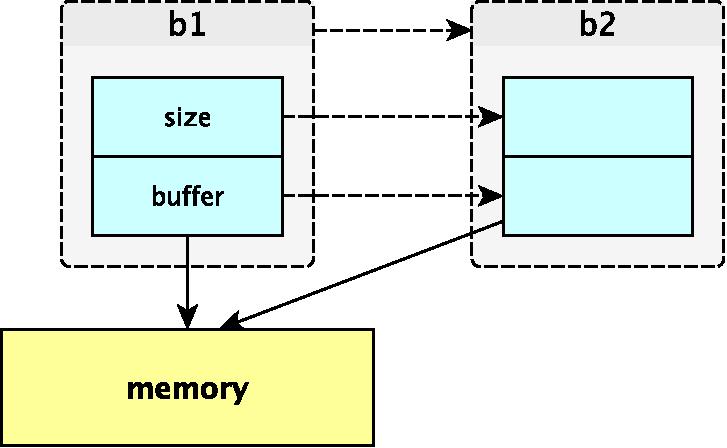
\includegraphics[width=0.6\textwidth]{illustrations/copying-crop.pdf}
\caption{Ошибка двойного освобождения}
\label{fig:copying-crop}
\end{figure}

Говорят, что по умолчанию C++ реализует поверхностное копирование (shallow copy\index{shallow copy}). Копирование с выделением нового буфера и копированием в него содержимого старого это глубокое копирование (deep copy\index{deep copy}) которое пользователь всегда должен реализовать самостоятельно. Ниже показано переопределение копирующего конструктора, о переопределении операторов и в частности оператора присваивания см. (\ref{OperatorOverloading})

\begin{lstlisting}
class CCopyableBuffer {
public:
  CCopyableBuffer(int size) : 
    m_size (size) m_buffer (new char[size]) {
  }
  ~CCopyableBuffer() { 
    delete[] m_buffer; 
  }
  CCopyableBuffer(const CCopyableBuffer& rhs) { 
    m_size = rhs.m_size; 
    m_buffer = new char[m_size];
    memcpy(m_buffer, rhs.m_buffer, m_size);
  } 
  char &get(int x) { 
     assert(x >= 0 && x < m_size); 
     return m_buffer[x]; 
  } 
private:
  char *m_buffer;
  int m_size;
};
\end{lstlisting}

Так всё будет работать. Но иногда копирование не нужно и его проще запретить, объявив собственные конструктор копирования и оператор присваивания в закрытой части класса.

\begin{lstlisting}
class NCBuffer {
public:
  NCBuffer(int size) : 
    m_size (size) m_buffer (new char[size]) {
  }
  ~NCBuffer() { 
    delete[] m_buffer; 
  }
  char &get(int x) { 
    assert(x >= 0 && x < m_size); 
    return m_buffer[x]; 
  }
private:
  char *m_buffer;
  int m_size;
  NCBuffer(const NCBuffer& rhs);
  NCBuffer& operator= (const NCBuffer& rhs);
};
\end{lstlisting}

Теперь компилятор не сгенерирует за вас неправильные варианты и копирование просто не будет скомпилировано.

Начиная с 2011 года, существует более цивилизованный способ запретить любой генерируемый по умолчанию метод или явно сгенерировать его -- ключевые слова \lstinline!default! и \lstinline!delete!.

\begin{lstlisting}
class NCBuffer {
public:
// .....
  NCBuffer(const NCBuffer& rhs) = delete;
  NCBuffer& operator= (const NCBuffer& rhs) = delete;
// .....
};
\end{lstlisting}

Человечное определение класса наподобие \lstinline!Empty!, которое не требует от программиста волшебных очков.

\begin{lstlisting}
struct Empty {
  Empty() = default;
  ~Empty() = default;
  Empty(const Empty &rhs) = delete;
  Empty& operator=(const Empty &rhs) = delete;
};
\end{lstlisting}

\textbf{Домашняя наработка:} поясните или опровергните мысль: ``именно из-за проблемы двойного освобождения, в C++ нет и не может быть простого аналога realloc''

Конечно писать RAII-обертку на каждый ресурс это очень накладно (в англоязычной литературе любят использовать в таких случаях термин boilerplate code). Поэтому профессионалы пишут одну обертку на все типы ресурсов -- так называемые умные указатели, которые будут рассмотрены в (\ref{SmartPointers}).

\subsubsection{Оптимизации возвращаемого значения\index{RVO}}\label{RVO}

RVO или оптимизация возвращаемого значения, прописана в стандарт C++ (например 12.3.2.15 для C++98) и она гласит, если коротко, что компилятор имеет право не вызывать копирующие конструкторы если он может статически доказать, что объекты эквивалентны.

Пример:

\begin{lstlisting}
#include <cstdio>

using namespace std;

class foo {
public:
  foo () { printf ("foo::foo()\n"); }
  foo (const foo&) { printf ("foo::foo( const foo& )\n"); }
  ~foo () { printf ("foo::~foo()\n"); }
};

foo
bar()
{
  foo local_foo;
  return local_foo;
}

int
main()
{
  foo f = bar();
  return 0;
}
\end{lstlisting}

В случае если GCC компилирует этот код без RVO (опция \lstinline!-fno-elide-constructors!), вывод на экран выглядит как:

\begin{lstlisting}
foo::foo()
foo::foo( const foo& )
foo::~foo()
foo::foo( const foo& )
foo::~foo()
foo::~foo()
\end{lstlisting}

Последовательность очевидна: создаётся локальный \lstinline!local_foo!, создаётся его копия -- возвращаемое значение, уничтожается \lstinline!local_foo!, возвращаемое значение копируется в \lstinline!f!, уничтожается возвращаемое значение, уничтожается \lstinline!f!.

В случае же обычной компиляции с RVO, вывод выглядит гораздо проще:

\begin{lstlisting}
foo::foo()
foo::~foo()
\end{lstlisting}

Эта экономия разрешена стандартом и поэтому программист не должен закладываться на то, что его конструктор копирования всегда будет вызван в контексте копирования.

\pagebreak
\subsection{Перегрузка\index{overload} операторов\index{operator}}\label{OperatorOverloading}

\hfill\textit{I left out operator overloading}

\hfill\textit{because I had seen too many people abuse it in C++}{\vspace{0.5em}}

\hfill\textit{-- James Gosling}

Язык C++ позволяет переопределять для пользовательских типов почти все операторы, которые применимы для встроенных типов, включая арифметические, логические, а также некоторые специального вида операторы. В прошлом разделе уже встречалось упоминание переопределения присваивания. Рассмотрим класс, абстрагирующий матрицу $N*M$ для $N>1, M>1$.

\textbf{Вопрос к студентам:} написать у доски то, что они уже знают: конструктор, деструктор, копирование, геттер/сеттер

\ifanswers
Возможный ответ:

\begin{lstlisting}
class Matrix
{
public:
  Matrix (int n, int m) : m_n (n), m_m (m), m_buf (new int[n*m]()) {}
  ~Matrix () { delete [] m_buf; }

  Matrix (const Matrix &rhs) : m_n (rhs.m_n), m_m (rhs.m_m), m_buf (new int[m_n * m_m])
    {
      std::memcpy (m_buf, rhs.m_buf, rhs.m_n * rhs.m_m * sizeof (int));
    }

  void set (int x, int y, int val) { m_buf[x*m_m + y] = val; }
  int get (int x, int y) { return m_buf[x*m_m + y]; }

private:
  int m_n, m_m;
  int *m_buf;
};
\end{lstlisting}
\fi

Допустим, хотелось бы написать сложение матриц.

\begin{lstlisting}
/* adds rhs to this and returns new sum matrix */
Matrix
Matrix::add (const Matrix &rhs)
\end{lstlisting}

Использование очевидно.

\begin{lstlisting}
Matrix m, n, t;
...
t.assign (m.add (n));
\end{lstlisting}

Но это не так красиво, как если бы допускалась более математическая запись с инфиксным сложением.

\begin{lstlisting}
t = m + n;
\end{lstlisting}

И C++, как вскоре станет ясно, даёт возможность переопределить операторы, такие как \lstinline!+!, \lstinline!=! и многие другие, чтобы добиться такой непосредственности в выражении мыслей.

Главная проблема здесь в том, что вы действительно вольны написать любой код в определении оператора сложения. Ваше сложение не обязано удовлетворять даже каким-то базовым инвариантам сложения:

\begin{lstlisting}
assert (a + b == b + a); /* ORLY? */
\end{lstlisting}

Вместо этого ваша операция сложения может осуществлять вычитание, лезть в базу данных или форматировать диск. Почти всегда, когда вы читаете код на C++, вы обязаны иметь в виду, что не можете быть уверены что значит операция \lstinline!+! этим утром. Ночью кто-нибудь мог вкоммитить в неё чудовищные изменения – из лучших побуждений, разумеется.

Всё усугубляется тем, что общий список операторов, которые можно переопределить, крайне внушающ. Его всегда можно посмотреть в стандарте, но кроме основных арифметических и логических операций, определение которых довольно таки прямолинейно, перегрузке могут подвергаться совершенно экзотические вещи – сравнение, присваивание, приведение к типу (любому, включая встроенные), обращение по указателю и даже выделение памяти с помощью new и её освобождение. Давайте побеседуем об нескольких специальных и проблематичных случаях переопределённых операторов.

\subsubsection{Операторы, формирующие цепочки}\label{ChainOps}

Первый особый случай, это операторы, которые могут быть записаны цепочками (обычно -- правоассоциативными). Скажем, пользователь оператора \lstinline!=!, скорее всего ожидает корректной работы строчки:

\begin{lstlisting}
x = y = z = w;
\end{lstlisting}

распространяющей, значение \lstinline!w! справа налево. Рассмотренный ранее (\ref{CopyConstr}) буфер может и должен быть расширен определение оператора равенства, который для того, чтобы такая цепочка могла быть сформирована, должен возвращать ссылку на текущий объект

\begin{lstlisting}
  CCopyableBuffer& operator= (const CCopyableBuffer& rhs)
  {
    if (&rhs == this) return *this;
    delete [] m_buffer;
    m_size = rhs.m_size; m_buffer = new char[m_size];
    memcpy(m_buffer, rhs.m_buffer, m_size);
    return *this;
  }
\end{lstlisting}

Особое внимание следует обратить на проверку \lstinline!if (&rhs == this)! в начале. Вторым способом написать эту проверку будет: \lstinline!if (rhs == *this)!

\textbf{Домашняя наработка:} почему второй способ может привести к некорректному и неожиданному поведению?

Большинство цепочечных операций: \lstinline!+=!, \lstinline!*=! и так далее, являются прямыми модификаторами состояния класса и должны быть определены в классе, чтобы у них был \lstinline!this! для возврата.

\subsubsection{Симметричные бинарные операторы}\label{SymmBinary}

Можно рассмотреть ещё один пример -- разработку класса, реализующего абстракцию комплексных чисел.

Для того, чтобы абстракция комплексных чисел была завершённой, должна быть возможность неявного преобразования double в complex, ведь по сути число \lstinline!2.0! это \lstinline!2.0 + 0.0 * i!. Эта возможность заложена в конструкторе класса (вспоминаем, что конструктор с одним аргументом это неявное преобразование типа).

\lstinputlisting[firstline=36,lastline=37]{cpp_code/p2s8.cpp}

Но здесь таится и опасность, потому что сложение перестаёт быть коммутативным и простая запись, вида:

\lstinputlisting[firstline=39,lastline=40]{cpp_code/p2s8.cpp}

Выдаст ошибку компиляции. Ошибка связана с тем, что неявные преобразования применяются только к параметрам, перечисленным в списке параметров. Поэтому \lstinline!a.operator+(2.0)! преобразует \lstinline!double! к \lstinline!Complex!, но для \lstinline!(2.0).operator+(a)! неявный параметр \lstinline!this! -- указатель на объект для которого вызывается метод, не подвергается, согласно стандарту, никаким неявным преобразованиям.

Правильный метод: определить операторы сложения и умножения вне класса как отдельные функции:

\lstinputlisting[firstline=8,lastline=29]{cpp_code/p2s8c.cpp}

Точно так же необходимо поступать со всеми функциями, которые по определению должны быть коммутативными. Тогда коммутативность будет сохранена.

Очень часто бинарные операции можно определить вне класса в терминах цепочечных операций, определенных в классе:

\begin{lstlisting}
Complex operator+ (Complex a, Complex b)
{
  Complex tmp = a;
  tmp += b;
  return tmp;
}
\end{lstlisting}

На самом деле, это предпочтительный метод. Он кроме всего прочего позволяет естественным образом сохранить когерентность \lstinline!+! и \lstinline!+=! или в общем случае -- цепочечной и соответствующей ей бинарной операции.

\subsubsection{Инкремент и декремент}\label{IncrOverload}

Язык C++ получил своё название от унарной операции \lstinline!x++!, которая увеличивает значение переменной в данном случае x, и возвращает старое значение. Такая операция называется постинкрементом. Известен также прединкремент \lstinline!++x!, который увеличивает свой аргумент и возвращает увеличенное значение.

\begin{lstlisting}
class Complex
{
public:
  Complex& operator++ ()
    {
      re += 1.0;
      return *this;      
    }
/*...*/
};
\end{lstlisting}

Такая запись возвращает прединкремент, он совсем простой. Постинкремент в терминах прединкремента может быть определен вот так:

\begin{lstlisting}
Complex operator++ (int unused)
{
  Complex result = *this;
  ++(*this);
  return result;
} 
\end{lstlisting}

Очевидно, что прединкремент в общем случае не требует копирования, которое, как уже выяснилось, может быть очень дорогим. Поэтому очень часто программисты на C++ используют именно прединкремент в циклах:

\begin{lstlisting}
for (Complex t = 1.0; t < 5.0; ++t) { ... }
\end{lstlisting}

вместо

\begin{lstlisting}
for (Complex t = 1.0; t < 5.0; t++) { ... }
\end{lstlisting}

Обычно замеры показывают что такая запись не несет какого-то особого выигрыша. Она просто показывает, что человек знает внутреннюю механику языка.

\subsubsection{Вызов и индексация}\label{BracketOverloading}

Эта перегрузка позволяет объекту быть вызванным как функция (с круглыми скобками и передачей аргументов).

\begin{lstlisting}
class LessThan
{
public:
  explicit LessThan(int x = 0) : m_x(x) {}
  bool operator()(int y) const { return y < m_x; }
private:
  int m_x;
}
\end{lstlisting}

Определённый таким образом класс, позволяет иметь сразу несколько функцие-подобных объектов (также они называются \textbf{функторы}\index{Functor}), выражающих предикаты ``меньше x'' для разных \lstinline!x!.

\begin{lstlisting}
LessThan ltthree(3), ltfour(4), ltfive(5);

assert(ltthree(2));
assert(!ltthree(4));
\end{lstlisting}

И вызывать их по необходимости.

Аналогично возможно перегрузить операцию взятия индекса.

\begin{lstlisting}
struct TwoArray {
  int y, int z;
  int& operator[] (int x) {
    if (x == 0) return y;
    if (x == 1) return z;
    // error processing
  }
}
\end{lstlisting}

При использовании такого класса, синтаксис мало чем отличается от массивов

\begin{lstlisting}
TwoArray t;
t[0] = 1;
t[1] = 2;
assert (3 == t[0] + t[1]);
\end{lstlisting}

Если не знать, невозможно догадаться, что реально никакого массива никто не выделяет.

\subsubsection{Разыменование и его варианты}\label{DereferenceOverloading}

Если есть классы, которые ведут себя как функции и массивы, логично предположить, что возможны классы, которые ведут себя как указатели. Для примера, можно рассмотреть так называемые умные указатели, о которых речь пойдет чуть дальше (см. \ref{SmartPointers}). Пусть есть несложная структура

\begin{lstlisting}
struct T {
  int x = 5;
  int foo (void) { return x; }
};
\end{lstlisting}

Можно изготовить класс, который будет вести себя почти как указатель на эту структуру

\begin{lstlisting}
class Tptr {
  T *t_;
public:
  Tptr(T *rhs) : t_(rhs) {};
  T operator*() const { return *t_; }
  T* operator->() const { return t_; }
};
\end{lstlisting}

В этом классе перегружены операторы обычного разыменования и разыменования с доступом к полю (часто для краткости его называют ``стрелкой''). Использование несложно.

\begin{lstlisting}
T t;
Tptr pt(&t);
pt->x = 6;
(*pt).foo();
\end{lstlisting}

Одной из важных особенностей перегрузки оператора стрелки является drill-down behaviour \index{Drill-Down behaviour} -- зарывающееся поведение: результат стрелки используется для разрешения имени, но если этого имени нет, то вместо него снова может быть выбран вызов стрелки.

\begin{lstlisting}
struct client { int a; };

struct proxy {
  client *target;
  client *operator->() const { return target; }
};

struct proxy2 {
  proxy *target;
  proxy &operator->() const { return * target; }
};

void f() {
  client x = { 42 };
  proxy y = { & x };
  proxy2 z = { & y };

  // prints 42 42 42
  printf ("%d %d %d\n", x.a, y->a, z->a);    
}
\end{lstlisting}

\textbf{Домашняя наработка:} в самой структуре \lstinline!T! теперь можно перегрузить \lstinline!operator&! который мог бы возвращать \lstinline!Tptr!, и таким образом, переписать код использования ещё проще. Попробуйте заставить это заработать.

В любом языке есть элементы бессмысленной джигитовки. В частности в C++ есть вызов по указателю на функцию:

\begin{lstlisting}
struct foo {
  int bar() { printf ("bar\n"); }
};

template <typename T>
void Apply (T* t, int (T::*bar)() ) {
  (t ->* bar) ();
}

int main (void) {
  int (foo::*pbar)() = &foo::bar;
  foo f;

  Apply (&f, pbar);

  return 0;
}
\end{lstlisting}

Скобки необходимы в \lstinline!Apply! поскольку приоритет \lstinline!->*! меньше, чем приоритет вызова функции.

Этот оператор тоже можно перегрузить. В перегрузке он самый неинтересный из всех операторов разыменования и ведет себя просто как произвольная бинарная операция. На самом деле он даже не обязан быть нестатическим!

Но помните: если вы обнаруживаете, что вы перегрузили \textbf{это}, значит у вас точно что-то пошло не так.

\subsubsection{Приведение типов}\label{CastOverloading}

Самый простой и в то же время самый богатый набор операторов это операторы приведения типов.

Пока что тут просто механическая копия с cppreference, TODO: расписать.

\begin{lstlisting}
struct X {
    //implicit conversion
    operator int() const { return 7; }
 
    // explicit conversion
    explicit operator int*() const { return nullptr; }
 
//   Error: array operator not allowed in conversion-type-id
//   operator int(*)[3]() const { return nullptr; }
    using arr_t = int[3];
    operator arr_t*() const { return nullptr; } // OK if done through typedef
//  operator arr_t () const; // Error: conversion to array not allowed in any case
};
 
int main()
{
    X x;
 
    int n = static_cast<int>(x);   // OK: sets n to 7
    int m = x;                     // OK: sets m to 7
 
    int* p = static_cast<int*>(x);  // OK: sets p to null
//  int* q = x; // Error: no implicit conversion
 
    int (*pa)[3] = x;  // OK
}
\end{lstlisting}

\begin{lstlisting}
struct To {
    To() = default;
    To(const struct From&) {} // converting constructor
};
 
struct From {
    operator To() const {return To();} // conversion function
};
 
int main()
{
    From f;
    To t1(f); // direct-initialization: calls the constructor
// (note, if converting constructor is not available, implicit copy constructor
//  will be selected, and conversion function will be called to prepare its argument)
    To t2 = f; // copy-initialization: ambiguous
// (note, if conversion function is from a non-const type, e.g.
//  From::operator To();, it will be selected instead of the ctor in this case)
    To t3 = static_cast<To>(f); // direct-initialization: calls the constructor
    const To& r = f; // reference-initialization: ambiguous
}
\end{lstlisting}


\pagebreak
\subsection{Выделение и освобождение динамической памяти}\label{MemManage}

Переопределение \lstinline!new! и \lstinline!delete! это всегда отдельная и крайне неприятная тема. Она связана с несколькими неочевидными ограничениями и десятком подводных камней. В общем случае, если вам понадобилось переопределять \lstinline!new! и \lstinline!delete!, подумайте ещё раз, может быть вы что-то сделали не так.

\subsubsection{Отличия new и malloc}\label{NewMalloc}

Есть два отличия \lstinline!new! от \lstinline!malloc! -- первое функциональное и второе идеологическое. 

С идеологической точки зрения, есть только одна пара глобaльных функций \lstinline!std::malloc! и \lstinline!std::free!, но при этом кроме соответствующей ей пары глобальных \lstinline!new! и \lstinline!delete!, существует также возможность переопределить выделение и освобождение памяти для каждого пользовательского типа.

С функциональной точки зрения можно говорить только об отличиях глобальных функций \lstinline!::operator new! и \lstinline!::operator delete! от глобальных функций \lstinline!std::malloc! и \lstinline!std::free!

Итак, \lstinline!std::malloc! и \lstinline!std::free! отличаются тем, что:

\begin{enumerate}
\item
Память аллоцируется из кучи (``Heap'')
\item
Возвращаемое значение имеет тип \lstinline!void*!
\item
При неудаче \lstinline!malloc! возвращает \lstinline!NULL!
\item
Требуют спецификации точного размера в байтах
\item
Выделение массива требует ручного подсчёта места на массив
\item
Перевыделение памяти просто (нет вызова копирующих конструкторов)
\item
Никогда не вызовут из себя \lstinline!new! или \lstinline!delete!
\item
Нет способа автоматически побить запрашиваемую память на более мелкие участки при нехватке памяти на большой линейный кусок
\item
Не могут быть легально переопределены ни в каком случае
\end{enumerate}

В отличие от них, \lstinline!::operator new! и \lstinline!::operator delete! имеют следующие свойства:

\begin{enumerate}
\item
Память аллоцируется из свободного хранилища (``Free Store''). Совпадает ли оно с кучей (``Heap'') упомянутой выше или это два разных места -- Implementation defined. Обычно в Unix совпадает, так как используется системный вызов sbrk, но есть варианты.
\item
Возращаемое значение -- типизированный указатель
\item
Обычно выбрасывает исключения при неудаче (см. ниже про специальные формы)
\item
Размер памяти вычисляется компилятором исходя из данного типа
\item
Есть версия специально для массивов
\item
Перевыделение памяти сложно (из-за вызова конструкторов) и нет его стандартной поддержки (аналога realloc)
\item
Вызовет ли из себя \lstinline!malloc! и \lstinline!free! зависит от реализации
\item
Поддерживает установку аллокатора для случая исчерпания памяти через \lstinline!set_new_handler!
\item
Могут быть легально переопределены для пользовательских типов
\item
Использует конструкторы для инициализации объектов и деструкторы для освобождения их ресурсов
\end{enumerate}

Наверное нет смысла заучивать эти отличия наизусть, но вместе они составляют консистентную картину, которую нужно понимать.

\subsubsection{Стандартные и специальные формы new}\label{PlacementNew}

Рассмотрим типичное выделение памяти в программе на C++:

\begin{lstlisting}
class Widget {};
...
Widget *w = new Widget;
\end{lstlisting}

Предположим, оператор \lstinline!new! не переопределён для класса \lstinline!Widget!

Что здесь происходит? Неожиданно много всего.

\begin{enumerate}
\item
Сначала, по форме оператора new, компилятор определяет какой именно new имеется в виду. Существуют три нормальные формы new:
\begin{itemize}
\item
\lstinline!new! в куче с возбуждением исключений при исчерпании памяти. Именно он использован в рассматриваемом примере.
\item
\lstinline!new! в куче с возвратом нуля при исчерпании памяти
\item
placement new (размещающий \lstinline!new!)\index{placement new} (с размещением в заданном месте). Именно он и был использован в листинге выше. Его синтаксис похож на выделяющий new из этого примера, но буфер, в котором размещается сконструированный объект, не выделяется, а передаётся как параметр в скобках.
\end{itemize}

Кроме нормальных существуют ещё и специальные формы new, когда пользователь некоего типа переопределяет размещающий new этого типа передавая ему не область памяти, а нечто иное -- скажем область памяти и поток для записи лога и т.п. В следующем листинге показано использование разных форм new.

\begin{lstlisting}
class Widget {};
...
Widget *w = new Widget;
Widget *w = new (std::nothrow) Widget;
Widget *w = new (WidgetPool) Widget;
Widget *w = new (WidgetPool, WidgetLogStream) Widget;
\end{lstlisting}

Здесь первая строчка это выделение памяти с возбуждением исключения при ошибке выделения и вызов конструктора. Вторая строчка это выделение памяти без возбуждения исключения при ошибки выделения (тогда в \lstinline!w! просто запишется нулевой указатель). Третья строчка это просто вызов конструктора на уже выделенную память (при этом неудачи выделения быть, разумеется, уже не может). И четвёртая строчка иллюстрирует специальную пользовательскую форму оператора \lstinline!new! и не будет скомпилирована, без специальных объявлений внутри класса \lstinline!Widget!.

\item
Далее компилятор выделяет память в куче (строго при необходимости, размещающие и специальные формы пропускают этот пункт) и в случае нехватки памяти вызывает пользовательский обработчик, который можно поставить и на стандартное выделение с помощью \lstinline!set_new_handler!.
\item
Далее в случае если вызвана нормальная форма неразмещающего new, компилятор вызывает конструктор размещённого в куче объекта или все конструкторы, если был размещён массив.
\item
Разрушение происходит в обратном порядке.
\end{enumerate}

Обычный сценарий работы \lstinline!malloc()! для выделения буфера, вместе с размещающим new для явного вызова конструктора приведён ниже:

\lstinputlisting{cpp_code/p2s9.cpp}

Обратите внимание -- деструктор может быть вызван явно.

\subsubsection{Список нормальных форм}\label{NewOverloading}

Ниже приведен класс для которого объявлены переопределения всех нормальных форм \lstinline!new!/\lstinline!delete! как это сделано в \cite{effcpp3d}.

\begin{lstlisting}
class StandardNewDeleteForms {
public:
static void *operator new(std::size_t size);
static void operator delete(void * memory);
static void *operator new(std::size_t size, const std::nothrow_t &nt);
static void *operator new(std::size_t size, void *ptr);
};
\end{lstlisting}

\textbf{Домашняя наработка:} Напишите и протестируйте код для каждого из переопределений.

C++ предоставляет достаточно тонкий инструментарий для работы с памятью, который необходимо использовать с осторожностью. Переопределяя каждый оператор не забывайте о возможном пользовательском вызове \lstinline!set_new_handler!. Переопределяя \lstinline!new! не забывайте переопределять соответсвующий \lstinline!delete!. Работайте с памятью осторожно и внимательно. И главное -- трижды подумайте нужно ли вам это вообще.

\pagebreak
\subsection{Правые ссылки и семантика перемещения}

Ссылки (references) это то, что наиболее сложно воспринимается при переходе с C на C++. Человеку с опытом программирования на C, может быть непонятно, зачем они нужны, когда уже есть такие удобные и привычные указатели, которые позволяют делать всё то же самое только лучше... Подлинное осознание того, каким именно инструментом являются ссылки и как ими оперируют, приходит с опытом C++. При переходе на новый стандарт C++11, идея о том, что теперь есть ещё один вид ссылок -- ссылки на rvalue (rvalue references) кажется новаторской и неочевидной (особенно неочевидна её полезность). Скорее всего, многим придётся преодолеть внутреннее сопротивление, прежде чем rvalue references станут удобным и привычным инструментом. 

\subsubsection{Ещё раз про категории значений}\label{LRvaluesAgain}

Прежде, чем переходить к описанию rvalue references, есть смысл немного вспомнить о том, что такое rvalue и lvalue.

Термин lvalue был, прежде чем перейти в C++, документально зафиксирован в стандарте языка C, поэтому логично начать изложение с него. Для языка C, lvalue (от left hand side value) -- то, что может появиться слева в выражении присваивания. Формально (6.3.2.1 стандарта C99), ``An lvalue is an expression with an object type or an incomplete type other than void'' (под object type в стандарте понимаются все типы, не являющиеся function type или incomplete type).

\begin{lstlisting}
int c = a * b;
a * b = 42;
foo() = 42;
\end{lstlisting}

Собственно, в стандарте языка C90 и последовавшем за ним C99 нет термина rvalue. В C99 есть оговорка ``What is sometimes called ``rvalue'' is in this International Standard described as the ``value of an expression'''', позволяющая предположить, что к этому времени этот термин существовал и использовался, но фиксировать его строго в случае языка C было не нужно.

Всё изменилось с приходом языка C++, который принёс с собой ссылки (lvalue references). Выражение из прошлого примера:

\begin{lstlisting}
foo() = 42;
\end{lstlisting}

может быть ошибкой если foo возвращает значение, но совершенно корректно, если foo возвращает ссылку. Чтобы разрешить эту неоднозначность, стандарт C++ 98 объявляет (3.10.1) два термина -- lvalue и rvalue, причём каждое выражение языка C++98 является либо тем, либо другим. При этом определение в (3.10.2) гласило ``An lvalue refers to an object or function''.

То есть lvalue это не первоклассный объект как в C, а просто некое выражение ссылающееся на область памяти. Таким образом в качестве главного различия выступает возможность взять адрес, а не отношение к операции равенства.

\begin{lstlisting}
int& foo();
foo() = 42;
int* p1 = &foo();
int foobar();
int* p2 = &foobar();
\end{lstlisting}

Таким образом, lvalue в C++98 приобретает смысл locator value (а не left hand side value). Так, например если есть \lstinline!int *val!, то выражение \lstinline!val+1! можно разыменовать, но нельзя взять его адрес.

\begin{lstlisting}
int *val;
int correct = *(val + 1);
int **wrong = &(val + 1);
\end{lstlisting}

При этом в качестве двух облаков на горизонте языка маячили проблемы семантики перемещения и совершенного форвардинга.

Семантика перемещения может быть проиллюстрирована проблемой COAP (см. \ref{COAP}) -- действительно контейнеры из \lstinline!auto_ptr! вели себя странно, потому что перемещение и копирование никак не были разделены: в языке была возможность написать \lstinline!a = b! но не \lstinline!move(a,b)! и заложенная в переопределенный оператор присваивания семантика перемещения оказалась миной: рано или поздно так или иначе кто-то все равно использует присваивание как присваивание.

Совершенный форвардинг это та же проблема в приложении к формальным аргументам функций, речь о ней пойдет чуть ниже.

Как ни странно, но чтобы решить эти две простые проблемы, потребовалось очень глубокое пересомысление терминологии и существенная доработка стандарта.

Cтандарт C++11 объявляет (3.10) пять терминов, которые проиллюстрированы на диаграмме (рис. \ref{fig:val_category}). Содержательно произошло следующее: некогда единые rvalues были разбиты на два класса: значения с истекающим сроком годности (xvalues), и чистые rvalues такие как арифметические константы или результаты арифметических операций. В то же время, lvalues и xvalues были обобщены в glvalues по причинам, которые получат своё объяснение позже.

\begin{figure}[ht]
\centering
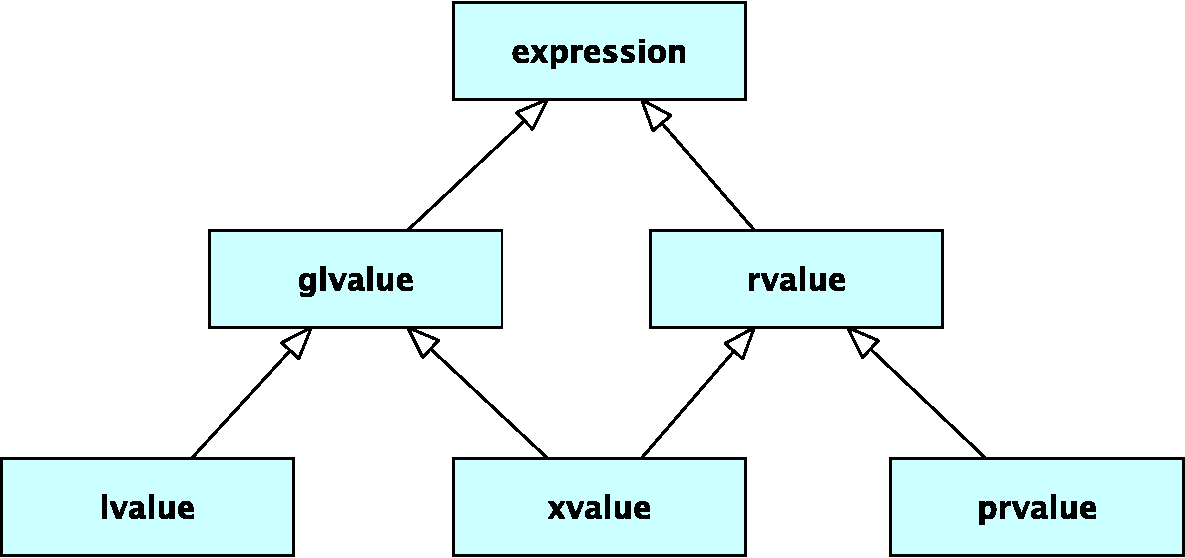
\includegraphics[width=1.0\textwidth]{illustrations/value-cat-crop.pdf}
\caption{Виды значений в C++11}
\label{fig:val_category}
\end{figure}

Более точно в новом стандарте регламентировано, что:

\begin{itemize}
\item \textbf{lvalue} -- выражение, идентифицирующее постоянный объект или свободную функцию. Должны быть доступны: взятие адреса, использование в левой части выражения (при неконстантности) и инициализация таким выражением левой ссылки:
\begin{lstlisting}
int lval;
int *t = &++lval;
lval = 2;
int &lref = lval;
\end{lstlisting}
Ещё говорят, что у lvalues есть identity (прописка) -- то есть каждый такой объект можно как-то отличить от любого другого (взять адрес, etc)
Если тип выражения expr это lvalue \lstinline!T!, то \lstinline!decltype(expr)! это \lstinline!T&!
\item \textbf{xvalue} -- выражение, идентифицирующее объект с истекающим временем жизни. Это очень странные объекты, которые были введены именно для поддержки rvalue ссылок. Большая часть исследуемых в этом разделе объектов будет xvalue.
Если тип выражения expr это xvalue \lstinline!T!, то \lstinline!decltype(expr)! это \lstinline!T&&!
\item \textbf{prvalue} -- выражение, идентифицирующее временный объект или значение не ассоциированное ни с каким объектом. В частности это литералы, вызовы функций которые возвращают не ссылку, и все остальное, что раньше называлось rvalue
Если тип выражения expr это prvalue \lstinline!T!, то \lstinline!decltype(expr)! это \lstinline!T!
\item \textbf{glvalue} -- то, что раньше называлось lvalue -- обобщение lvalue и xvalue. При этом glvalue может быть полиморфным объектом, его динамический тип не обязан совпадать со статическим.
\item \textbf{rvalue} -- отрицание lvalue. Это не адресуемый, не используемый в левой части объект. Им можно инициализировать константные левые ссылки
\end{itemize}

Первые три категории являются базовыми. Чуть ниже будет предъявлен способ различить к какой категории относится объект на этапе выполнения, но чтобы это сделать, сначала необходимо поговорить о том, чем же все таки являются правые ссылки.

\subsubsection{Отличия правых и левых ссылок}\label{RvalueRefs}

В C++11, если X это тип, то \lstinline!X&! это lvalue reference, а \lstinline!X&&! это rvalue reference для этого типа (8.3.2.2). При этом важно понимать -- \lstinline!X&, X&&! -- это разные типы, но семантически они эквивалентны и о них можно вместе говорить как о ``ссылках вообще''. Тем не менее, поскольку это разные типы, для них работает перегрузка:

\begin{lstlisting}
int a, b;
foo(int &x);
foo(int &&x);
foo(a * b); /* calls foo (int &&x) */
foo(a);     /* calls foo (int &x) */
\end{lstlisting}

При этом сама по себе rvalue reference может быть lvalue (и является им, если она именована).

\begin{lstlisting}
int a = 3, b = 5;
int &&x = a * b;
int &y = x; // works!
x = x + 1; // works!
y = y + 1; 
foo(x); /* calls foo (int &x) !!! */
cout << x << endl;
\end{lstlisting}

На экране будет 17.

Это очень важное правило. Легко представить ситуацию, в которой объявлен класс Base и в нём есть необходимость определить конструкторы:

\begin{lstlisting}
Base(Base const & rhs);
Base(Base&& rhs);
\end{lstlisting}

Теперь в наследуемом от него классе Derived, есть необходимость эти конструкторы переопределить. С первого взгляда можно сделать это следующим образом:

\begin{lstlisting}
Derived(Derived const & rhs) : Base(rhs) {};
Derived(Derived&& rhs) : Base(rhs) {};
\end{lstlisting}

Перемещающий конструктор переопределён неверно -- поскольку rhs имеет имя, оно есть lvalue, а значит \lstinline!Base(rhs)! в данном случае вызовет снова \lstinline!Base(Base const & rhs)!, что, вероятно, не желательно. Вместо этого следует писать

\begin{lstlisting}
Derived(Derived&& rhs) : Base(std::move(rhs)) {};
\end{lstlisting}

Говорят, что \lstinline!std::move! скрывает имя \lstinline!rhs!, делая его таким же безымянным rvalue выражением, как \lstinline!a*b!. Это общее правило ``оно не должно иметь имени'' очень полезно для выработки интуиции.

Addendum: упомянутый \lstinline!std::move! позволяет взять правую ссылку на что угодно (возможно испортив это ``что угодно''). Также можно взять указатель от любой переменной обладающей адресом. Но можно ли получить анонимную ссылку на переменную в том же смысле, в каком можно получить анонимный указатель на неё взятием адреса? Да, можно и для этого служит \lstinline!std::ref!. На самом деле он возвращает не ссылку а ссылко-подобный объект \lstinline!std::reference_wrapper!. Пока может быть непонятно зачем он может быть нужен, но его следует запомнить так как к нему предстоит вернуться (см. \ref{Binding}).

\subsubsection{Висячие ссылки и связывание ссылок}\label{DanglingRRefs}\index{Dangling references}

Проблема висячих ссылок (dangling references) известна давно и каждому программисту. Для левых ссылок она была рассмотрена ранее в (\ref{DanglingRefs})

\begin{lstlisting}
void simple_dangle ()
{
  int *myArray;
  myArray = new int[2]{ 100, 200 };
  int& ref = myArray[0];
  delete[] myArray;
  cout << "100 = " << ref << endl;  // dangling reference  
}
\end{lstlisting}

Такие проблемы может отследить даже valgrind. Аналогично ссылка может повиснуть если возвращать из функции ссылку на временный объект. Последний GCC выдает на эту тему warning.

\begin{lstlisting}
int& __attribute__ ((noinline))
refret (int x)
{
  return x;
}
\end{lstlisting}

При простейшем использовании:

\begin{lstlisting}
int &v = refret (3);
cout << v << endl; /* ! */
\end{lstlisting}

Вы подписываетесь на приключения. На удивление, следующий код безопасен:

\begin{lstlisting}
int xret (int x)
{
  return x;
}

const int &lv = xret (1);
int &&rv = xret (1);
cout << lv << " " << rv << endl;
\end{lstlisting}

Всё будет хорошо. Здесь const reference binding продляет время жизни временного объекта. Обратите внимание: ссылка связана с временным объектом. При попытке использовать там неконстантную ссылку ничего работать не будет. Но можно (как и показано выше) продлить объект правой ссылкой. Поскольку объект, возвращаемый функцией в данном случае является prvalue, здесь не будет никаких проблем. Между прочим, так можно связывать ссылку с любым prvalue, даже с константой:

\begin{lstlisting}
const int &lv = 0; // ok
int &&rv = 0; // ok
\end{lstlisting}

Будет создан временный объект со сроком жизни равным сроку жизни ссылки. Это порождает один хитрый вопрос:

\begin{lstlisting}
struct Base {};
struct Derived : public Base {};

Derived __attribute__ ((noinline))
derivedret ()
{
  return Derived ();
}

void
tricky_1 ()
{
  const Base &corr = derivedret ();
  /* use corr */
} /* which destructor? */
\end{lstlisting}

Какой деструктор будет вызван в этом случае? Оказывается статический тип временного объекта известен компилятору и будет вызван деструктор класса \lstinline!Derived!. То есть ссылки не требуют виртуальных деструкторов для своей диспетчеризации -- компилятор сам может построить верный код удаления.

Пока что все выглядит хорошо. Давайте проверим:

\textbf{Вопрос студентам:} что будет выведено на экран следующим кодом:

\begin{lstlisting}
int &
lr_ret (int x)
{
  return std::ref(x);
}
/* .... */
int &x = lr_ret(3);
cout << x << endl;
\end{lstlisting}

\ifanswers
Правильный ответ: что угодно, это dangling reference.
\fi

\textbf{Вопрос студентам:} что будет выведено на экран следующим кодом:

\begin{lstlisting}
int &&
rr_ret (int x)
{
  return std::move(x);
}
/* .... */
int &&x = lr_ret(3);
cout << x << endl;
\end{lstlisting}

\ifanswers
Правильный ответ: и снова что угодно. Получилась удивительную вещь: \textbf{dangling rvalue reference}. Так же как висячих левых, надо опасаться висячих правых ссылок. Опять-таки есть способы их получить:

\begin{lstlisting}
extern int xret (int x);
int &&p = xret (3); /* ok */
int &&p = std::move (xret (3)); /* dangling rvalue reference */
\end{lstlisting}
\fi

\textbf{Вопрос к студентам:} были рассмотрены dangling lvalue и rvalue references. Можно ли организовать dangling const reference?

\ifanswers
Правильный ответ: тысячей способов. Из экзотики есть способ прострелить себе ногу с помощью \lstinline!initializer_list! когда он является аргументом \lstinline!new! (пример из 12.2.5 стандарта C++14): 

\begin{lstlisting}
struct S { int mi; const pair<int,int>& mp; };
S a { 1, {2,3} }; // ok
S* p = new S{ 1, {2,3} }; // Creates dangling const reference
\end{lstlisting}

Хотя вроде \lstinline!const pair&! продлевает время жизни, но new-initializer подчиняется особым правилам.
\fi

Понимание того как живут rvalue references и временные объекты, позволяет использовать класс, сочетающий левые и правые ссылки:

\begin{lstlisting}
struct RefBind
{
  int& ref;

  RefBind(int&& r) : ref(r) {}

  RefBind const& plus(int x) const { ref += x; return *this; }
  RefBind const& mult(int x) const { ref *= x; return *this; }

  int get() const { return ref; }
};
\end{lstlisting}

Три сценария использования:

\begin{lstlisting}
  int x = 1;

  std::cout << RefBind(1).plus(2).mult(3).get() << std::endl;
  std::cout << RefBind(std::move(x)).plus(2).mult(3).get() << std::endl;
  std::cout << RefBind(int(x)).plus(2).mult(3).get() << std::endl;
\end{lstlisting}

Первая строчка работает с чисто временным объектом, привязанным к lvalue ссылке и поэтому модифицируемым. Вторая попутно изменяет значение переменной \lstinline!x!, третья делает из переменной временный объект и работает с ним.

\textbf{Вопрос к студентам:} что будет если попытаться использовать значение объекта типа \lstinline!RefBind! после конца полного выражения?

\begin{lstlisting}
RefBind x(1);
std::cout << x << std::endl;
\end{lstlisting}

\ifanswers
Правильный ответ: dangling rvalue reference.
\fi

\subsubsection{Свёртка ссылочных типов}\label{ReferenceConvolution}

Ccылка на ссылку -- невозможна. Это все знают и тысячу раз отвечали на собеседованиях. Что же, этот ответ всё ещё верен и стандарт C++11 (8.3.2.5) запрещает ссылки на ссылки, указатели на ссылки и массивы ссылок. Но как быть, когда в шаблоне или при \lstinline!typedef! получается смесь правых и левых ссылочных типов? Это способно поставить в тупик.

Стандарт (8.3.2.6) определяет следующие правила свёртки ссылок, применимые для определений \lstinline!auto! и \lstinline!decltype!, \lstinline!typedef!, а также параметров шаблонов:

\lstinline!A& &! становится \lstinline!A&!
\lstinline!A& &&! становится \lstinline!A&!
\lstinline!A&& &! становится \lstinline!A&!
\lstinline!A&& &&! становится \lstinline!A&&!

Самый простой пример использует уже рассмотренное \lstinline!auto!, вывод типов шаблонами можно отложить до (\ref{TemplateInference}).

\begin{lstlisting}
int i = 42;
auto&& ri_1 = i;  /* int& ri_1 */
auto&& ri_2 = 42; /* int&& ri_2 */
\end{lstlisting}

Интересно, что здесь двойной амперсанд может означать и lvalue и rvalue ссылку. Стоит запомнить эту идею: скоро она получит свое развитие.

\subsubsection{Добавление и удаление ссылок}

Стандарт определяет функтор \lstinline!remove_reference! (20.9.7.2), который позволяет получить не-ссылочный тип из ссылочного. Он работает похоже на \lstinline!static_cast! и прочие привычные вещи. Аналогично (но наоборот) работает пара \lstinline!add_lvalue_reference!/\lstinline!add_rvalue_reference!. Этот функтор позволяет, например, безопасно написать минимум для смешанных типов:

\begin{lstlisting}
template <typename T, typename S>
auto min(T x, S y) -> 
  remove_reference <decltype(x < y ? x : y)>::type 
{
  return x < y ? x : y;
}
\end{lstlisting}

Что решает задачу, поставленную выше (см. \ref{DeclFunctions}).

Также это решает проблему продирания \lstinline!decltype! через конструкторы. Специальный функтор \lstinline!declval! возвращает \lstinline!add_rvalue_reference<T>::type!, что даёт возможность писать \lstinline!decltype! в сложных случаях:

\begin{lstlisting}
struct Default {
    int foo() const {return 1;}
};
 
struct NonDefault {
    NonDefault(const NonDefault&) {}
    int foo() const {return 1;}
};
 
decltype (Default().foo()) n1 = 1; // int n1
// decltype(NonDefault().foo()) n2 = n1; // will not compile
decltype (declval<NonDefault>().foo()) n2 = n1; // int n2
\end{lstlisting}

Можно рассматривать \lstinline!declval<S>()! как изящный способ написать \lstinline!*(S *)nullptr!

\begin{lstlisting}
decltype((*(NonDefault*)nullptr).foo()) n2 = n1; // int n2
\end{lstlisting}

Но есть случаи когда \lstinline!declval! круче и они тоже касаются ссылок:

\begin{lstlisting}
using S = int &;
using T = decltype(declval<S>()); // collapsed ok
using U = decltype(*(S *)nullptr); //boom!
\end{lstlisting}

Пара функторов \lstinline!is_lvalue_reference! и \lstinline!is_rvalue_reference! позволяют определять на этапе исполнения к какой базовой категории относится конкретный тип \lstinline!T! (для этого надо применить к нему \lstinline!std::remove_reference! и проверить получившийся тип). 

\begin{itemize}
\item lvalue если сработало условие \lstinline!is_lvalue_reference!
\item xvalue если сработало условие \lstinline!is_rvalue_reference!
\item prvalue, если не сработало ни одно из них
\end{itemize}

\textbf{Вопрос к студентам:} как определить glvalue и rvalue?

\ifanswers
Правильный ответ: glvalue это lvalue or xvalue и дальше побитовыми операциями
\fi

\subsubsection{Обмен выражениями и перемещение}

Удовлетворяющая стандарту реализация библиотечной функции \lstinline!std::swap! (C++11 20.2.2) может выглядеть, например, так:

\begin{lstlisting}
template <typename T> 
void swap(T& a, T& b) 
{ 
  T tmp(std::move(a)); // move-ctor T
  a = std::move(b);    // move-assignment T
  b = std::move(tmp);  // move-assignment T
} 
\end{lstlisting}

В этой реализации нет операций копирования (без которых не обойтись в C++98). Специальная реализация move-конструкторов позвоялет отличать их от copy-конструкторов и делает гораздо легче. Представьте, что \lstinline!T! это некий \lstinline!MemoryBlock!. Тогда возможный вид конструкторов:

\begin{lstlisting}
/* copy ctor */
MemoryBlock(const MemoryBlock& other)
   : m_length(other.m_length), m_data(new int[other.m_length])
{
  std::copy (other.m_data, other.m_data + m_length, m_data);
}

/* move ctor */
MemoryBlock(MemoryBlock&& other) 
   : m_data(other.m_data), m_length (other.m_length)
{
   other.m_data = NULL;
   other.m_length = 0;
}
\end{lstlisting}

Функция \lstinline!std::move! позволяет здесь реализовать семантику перемещения, поскольку она работает так: из любого аргумента, \lstinline!std::move! делает rvalue reference. Эта функция в свою очередь, в удовлетворящем стандарту (20.2.3) виде может быть определена так:

\begin{lstlisting}
template <typename T> 
typename remove_reference<T>::type&&
std::move(T&& a) noexcept
{
  typedef typename remove_reference<T>::type&& RvalRef;
  return static_cast<RvalRef>(a);
} 
\end{lstlisting}

Методологически полезно проследить, что будет если вызвать \lstinline!std::move! с аргументом, имеющим тип \lstinline!X! и являющимся lvalue.

1) T будет разрешено в \lstinline!X&!
2) тип аргумента \lstinline!X& &&! a будет свёрнут в \lstinline!X&! a
3) \lstinline!remove_reference<X&>::type&&! будет означать \lstinline!X&&!, который и будет значением \lstinline!RvalRef!

Итак, получим эквивалент:

\begin{lstlisting}
X&& std::move(X& a) noexcept
{  
  return static_cast<X&&>(a);
}
\end{lstlisting}

Что и требовалось.

\textbf{Вопрос к студентам:} Так почему бы не писать \lstinline!static_cast<X&&>(x)! вместо \lstinline!std::move!?

\ifanswers
Правильный ответ: заворачивание в шаблон в данном случае позволяет неявный вывод шаблонного параметра, что делает запись удобней. А так пожалуйста.
\fi

Сама идея, что теперь обмен значениями может быть семантически выражен как обмен значениями, а не копирование (а значит и соптимизирован соответствующим образом) после её осознания, приводит людей в лёгкую эйфорию. В конце концов стремление к максимальной эффективности -- нормальное стремление. Тем не менее, с функцией \lstinline!std::move! следует быть осторожным. Часто идея вернуть \lstinline!std::move(x)! вместо \lstinline!x!, когда реально нужно rvalue и хочется избежать лишних копирований, приводит к отключению оптимизаций возвращаемого значения (\ref{RVO}) в компиляторе и результат ухудшается. Большинство таких трансформаций на современных компиляторах требует замеров и не должны выполняться preliminary:

\begin{lstlisting}
X&& foo()
{
  X x;
  return std::move(x); // bad idea
}
\end{lstlisting}

Итак, rvalue references позволяют (совместно с \lstinline!std::move!) по новому взглянуть на ссылки и открывают простор к более тонкому различию таких терминов естественного языка как ``копирование'', ``присваивание значения'', ``присваивание результата'' на языке C++, что открывает как простор к оптимизациям, так и возможности более аккуратного выражения старых идиом (хороший пример блестящего использования правых ссылок это \lstinline!std::unique_ptr! который в новом стандарте пришёл на смену печально известному \lstinline!auto_ptr!). 

\begin{lstlisting}
  auto_ptr <int> told (new int(2));
  auto_ptr <int> sold (new int(3));

  told = sold;

  unique_ptr <int> t (new int(2));
  unique_ptr <int> s (new int(3));

  // t = s; -- compilation error, no copy ctor
  t = std::move (s); // -- ok, move ctor
\end{lstlisting}

Но настоящую силу в контексте обобщенного программирования правые ссылки приобретают благодаря своим универсальным свойствам.

\subsubsection{Universal references}\index{Universal references}\label{UniversalReferences}

Как уже было показано выше, благодаря свертке ссылочных типов (\ref{ReferenceConvolution}) двойные амперсанды в объявлении типов и аргументах шаблонов имеют два разных значения:

\begin{lstlisting}
  /* rvalue references */
  Widget&& var1 = someWidget; 
  template<typename T> void f(std::vector<T>&& param);
     
  /* NOT rvalue references */
  auto&& var2 = var1; 
  template<typename T> void g(T&& param);
\end{lstlisting}

В первых двух случаях \lstinline!var1! и параметр функции \lstinline!f! это честные rvalue references. Во вторых двух случаях они зависят от вывода (в том числе -- свертки) типов.

\begin{lstlisting}
  int t;
  auto&& var2 = t; /* decltype (var2) == int& */
\end{lstlisting}

В этом контексте \lstinline!var2! это левая а не правая ссылка по правилам свертки типов. Поскольку \lstinline!var2! может разрешиться в любую ссылку -- как в левую, так и в правую, она называется \textbf{универсальной} ссылкой. Здесь и далее при разговоре про универсальные ссылки будем считать что сам тип \lstinline!T! ссылкой не является -- иначе к и без того сложному разговору добавиться необходимость учета ссылочного свертывания.

Важно понимать, что универсальность ссылки сохраняется только в контекстах чистого автоматического вывода. Даже следующий простой пример:

\begin{lstlisting}
template<typename T> void f(const T&& param);
\end{lstlisting}

Означает обязательно правую, ни в коем случае не универсальную ссылку. 

Здесь также видна существенная разница между \lstinline!auto! и \lstinline!decltype!, поскольку механизм \lstinline!decltype! зависит только от вывода типа внутри выражения:

\begin{lstlisting}
Widget w1, w2;
auto&& v1 = w1; /* Ok, v1 is Widget& */
decltype(w1)&& v2 = w2; /* Error! */
decltype(w1)&& v2 = std::move(w2); /* Ok, v2 is Widget&& */
\end{lstlisting}

Таким образом, универсальные ссылки в контексте \lstinline!decltype! невозможны.

\textbf{Вопрос к студентам:}

\begin{lstlisting}
template <typename T> void f(T &a);  /* (1) */
template <typename T> void f(T &&a); /* (2) */

int a;
f(a); /* ? */
f(1); /* ? */
\end{lstlisting}

\ifanswers
Знание об универсальных ссылках теперь должно подсказать правильный ответ: оба раза будет вызвана вторая функция. Это надо запомнить как правило (прописано в новой книжке Майерса \cite{effmoderncpp}): никогда не перегружайте функции по универсальной ссылке.
\fi

На самом деле с перегрузкой все даже более сложно. Дело в том, что универсальные ссылки ведут себя в перегрузке очень ``жадно''.

\begin{lstlisting}
template <typename T> void f(const T &a);  /* (1) */
template <typename T> void f(T &&a); /* (2) */
void f(int x); /* (3) */

f(10); // (3)
f('s'); // (2)!
f(10u); // (2)!
\end{lstlisting}

Несмотря на то, что в третьем случае у нас есть преобразование, будет выбрана универсальная ссылка. Это не похоже ни на что, даже на то, что шаблоны вообще-то делают по умолчанию (см. \ref{TemplOverloading}, корень проблемы станет ясен там же)

\subsubsection{Проброс типов}\label{PerfectForw}\index{Perfect Forwarding}

Простая оболочка над фабрикой классов, которая в идеале должна просто прокидывать свой аргумент с минимальными изменениями в конструктор, создает очевидную проблему лишнего копирования для своего формального параметра:

\begin{lstlisting}
template<typename T, typename Arg> 
T* factory(Arg arg)
{ 
  T *retval = new T(arg)
  return retval;
} 
\end{lstlisting}

Попытка её решить, заменив передачу по значению на передачу по ссылке натыкается на очевидное возражение -- может быть важный сценарий использования с передачей туда, например, констант. Или результатов функций, созвращающих значение, etc.

Прошаренный человек может предложить в этом случае добавить перегрузку по константной ссылке. 

\begin{lstlisting}
T* factory(Arg &arg);
T* factory(const Arg &arg);
\end{lstlisting}

Хорошо. Но представим у нас несколько аргументов. 

\begin{lstlisting}
T* factory(Arg arg1, Arg arg2, Arg arg3, Arg arg4);
\end{lstlisting}

Тогда учет сочетания всех константных и неконстантных ссылок довольно быстро приводит к комбинаторному взрыву (16 перегрузок это чуть больше, чем хотелось бы).

Решение проблемы выглядит несколько необычно:

\begin{lstlisting}
template<typename T, typename Arg> 
shared_ptr<T> factory(Arg&& arg)
{ 
  return shared_ptr<T>(new T(std::forward<Arg>(arg)));
} 
\end{lstlisting}

Здесь \lstinline!std::forward! это довольно прозрачная оболочка, в чем-то похожая на \lstinline!std::move!

\begin{lstlisting}
template<class S> S&& 
forward(typename remove_reference<S>::type& a)
{
  return static_cast<S&&>(a);
} 
\end{lstlisting}

Идея этого функтора в том, что используя механизм универсальных ссылок он приводит свой аргумент к lvalue-ссылке если сам этот аргумент lvalue и к rvalue-ссылке в противном случае. Это и есть perfect forwarding -- совершенная передача аргументов, которой всем так не хватало в старом добром C++.

\textbf{Вопрос к студентам:} А зачем вообще нужен \lstinline!remove_reference<S>::type&!? Кажется, простое использование \lstinline!S&! свернет ссылки точно так же.

\ifanswers
Ответ: это исключает неявный вывод параметра для шаблона.
\fi

\subsubsection{Проброс ссылок}\label{PerfectForwRef}

Важной проблемой относительно правых ссылок является проброс правой ссылки (с присущей ей move-семантикой) через цепочку функций. Наивная попытка такого проброса может выглядеть как-то так:

\begin{lstlisting}
void g(int &&t); /* 1 */
void g(int &t);  /* 2 */

void h(int &&t) { g(t); } /* always 2 */

h(1);
\end{lstlisting}

Увы, это не работает. Даже менее наивная попытка с использованием универсальных ссылок (\ref{UniversalReferences}) проваливается:

\begin{lstlisting}
template <typename T>
void h2(T &&t) { g(t); } /* always 2 */
\end{lstlisting}

Конечно можно выйти из положения с явным \lstinline!std::move! следующим образом:

\begin{lstlisting}
template <typename T>
void h3(T &&t) { g(std::move(t)); } /* always 1 */
\end{lstlisting}

Но увы, это решение шатает в другую крайность -- теперь даже вызовы с lvalue будут идти по rvalue маршруту. Решение проблемы является использование \lstinline!std::forward<T>!

\begin{lstlisting}
template <typename T>
void h4(T &&t) { g(std::forward<T>(t)); }
\end{lstlisting}

Теперь наконец-то можно различить что и по какой ветке было вызвано

\begin{lstlisting}
int x = 0;
h4(1); /* calls 1 */
h4(x); /* calls 2 */
\end{lstlisting}

Название это техники perfect forwarding способно сбивать с толку. Он не столь уж и perfect в том смысле, что, например, не способен решить проблему перегрузки универсальной ссылки.

Хорошей иллюстрацией техники совершенной проброски аргументов будет обещанная ранее совершенно прозрачная оболочка над функцией. Увы, она требует variadic templates, так что придется ещё немного потерпеть (см. \ref{PerfectCloth}).

\textbf{Домашняя наработка:} как все-таки решить проблему перегрузки универсальной ссылки из раздела (\ref{UniversalReferences})?

\subsubsection{Reference qualifiers}

Малоизвестной особенностью современного C++, упоминаемой например в \cite{effmoderncpp}, является наличие у методов классов reference qualifiers. Они похожи на const из (\ref{Selectors}), но не являются частью интерфейса функции, а наоборот позволяют версионировать её вызов для разных объектов:

\begin{lstlisting}
struct Widget {
  Data& get_data() &;
  Data get_data() &&;
};
\end{lstlisting}

Здесь первая функция будет вызвана только в том случае, если объект класса \lstinline!Widget! является lvalue, а вторая если он является rvalue. Перегрузка функции также по типу позволяет в первом случае вернуть ссылку, а во втором случае сконструировать необходимый объект.

\pagebreak
\subsection{Наследование интерфейса\index{Inheritance}\index{Interface inheritance}}\label{IntfInheritance}

\hfill\textit{If you think C++ is not overly complicated, just what is} 

\hfill\textit{a protected abstract virtual base pure virtual private destructor?}

\hfill\textit{And when was the last time you needed one?}{\vspace{0.5em}}

\hfill\textit{-- Tom Cargill}

Программа, в которой важной абстракцией является физический объект, иногда подразумевает сложные архитектурные решения, относительно представления этого объекта. Координаты нужны (почти) всем физическим объектам, но как быть с массой, с радиусом, с электрическим зарядом, с любыми дополнительными параметрами? Конечно можно написать один тип со всем богатством возможностей внутри него

\begin{lstlisting}
class AnyPhysicalBody
{
private:
  double x, y, z;
  double vx, vy, vz;
  double m;
  double r;
/* ... */
public:
  int move (double dt);
};
\end{lstlisting}

Но создавать объект такого типа, когда нужна всего лишь материальная точка с массой -- означает тащить за собой массу ненужных полей с произвольными и не нужными значениями. Это называется overhead -- пустая трата памяти и машинного времени. Вторая возможность -- написать небольшие конкретные типы на каждый случай:

\begin{lstlisting}
class CelestialBody
{
  double x, y;
  double vx, vy
  double m;
public:
/* ... */
  int move (double dt);
  int apply_force (double f, double dt);
};

class Planet
{
  double x, y;
  double vx, vy
  double m;
  double r;
public:
/* ... */
  int move (double dt);
  int apply_force (double f, double dt);
  int detect_collision (const Planet *rhs) const;
  int detect_collision (const CelestialBody *rhs) const;
};
\end{lstlisting}

Это работает, но возникают две проблемы: методы \lstinline!detect_collision! внутри класса \lstinline!Planet! дублируются (это не страшно, но может быть неприятно) и гораздо более печальная проблема -- принципиально разные типы \lstinline!Planet! и \lstinline!CelestialBody! теперь не могут быть объединены, скажем в массив указателей на небесные тела. Решение этой проблемы состоит в том, чтобы указать компилятору на \textbf{общий интерфейс} или на то, что планета тоже является небесным телом (и материальной точкой).

\subsubsection{Чисто виртуальные функции и абстрактные базовые классы}\label{PureVirtual}

Интерфейсным или чисто абстрактным является пользовательский тип, в котором определён хотя бы один \textbf{чисто виртуальный} метод. Ключевое слово \lstinline!virtual! предусматривает довольно сложное поведение и будет подробно рассмотрено в (\ref{VirtualUnderHood}). Чисто виртуальные методы легко различать по спецификации \lstinline!=0!. Хорошим тоном является писать тип, полностью состоящий из таких методов.

\begin{lstlisting}
struct ICelestialBody
{
  virtual double get_x () const = 0;
  virtual double get_y () const = 0;
  virtual int move (double dt) = 0;
  virtual int apply_force (double f, double dt) = 0;
};
\end{lstlisting}

Объекты такого типа нельзя создавать, его методы не могут иметь реализации. Это общий интерфейс -- обещание того, что все реализующие его пользовательские типы реализуют две именно такие функции. Такое обещание пользовательский тип может дать через механизм открытого наследования интерфейса.

\begin{lstlisting}
class CelestialBody: public ICelestialBody
{
  double x, y;
  double vx, vy;
  double m;
public:
/* ... */
/* ICelestialBody implementation */
  double get_x () const { return x; }
  double get_y () const { return y; }
  int move (double dt); 
  int apply_force (double f, double dt);
/* ... */
};
\end{lstlisting}

Синтаксис открытого наследования очевиден из примера. Указание модификатора \lstinline!public! обязательно, поскольку наследование может быть и иным см. (\ref{OtherInheritance}). Для выражения идиомы ``реализация интерфейса'' подходит только открытое наследование. 

\begin{lstlisting}
class Planet: public ICelestialBody
{
  double x, y;
  double vx, vy;
  double m;
  double r;
public:
/* ... */
/* ICelestialBody implementation */
  double get_x () const { return x; }
  double get_y () const { return y; }
  int move (double dt);
  int apply_force (double f, double dt);
  int detect_collision (const ICelestialBody &rhs) const;
};
\end{lstlisting}

Разумеется, каждый класс может открыто наследовать от любого количества интерфейсов, но на данном этапе имеет смысл ограничиться одиночным наследованием, отложив рассмотрение обобщений до (\ref{MultipleInheritance}).

Визуально открытое наследование интерфейса представляет UML-диаграммой, показанной на (рис. \ref{fig:inheritance-interface}).

\begin{figure}[ht]
\centering
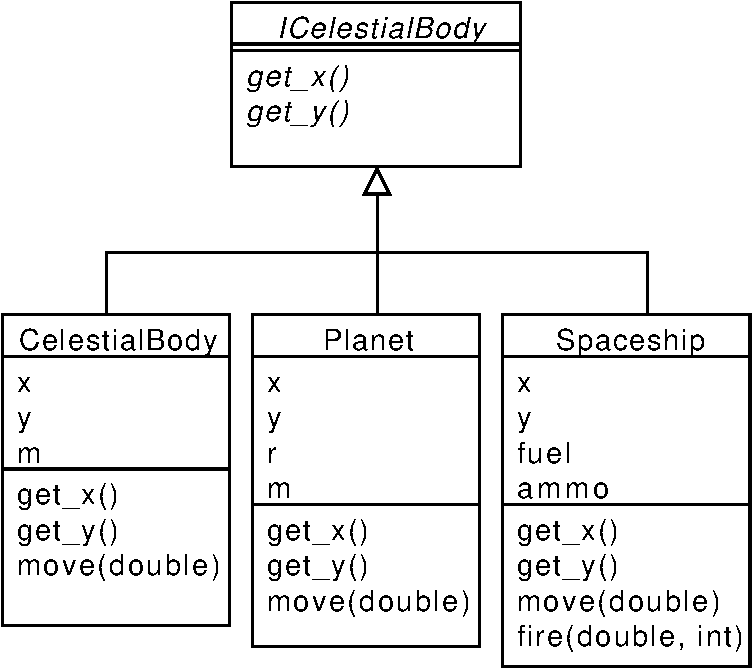
\includegraphics[width=0.8\textwidth]{illustrations/intf-inheritance-crop.pdf}
\caption{Открытое наследование интерфейса}
\label{fig:inheritance-interface}
\end{figure}

Теперь можно писать довольно абстрактный код, использующий приведение указателя или ссылки на объект, к указателю или ссылке на его открытый интерфейс. Как обычно сначала полезно написать небольшую служебную функцию:

\begin{lstlisting}
int 
in_between (double x, double ymin, double ymax)
{
  return (x <= ymax) && (x >= ymin);
}
\end{lstlisting}

И определить

\begin{lstlisting}
int 
Planet::detect_collision (const ICelestialBody &rhs) const
{
  return in_between (rhs.get_x(), x - r, x + r) && 
         in_between (rhs.get_y(), y - r, y + r);
}
\end{lstlisting}

Совершенно неважно с чем может произойти столкновение, если это ``что-то'' поддерживает все методы \lstinline!ICelestialBody!:

\begin{lstlisting}
Planet Jupiter;
Planet Earth;
CelestialBody Gallea;
/* .. */

Earth.detect_collision(Jupiter); 
Earth.detect_collision(Gallea);
\end{lstlisting}

Это похоже на общий разъём розетки, куда в стандартный интерфейс можно подключить много разных уcтройств (рис. \ref{fig:common-intf}).

\begin{figure}[ht]
\centering
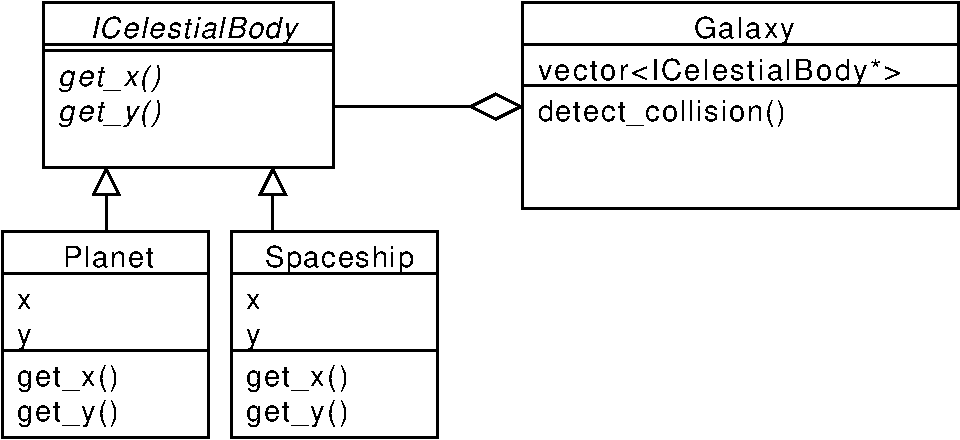
\includegraphics[width=1.0\textwidth]{illustrations/common-intf-crop.pdf}
\caption{Открытый интерфейс как общий разъём для подключения}
\label{fig:common-intf}
\end{figure}

Аргумент \lstinline!rhs! передан по константной ссылке. В принципе, он мог бы быть передан и по обычной ссылке и по (константному) указателю:

\begin{lstlisting}
int 
Planet::detect_collision (const ICelestialBody *rhs)
{
  return in_between (rhs->get_x(), x - r, x + r) && 
         in_between (rhs->get_y(), y - r, y + r);
}
\end{lstlisting}

По понятным причинам в случае абстрактного базового класса, аргумент не может быть передан по значению, так как не может быть сконструирован объект такого типа.

\subsubsection{Статический и динамический тип\index{Dynamic type}}\label{StatDynPoly}

Функция \lstinline!Planet::detect_collision! вызывает внутри себя виртуальную функцию \lstinline!ICelestialBody::get_x()! которая имеет один неявный аргумент -- указатель \lstinline!this! того объекта, для которого она вызвана. Этот указатель протягивается через формальный аргумент. 

Что можно сказать об аргументе \lstinline!rhs!? Всего лишь, что его тип, объявленный в списке аргументов (иначе говоря статический тип) это константная ссылка на \lstinline!ICelestialBody!. Это всё, что компилятор может сказать об этом типе \textbf{статически}, без контекста исполнения.

Но \textbf{динамически}, при вызове из \lstinline!main!, функция \lstinline!detect_collision! вызывается из двух разных мест с двумя разными параметрами, один из которых имеет тип \lstinline!Planet!, другой – тип \lstinline!CelestialBody! и именно эти типы имеет указатель \lstinline!this! для которого вызывается \lstinline!get_x()! в первом и во втором случае.

При вызове функции, она должна быть верно связана с именем типа, поскольку имя типа участвует в манглированном имени функции, как это объяснялось в (\ref{NameResolution}). При обычном вызове функции или метода, она связывается со своим типом статическим или ранним связыванием. Динамическое или позднее связывание работает при вызове виртуальной функции по ссылке или указателю на интерфейс. При этом решение о том какая функция в действительности будет вызвана, откладывается до момента вызова и принимается на основании её динамического типа. Обычно это требует дополнительного уровня косвенности для вызова через таблицу виртуальных методов, которая будет рассмотрена в (\ref{VirtualUnderHood}).

Если при динамическом связывании, функция имеет аргумент, который может принимать значения разных динамических типов с которыми она вызвана, этот аргумент называется \textbf{полиморфным} аргументом для динамического полиморфизма, а сама функция -- полиморфной (динамически полиморфной) функцией. В случае любой виртуальной функции единственный её полиморфный аргумент -- неявный указатель на объект, для которого она вызвана.

Вообще говоря, динамический тип может быть разрешен и в абстрактный класс. При этом производится попытка прямого вызова чисто виртуальной функции. Это ошибка, но язык C++ всегда даёт программисту возможность выстрелить себе в ногу, это фирменный стиль. Поэтому важно знать тот случай, когда это наиболее часто может произойти.

\subsubsection{Подробнее о чисто виртуальных функциях}\label{VirtualUnderHood}

Чтобы понять, что именно делает компилятор для того, чтобы вызов по указателю на интерфейс делегировался верному динамическому типу, полезно попробовать написать нечто подобное на C.

Сначала определяется таблица виртуальных методов

\begin{lstlisting}
typedef double (get_t)(void *);

struct celestial_body_vmt
{
  get_t *pget_x;
  get_t *pget_y;
/* ... */
};
\end{lstlisting}

Дальше указатель на эту таблицу идёт в структуру интерфейса:

\begin{lstlisting}
struct icelestial_body
{
  struct celestial_body_vmt vtable;
  /* ... */
};
\end{lstlisting}

Инициализация VMT происходит в конструкторе интерфейса:

\begin{lstlisting}
void
icelestial_ctor(struct icelestial_body *ths, get_t *pget_x, get_t *pget_y)
{
  ths->vtable.pget_x = pget_x;
  ths->vtable.pget_y = pget_y;
  /* ... */
}
\end{lstlisting}

Каждый класс-наследник содержит в себе интерфейсную часть и собственную реализацию интерфейсных функций:

\begin{lstlisting}
struct celestial_body
{
  struct icelestial_body intf;
  double x, y;
  /* ... */
};

double celestial_get_x(void *ths) { return ((struct celestial_body *)ths)->x; }
double celestial_get_y(void *ths) { return ((struct celestial_body *)ths)->y; }
\end{lstlisting}

Конструктор класса-наследника устанавливает известные ему функции в таблицу виртуальных функций интерфейсного класса:

\begin{lstlisting}
void 
celestial_ctor(struct celestial_body *ths)
{
  icelestial_ctor (&ths->intf, &celestial_get_x, &celestial_get_y);
  /* ... */  
}
\end{lstlisting}

Теперь всё готово для того, чтобы правильно сконструированный объект наследника мог участвовать в обобщённом коде наподобие уже рассмотренного collision detection (для простоты можно не рассматривать детали планет, имеющих некий радиус, а принять столкновение двух небесных тел как прохождение их на расстоянии epsilon):

\begin{lstlisting}
int
detect_collision (struct icelestial_body *lhs, struct icelestial_body *rhs)
{
  double x = lhs->vtable.pget_x(lhs);
  double y = lhs->vtable.pget_y(lhs);
 
  return in_between (rhs->vtable.pget_x(rhs), x - epsilon, x + epsilon) && 
         in_between (rhs->vtable.pget_y(rhs), y - epsilon, y + epsilon);
}
\end{lstlisting}

Вызов этого кода требует конструирования (вручную, поскольку используется C). Крайне многословный код, но так бывает всегда в недосахаренных системах.

\begin{lstlisting}
struct celestial_body Gallea;
struct celestial_body Encke;

celestial_ctor (&Gallea);
celestial_ctor (&Encke);

/* ... */

detect_collision (&Gallea.intf, &Encke.intf);
\end{lstlisting}

Таким образом, очевидно насколько много компилятор C++ прячет под капот. Знание механики работы виртуальных функций необязательно, но часто и очень сильно помогает. Например теперь ясно, что если бы передача параметров внутрь \lstinline!detect_collision! шла по значению, то они должны были быть сконструированы внутри функции. Но поскольку у \lstinline!icelestial_body! нет собственных координат и нет методов, чтобы их вернуть, то единственное, что можно передать в такой конструктор это нули:

\begin{lstlisting}
int
detect_collision (struct icelestial_body lhs, struct icelestial_body rhs)
{
  double x, y;
  
  icelestial_ctor (&lhs, 0, 0);
  icelestial_ctor (&rhs, 0, 0);

  x = lhs->vtable->pget_x();
  y = lhs->vtable->pget_y();
 
  return in_between (rhs->vtable->pget_x(), x - epsilon, x + epsilon) && 
         in_between (rhs->vtable->pget_y(), y - epsilon, y + epsilon);
}
\end{lstlisting}

И тогда вызов чисто виртуальной функции превращается в аналог вызова функции по нулевому указателю. При передаче же по указателю происходит всего лишь его приведение к указателю другого типа, без потери данных. Подобным образом работает и передача по ссылке в C++. Есть ещё несколько поучительных уроков: наличие дополнительного расхода памяти в каждом объекте на таблицу виртуальных функций, наличие дополнительной косвенности по вызову, ухудшение возможностей компилятора для инлайн-подстановки довольно простых методов и так далее -- всё это очевидно при понимании того, как вещи функционируют на самом деле.

Теперь самое время разобрать несколько хитрых вопросов, относящихся к наследованию интерфейса:

\subsubsection{Параметры по умолчанию\index{default arguments}}\label{DefArguments}

Тонкий вопрос, который многие программисты на C++ часто упускают из виду это то, как ведут себя виртуальные функции с параметрами по умолчанию. Если параметр по умолчанию в интерфейсе изменён в одном из его наследников:

\begin{lstlisting}
struct ICelestialBody
{
/* ... */
  virtual int apply_force (double f, double dt = 0.1) = 0;
};

void 
forcesApply (ICelestialBody *pbody, double *pfs, int n)
{
  for (; n > 0; --n)
    pbody->apply_force(pfs[n - 1]);
}

class CelestialBody: public ICelestialBody
{
public:
/* ... */
  int apply_force (double f, double dt = 0.01);
};
\end{lstlisting}

После чего этот обобщённый код вызван для конкретного динамического типа:

\begin{lstlisting}
double fs[5] = {1.0, 1.5, 1.2, 1.8, 1.10};
CelestialBody t;
forcesApply (&t, fs, 5);
\end{lstlisting}

Казалось бы -- реально будет вызвана функция \lstinline!apply_force! из класса \lstinline!CelestialBody! и логично ожидать значение аргумента по умолчанию таким, как он выставлен там. Но в реальности эта функция будет вызвана со значением аргумента по умолчанию, выставленным в интерфейсе.

Дело в том, что функции в C++ связываются динамически, а аргументы по умолчанию – статически. Если вернуться к сишному аналогу, можно легко увидеть, что в таблице виртуальных функций нет места для хранения и перезаписи аргументов по умолчанию.

\subsubsection{Виртуальные деструкторы}\label{VirtDestr}

Для программиста на C++ важно знать один очень специальный случай полиморфизма, относящийся к семантике освобождения, а именно виртуальные деструкторы. Рассмотрим пример – пусть у нас есть фабричная функция, которая в зависимости от радиуса желаемого пользователем небесного тела возвращает \lstinline!CelestialBody! если он меньше порогового значения или планету в другом случае:

\begin{lstlisting}
ICelestialBody *get_celestial_body (double r)
{
  if (r < epsilon)
    return new CelestialBody ();

  return new Planet ();
}
\end{lstlisting}

Что произойдёт если планета была получена через эту функцию, а потом удалена из памяти обычным способом?

\begin{lstlisting}
ICelestialBody *planet = get_celestial_body (100.0);
/* ... */
delete planet;
\end{lstlisting}

Будет освобождена базовая часть, но не будет освобождена производная часть, что неминуемо приведёт к утечкам памяти и проблемам. 

Решение этой проблемы: сделать деструктор виртуальным в интерфейсе. Тогда будет автоматически правильно вызван деструктор производного класса по указателю на базовый.

\begin{lstlisting}
struct ICelestialBody
{
  virtual double get_x () const = 0;
  virtual double get_y () const = 0;
  virtual int move (double dt) = 0;
  virtual int apply_force (double f, double dt) = 0;
  virtual ~ICelestialBody() {}
};
\end{lstlisting}

Наличие в классе невиртуального деструктора является в мире промышленного программирования достаточным основанием никогда ничего не наследовать от этого класса. Обратное – дурной тон. 

\subsubsection{Тела для чисто виртуальных функций}\label{VirtdestrBody}

\textbf{Вопрос к студентам:} можно ли объявить деструктор чисто виртуальным следующим образом:

\begin{lstlisting}
struct ICelestialBody
{
  /* ..... */
  virtual ~ICelestialBody() = 0;
};
\end{lstlisting}

\ifanswers
Правильный ответ: да, можно, но это приведет к pure virtual function call при попытке унчитожить любого наследника такого класса.
\fi

Тем не менее, иногда чисто виртуальный деструктор имеет смысл -- например если это единственная функция в интерфейсе. Выход: написать тело для чисто виртуального деструктора

\begin{lstlisting}
virtual ICelestialBody::~ICelestialBody()
{
}
\end{lstlisting}

В том случае, если у чисто виртуальной функции существует тело, эта функция всё ещё не может быть вызвана как метод своего класса, но она может быть вызвана из любого своего наследника.

\textbf{Вопрос к студентам:} как вы думаете зачем ещё может быть использована эта техника?

\ifanswers
Возможный ответ: для организации разумного поведения по умолчанию, которое наследники должны явно вызывать:

\begin{lstlisting}
class B 
{
public:
  virtual bool f() = 0;
};

bool 
B::f() 
{
  return true;  // this is a good default, but
}               // shouldn't be used blindly

class D : public B 
{
public:
  bool f() 
  {
    return B::f(); // if D wants the default
  }                // behaviour, it has to say so
};
\end{lstlisting}

Но тут возможны и другие варианты: например выдать лучшее сообщение об ошибке чем компилятор и выйти.
\fi

\subsubsection{Виртуальные конструкторы}\label{VirtCtors}

Статическая функция не может в общем случае быть ни виртуальной ни (тем более) чисто виртуальной. Поэтому конструкторы тоже не могут быть виртуальными.

\textbf{Вопрос к студентам:} а нужны ли нам вообще виртуальные конструкторы?

\ifanswers
Правильный ответ: да очень нужны. Скажем виртуальный конструктор копирования позволил бы создать в явном виде объект производного класса по указателю на объект базового класса
\fi

На этом нужно остановиться особо. Было упомянуто (см. \ref{RAII}), что для RAII фундаментальные переопределяемые функции это конструктор копирования и оператор присваивания. И вдруг оказывается, что второй может быть виртуальным, а первый никак:

\begin{lstlisting}
class IVector
{
public:
  virtual IVector& operator= (const IVector &rhs) = 0; // OK
  virtual IVector(const IVector *rhs) = 0; // ERROR
};
\end{lstlisting}

Приходится выкручиваться. Обычно в рамках выкручивания люди заводят виртуальную функцию \lstinline!clone! для получения копии объекта производного класса по указателю на базовый класс:

\begin{lstlisting}
class IVector
{
public:
  virtual IVector* clone() = 0; // virtual ctor idiom
  virtual void operator+= (const IVector &lhs) = 0;
};

class Vector : public IVector
{
public: 
  Vector (const Vector &rhs); // copy ctor
  void operator+= (const IVector &lhs); // add any vector to given
  IVector *clone() {
    return new Vector(*this);
  }
};

class SparceVector : public IVector
{
public: 
  SparceVector (const SparceVector &rhs); // copy ctor
  void operator+= (const IVector &lhs); // add any vector to given
  IVector *clone() {
    return new SparceVector(*this);
  }
};
\end{lstlisting}

Теперь общий код для сложения, которое поддерживает как обычные так и разреженные вектора можно реализовать в терминах виртуальных конструкторов:

\begin{lstlisting}
IVector *add (const IVector &rhs, const IVector &lhs)
{
  IVector &result = *rhs.clone();
  result += lhs;
  return &result;
}
\end{lstlisting}

Эта идиома крайне полезна и возмещает очевидный недостаток языка C++ в части виртуального конструирования.

\textbf{Вопрос к студентам:} но почему такой недостаток вообще есть? Что мешает сделать в языке настоящие виртуальные конструкторы?

\ifanswers
Правильный ответ: именно конструктор делает ту работу, которая должна быть сделана чтобы заработал механизм виртуальных функций. Поэтому в конструкторе класса виртуальные вызовы работают как не виртуальные. Поэтому даже если бы можно было сделать конструктор виртуальным, его вызов все равно был бы вызовом невиртуальной функции.
\fi

\pagebreak
\subsection{Наследование реализации}\label{ImplInheritance}

\hfill\textit{The object-oriented version of 'Spaghetti code' is,}

\hfill\textit{of course, 'Lasagna code'}{\vspace{0.5em}}

\hfill\textit{-- Roberto Waltman}

Разработанные в (\ref{PureVirtual}) классы-наследники \lstinline!CelestialBody! и \lstinline!Planet! всё ещё имеют слишком много дублирующегося кода: общие поля координат и скоростей, общие и притом идентичные селекторы координат. Это обычная и, более того, достаточно частая ситуация. Для уменьшения дублирования в классе \lstinline!Planet!, можно заметить, что планета также \textbf{является} небесным телом, отличаясь только тем, что у неё имеет значение радиус и есть дополнительный метод для определения столкновений. Это отношение ``быть частным случаем'' также, как и отношение ``реализовать интерфейс'' моделируется открытым наследованием, но в данном случае унаследована будет и реализация некоторых методов и поля класса \lstinline!CelestialBody!, такие как \lstinline!x! и \lstinline!y!. Общий интерфейс тот же:

\begin{lstlisting}
struct ICelestialBody
{
  virtual double get_x () const = 0;
  virtual double get_y () const = 0;
  virtual int move (double dt) = 0;
  virtual int apply_force (double f, double dt) = 0;
  virtual ~ICelestialBody() {}
};
\end{lstlisting}

Пользовательский тип \lstinline!CelestialBody! всё так же реализует общий интерфейс:

\begin{lstlisting}
class CelestialBody: public ICelestialBody
{
protected:
  double x, y;
  double vx, vy;
  double m;
public:
/* ... */
/* ICelestialBody implementation */
  double get_x () const { return x; }
  double get_y () const { return y; }
  int move (double dt); 
  int apply_force (double f, double dt);
/* ... */
};
\end{lstlisting}

Новое ключевое слово \lstinline!protected! сообщает, что все помеченные им поля при открытом наследовании будут доступны производным классам.

Пользовательский тип \lstinline!Planet! сообщает, что является уточнением \lstinline!CelestialBody!:

\begin{lstlisting}
class Planet: public CelestialBody
{
  double r;
public:
  int detect_collision (const ICelestialBody &rhs) const;
};
\end{lstlisting}

Теперь есть необходимость определить расстояние между небесными телами. Соответствующий обобщённый код:

\begin{lstlisting}
double 
get_distance (const ICelestialBody &lhs, const ICelestialBody &rhs)
{
  double xdist = lhs.get_x() - rhs.get_x();
  double ydist = lhs.get_y() - rhs.get_y();

  return sqrt (xdist*xdist + ydist*ydist);
}
\end{lstlisting}

Вполне может быть вызван так:

\begin{lstlisting}
Planet Jupiter;
Planet Earth;

/* ... */

double d = get_distance (Jupiter, Earth);
\end{lstlisting}

Несмотря на то, что функций \lstinline!Planet::get_x! и \lstinline!Planet::get_y! попросту не существует, у класса \lstinline!Planet! тем не менее есть эти методы, унаследованные от класса \lstinline!CelestialBody!. Внутри функции \lstinline!Planet::get_distance!, динамический тип \lstinline!Planet! аргумента \lstinline!lhs! позволяет сделать вызов общей для \lstinline!Planet! и \lstinline!CelestialBody! функции, которая изменяет их общую открытую часть.

Существенное отличие открытого наследования от наследования интерфейса -- класс не только даёт обещание, что будет поддерживать тот или иной интерфейс, но ещё и заимствует у базового класса конкретную реализацию, оставляя себе только уточнение специфичных для себя методов. Эта техника существенно улучшает переиспользование кода и может быть в произвольной пропорции смешана с чисто абстрактными классами: например вполне можно было бы внести координаты и их селекторы в интерфейсный класс, у которого в этом случае появилась бы часть интерфейса который наследники должны реализовать (чисто виртуальные функции) и часть реализации, которая просто наследуется для использования. Впрочем смешивать такие вещи -- не всегда полезно.

Теперь UML-диаграмма становится несколько более иерархичной, как показано на (рис. \ref{fig:inheritance-implementation}).

\begin{figure}[h!]
\centering
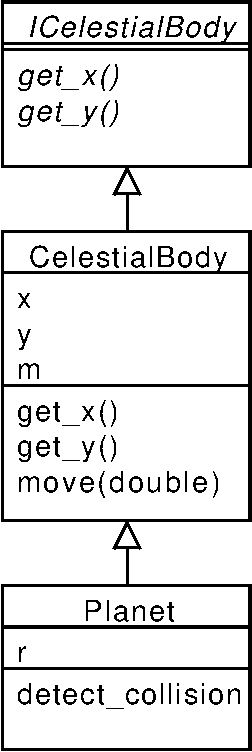
\includegraphics[width=0.3\textwidth]{illustrations/impl-inheritance-crop.pdf}
\caption{Открытое наследование реализации}
\label{fig:inheritance-implementation}
\end{figure}

Можно заметить, что сверху вниз по этой диаграмме, более общие понятия предшествуют более частным. Скажем ``конкретное небесное тело'' это ``небесное тело вообще'', а планета это и то и другое. При открытом наследовании все открытые члены базового класса доступны как открытые члены производного класса, а также работает неявное преобразование типа от производного к базовому классу. Говорят, что открытое наследование \textbf{моделирует} отношение ``is-a'', при котором объект производного класса является объектом базового класса (в том смысле, в каком планета является небесным телом). Это отношение довольно важно, подробнее см. (\ref{LSP}).

Увы, с точки зрения ООП на C++ такая диаграмма имеет фундаментальный и очевидный недостаток: конкретный класс \lstinline!CelestialBody! является базовым при наследовании. Это может привести к одной неприятной проблеме.

\subsubsection{Проблема срезки\index{Cutting}}\label{Cutting}

Можно ещё раз рассмотреть функцию \lstinline!detect_collision!, на этот раз остановившись на её параметрах. В диаграмме (рис. \ref{fig:inheritance-implementation}) не очевидно, что там должен стоять указатель на \lstinline!ICelestialBody!. Кажется достаточно простого указателя на \lstinline!CelestialBody! -- в конце концов это по факту общий интерфейс для всех объектов у которых можно запросить координаты.

Увы, это делает возможным передачу аргументов по значению.

\begin{lstlisting}
Planet::detect_collision (const CelestialBody rhs) /* Oops */
\end{lstlisting}

Проблема понятна: формальные аргументы, переданные по значению конструируются при входе в функцию. Попытка сконструировать объект абстрактного класса (то есть класса, содержащего хотя бы один чисто виртуальный метод) сама по себе ошибочна. Но здесь компилятор уже не защищает от такого ошибочного конструирования. В этом случае новосконструированный объект \lstinline!rhs! будет иметь динамический тип \lstinline!ICelestialBody! независимо от динамического типа аргументов. В этом случае вызов функции \lstinline!get_x()! будет связан с чисто виртуальной заглушкой интерфейса и в лучшем случае программа выйдет по ошибке. 

Этот срез информации при передаче по значению называется ``проблемой срезки''. Срезка часто возникает в практических контекстах и важно о ней помнить.

\subsubsection{Идиома NVI и разделение обязанностей}\index{NVI}\label{NVI}

Одним из способов бороться с проблемой срезки и одновременно сохранить наследование реализации может быть вынесение большинства функциональности и даже полей в абстрактный базовый класс, как показано на (рис. \ref{fig:better-implinhh})

\begin{figure}[h!]
\centering
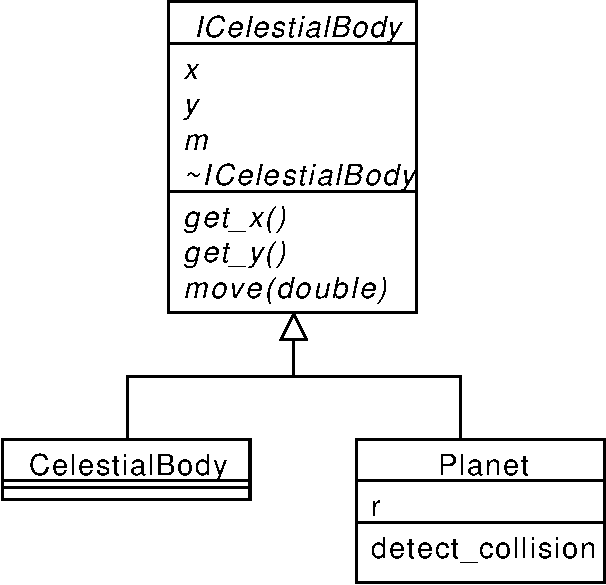
\includegraphics[width=0.7\textwidth]{illustrations/better-implinh-crop.pdf}
\caption{Способ делать конкретными классами только листья}
\label{fig:better-implinhh}
\end{figure}

\textbf{Домашняя наработка:} напишите код к этой UML-диаграмме

Делать конкретными классами только листья -- совет который разделяют многие авторы, для примера можно указать Майерса \cite{effcpp3d}.

Но такой подход порождает проблемы: функция \lstinline!get_x! больше не требует переопределения в наследниках (все ещё допуская его) и поэтому кто-то может забыть её переопределить, получив при этом странное поведение по умолчанию. Здесь уместен известный анекдот про кенгуру в программе-тренажере для летчиков (класс кенгуру был для простоты и от нехватки времени унаследован от класса пехотинец с соответствующими последствиями во время работы программы -- пилоты были поражены тактической слаженностью кенгуру а так же попытками стаи кенгуру запустить по самолету ``стингер'').

Выходом является разделить обязанности предоставления поведения по умолчанию и заглушки для переопределения:

\begin{lstlisting}
struct ICelestialBody
{
public:
  /* Non-Virtual interface */
  double get_x () const { return do_get_x(); }
  double get_y () const { return do_get_y(); }
  virtual ~ICelestialBody() = 0 {}

protected:
  double m_x, m_y;

private:
  virtual double do_get_x () = 0 { return m_x; }
  virtual double do_get_y () = 0 { return m_y; }
};
\end{lstlisting}

\textbf{Домашняя наработка:} нарисуйте UML-диаграмму с планетами и небесными телами к этому коду.

Эта идиома называется NVI (non-virtual interface) и крайне полезна. Один из таких полезных случаев будет рассмотрен далее, в (\ref{NameHiding}).

\subsubsection{Тонкости скрытия имён}\label{NameHiding}

При наследовании реализации имена имеют значение. Если некий класс \lstinline!Matrix! определяет две версии \lstinline!pow! (для возведения в целую степень, что гораздо проще и в вещественную, что сложнее):

\begin{lstlisting}
class Matrix
{
public:
  virtual void pow(int x);
  virtual void pow(double x);
};
\end{lstlisting}

То какой-то его наследник может решить переопределить только одну из них:

\begin{lstlisting}
class SparceMatrix : public Matrix
{
public:
  void pow (int x);
};
\end{lstlisting}

Увы, это плохая идея. При следующем вызове:

\begin{lstlisting}
SparceMatrix t;
/* ..... */
t.pow(5.0);
\end{lstlisting}

Произойдёт вовсе не вызов \lstinline!Matrix::pow(double)! а вместо этого неявное преобразование типа и вызов \lstinline!SparceMatrix::pow(int)!. Чтобы избежать такого поведения можно явно ввести имя базового класса в контекст производного класса:

\begin{lstlisting}
class SparceMatrix : public Matrix
{
public:
  using Matrix::pow;
  void pow (int x);
};
\end{lstlisting}

Либо можно воспользоваться идиомой NVI и переопределять закрытые функции с разными именами:

\begin{lstlisting}
class Matrix
{
public:
  /* Non-virtual interface */
  void pow(int x) { do_pow_int(x); }
  void pow(double x) { do_pow_dbl(x); }
private:
  virtual void do_pow_int(int x);
  virtual void do_pow_dbl(double x);
};
\end{lstlisting}

Здесь снова разделяется поведение по умолчанию и заглушки для переопределения.

\subsubsection{Закрытое и защищенное наследование}\label{OtherInheritance}

Существенно иначе обстоят дела с закрытым наследованием. При закрытом наследовании, неявного преобразования типа от производного к базовому не задаётся, а все открытые методы базового класса становятся закрытыми методами производного класса, как показано в таблице ниже:

\begin{center}
  \begin{tabular}{ | l | c | c | r | }
    \hline
    modifier & public & protected & private \\ \hline \hline
    public & public & protected & private \\ \hline
    protected & protected & protected & private \\ \hline
    private & private & private & private \\ \hline
  \end{tabular}
\end{center}

Важно понимать, что в эту таблицу сведена внешняя видимость полей и методов класса. Внутрення видимость и видимость для наследников остаётся прежней.

Говорят, что закрытое наследование моделирует отношение part-of (быть частью). В принципе у закрытого наследования нет почти никакой разницы с композицией:

\begin{lstlisting}
struct Engine
{
  int start() const;
};
\end{lstlisting}

Теперь этот двигатель может быть включен в космический корабль посредством композиции

\begin{lstlisting}
class SpaceShip_p
{
  Engine e;
public:
  int start (double dt) const { e.start(); } 
};
\end{lstlisting}

Или же посредством закрытого наследования.

\begin{lstlisting}
class SpaceShip_p: private Engine
{
public:
  int start (double dt) const { Engine::start(); }
};
\end{lstlisting}

Впрочем одна тонкая разница будет видна при разговоре о множественном наследовании.

Защищенное наследование не слишком популярно в C++, однако автору удалось найти одно интересное применение (вынесено в тест по этой части курса).

\subsubsection{Конструкторы базовых классов}\label{BaseClassConstr}

При конструировании каждого класса будут неявно вызваны конструкторы его базовых классов по умолчанию, если они не вызваны явно в списке инициализации. Если эти конструкторы нетривиальные, то они, соответственно \textbf{должны} быть явно вызваны в списке инициализации:

\begin{lstlisting}
class A
{
  int x_;
public:
  A(int x) : x_(x) {}
};

class B : public A
{
public:
  B() {} // error!
  B(int x) : A(x) {} // ok
};
\end{lstlisting}

Здесь ошибка при попытке дефолтной инициализации вызвана тем, что подобъект класса \lstinline!A! должен быть инициализирован, но нет.

Необходимо понимать, что время жизни объекта начинается после того, как отработал его конструктор. Это означает, что следующий код (хотя и корректен с точки зрения языка) не верен:

\lstinputlisting[firstline=1,lastline=12]{cpp_code/p2s7.cpp}

Здесь сразу две ошибки. Во-первых попытка вызвать метод \lstinline!f()! базового подобъекта, который ещё не сконструирован в этой точке (поскольку только вызывается его конструктор). Это может прокатить, может нет, но это в любом случае некорректно. Во-вторых попытка инициализировать и потом использовать ещё не существующий член производного класса (до конструирования которого там пока вообще далеко).

Не следует допускать таких ошибок в своём коде.

\subsubsection{Больше возможностей для полиморфизма}\label{NewVirtual}

Начиная с C++11 в язык было введено несколько дополнительных возможностей, которых часто действительно не хватало и которые будут рассмотрены ниже.

В разделе (\ref{NameHiding}) уже рассматривалась возможность неявных ошибок из-за разрешения имен в стиле C++. Теперь настало время рассмотреть ещё одну ошибку такого рода и что с этим делать. Итак, всё те же матрицы.

\begin{lstlisting}
struct Matrix
{
  virtual void pow(int x);
};
\end{lstlisting}

И тут программист совершает обычную человеческую ошибку.

\begin{lstlisting}
struct SparceMatrix : Matrix
{
  void pow (long x); // oops
};
\end{lstlisting}

Увы, эта функцию вовсе не перегружает исходную функцию \lstinline!pow! и в каком-нибудь сложном динамическом контексте могут быть неприятные сюрпризы. 

\begin{lstlisting}
Matrix *m = new SpaceMatrix;
// .....
m->pow(1); // calls Matrix::pow!
\end{lstlisting}

Действительно, разные сигнатуры засчитываются как разные функции, перегрузки не происходит, всё плохо. Застраховаться от таких ошибок помогает спецификатор \lstinline!override!.

\begin{lstlisting}
struct SparceMatrix : Matrix
{
  void pow (long x) override; // BOOM!
};
\end{lstlisting}

Теперь класс-наследник сообщает компилятору, что он хочет именно переопределять функцию из предка и спасительная ошибка компиляции оповещает, что что-то пошло не так. Это, пожалуй, самое полезное из нововведений 2011-го года и использование его обязательно для всех живых существ, которые не хотят проблем и неприятностей.

Ещё один спецификатор, тоже полезный в этом случае, но кроме того вообще запрещающий дальнейшее переопределение это \lstinline!final!.

\begin{lstlisting}
struct SparceMatrix : Matrix
{
  void pow (long x) final; // BOOM!
};
\end{lstlisting}

и одновременно

\begin{lstlisting}
struct SparceMatrix : Matrix
{
  void pow (int x) final; // Ok
};

struct MySparceMatrix : SparceMatrix
{
  void pow (int x) override; // BOOM!
};
\end{lstlisting}


Ещё одно ограничение языка -- невозможность запретить наследование тоже долго преследовало программистов. Долгое время действовало неформальное правило -- нельзя наследоваться если нет виртуального деструктора, но все очень любили его нарушать. К счастью, эту проблему тоже решает модификатор \lstinline!final!.

\begin{lstlisting}
struct Matrix final;
struct SparceMatrix : Matrix; // BOOM!
\end{lstlisting}

Использование \lstinline!final! служит непреодолимым барьером в абстракции, поэтому им не следует злоупотреблять, а следует применять только когда он необходим.

\pagebreak
\subsection{Множественное наследование}\label{MultipleInheritance}

\hfill\textit{The one indisputable fact about MI in C++}

\hfill\textit{is that it opens up a Pandora's box of complexities}

\hfill\textit{that simply do not exist under single inheritance}{\vspace{0.5em}}

\hfill\textit{-- Scott Meyers}

До сих пор рассматривалось только одиночное одноуровневое наследование, но C++ даёт в этом отношении гораздо больше свободы. Один класс может наследовать многим классам, которые сами кому-то наследуют и так далее. Для этого базовые классы с их модификаторами доступа перечисляются через запятую

\begin{lstlisting}
class Man: public AnimalsWithTwoLegs, public OnesWithoutWings {};
\end{lstlisting}

Это позволяет строить иерархии взаимодействующих классов и объектов при проектировании сложных программных систем.

\begin{figure}[h!]
\centering
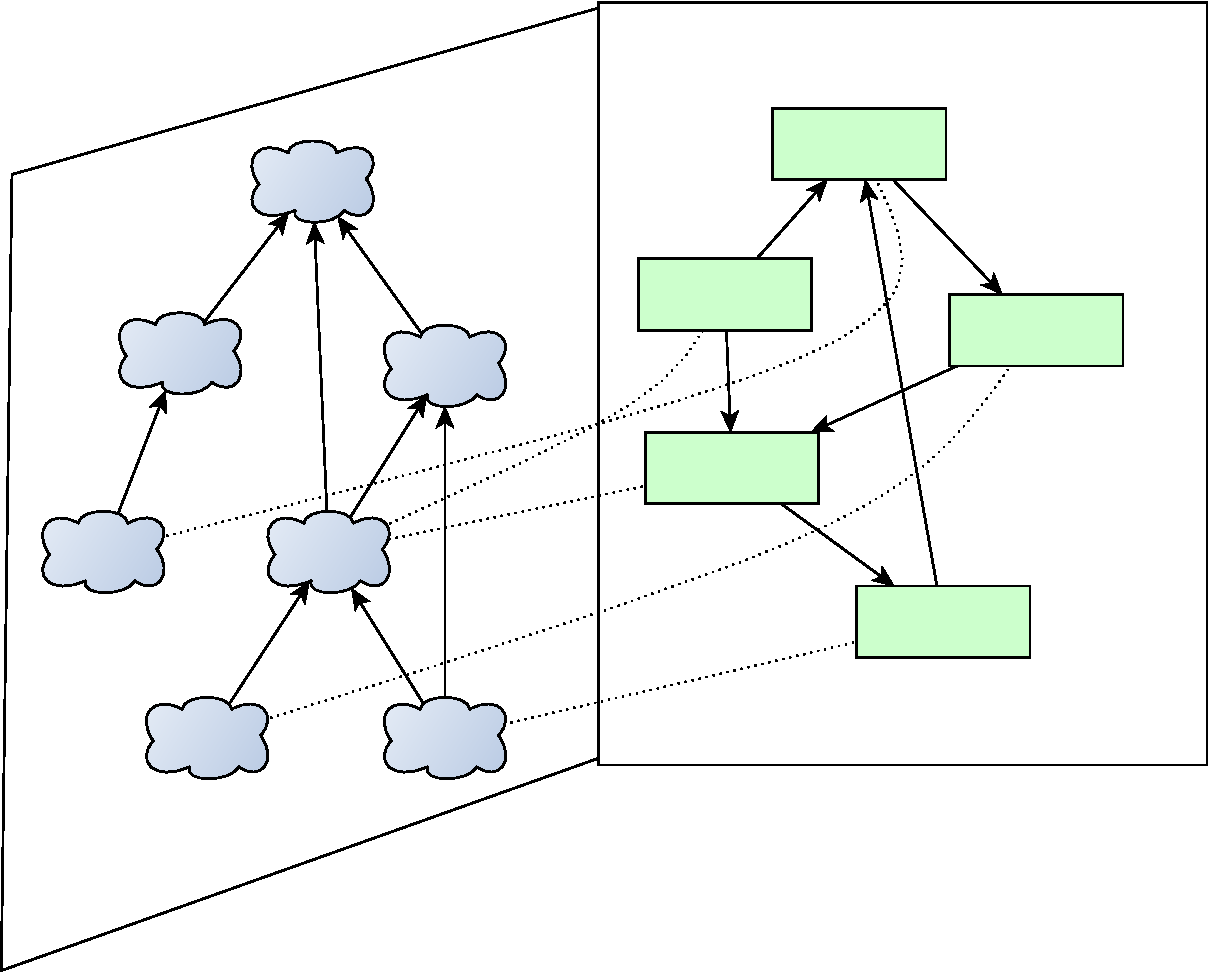
\includegraphics[width=0.8\textwidth]{illustrations/hierarchies-crop.pdf}
\caption{Иерархии классов и объектов}
\label{fig:hierarchies-crop}
\end{figure}

Проектирование хорошей иерархии это всегда сложный инженерный процесс, выходящий за рамки этого курса. Зато можно на игрушечных примерах рассмотреть основные проблемы, ожидающие разработчика на этом пути.

\subsubsection{Виртуальные функции при множественном наследовании}\label{VirtThunks}

При одиночном наследовании, отношение is-a, задаваемое открытым наследованием не вызывает проблем при использовании такой стандартной техники как таблицы виртуальных методов. На (рис. \ref{fig:multinh-crop}) изображена условная схема размещения в памяти объекта класса \lstinline!B!, определяемого как:

\begin{lstlisting}
class A { /* A part */ };
class B : public A { /* B part */ };
\end{lstlisting}

Видно, что указатель \lstinline!A*! в памяти указывает в точности туда же, куда \lstinline!B*! и одна и та же таблица виртуальных методов вполне достаточна.

\begin{figure}[h!]
\centering
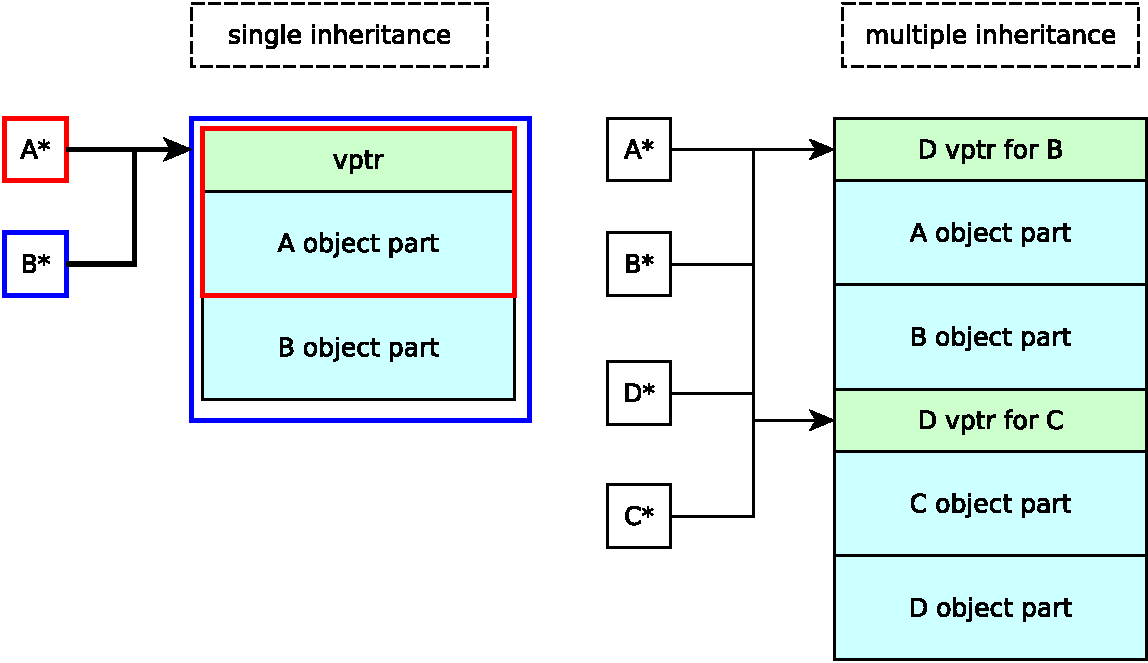
\includegraphics[width=1.0\textwidth]{illustrations/multinh-crop.pdf}
\caption{Виртуальные функции при множественном наследовании}
\label{fig:multinh-crop}
\end{figure}

Для прогулок по такой иерархии вполне достаточно статического приведения типа:

\begin{lstlisting}
B* ptrB = new B;
A* ptrA = ptrB;
ptrB = static_cast<B*>(ptrA);
\end{lstlisting}

Увы, для множественного наследования вечер резко перестаёт быть томным. Справа на (рис. \ref{fig:multinh-crop}) изображена ситуация, которая получается если добавить пару классов к иерархии:

\begin{lstlisting}
class C { /* C part */ };
class D : public B, public C { /* D part */ };
\end{lstlisting}

Даже если предположить, что две таблицы виртуальных функций будут совмещены, всё равно неясно куда должен показывать \lstinline!С*! если учесть, что в объекте после его разыменования или срезки просто не должно быть никаких частей от классов \lstinline!A! и \lstinline!B!, к которым он вообще не имеет отношения.

\begin{lstlisting}
D* ptrD = new D;
B* ptrB = ptrD;
A* ptrA = ptrD;
C* ptrC = ptrD; // Where to point?
\end{lstlisting}

К счастью стандарт регламентирует, что это не ваша головная боль, а головная боль компилятора. Компилятор статически знает, что при множественном наследовании преобразования некоторых типов на добавку постоянного смещения дороже, чем преобразования некоторых других типов (это безумие реализуется в бэкенде GCC через virtual function thunks -- специальные участки кода, в которых бэкенд решает сколько добавить к указателю при вызове виртуальной функции).

Теперь настало время разобраться с чем-то, что является \textbf{вашей} головной болью.

\subsubsection{Ромбовидные схемы и виртуальные базовые классы}\label{RombSchemas}

Предположим, вы проектируете систему, поддерживающую абстракции файлов ввода и вывода. Рано или поздно вы пришли к чему-то вроде такого

\begin{lstlisting}
class File {};
class InputFile : public File {};
class OutputFile : public File {};
class IOFile : public InputFile, public OutputFile {};
\end{lstlisting}

Графически это может быть выражено ромбовидной схемой

\begin{figure}[h!]
\centering
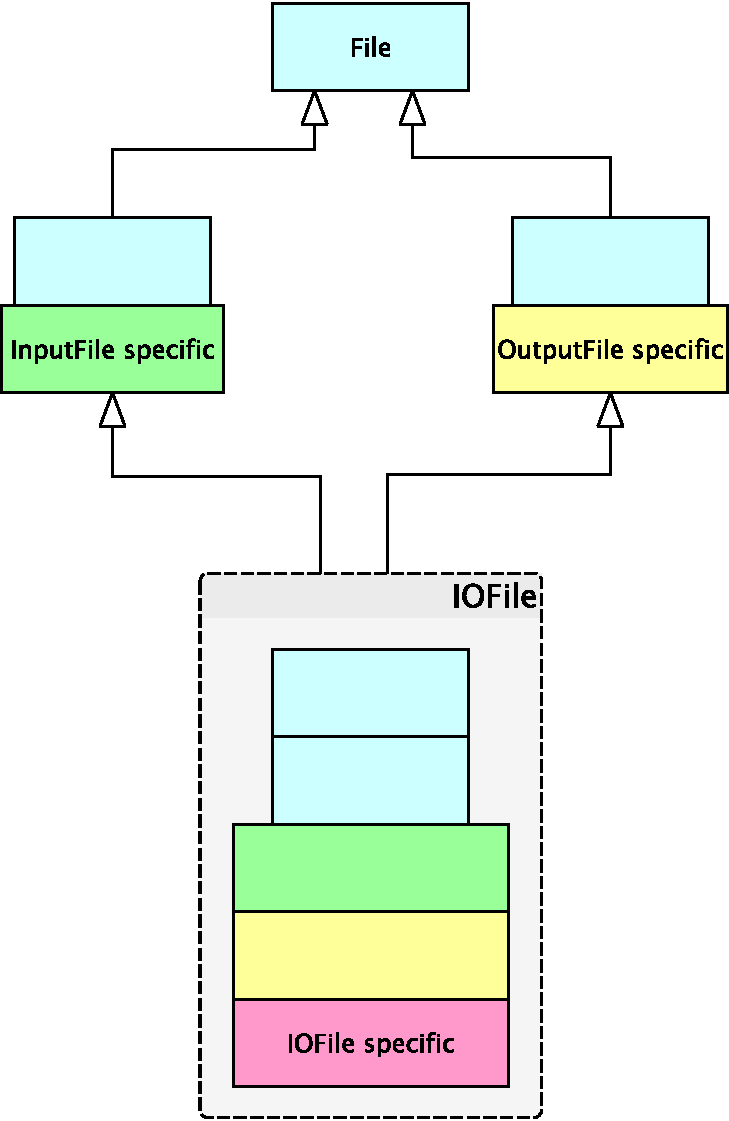
\includegraphics[width=0.5\textwidth]{illustrations/romb-crop.pdf}
\caption{Ромбовидная схема}
\label{fig:romb-crop}
\end{figure}

Предположим, что в классе \lstinline!File! есть поле \lstinline!File::filename!. По умолчанию, в классе \lstinline!IOFile! у вас получится два члена: \lstinline!InputFile::File::filename! и \lstinline!OutputFile::File::filename!, но файл у которого два имени это абсурд. 

Ещё хуже то, что отношение is-a похоже перестаёт работать в таких случаях:

\begin{lstlisting}
IOFile* iof = new IOFile;
File *f = iof; // Ooops!
\end{lstlisting}

Здесь абсолютно неясно на какую из двух частей \lstinline!InputFile::File! и \lstinline!OutputFile::File! теперь указывает \lstinline!f!. И вот это уже гораздо более серьёзная проблема, чем просто чуть больше оверхеда.

Прошаренный в C++ пацан предложил бы следующий disambiguation:

\begin{lstlisting}
File* outPtr = static_cast<OutputFile*>(iof);
File* inPtr = static_cast<InputFile*>(iof);
\end{lstlisting}

Но такие прекрасные хаки никак не спасают от фундаментальных проблем при вызове виртуальных функций. Если переопределение функции \lstinline!open! предлагается только классами \lstinline!File! и \lstinline!OutputFile!, что должно произойти при вызове \lstinline!inPtr->open!?

Чтобы избежать такой ситуации, базовый класс в наследовании может быть объявлен виртуальным (ещё можно вообще никогда ничего не писать на C++, а использовать C, это предпочтительный вариант).

\begin{lstlisting}
class File {};
class InputFile : virtual public File {};
class OutputFile : virtual public File {};
class IOFile : public InputFile, public OutputFile {};
\end{lstlisting}

Теперь всё хорошо и в ромбовидной схеме у самого нижнего производного класса есть только одна копия базового. В памяти это может выглядеть как-то так:

\begin{figure}[h!]
\centering
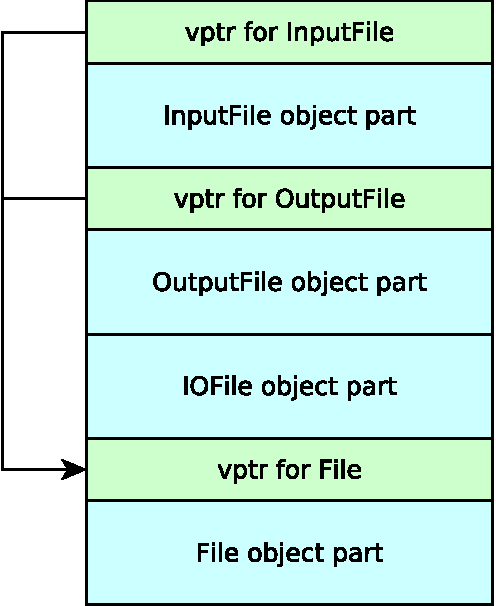
\includegraphics[width=0.5\textwidth]{illustrations/virtualinh-crop.pdf}
\caption{Виртуальное наследование}
\label{fig:virtualinh-crop}
\end{figure}

Таблицы виртуальных методов ещё более усложнились. Показанные стрелки позволяют во время исполнения как бы ``склеивать'' подобъекты, получая указатели на них.

\begin{lstlisting}
File* ptrF1 = ptrInputFile;
File* ptrF2 = ptrOutputFile;
File* ptrF3 = ptrIOFile;
\end{lstlisting}

Всё это будет работать и возвращать правильные (по крайней мере -- правильно себя ведущие) указатели. Увы, любое обращение по такому указателю связано уже с тремя уровнями косвенности: разрешение виртуального наследования, разрешение множественного наследования и далее собственно вызов по косвенности виртуального метода. Это указатель на указатель на указатель на функцию и, обычно, это высокий барьер для оптимизаций в компиляторе.

Ещё одна проблема -- виртуальное наследование отключает понижающие статические преобразования:

\begin{lstlisting}
IOFile* ptrIO = static_cast<IOFile*>(ptrF3); // Error
\end{lstlisting}

\textbf{Вопрос к студентам:} почему это происходит?

\ifanswers
Правильный ответ: потому что для реконструкции объекта с виртуальным наследованием, компилятор должен пройти по каждой из возможных цепочек виртуального наследования и создать каждый из подобъектов. Это неконстантный оверхед по времени и памяти и разработчики языка не стали его закладывать в обычное преобразование.
\fi

Для того, чтобы выполнять понижающее преобразование, следует воспользоваться специально введенным для этого в язык динамическим приведением типа.

\subsubsection{Динамическое приведение\index{dynamic\_cast} и RTTI\index{RTTI}}\label{DynCastRTTI}

Кроме всех операторов приведения, рассмотренных в (\ref{FromCCastToCPP}), существует ещё один, разработаный специально, чтобы приводить статический тип к динамическому типу. Он называется \lstinline!dynamic_cast!. 

Его интересной особенностью является то, что он по-разному работает для указателей и для ссылок. 

Для указателей

\begin{lstlisting}
Derived* temp = dynamic_cast<Derived*>(base);
\end{lstlisting}

Пытается привести p, типа \lstinline!Base*! к типу \lstinline!Derived*!, где \lstinline!Base! и \lstinline!Derived! принадлежат одной и той же иерархии. Если \lstinline!Derived! является базовым классом для \lstinline!Base!, то это ничем не отличается от \lstinline!static_cast!. Но \lstinline!dynamic_cast! работает также если Base является полиморфным базовым классом для \lstinline!Derived!, то есть является базовым классом для \lstinline!Derived! и содержит виртуальные функции. Звучит запутано? Давайте посмотрим пример.

\lstinputlisting{cpp_code/p2s13.cpp}

Что будет на выдаче? Ответ:

\begin{verbatim}
You are Dart Veider!
You are not Dart Veider, you are Pokemon
\end{verbatim}

Коротко говоря, \lstinline!dynamic_cast!, использованый для указателя даёт возможность ``спросить'' такой ли у этой переменной динамический тип, как он полагает. Он приводит к этому типу если ответ ``да'' или возвращает \lstinline!NULL!, если ответ ``нет''.

При использовании \lstinline!dynamic_cast! для ссылок, вопрос превращается в утверждение. Если это утверждение нарушается, кидается исключение, подробнее про исключения речь пойдет в (\ref{CppExceptions}).

\textbf{Вопрос к студентам:} может ли \lstinline!dynamic_cast! работать везде, где работает \lstinline!static_cast!?

\ifanswers
Правильный ответ: нет \lstinline!dynamic_cast! очень важно, чтобы в базовом классе была хотя бы одна виртуальная функция -- если таблицы виртуальных методов не будет существовать, динамическое приведение не будет работать.
\fi

Именно такой вид преобразования является законным понижающим преобразованием в виртуальных иерархиях.

\begin{lstlisting}
IOFile* ptrIO = dynamic_cast<IOFile*>(ptrF3); // Ok
\end{lstlisting}

Важно понимать: любое использование \lstinline!dynamic_cast! это легальный способ попросить компилятор сделать вашу программу гораздо медленнее и несколько больше по размеру. Дело в том, что для своей работы он использует запросы к так называемой run time type information или RTTI -- обычно это структура, привязанная к виртуальной таблице. Измерить (или хотя бы оценить) точный оверхед обращения к этой структуре и её хранения невозможно. Считается, что если вы используете \lstinline!dynamic_cast!, вы знаете что делаете.

Из опыта автора этих лекций, обычно люди, использующие его, вообще не знают что делают. Даже примерно.

\subsubsection{Информация о типах и идентификаторы типов\index{type\_info}}\label{TypeInfo}

Каждому типу в C++ соотнесен дескриптор, имеющий тип \lstinline!type_info!. Этот дескриптор для любого типа можно получить вызвовом функции \lstinline!typeid!. Такие объекты содержащие информацию о динамических типах можно сравнивать. Можно также, начиная с 2011, сравнивать их хеш-коды.

Таким образом, есть два варианта сравнения совпадает ли динамический тип с заданным.

\begin{enumerate}

\item Использовать dynamic cast

\begin{lstlisting}
if (dynamic_cast<A*> someVar != 0) { 
  //it is of class A, or X, inherited from A 
}
\end{lstlisting}

\item Использовать typeid

\begin{lstlisting}
if (typeid(someVar) == typeid(A)) {
   //it is of class A
}
\end{lstlisting}

\end{enumerate}

Первый способ позволяет сравнить нечетко, динамический тип может быть приведен к \lstinline!A! из любого наследника. Во втором случае сравнение будет четким, а главное -- дешевым. Сравнить идентификаторы типов имеет постоянную сложность. Динамическое приведение типов требует обхода деревьев RTTI и может работать непредсказуемо долго.

\textbf{Вопрос к студентам:} зачем же вообще нужен \lstinline!dynamic_cast! если есть \lstinline!typeid!?

\ifanswers
Правильный ответ: в первую очередь из-за сложностей приведения в связке \lstinline!typeid! + \lstinline!static_cast! (см. выше разговор о том почему в иерархиях множественного наследования нам вообще не хватает статического приведения).
\fi

\subsubsection{Сюрпризы в конструкторах при виртуальном наследовании}\label{VirtualBaseClassConstr}

Пусть виртуальный базовый класс имеет нетривиальный конструктор как в (\ref{BaseClassConstr}).

\begin{lstlisting}
class A 
{
  int x_;
public:
  A(int x) : x_(x) {}
};
\end{lstlisting}

И является виртуальным базовым для классов:

\begin{lstlisting}
/* C is similar */
class B : virtual public A
{
public:
  B(int x):A(x){}
};
\end{lstlisting}

Увы, ожидаемый порядок конструирования для класса наследующего по ромбовидной схеме не сработает интуитивно:

\begin{lstlisting}
class D : public B, public C {
public:
  D(int x) : B(x), C(x) {} // Error!
}
\end{lstlisting}

Дело в том, что виртуальный базовый класс должен быть обязательно сконструирован в самом нижнем наследнике, то есть:

\begin{lstlisting}
  D(int x) : A(0), B(x), C(x) {} 
\end{lstlisting}

Мало того, подобъект A будет сконструирован именно с параметром 0, те параметры которые протакиваются через конструкторы подобъектов будут проигнорированы.

Это распространяется и ниже по иерархии туда, где об общем виртуальном предке все уже давно забыли:

\begin{lstlisting}
class E : public D {
public:
  E() : D(10) {} // Error!
};
\end{lstlisting}

Теперь самый нижний класс в иерархии внезапно \lstinline!E! и значит виртуально-базовая часть должна быть сконструирована в нем.

\subsubsection{Порядок инициализации в сложных диаграммах}\label{InitOrder}

Важно очень хорошо представлять себе порядок конструирования сложных диаграмм классов. Ниже приведен несколько синтетический (но на самом деле гораздо менее сложный, чем многие практически важные иерархии) пример.

\lstinputlisting[firstline=3,lastline=15]{cpp_code/p2s12.cpp}

Для простоты можно изобразить эту иерархию на листочке:

\begin{figure}[h!]
\centering
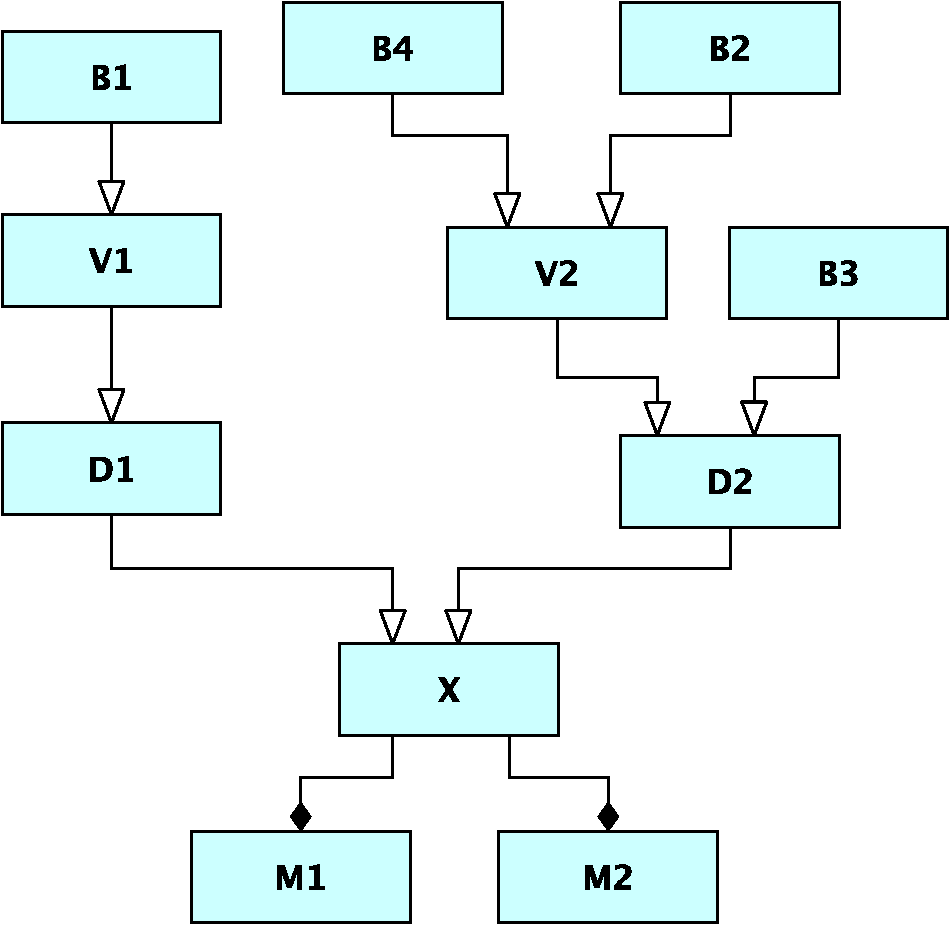
\includegraphics[width=0.5\textwidth]{illustrations/complexhier-crop.pdf}
\caption{Сложная иерархия}
\label{fig:complexhier-crop}
\end{figure}

Порядок инициализации объекта класса \lstinline!X! для изображённой иерархии следующий:

\begin{itemize}
\item Сначала конструируются виртуальные базовые классы
  \begin{enumerate}
  \item Конструирование \lstinline!V1!: \lstinline!B1::B1()!, \lstinline!V1::V1()!
  \item Конструирование \lstinline!V2!: \lstinline!B1::B1()!, \lstinline!B2::B2()!, \lstinline!V2::V2()!
  \end{enumerate}
\item Затем конструируются невиртуальные базовые классы
  \begin{enumerate}
  \item Конструирование \lstinline!D1!: \lstinline!D1::D1()!
  \item Конструирование \lstinline!D2!: \lstinline!B3::B3()!, \lstinline!D2::D2()!
  \end{enumerate}
\item Затем конструируются члены \lstinline!M1::M1()!, \lstinline!M2::M2()!
\item И в последнюю очередь выполняется конструктор \lstinline!X::X()!
\end{itemize}

Вид наследования (открытое, закрытое или защищённое) не влияет на порядок инициализации.

\subsubsection{Делегация сестринскому типу}

Сложности, вносимые множественным наследованием в механизм виртуальных функций, частично окупаются теми возможностями, которые они предоставляют.

Пусть задана ромбовидная иерархия, в которой виртуальная функция определена в одной, но не в другой ветке:

\begin{lstlisting}
struct VBase {
  virtual void foo () = 0;
  virtual void bar () = 0;
  virtual ~VBase () = 0 {}
};

struct Base1 : virtual public VBase {
  // do not override bar
  // but CALL it
  void foo() override { bar(); }  
};

struct Base2 : virtual public VBase {
  void bar() override {}
};

struct S : Base1, Base2 {}
\end{lstlisting}

На что может рассчитывать пользователь такого класса, вызывая метод \lstinline!foo! объекта класса \lstinline!S!?

\begin{lstlisting}
S x;
x.foo();
\end{lstlisting}

Происходит интересная вещь: поскольку \lstinline!foo! не переопределена в \lstinline!Base2!, будет без вариантов вызвана \lstinline!Base1::foo! из которой (!) будет вызвана \lstinline!Base2::bar!. Несмотря на то, что классы \lstinline!Base1! и \lstinline!Base2! находятся на одном уровне, механизм виртуальных функций позвоялет такие братские делегации.

\subsubsection{Вложенные классы и снова о пространствах имён}\label{InnerClasses}

Вложенные функции в C++ невозможны так же как и в C (что кстати не вполне логично, так как вложенные лямбда-функции в новом стандарте возможны и будут рассмотрены на следующих лекциях, так что казалось бы гулять так гулять). Зато C++ позволяет вкладывать классы. Синтаксис очевиден, но, если необходимо, чтобы вложенный класс ``знал'' о своём окружении, об этом надо позаботиться отдельно:

\lstinputlisting{cpp_code/p2s15.cpp}

Каждый вложенный класс определяет область видимости своих имён. Таким образом, можно создать отдельный объект типа \lstinline!DeathStar::DartVeider!, но можно и запретить это, поместив его в \lstinline!private!. Это существенное преимущество

\pagebreak
\subsection{Скажи мне кто твой друг}\label{WhosYourFriend}\index{Friend}

\hfill\textit{C++ : Where friends have access to your private members}{\vspace{0.5em}}

\hfill\textit{-- Gavin Russell Baker}

Модель инкапсуляции C++ логична и стройна (общий смех). В общем случае закрытые члены класса формируют его состояние и недоступны извне, иначе, чем через его методы, отражающие поведение -- это хорошо и правильно. Но в некоторых случаях, разработчик хотел бы дать некоему классу эксклюзивный доступ к закрытым членам другого класса. Например для того, чтобы не писать кучу геттеров и в то же время сохранить консистентность абстракции. Для этого язык C++ предусматривает механизм друзей (\lstinline!friend!) класса.

\subsubsection{Обычная дружба}

Наиболее типичным применением дружбы является дружба между классами. Для этого объявление класса, которому хочется открыть внутреннее состояние должно быть предварено ключевым словом \lstinline!friend!.

\begin{lstlisting}
class Node
{
  int data;
  int key;
  /* ..... */

  /* class BinaryTree can access data directly */
  friend class BinaryTree; 
};
\end{lstlisting}


Класс \lstinline!Node!, назначив себе друга \lstinline!BinaryTree!, открыл ему всё свое закрытое состояние, но, при этом, сам не получил никакого доступа к \lstinline!BinaryTree!. Теперь внутри BinaryTree можно написать код вида:

\begin{lstlisting}
class BinaryTree
{
  Node *root;

public:
  int find(int key);
};

int BinaryTree::find(int key)
{
  /* check root */
  if(root->key == key)
    {
      /* no need to go through an accessor function */
      return root->data;
    }
  /* rest of find */
}
\end{lstlisting}


Класс может открывать своё состояние не только классам, но и функциям. Скажем, не открывая доступ всему \lstinline!BinaryTree!, можно открыть его только методу \lstinline!find!:

\begin{lstlisting}
class Node
{
  int data;
  int key;
  /* ..... */

  /* BinaryTree::find can access data directly */
  friend int BinaryTree::find();
};
\end{lstlisting}

Открыть внутреннее состояние можно и отдельной функции. Как дополнительный плюс -- в этом случае функция считается объявленной.

\begin{lstlisting}
struct Node
{
  // declaration
  friend int find();
};


// find declared and can be used
int t = find();

// definition
int
find() 
{
  /* ..... */
}
\end{lstlisting}

Благодаря такому свойству объявлений, дружба может быть полезна во многих неожиданных контекстах при работе с шаблонами (см. \ref{BartonNackman}).

\subsubsection{Адвокат дружбе не помеха}

К сожалению, в языке не реализовано полноценное открытие части состояния. Семантика дружбы диктует ``все или ничего''. Но редко когда нужно, чтобы друзья имели доступ ко всему подряд. Пусть рассмотренный выше класс \lstinline!Node! согласен открыть классу \lstinline!BinaryTree! только свои поля \lstinline!data! и \lstinline!key!, оставив все остальные закрытыми. В этом случае классу \lstinline!Node! следует прибегнуть к услугам адвоката (английское слово attorney означает скорее ``поверенный'').

Игра слов дат название идиоме attorney-client (адвокат-клиент). Адвокат, которым мог бы обзавестить \lstinline!Node! может выглядеть вот так

\begin{lstlisting}
class NodeAttorney {
private:
  static int& data(Node &c) {
    return c.data;
  } 
  static int& key(Node &c) {
    return c.key;
  } 
  friend class BinaryTree;
};
\end{lstlisting}

Теперь внутри \lstinline!Node! можно оставить только объявление дружбы со своим адвокатом, прочие же объявления дружбы вынести в класс-attorney.

Особо параноидальный дизайн иерархии классов может предоставлять много адвокатов на каждое закрытое поле популярного клиента, каждого со своим списком пользователей.

Нужно очень хорошо понимать, что все эти игры свидетельствуют о наличии некоей проблемы между креслом и компьютером.

\subsubsection{Дружба в иерархиях классов}

Дружба не наследуется, но друг статического родительского типа достаточен, чтобы делать дружественные вызовы полиморфных наследников.

\lstinputlisting[firstline=51,lastline=80]{cpp_code/p2s16.cpp}

В общем случае, дружба статических типов вредна для инкапсуляции. Но дружба, позволяющая полиморфные вызовы по большой и закрытой иерархии это полезно и иногда необходимо. 

\subsubsection{Дружба и виртуальные вызовы}

Часто хочется, чтобы функция-друг была виртуальной. К сожалению это невозможно, так как в таблице виртуальных методов на друзей нет места, к тому же у друзей нет неявного полиморфного аргумента, так что они не могут быть полиморфными функциями.

Предположим, что функция \lstinline!find! должна уметь работать как с \lstinline!Node! так и с его потомками.

\begin{lstlisting}
class Node
{
public:
  friend int find(Node& n);
};

class SparceNode : public Node
{
public:
  friend int find(Node& n);
};

SparceNode t;
find(t); // oops, we shall use 
         // another approach here
\end{lstlisting}

Классическим выходом из положения является реализация такой функции через закрытую действительно виртуальную функцию.

\begin{lstlisting}
class Node
{
protected:
  virtual int find();
public:
  friend int find(Node& n);
};

class SparceNode : public Node
{
protected:
  virtual int find();
public:
  friend int find(Node& n);
};

int find(Node& n) {
  return n.find(); // virtual call
}

SparceNode t;
find(t); // ok
\end{lstlisting}

Идея здесь в том, что каждый класс знает как лучше искать свои объекты, а общая функция друг выполняет роль прозрачного интерфейса.

\pagebreak
\subsection{Принципы объектно-ориентированного программирования}\index{SOLID}\label{SOLID}

\hfill\textit{Design and programming are human activities;}

\hfill\textit{forget that and all is lost}{\vspace{0.5em}}

\hfill\textit{-- Bjarne Stroustrup}

При использовании объектно-ориентированного программирования, на практике оказывается полезным придерживаться некоторых принципов.

\subsubsection{Принцип единственной обязанности}\index{SRP}\label{SRP}

Не только классы и объекты занимаются инкапсуляцией данных. На языке C, данные могут быть инкапсулированы в модуль (объявлены в нём статическими переменными и функциями) и программист, использующий такой модуль, будет оперировать только его открытым интерфейсом. Данные могут быть инкапсулированы и в обычных функциях, когда локальные переменные внутри функции безопасны относительно изменений извне. Общее понятие, определяющее совокупность ``своих'' данных, используемых для неких ``своих'' целей называется \textbf{контекст}.

Принцип единственной обязанности гласит, что каждый контекст должен выделять единственную обязанность и полностью инкапсулировать всё, относящееся к деталям её выполнения.

Пример плохого проектирования:

\begin{lstlisting}
class IEmail {
public:
  virtual void setHeader (string smtp_header) = 0;
  virtual void setContent (string plaintext_content) = 0;
  virtual void send (string Receivers) = 0;
};
\end{lstlisting}

Здесь у класса три области ответственности: он определяет протокол, контент и отсылку письма. Гораздо лучше дать возможность использовать разные виды протоколов и разные виды контента

\begin{lstlisting}
class IContent;
class IHeader;

class IEmail {
public:
  virtual void setHeader (IHeader *header) = 0;
  virtual void setContent (IContent *content) = 0;
  virtual void send (string Receivers) = 0;
};
\end{lstlisting}

Основная интенция принципа единственной обязанности: у каждого класса должна быть только одна причина для изменения. На этапе проектирования этот принцип помогает думать о возможных расширениях проекта и правильно разбивать проект на легко модифицируемые взаимодополняющие классы.

\subsubsection{Принцип открытости и закрытости}\index{OCP}\label{OCP}

В своей простейшей формулировке он звучит так: ``каждый контекст должен быть открыт для расширения, но закрыт для изменения''. Это означает, что при наличии контекста, корректно выполняющего одну обязанность, разработка контекста, выполняющего обязанность, которая расширяет данную, исходный код первого контекста должен быть переиспользован, но не изменен. Это особенно значимо в производственной среде, когда изменения в исходном коде потребуют проведение пересмотра кода, модульного тестирования и других подобных процедур, чтобы получить право на использования его в программном продукте. Код, подчиняющийся данному принципу, не изменяется при расширении и поэтому не требует таких трудозатрат.

Пример нарушения:

\begin{lstlisting}
class IScreen {
  void drawRectangle ();
  void drawCircle ();
  void drawLine ();
public:
  enum shape {RECTANGLE, CIRCLE, LINE};
protected:
  shape m_shape;
public:
  void draw (shape x);  
};
\end{lstlisting}

Этот контекст в абсолютной степени открыт для изменения (оно мало того необходимо при попытке добавить любую функциональность), но закрыт для расширения. Должно быть наоборот:

\begin{lstlisting}
class IFigure;
class IRectangle: public IFigure;
// ..... etc
class IScreen {
public:
  void draw (IFigure *f);
};
\end{lstlisting}

Теперь при необходимости расширения, достаточно унаследовать новый класс от общего интерфейса.

\subsubsection{Принцип подстановки Лисков}\index{LSP}\label{LSP}

И реализация интерфейса и открытое наследование реализации это на самом деле одно и то же фундаментальное отношение, которое в англоязычной литературе называется ``is-a'', а по-русски -- специализацией. Есть некая терминологическая несогласованность в том, как называть классы выше и ниже по иерархии наследования. Многие из предлагаемых в современной литературе вариантов, ``родитель'' и ``наследник'', или, скажем, ``суперкласс'' и ``подкласс'', кажутся вводящими в заблуждение. Далее классы, стоящие выше по иерархии, будут называться \textbf{базовыми} для классов, стоящих ниже, а классы стоящие ниже в иерархии -- \textbf{производными} от стоящих выше.

Отношение обобщения и специализации в правильно спроектированной иерархии классов должно подчиняться ``принципу подстановки'', сформулированному Барбарой Лисков в \cite{LSP}. Суть этого принципа в том, что любое свойство объектов базового класса должно быть верно и для объектов производного класса. Иначе говоря, любая функция, работающая с объектом базового класса, должна работать и с любым объектом производного класса. Поскольку удовлетворящий LSP наследник может быть \textbf{подставлен} в контекст, где использован базовый класс, этот принцип называется принципом подстановки.

Самый простой пример нарушения принципа подстановки -- перегрузка виртуальных функций базового класса невиртуальными функциями наследника. Более сложные примеры его применения будут рассмотрены в (\ref{InhProblems}).

\subsubsection{Принцип разделения интерфейса}\index{ISP}\label{ISP}

Самая простая его формулировка была дана Робертом Мартином в \cite{ISP} и звучит так: ``Клиенты не должны зависеть от методов, которые они не используют''

Принцип разделения интерфейсов говорит о том, что слишком ``толстые'' интерфейсы необходимо разделять на более маленькие и специфические, чтобы клиенты маленьких интерфейсов знали только о методах, которые необходимы им в работе. В итоге, при изменении метода интерфейса не должны меняться клиенты, которые этот метод не используют.

Пример нарушения:

\begin{lstlisting}
class IWorker {
  virtual public void work() = 0;
  virtual public void eat() = 0;
};

class Manager {
  IWorker *m_w;
public:
  Manager(IWorker *w):m_w(w){}
  void manage() {
    m_w->work();
  }
};
\end{lstlisting}

В этом исключительно сложном, но жизненном примере менеджер реально пользуется только способностью рабочего работать. Но он зависит от интерфейса в котором также включена не используемая им возможность есть. Скажем теперь разработчик решил ввести \lstinline!class Robot: public Worker!. Что делать с абсолютно лишним для робота интерфейсом? Ну скажем можно установить ланч длиной в одну секунду (плохая идея). Гораздо лучше:

\begin{lstlisting}
class IWorkable {
  virtual public void work() = 0;
};

class IFeedable {
  virtual public void eat() = 0;
};

class IWorker : public IWorkable, public IFeedable;

class Manager {
  IWorkable *m_w;
// ..... etc
};
\end{lstlisting}

Здесь интерфейс разделен и класс менеджера больше не зависит от не используемых им особенностей рабочей силы

\subsubsection{Принцип инверсии зависимостей}\index{DIP}\label{DIP}

Обычный способ думать о зависимостях между модулями -- это рассмотрение зависимостей высокоуровневых модулей от низкоуровневых. Принцип инверсии разворачивает зависимость и гласит, что:

\begin{enumerate}
\item Модули верхних уровней не должны зависеть от модулей нижних уровней. Оба типа модулей должны зависеть от абстракций.
\item Абстракции не должны зависеть от деталей. Детали должны зависеть от абстракций.
\end{enumerate}

\subsubsection{Закон Деметры}\index{Demeter Law}\label{DemeterLaw}

Перечисленные выше пять принципов входят в пятёрку SOLID, предложенную Робертом Матрином. Кроме SOLID-принципов, известны другие, в частности Закон Деметры, который гласит: ``Объект A не должен иметь возможность получить непосредственный доступ к объекту C, если у объекта A есть доступ к объекту B и у объекта B есть доступ к объекту C''. Чтобы понять его совсем просто, можно сказать ``Наездник должен управлять лошадью, а не ногами лошади''.

Преимуществами закона Деметры является то, что код, разработанный с соблюдением данного закона, делает написание тестов более простым, а разработанное программное обеспечение менее сложно при поддержке и имеет большие возможности повторного использования кода. Так как объекты являются менее зависимыми от внутренней структуры других объектов, контейнеры объектов могут быть изменены без модификации клиентов.

\subsubsection{Проблемы, возникающие при проектировании открытого наследования}\label{InhProblems}

Принцип подстановки Лисков требует навыка при работе с ним. Предположим, вы проектируете иерархию геометрических объектов и столкнулись с необходимостью расположить в ней такие абстракции как ``квадрат'' и ``прямоугольник''. Первой мыслью может быть унаследовать прямоугольник от квадрата – в конце концов прямоугольник вводит ещё одно поле и может быть какие-нибудь дополнительные методы

\lstinputlisting[firstline=3,lastline=20]{cpp_code/p2s11.cpp}

Но такой подход создаёт проблемы, связанные с тем, что прямоугольник не является частным случаем квадрата и здесь нарушается принцип подстановки. 

\textbf{Домашняя наработка:} опишите проблемы которые может вызвать такое проектирование. Например рассмотрите реализованную в \lstinline!Square! (и даже виртуальную) функцию \lstinline!void increase(int times)!, в times раз увеличивающую площадь квадрата. Как вы реализуете её для прямоугольника?

\pagebreak
\subsection{Паттерны объектно-ориентированного программирования}\label{DesPatterns}

\hfill\textit{If you want to sell a cat to a computer scientist}

\hfill\textit{you have to tell him it's object-oriented}{\vspace{0.5em}}

\hfill\textit{-- Roger King}

Введенные в 1995 году в книге \cite{DPatterns}, паттерны проектирования получили заслуженную популярность в инженерной среде как простой и впечатляющий способ говорить об архитектуре на понятном для посвященных языке.

Авторы предлагали классифицировать паттерны по двум критериям: цели и уровню. По цели паттерны делятся на порождающие, структурные и поведенческие, а по уровню -- на уровня класса и уровня объекта. Но классификация по уровню на самом деле довольно условна (особенно в языках с развитым метапрограммированием), поэтому ниже паттерны класифицированы по цели.

\subsubsection{Порождающие паттерны}

Наиболее популярные из порождающих паттернов -- Фабричный метод и Абстрактная фабрика по сути уже были рассмотрены. Это (с разных сторон) идиома виртуального конструктора в C++ (см. \ref{VirtCtors}). Паттерн Prototype это виртуальный копирующий конструктор и его рассмотрение оставлено на самостоятельную работу в рамках домашнего задания.

Ещё один паттерн из числа порождающих -- печально известный синглтон (Singleton). Увы, это скорее антипаттерн, так как нет почти никаких отличий синглтонов от глобальных переменных.

Поэтому здесь будет рассмотрен менее известный и одиозный, но прекрасно применимый паттерн Builder. Он находит применение во всех случаях, когда необходимо создавать сложно параметризованные объекты. Например в кодогенераторе компилятора, программист может захотеть создавать инструкцию по мнемонике и аргументам. Проблема в том, что конкретное соответствие аргументов с мнемоникой это деталь реализации бэкенда. Так например в конкретной архитекутре могут быть сложение с тремя или четырьмя аргументами, логические инструкции с двумя или тремя аргументами или даже некие мнемоники с большим количеством аргументов и странным смыслом.

Желаемый синтаксис, который даёт максимальную гибкость, несколько упрощенно можно представить следующим образом.

\begin{lstlisting}
// we want ADD R0, R1, 1
MachineInstrBuilder NewMIB(ADD);
NewMIB.addReg(R0);
NewMIB.addReg(R1);
NewMIB.addImm(1);
MachineInstr *NewMI = NewMIB.get();
\end{lstlisting}

Здесь \lstinline!MachineInstrBuilder! это класс-строитель, который принимает в конструкторе мнемонику и дальше через серию своих методов, таких как \lstinline!addReg!, \lstinline!addImm!, \lstinline!addLabelRef!, \lstinline!addMem! и так далее позволяет создавать сколь угодно причудливые варианты машинных инструкций. В конце метод \lstinline!get! может проверять существует ли на самом деле в описании архитектуры созданная инструкция и возвращать \lstinline!nullptr! или бросать исключение если нет.

\subsubsection{Структурные паттерны}

Паттерны Адаптер, Декоратор, Приспособленец и Фасад понятны из названия, не отличаются разнообразием и обычно свидетельствуют о плохой архитектуре.

В качестве интересного структурного паттерна можно рассмотреть паттерн Мост. Этот паттерн позволяет протянуть связь между абстракцией и интерфейсом реализации. При этом тем же мостом могут пользоваться уточненные абстракции, создавая для себя улучшенных реализаторов.

Пусть речь идёт о планировании (scheduling) исполняемого кода -- одной из последних фаз оптимизатора. Каждый планировщик работает по своему алгоритму: жадному или основанному на расчистке критического пути и так далее. Кроме того, планировщик может быть локальным или глобальным. Паттерн мост позволяет развязать друг с другом конкретный интерфейс и конкретную реализацию, как это показано на (рис. \ref{fig:bridge_pattern}).

\begin{figure}[h!]
\centering
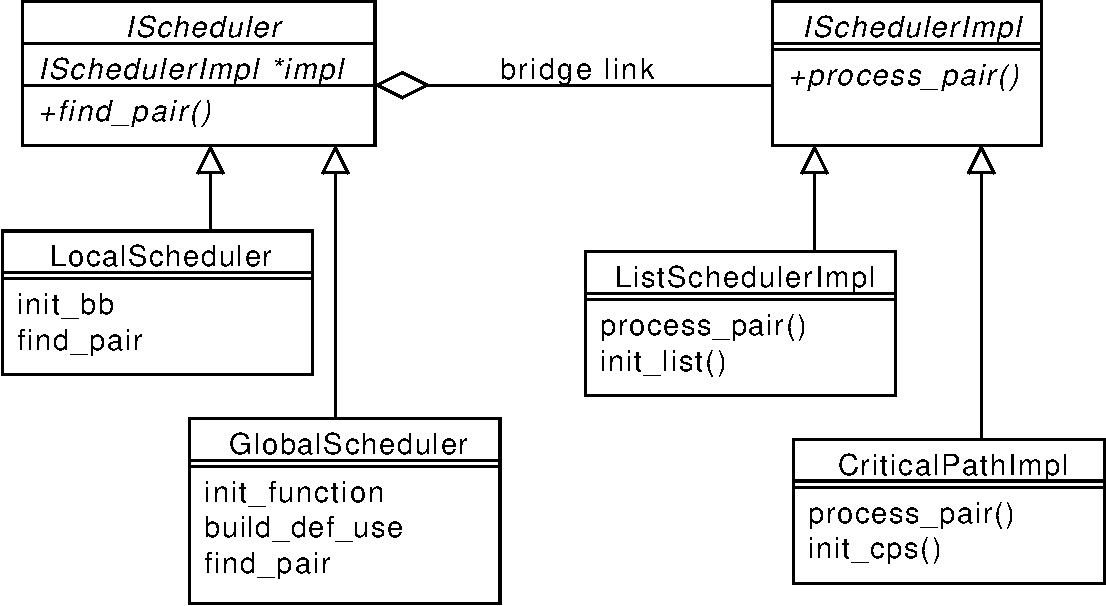
\includegraphics[width=0.8\textwidth]{illustrations/sched-bridge-crop.pdf}
\caption{Паттерн Bridge}
\label{fig:bridge_pattern}
\end{figure}

Благодаря абстрактному интерфейсу скрывающему реализацию, здесь также выполняется ISP.

\subsubsection{Паттерны поведения}

Паттерны поведения -- самый интересный раздел, среди них интересны почти все. Например при рассмотрении стандартной библиотеки, будет рассмотрено использование паттерна Итератор (для итераторов) и паттерна Стратегия (для аллокаторов). В качестве характерного примера поведенческих паттернов здесь можно рассмотреть паттерн Наблюдатель.

Этот паттерн позволяет как бы ``подписать'' один объект на уведомления другого. Пусть объект, который содержит данные будет простым и не содержит ничего кроме целого числа (и вектора наблюдателей).

\begin{lstlisting}
class Subject {
    vector < class Observer * > views; 
    int value;
  public:
    void attach(Observer *obs) {
        views.push_back(obs);
    }
    void setVal(int val) {
        value = val;
        notify();
    }
    int getVal() {
        return value;
    }
    void notify();
};
\end{lstlisting}

В функции \lstinline!notify! также нет ничего сложного: она просто уведомляет всех наблюдателей о смене состояния.

\begin{lstlisting}
void Subject::notify() {
  for (int i = 0; i < views.size(); i++)
    views[i]->update();
}
\end{lstlisting}

Теперь нужно договориться что наблюдают наблюдатели. Предположим, что частное или остаток от деления числа субъекта на заданное число (в реальных программах все будет сложнее, но это учебный пример).

Общий класс задает виртуальный метод \lstinline!update! для реализации в подклассах.

\begin{lstlisting}
class Observer {
    Subject *model;
    int denom;
  public:
    Observer(Subject *mod, int div) {
        model = mod;
        denom = div;
        model->attach(this);
    }
    virtual void update() = 0;
  protected:
    Subject *getSubject() {
        return model;
    }
    int getDivisor() {
        return denom;
    }
};
\end{lstlisting}

Теперь два подкласса.

\begin{lstlisting}
class DivObserver: public Observer {
  public:
    DivObserver(Subject *mod, int div): Observer(mod, div){}
    void update() {
        int v = getSubject()->getVal(), d = getDivisor();
        cout << v << " div " << d << " is " << v / d << '\n';
    }
};

class ModObserver: public Observer {
  public:
    ModObserver(Subject *mod, int div): Observer(mod, div){}
    void update() {
        int v = getSubject()->getVal(), d = getDivisor();
        cout << v << " mod " << d << " is " << v % d << '\n';
    }
};
\end{lstlisting}

Все это складывается вместе вот в такую замечательную городушку.

\begin{lstlisting}
int main() {
  Subject subj;
  DivObserver divObs1(&subj, 4);
  DivObserver divObs2(&subj, 3);
  ModObserver modObs3(&subj, 3);
  subj.setVal(14);
}
\end{lstlisting}

\textbf{Вопрос к студентам:} и что будет на экране?

\ifanswers
Правильный ответ: частное от деления 14 на 4 это 3, на 3 это 4 и в обоих случаях 2 в остатке. Так что 3, 4, 2.
\fi

\pagebreak
\subsection{Домашняя наработка по ООП}

\textbf{Контрольные вопросы}

\begin{enumerate}
\item Может ли нестатический метод в структуре вызывать статический метод?
\item Можно ли создать объект класса в конструкторе этого класса?
\item Можно ли создать объект класса в деструкторе этого класса?
\item Имеет ли смысл ключевое слово explicit для конструктора без аргументов?
\item Достаточно ли объявление класса для использования указателей на его методы?
\item Почему у конструкторов и деструкторов нет возвращаемых значений?
\item Можно ли перегрузить деструктор (так же как мы перегружаем конструкторы)?
\item Назовите оба способа задать неявное преобразование типов для вашего класса.
\item В лекциях рассмотрены const методы. Бывают ли volatile методы классов?
\item Может ли возникнуть необходимость объявить поле одновременно const и mutable?
\item Чем отличается указатель на статический метод от указателя на нестатический?
\item Что означает сокращение RAII, зачем нужна эта идиома?
\item Чем плоха идея реализовать копирующий конструктор через вызов оператора присваивания к *this?
\item Может ли быть скопирован по умолчанию объект класса с полем-ссылкой?
\item Что означает сокращение RVO, для чего используется?
\item Чем плоха идея перегрузить фигурные скобки (наравне с квадратными и круглыми)?
\item В лекциях рассматриваются операторы new и sizeof. Почему это операторы, а не функции?
\item Сохраняется ли правая ассоциативность при переопределении += или -=? Почему да или почему нет?
\item Возможно ли переопределить правый декремент для классов с запрещенным копированием?
\item Перечислите стандартные и пользовательские формы new и delete
\item В каких случаях деструктор нужно вызывать явно?
\item Можно ли вызвать (тем или иным способом) конструктор класса?
\item Как выбрать между правой и константной левой ссылкой?
\item Есть ли смысл в константных правых ссылках?
\item В лекциях рассмотрено связывание левой ссылки с правой (класс RefBind). Возможно ли связывание в обратном направлении?
\item Как выбрать между конструктором копирования и перемещения?
\item Зачем в языке и std::move и std::forward если оба это просто static cast?
\item За счет каких механизмов языка мы можем использовать универсальные ссылки?
\item Работает ли std::forward для идеального проброса правых ссылок?
\item Как привести указатель на объект производного класса к ссылке на объект базового?
\item Во сколько обычных вызовов по косвенности может обойтись вызов виртуальной функции?
\item Можно ли получить указатель на чисто виртуальную функцию?
\item В C++ нет статических деструкторов. Если бы они были, что мог бы делать виртуальный статический деструктор?
\item Может ли виртуальная функция быть статической? А чисто виртуальная?
\item Зачем нужны виртуальные деструкторы?
\item Может ли виртуальная функция быть объявлена inline?
\item Возможно ли корректно скопировать производный класс по указателю на базовый?
\item Что такое проблема срезки и как она проявляется?
\item Что обозначает аббревиатура NVI, зачем нужна эта идиома?
\item Могут ли в чисто виртуальных функциях быть аргументы по умолчанию?
\item В чем отличия композиции от закрытого наследования?
\item Чем отличается виртуальное наследование от невиртуального?
\item Имеют ли смысл виртyальные базовые классы при одиночном наследовании?
\item Почему виртуальное наследование отключает понижающий static cast по иерархии?
\item У вас есть выбор между использованием dynamic cast и typeid для проверки типа, в каком случае чем вы воспользуетесь?
\item Расшифруйте аббревиатуру SOLID и объясните кратко каждую из входящих в неё аббревиатур.
\item Что такое закон Деметры?
\item Выберите любой из классических паттернов проектирования и объясните его применимость.
\end{enumerate}

\textbf{Задания}

\begin{enumerate}
\item
Расширьте код игры в мяч до трёхмерной 

\item
Введите в код игры в мяч примитивы синхронизации чтобы его можно было запускать в многопоточном окружении

\item
Расширьте код до игры в мяч со смещающимся центром тяжести (допустим мяч наполовину заполнен водой или песком)

\item
Разработайте конкретный класс \lstinline!CTime!, предназначенный для хранения текущего времени и вычисления временных интервалов. Не ограничивайтесь unix time, сделайте возможным, например, подсчёт количества часов от Куликовской битвы до Бородинского сражения

\item
Как можно улучшить рассмотренный в (\ref{RAII}) класс CFile? Реализуйте и протестируйте обёртку.

\item
Разработайте и реализуйте иерархию классов, для управления сетевым соединением. Предусмотрите как минимум классы для TCP и UDP сокетов, наследующие от общего предка

\item
Реализуйте абстрактный интерфейс материальной точки и унаследуйте от него разные варианты мяча -- идеальный, с сопротивлением воздуха, со смещённым центром тяжести, etc. На основе общего интерфейса, реализуйте игрока в мяч, которому всё равно каким мячом играть

\item
Перегрузите для класса комплексных чисел, приведённых в (\ref{OperatorOverloading}) инкремент, логические операции, вычитание

\item
Разработайте класс кватернионов со всеми перегруженными арифметическими операциями. Исследуйте есть ли смысл наследовать его от комплексных чисел.

\item
Разработайте класс для операций над матрицами. Проиллюстрируйте к каким проблемам может привести ставшее некоммутативным умножение.

\item
Для вашего класса операций над матрицами перегрузите выделение и освобождение памяти. Разработайте стратегию выделения памяти для разреженных матриц. Проиллюстрируйте умножение двух разреженных матриц 10000x10000 в каждой из которых значимыми являются всего 2-3 элемента (остальные нули).

\end{enumerate}

\pagebreak
\section{Особая шаблонная магия}

Шаблоны, введённые в C++ были в своё время введены туда экспериментально. Их не было ни в одном другом языке и никто по настоящему не знал, что из этого получится. Поэтому большинство интересных и важных свойств шаблонов не были разработаны. Они были открыты. В этом разделе курса, вас тоже ожидают открытия.

Многие небезосновательно считают шаблонную подсистему языка C++ самой развитой и сложной в мире современного программирования (по крайней мере -- мейнстримного). Ещё интереснее взаимодействие этой подсистемы с объектно-ориентированными возможностями языка, а также потрясающие средства (такие как вариабельные шаблоны, кортежи и лямбда-выражения) которые становятся доступны для улучшения абстракций и порождения более компактного и быстрого кода. Но даже простые шаблоны функций, с которых и начинается изложение, таят в себе массу сюрпризов.

\subsection{Шаблоны функций\index{function template}}\label{FunctionTemplates}

Общий обзор шаблонных функций уже был проведен в (\ref{FunctionTemplate}), теперь настало время углубиться в детали и обсудить шаблонные функции в подробностях, прежде чем переходить к более сложным шаблонам классов.

\textbf{Вопрос к студентам:} как написать пару \lstinline!min! и \lstinline!max!?

\ifanswers
Правильный ответ: вариантов много, один из них см. ниже:
\fi

Возможный вариант ответа использует константные ссылки, но это могли бы быть и значения и правые ссылки.

\begin{lstlisting}
template <class T> const T&
max (const T &x, const T &y)
{
  return ((x > y) ? x : y);
}

template <class T> const T&
min (const T &x, const T &y)
{
  return ((x < y) ? x : y);
}
\end{lstlisting}

Классическим тестом на минимакс является переход 

$\forall x, y | x <= y \quad min(x,y) = x \wedge max(x, y) = y$

Обобщённые функции можно вызывать из обобщённых функций, так что тест тоже может быть шаблонным:

\begin{lstlisting}
template <typename T> bool
test_minmax (const T &x, const T &y)
{
  assert (x <= y);
  return (min<T> (x, y) == x) && (max<T> (x, y) == y);
}

\end{lstlisting}

В данном случае можно протестировать на паре чисел, паре символов, паре чисел с плавающей точкой, etc:

\begin{lstlisting}
assert(test_minmax<char> ('a', 'b'));
assert(test_minmax<int> (5, 6));
assert(test_minmax<double> (3.0, 7.2));
/* ... */
\end{lstlisting}

\subsubsection{Вывод типов шаблонами}\label{TemplateInference}

Если бы всегда при работе с шаблонами возникала необходимость явно указывать шаблонные аргументы, код довольно скоро разрастался бы, обрастая ненужными подробностями. Скажем так ли нужно писать \lstinline!test_minmax<int> (5, 6)! если компилятор достаточно умён, чтобы понять и более простую форму \lstinline!test_minmax(5, 6)! из контекста? Таким образом можно переписать:

\begin{lstlisting}
assert(test_minmax ('a', 'b'));
assert(test_minmax (5, 6));
assert(test_minmax (3.0, 7.2));
/* ... */
\end{lstlisting}

Положившись на аргументов шаблонными функциями. Он похож на вывод в \lstinline!auto! (\ref{DecltypeAuto}), но исторически он появился раньше и работает несколько слабее. Можно рассмотреть шаблонную функцию, принимающую указатель на некую функцию произвольного типа.

\begin{lstlisting}
template <typename Func> Func 
deduce(const Func & f)
\end{lstlisting}

Здесь для \lstinline!void f() {}! выведенным типом при вызове \lstinline!deduce(f)! будет \lstinline!void(*)()!. Но что если нужно вывести не тип указателя на функцию, а возвращаемый тип функции? Увы, с классическими шаблонами это сделать нелегко: тип выводится из типа аргумента и только. 

\textbf{Вопрос к студентам:} какие новые возможности даёт здесь использование \lstinline!decltype!?

\ifanswers
Правильный ответ: способ довольно очевиден.

\begin{lstlisting}
template <typename Func>
auto deduce(const Func & f) -> decltype(f())
\end{lstlisting}

В данном случае типом возвращаемого значения для \lstinline!deduce(f)! будет \lstinline!void!
\fi 

При выводе типов шаблоны сворачивают ссылки (левые и правые) так же, как это делает \lstinline!auto!.

\begin{lstlisting}
template <typename T>
void foo(T&& t);
\end{lstlisting}

Пусть теперь \lstinline!foo! вызвана с аргументом \lstinline!x! типа \lstinline!X!, причём \lstinline!x! является lvalue. Тогда \lstinline!T! разрешается в \lstinline!X&!, а реальным типом аргумента t будет \lstinline!X& &&!, то есть \lstinline!X&!. Если же \lstinline!x! является rvalue, то \lstinline!T! разрешается в \lstinline!X! и реальным типом аргумента \lstinline!t! будет \lstinline!X&&!.

В некоторых случаях, вывод не работает -- например не выводится тип возвращаемого значения:

\begin{lstlisting}
// SrcT can be deduced, but DstT cannot 
template <typename DstT, typename SrcT> 
inline DstT implicit_cast (SrcT const& x)  
{ 
    return x; 
} 
\end{lstlisting}

Здесь этот тип необходимо указывать явно.

\begin{lstlisting}
double value = implicit_cast<double>(-1); 
\end{lstlisting}

При этом второй тип легко выводится из типа аргумента и его можно не указывать.

\subsubsection{Обобщенность и неожиданности}\label{GenericCode}

Пока что с функциями \lstinline!max! и \lstinline!min! всё было хорошо -- все три теста проходят, в чем несложно убедиться. Но обобщённые функции могут принимать переменные любого рода. Пусть имеется очень простая структура, определяющая имя и возраст человека

\begin{lstlisting}
struct Person
{
  const char *name;
  int age;
  Person (const char *a_name, int an_age) : 
      name (a_name), age(an_age) {}
};

bool
operator > (const Person &lhs, const Person &rhs)
{
  return lhs.age > rhs.age;
}

bool
operator < (const Person &lhs, const Person &rhs)
{
  return lhs.age < rhs.age;
}

bool
operator <= (const Person &lhs, const Person &rhs)
{
  return !(lhs > rhs);
}

bool
operator == (const Person &lhs, const Person &rhs)
{
  return (&lhs == &rhs);
}
\end{lstlisting}

И вот появляются Иван и Данила:

\begin{lstlisting}
Person Ivan ("Ivan", 24);
Person Danila ("Danila", 24);
std::printf ("%d\n", test_minmax (5, 6));
std::printf ("%d\n", test_minmax (Ivan, Danila));
\end{lstlisting}

\textbf{Вопрос к студентам:} что будет на экране?

\ifanswers
Неожиданно на экране будет 1 и 0. Такое поведение функций, когда для пары одинаковых объектов они сохраняют их значения и порядок в результирующей паре, называется стабильностью. Можно сделать вывод, что функции \lstinline!min! и \lstinline!max! ведут себя \textbf{нестабильно}. Проблемы стабильности также возникают при проектировании обобщённых алгоритмов сортировки, бинарного поиска и многих других.
\fi

\textbf{Вопрос к студентам:} как переопределить нашу пару функций так, чтобы они стали стабильными?

\ifanswers
Один из вариантов решения

\begin{lstlisting}
template <class T> const T&
max (const T &x, const T &y)
{
  return ((x > y) ? x : y);
}

template <class T> const T&
min (const T &x, const T &y)
{
  return ((x <= y) ? x : y);
}
\end{lstlisting}
\fi

Какая мораль? Разработка обобщенного кода очень сильно отличается от разработки конкретного кода. Нужно серьёзно вникать в детали, которых может вовсе не возникнуть когда вы работаете с заранее определенными данными. Все дальнейшие лекции будут посвящены обобщенному коду: шаблонной магии, параллельным алгоритмам и контейнерам стандартной библиотеки, исключениям. 

\textbf{Домашняя наработка:} Для трёх элементов, можно написать три порядковых статистики -- максимум, медиану и минимум. Попробуйте написать их в терминах уже написанных бинарных \lstinline!min! и \lstinline!max!, предполагая, что бинарные \lstinline!min! и \lstinline!max! стабильны. Сможете ли вы сделать тернарные варианты также стабильными?

\subsubsection{Перегрузка шаблонных функций}\label{TemplOverloading}

Правила перегрузки шаблонных функций являются расширением правил перегрузки обычных функций, рассматривавшихся ранее в (см. \ref{Overloading}), но со спецификой обобщённого кода. Простые случаи действительно просты. 

\begin{lstlisting}
/* 1. max of two ints */
inline int const& max (int const& a, int const& b)
{
  return a < b ? b : a;
}

/* 2. maximum of two values of any type */
template <typename T>
inline T const& max (T const& a, T const& b)
{
  return a < b ? b : a;
}
\end{lstlisting}

Немного тренировки:

\begin{lstlisting}
  max(7, 42);         /* calls [1]         */
  max(7.0, 42.0);     /* calls [2]<double> */
  max<int>(7, 42);    /* calls [2]<int>    */
  max<>(7, 42);       /* calls [2]<int>    */
  max('a', 42.7);     /* calls [1]         */
\end{lstlisting}

Последний пример показывает, что в рассмотренной ранее (см. \ref{Overloading}) лестнице разрешения перегрузок, шаблоны добавляют один дополнительный шаг: после проверки совершенного совпадения, компилятор проверяет шаблоны, после чего возвращается к возможности применения преобразований и неточного совпадения.

Это объясняет проблему с перегрузкой по универсальной ссылке (см. \ref{UniversalReferences}). При разрешении универсальной ссылки как в правую, так и в левую, получившаяся конструкция становится perfect match, что и эксплуатирует второй добавленный шаг.

Однако в обобщённом коде, обобщённые типы можно уточнять квалификаторами. В этом случае общее правило состоит в том, что более специальный вариант всегда выигрывает у менее специального.

\begin{lstlisting}
template <typename T> void f(T*); // (1)
template <typename T> void f(T**); // (2)

int ****a;
f(a); // calls (2)
\end{lstlisting}

Второй вариант более специален, поэтому там, где он может быть использован, он выигрывает у первого.

Можно потренировать интуицию. Есть три кандидата на вызов.

\begin{lstlisting}
template <typename T1, typename T2> void f( T1, T2 ); /* (1) */
template <typename T> void f( T, T* ); /* (2) */
template <typename T> void f( double, double* ); /* (3) */
\end{lstlisting}

И вызов функции, который подходит под все эти шаблоны:

\begin{lstlisting}
double t, s;
f (t, &s);
\end{lstlisting}

\textbf{Вопрос к студентам:} какая функция будет вызвана?

\ifanswers
Все три варианта являются perfect match, но один из них является наиболее частным, один более общим и один максимально общим. В таких случаях компилятор всегда выбирает наименее общий вариант: то есть сначала (3), если  его вычеркнуть, то (2) и в последнюю очередь (1). Но с этим правилом надо быть осторожным, поскольку оно работает только когда и впрямь есть семантически точное совпадение. В другом примере:

\begin{lstlisting}
template <typename T> void f( T, T ); /* (1) */
template <typename T> void f( double*, T* ); /* (2) */
template <typename T> void f( T*, double* ); /* (3) */
template <typename T1 typename T2> void f( T1*, T2 ); /* (4) */
template <typename T1 typename T2> void f( T1, T2* ); /* (5) */
template <typename T1 typename T2> void f( T1*, T2* ); /* (6) */
\end{lstlisting}

При вызове функции:

\begin{lstlisting}
double t, s;
f (&t, &s);
\end{lstlisting}

Точное совпадение даётся всеми перечисленными функциями, при этом важность того, что типы равны (случай 1) не перевешивает важность того, что оба эти типа указатели (случай 6). В итоге компилятор не может придти к решению и выдаст ошибку ``is ambiguous''. Если вычеркнуть (1, 2, 3), то оставшиеся разрешатся в пользу (6) как наиболее общего совпадения. Но (и это интересно), если оставить (1, 4 и 5), то это всё ещё будет ошибка. Зато (2, 4, 5) однозначно разрешаются в пользу (2). Но оба выигравших номера -- 2 и 6 дают ошибку в паре с 1. Мораль у этого такая: всегда нужно смотреть на наиболее общий семантический тип.
\fi

\textbf{Домашняя наработка:} рассмотрите случай, когда одновременно объявлены одновременно шаблоны для ссылки и константной ссылки

\begin{lstlisting}
template <typename T> inline T& 
max (T& a, T& b) { /* ... */ }

template <typename T> inline T const& 
max (T const& a, T const& b) { /* ... */ }
\end{lstlisting}

Как в этом случае будет разрешаться перегрузка? Приведите примеры. Аналогично для указателя, константного указателя, указателя на константные данные. Если добавить к перегрузке по ссылке перегрузку по значению, создав тем самым неоднозначность, компилятор должен отреагировать ошибкой. Проверьте как отработает эту ситуацию ваш компилятор.

\subsubsection{Управление инстанцированием шаблонов функций}\label{InstancingFuncs}

Пусть задана довольно простая шаблонная функция с довольно простым использованием -- возведение в квадрат чисел разных типов.

\begin{lstlisting}
template<class T>
T square(T n)
{
  return n * n;
}

int
main ()
{
  int x = square (3);
  float y = square (3.0);
  return 0;
}
\end{lstlisting}

\textbf{Вопрос к студентам:} сколько копий этой функции будет в объектном файле и какие они будут?

\ifanswers
В вопросе конечно есть подвох:

\begin{verbatim}
$ g++ -c square.cc
$ objdump -tC square.o
\end{verbatim}

даёт 

\begin{verbatim}
_Z6squareIiET_S0_
_Z6squareIdET_S0_ 
\end{verbatim}

Что соответствует:

\begin{lstlisting}
int square<int>(int);
double square<double>(double);
\end{lstlisting}
\fi

Вопрос мотивирует какие-то способы исследования реального результата работы компилятора в области подстановки шаблонов. Приведенный в ответе вызов

\begin{verbatim}
$ objdump -tC square.o
\end{verbatim}

Это Linux-специфичный способ посмотреть таблицу символов объектного файла.

Но что будет если функция оказалась сразу в двух единицах трансляции?

\begin{lstlisting}
#ifndef MAX_GUARD_
#define MAX_GUARD_

template <typename T> T
max (T x, T y)
{
  return (x > y) ? x : y;
}

extern int foo (int x, int y);
extern int bar (int x, int y);

#endif
\end{lstlisting}

и в обоих функциях \lstinline!foo! и \lstinline!bar!, находящихся в модулях maxuser1.cc и maxuser2.cc происходит вызов \lstinline!max(x, y)!?

\begin{verbatim}
$ g++ maxuser1.cc -c
$ objdump -tC maxuser1.o
  w    F .text._Z3maxIiET_S0_S0_

$ g++ maxuser2.cc -c
$ objdump -tC maxuser2.o
  w    F .text._Z3maxIiET_S0_S0_
\end{verbatim}

Видно, что теперь функция с одинаковым именем есть в обоих модулях.

\textbf{Вопрос к студентам:} почему это не нарушение ODR?

\ifanswers
Верный ответ: в ODR для шаблонных функций слово one означает один на модуль
\fi

Итак, их все ещё можно слинковать вместе и линкер произвольно выберет одну из них (благо обе идентичны).

Увы, если из этих модулей нужно собрать библиотеку:

\begin{verbatim}
ar cruv libmax.a maxuser1.o maxuser2.o
objdump -tC libmax.a
\end{verbatim}

то в этой библиотеке окажется две копии функции. Хуже того: при компиляции каждого модуля эта функция должна быть N раз независимо построена и соптимизирована. Очень плохо. Ещё хуже если некий модуль собирался с одними опциями оптимизации, а другой с другими.

Можно заблокировать инстанцирование, поместив в один из модулей (например в maxuser2.cc) явное указание, что шаблон уже был инстанцирован с этими параметрами где-то ещё:

\begin{lstlisting}
extern template int max<int> (int, int);
\end{lstlisting}

Теперь лишний раз функция инстанцирована не будет:

\begin{verbatim}
$ g++ --std=c++14 maxuser2.cc -c
$ objdump -tC maxuser2.o
g     F .text	0000000000000024 bar(int, int)
         *UND*	0000000000000000 int max<int>(int, int)
g     F .text	0000000000000038 main
         *UND*	0000000000000000 foo(int, int)
\end{verbatim}

Но конечно неясно что такого особенного в модуле maxuser2. Для того чтобы решить эту проблему в более общем виде, можно заблокировать инстанцирование с этим типом везде кроме принудительной точки инстанцирования:

В max.hpp:

\begin{lstlisting}
extern template int max<int> (int, int);
\end{lstlisting}

И в новом модуле max.cc

\begin{lstlisting}
#include "max.hpp"
template int max<int>(int, int);
\end{lstlisting}

Эта техника, введенная в C++14 позволяет гибко управлять точками инстанцирования, блокируя или вынуждая компилятор инстанцировать те или иные шаблоны. Здесь речь о шаблонах функций, исследование шаблонов классов -- более тонкое искусство (см. \ref{ControlInstancing}).

\subsection{Два полиморфизма\index{Template Polymorphism}}\label{TemplatePolymorphism}

Что же, к этому моменту вы знаете о шаблонах функций уже достаточно, чтобы вернуться к серьёзным вещам, таким как планеты и космические корабли. Можно наследовать их от общего предка, как это делалось в (\ref{PureVirtual}), но совершенно не задействовать виртуальные функции:

\begin{lstlisting}
class CelestialBody
{
  double x, y;
public:
  double get_x () const;
  double get_y () const;
  /* ... other ... */ 
};

class SpaceShip : public CelestialBody
{
  /* ... spaceship-related ... */
};

class Planet : public CelestialBody
{
  /* ... planet-related ... */
};
\end{lstlisting}

И тем не менее сохранить возможность писать довольно абстрактный код, полагающийся только на общий интерфейс объектов (способность сообщить координаты) и отдающий им на откуп детали реализации:

\begin{lstlisting}
template <typename T> double
get_distance (const T &lhs, const T & rhs)
{
  double xdist = lhs.get_x() - rhs.get_x();
  double ydist = lhs.get_y() - rhs.get_y();
  return sqrt (xdist*xdist + ydist*ydist);
}
\end{lstlisting}

Это прекрасное свойство называется полиморфизм времени компиляции, или статический полиморфизм. Заметьте, никаких больше виртуальных функций, никаких таблиц виртуальных методов, никакого оверхеда времени выполнения (за счёт раздутия кода помещением туда 100500 экземпляров функции \lstinline!get_distance!, разумеется).

Разница в том, что класс \lstinline!ICelestialBody! создавал явный интерфейс, в случае же статического полиморфизма, шаблонная функция накладывает неявные требования к обоим своим инстанциирующим типам, сформулированные точно так же ``поддерживать функцию-член \lstinline!get_x()!'' и ``поддерживать функцию-член \lstinline!get_y()!''. 

При рассмотрении нового стандарта будут рассмотрены ``концепты'', которые наконец-то определяют способ задать неявный интерфейс явно, см. (\ref{Concepts}).

Ещё более важным примером полезности шаблонного полиморфизма является его ``утиная'' сущность (если нечто плавает как утка и крякает как утка, то это утка). Например, функторы \textbf{не являются} взаимозаменяемыми с указателями на функции. Если некая функция ждёт указатель, передать ей функтор даже с той же сигнатурой -- нельзя. 

Для примера:

\begin{lstlisting}
struct Pred 
{
  int operator()(int x);
};
\end{lstlisting}

Этот функтор нельзя использовать с явным интерфейсом:

\begin{lstlisting}
int filtered_sum(int numbers[], int len, int (*pred)(int))
{
  int i, a = 0;

  for (i = 0; i != len; ++i)
    if (pred(numbers[i]) { a += numbers[i]; }

  return a;
}

Pred p;
filtered_sum (nums, 10, p); // error;
\end{lstlisting}

К счастью, при работе с неявными шаблонными интерфейсами, требование к типу быть выполнимым-как-функция позволяет прозрачно передавать и функторы и указатели на функции в качестве такого типа.
 
\begin{lstlisting}
template <typename FuncType>
int filtered_sum (int numbers[], 
                  int len, FuncType pred) 
{ 
  /* ... same body ... */ 
}

Pred p;
filtered_sum (nums, 10, p); // ok;
\end{lstlisting}

\textbf{Вопрос к студентам:} что будет при попытке вызвать функцию \lstinline!max! передав в качестве аргумента \lstinline!std::complex!?

\ifanswers
Правильный ответ: увы, на комплексных числах нельзя ввести ни порядка ни даже частичного порядка. Будет ошибка компиляции.
\fi

\subsubsection{Когда C++ быстрее, чем C}\label{CppBetterC}

Благодаря статическому полиморфизму, даже простые шаблоны функций не так просты и их не стоит недооценивать. 

\textbf{Вопрос к студентам:} какую сигнатуру вы напишете, если хотите на C написать обобщённую функцию сортировки? 

\ifanswers
Ответ: стандарт языка C99 регламентирует (пункт 7.20.5.2) следующую сигнатуру:

\begin{lstlisting}
void qsort (void *base, size_t nmemb, size_t size, 
            int (*compar)(const void *, const void *));
\end{lstlisting}
\fi

Почему в этой сигнатуре использован \lstinline!void*!? Потому что в обобщённой функции не известно какого типа элементы будут отсортированы. Кроме того требуется передавать размер элемента и их количество раздельно, что открывает возможности для человеческих ошибок. Но хуже всего то, что компаратор (вызываемый на каждое сравнение элементов) это указатель на функцию. Из-за этого:

\begin{itemize}
\item Каждый вызов компаратора имеет штраф на разыменование указателя на функцию -- лишний уровень косвенности
\item Исключена возможность inline-подстановки сравнения, которое обычно сводится к чему-то очень простому (скажем простому ``меньше, чем'')
\end{itemize}

Всех этих недостатков лишена реализация в стиле C++, которая может выглядеть примерно как:

\begin{lstlisting}
/* we suppose that Element class have 
   operator< () redefinition */
template <typename Element>
void qsortpp (Element *base, size_t nmemb);
\end{lstlisting}

Это лучше, проще, более безопасно относительно типов и это гораздо эффективнее. Платой за это является объём кода, который компилятор теперь сгенерирует для каждой инстанциации \lstinline!qsort!, но это недорого.

На самом деле стандарт C++98 регламентирует (C++98 25.3.1.1) даже более изящную сигнатуру для стандартной сортировки:

\begin{lstlisting}
template <class RandomAccessIterator>
void sort (RandomAccessIterator first, 
           RandomAccessIterator last);
\end{lstlisting}

Но вся её мощь, красота и обобщённость проявятся позже, когда речь пойдёт о стандартной библиотеке.

\textbf{Вопрос к студентам:} что принципиально мешает ввести шаблоны в язык C (даже не вводя туда классы, просто шаблоны функций)?

\ifanswers
В этом случае не обойтись без манглирования имён, чего в случае C никто не хочет
\fi

\textbf{Домашняя наработка:} Реализуйте \lstinline!qsort! в стиле C и в стиле C++

\subsubsection{Когда шаблонный полиморфизм уступает динамическому}\label{DynamicBetterStatic}

Использование шаблонного полиморфизма снижает накладные расходы на исполнение и почти всегда предпочтительно. Но есть вещи, которые требуют динамического полиморфизма и оказываются неоправданно сложными если пытаться сделать их на этапе компиляции.

\begin{lstlisting}
class obj
{
public:
  virtual int foo (int) = 0;    
};

class A : public obj;
class B : public obj;

/* ... class C, D, etc ... */

/* returns A is config have 'a', B is 'b', and so on ... */
obj * getfromconfig (const char *filename);

int
entry (obj *x)
{
  return x->foo();
}

int
main (void)
{
  return entry (getfromconfig("my.xml"))
}
\end{lstlisting}

Этот код представляет собой идиому ``виртуального конструктора'' (так же известен как фабричный метод).

\textbf{Домашняя наработка:} попробуйте переписать его с использованием только статического полиморфизма.

\pagebreak
\subsection{Шаблоны классов\index{class template} и специализация}\label{ClassTemplates}

Допустим, стоит задача спроектировать стек – класс объектов любого типа (но однородных) которые будут туда помещаться и вытаскиваться. Как обычно синтаксис вполне понятен через пример (детали всегда можно прочитать в стандарте).

\lstinputlisting[firstline=6,lastline=18]{cpp_code/p3s2.cpp}

Обратите внимание на то, что \lstinline!T!, помещённый в шаблон, используется внутри класса как совершенно обычный тип. Можно вернуть его из метода, передать в метод и даже использовать как деталь реализации скрытой подструктуры.

\lstinputlisting[firstline=20,lastline=37]{cpp_code/p3s2.cpp}

\textbf{Вопрос к студентам:} чего здесь явно не хватает?

\ifanswers
Ожидается хоровой ответ: деструктор, копирующий конструктор и оператор присваивания. Позвать кого-нибудь к доске разобрать как их писать.
\fi

Давайте посмотрим как применять разработанный шаблонный класс:

\lstinputlisting[firstline=39]{cpp_code/p3s2.cpp}

Из примера ясно, что с использованием шаблонов, поддержка двух разнородных контейнеров (трёх, десяти) это крайне легко. Скорость компиляции, правда, страдает, вместе с объёмом кода, но по современным реалиям это невысокая цена.

\subsubsection{Специализация\index{template specialization}}\label{TemplateSpec}

В случае с функциями был использован механизм перегрузки функций чтобы получить специальное поведение для конкретного типа аргументов. Но нельзя ``перегрузить'' класс. Зато вы можете специализировать шаблон класса для конкретных шаблонных параметров. Синтаксис, опять же, прост:

\begin{lstlisting}
template <>
class Stack<int> { ... };
\end{lstlisting}

Такая запись создаёт отдельное поведение для стеков, параметризованных целыми числами. Реализация и поведение такого шаблона могут не иметь вообще ничего общего с исходным. Это создаёт почти такую же радость при чтении кода на C++ как перегрузка операторов и неявные приведения.

Важным является тот факт, что специализация всегда должна физически в коде следовать общему шаблону (The declaration of a specialization must always follow the declaration of the template which is being specialized (14.7.3/3)) и поэтому нельзя сначала написать специализированную версию, а потом общую -- общая версия долна быть хотя бы \textbf{объявлена} раньше.

Функции тоже могут быть специализированы (как и перегружены), что создаёт известную ортогональность. По правилам C++ вторая перегрузка выигрывает у первой, а потом специализация выигрывает у оригинала:

\begin{lstlisting}
template <typename T> void foo(T);
template <typename T> void foo(T*); 

// specialization of both foo(T) and foo(T*)
template <> void foo<int>(int*); 

foo(new int); // calls foo<int>(int*);
\end{lstlisting}

Но тут важно, что компилятор засчитывает специализацию для типов, уже встретившихся ему внутри единицы трансляции. Поэтому (это известно как ``контрпример Димова-Абрамса''):

\begin{lstlisting}
template <typename T> void foo(T);
// specialization of foo(T)
template <> void foo<int*>(int*); 
template <typename T> void foo(T*);

foo(new int); // calls foo(T*) !!!
\end{lstlisting}

В этом примере вторая перегрузка выигрывает у первой, после чего специализация вообще не рассматривается.

Стоп, скажете вы, как же так может быть, что явно более специальная версия функции с подходящими по типу аргументами оказывается выброшенной? Очень просто: специализации не участвуют в перегрузке. Комитет по стандартизации официально решил, что смена лидера перегрузки после специализации шаблона будет вводить программистов в заблуждение (недоуменное молчание, затем -- общий смех). На самом деле ничего смешного тут нет, это решение крайне логично, просто, чтобы понять эту логику, нужно понимать как инстанцируются шаблоны, в частности знать о SFINAE см. (\ref{SFINAE}).

Конечно вы не хотите таких эффектов в своей программе, поэтому там где можно перегрузить функцию, можно и нужно её перегружать, а не специализировать.

\textbf{Вопрос к студентам:} Бывают ли случаи когда необходимо все-таки специализировать функцию?

\ifanswers
Правильный ответ следует из предыдущего параграфа: это как раз те случаи, когда её \textbf{нельзя} перегрузить. Например стандарт регламентирует, что перегрузка функций из пространства имен \lstinline!std! запрещена, но часто хочется \lstinline!std::swap! для своих типов, в этом случае специализация -- единственный выход.
\fi

\subsubsection{Частичная специализация\index{partial specialization}}\label{PartialSpec}

Суть частичной специализации в том, что вы пишете отдельный код для случая когда только часть параметров исходного шаблона зафиксирована в некоторых значениях (или ограниченая некоторыми условиями). При исходном шаблоне

\begin{lstlisting}
template <typename T, typename U> class MyClass { ... };
\end{lstlisting}

Возможно написать, например, такие специализации

\begin{lstlisting}
/* partial specialization: T = U */ 
template <typename T> class MyClass<T,T> { ... }; 
/* partial specialization: U = int */ 
class MyClass<T,int> { ... }; 
/* partial specialization: T = T1*, U = T2* */
template <typename T1, typename T2> 
class MyClass<T1*,T2*> { ... };
\end{lstlisting}

И далее при подстановке конкретных типов будет инстанцирована та или иная специализация.

\begin{lstlisting}
MyClass<int,float> mif;   /* uses MyClass<T1,T2> */ 
MyClass<float,float> mff; /* uses MyClass<T,T> */ 
MyClass<float,int> mfi;   /* uses MyClass<T,int> */ 
MyClass<int*,float*> mp;  /* uses MyClass<T1*,T2*> */
\end{lstlisting}

Учтите, что если под некое объявление подходят сразу два варианта частичной специализации, то это ошибка

\begin{lstlisting}
MyClass<int,int> m;   // ERROR: matches MyClass<T,T> 
                      //        and MyClass<T,int> 
MyClass<int*,int*> m; // ERROR: matches MyClass<T,T> 
                      //        and MyClass<T1*,T2*>
\end{lstlisting}

Можно исправить ошибку сделав уникально подходящий шаблон

\begin{lstlisting}
template <typename T> 
class MyClass<T*,T*> { ... };
\end{lstlisting}

Очень важно понимать, что частичная специализация не доступна для функций и является прерогативой шаблонов классов.

Саттер в известной публикации \url{http://www.gotw.ca/publications/mill17.htm} предлагает способ разрешить нечто вроде частичной специализации для функций:

\begin{lstlisting}
template<class T> 
struct FImpl;

template<class T> 
void f( T t ) { FImpl<T>::f( t ); } 

template<class T> 
struct FImpl 
{ 
  static void f( T t ); 
};
\end{lstlisting}

Частичная специализация в этом случае очевидно доступна для класса \lstinline!FImpl! и напрямую влияет на зависимый тип статической функции-члена.

Но в большинстве случае аналог частичной специализации для функций достигается перегрузкой.

\textbf{Дискуссия в аудитории:} Вы -- член комитета стандартизации и решаете сделать ли частичную специализацию доступной для функций. Ваши аргументы за и против?

\subsubsection{Вывод типов против подстановки типов}

Ранее (см. \ref{UniversalReferences}) уже обсуждались возможности автоматического вывода типов, в частности для организации универсальных ссылок:

\begin{lstlisting}
int x;
auto &&y = x;
\end{lstlisting}

\textbf{Вопрос к студентам:} вспомнить механизм вывода типов. Какой тип будет выведен для \lstinline!y!?

\ifanswers
Правильный ответ -- \lstinline!int&! так как для \lstinline!x! будет выведен тип \lstinline!int&!, а потом сработает свертывание ссылок.
\fi

Подобные техники возможны и для шаблонов:

\textbf{Вопрос к студентам:} в коде ниже аргумент \lstinline!push_back! это правая или универсальная ссылка?

\begin{lstlisting}
template <typename T, class Allocator = allocator<T>>
class Stack
{
  /* ... */
  public:
  void push_back(T&& x);
};

/* ... */
int x;
Stack <int> s;
s.push_back (x);
\end{lstlisting}

\ifanswers
Правильный ответ -- правая, так как вывод \lstinline!T! для вектора подставляется, а не выводится. Таким образом будет ошибка компиляции.
\fi

Но очень важно отличать механическую \textbf{подстановку} типа в шаблонах от гораздо более сложного \textbf{вывода} типов (который бывает в тех же шаблонах, например шаблонная функция вполне способна вывести тип аргумента без явного указания.

\subsubsection{Разрешение имён}

Шаблоны имеют дело с именами -- заменой имени для типа, выводом имени, разрешением имени. Очень сложные и очень тонкие баги связаны с разрешением имен шаблонами и почти все эти баги основываются на том, что программист не видит тонкого различия между зависимым и независимым именем.

Зависимое имя -- это имя, которое семантически зависит от шаблонного параметра. Шаблонный параметр может быть его типом, он может участвовать в формировании типа и так далее.

Золотыми буквами в памяти надо выбить фразу: \textbf{Разрешение зависимых имен откладывается до подстановки шаблонного параметра}.

Потренируемся:

\begin{lstlisting}
// template for foo
template<typename T> void 
foo (T) 
{ 
  cout << "T"; 
}

struct S { };

// t is dependent from T, s -- not
template<typename T> void 
call_foo (T t) 
{
  S x;
  foo (x);
  foo (t); 
}

// non-template overload
void 
foo (S) 
{   
  cout << "S"; 
}

int 
main () 
{
  S x; 
  call_foo (x); 
}
\end{lstlisting}

\textbf{Вопрос к студентам:} что на экране?

\ifanswers
Правильный ответ: TS. 

Более специальная функция \lstinline!foo! просто ещё не объявлена в точке вызова \lstinline!foo(x)!, а вот разрешение вызова \lstinline!foo(t)! откладывается до подстановки \lstinline!t!, которая происходит после объявления более специальной функции.
\fi

Полезный пример из \cite{vandervoord} даёт обратную картину: здесь \lstinline!Base::exit! ещё не существует, а имя функции \lstinline!exit! независимо от шаблонного параметра, поэтому оно ``схватит'' первую попавшуюся, скорее всего глобальную функцию \lstinline!exit!.

\begin{lstlisting}
template <typename T> 
class Base { 
  public: 
    void exit(); 
};

template <typename T> 
class Derived : Base<T> 
{ 
public: 
  void foo() 
  { 
    // calls external exit() or error! 
    exit();   
  } 
}; 
\end{lstlisting}

\textbf{Вопрос студентам:} что же делать.

\ifanswers
Правильный ответ: сделать \lstinline!exit! зависимым именем, например явно употребив \lstinline!Base::exit()!
\fi

Итак, я надеюсь, теперь все стало понятнее. Если нет, то вам не повезло.

В последнем примере говорилось про \lstinline!Base::exit!, а не про \lstinline!Base<T>::exit!, потому что для удобного оперирования именами в специализациях и шаблонах разрешено их сокращенное употребление:

\begin{lstlisting}
template <class T> class A {
  A* a1; // A refers to A<T>
};

template <class T> class A<T*> {
  A* a2; // A refers to A<T*>.
};
\end{lstlisting}

К счастью, классы нельзя перегружать, иначе все вообще бы запуталось.

\subsubsection{Исследование инстанцирования шаблонов классов}\label{ControlInstancing}

TODO: на примере Stack

\pagebreak
\subsection{Шаблоны и ООП}\label{OOTemplates}

Самые коварные места в языке -- это места сочленения различных его подсистем. Большинство языков программирования не являются мультипарадигменными и лишены этих проблем, но C++ это большой сложившийся конгломерат самых разных техник. На стыках этих техник часто возникают ситуации конфликта и взаимодействия. Особенно это касается использования возможностей ООП с учетом особенностей шаблонных классов. Как шаблоны соотносятся с наследованием, полиморфизмом, инкапсуляцией? Это неочевидно. Особенно интересна техника CRTP, когда шаблонный параметр причудливо переплетается с иерархией классов. Обо всем этом пойдет речь в этой лекции.

\subsubsection{Специализация методов класса}\label{MemberSpec}

Следующий пример вводит два класса: \lstinline!Data! это не шаблоннный класс с шаблонным методом \lstinline!read<T>! и \lstinline!DataReader<T>! это шаблонный класс с шаблонным методом \lstinline!read<R>!

\begin{lstlisting}
class Data {
public:
  template <typename T> T read() const;
};

template <typename T>  
class DataReader {
  const T& source_;
public:
  DataReader(const T& s) : source_ (s) {}
  /* internally calls source_.read() */
  template <typename R> R read();
};
\end{lstlisting}

Можно написать реализацию метода \lstinline!DataReader<T>::read<R>! вне тела класса, это довольно простое упражнение:

\begin{lstlisting}
template <typename T>
  template <typename R> 
R DataReader<T>::read()
{
  R foo = source_.read<R>();
}
\end{lstlisting}

На самом деле это не лучший вариант, потому что оставляет неолднозначность в синтаксисе. Её лучше сразу разрешить:

\begin{lstlisting}
R foo = source_.template read<R>();
\end{lstlisting}

Гораздо сложнее написать специализацию этого метода. Сложно даже поставить задачу. Например задача написать специализацию \lstinline!DataReader<T>::read<string>! сразу поставлена некорректно. Нужно запомнить, что написать специализацию метода можно только если полностью специализирован также его класс (иначе это было бы эквивалентно частичной специализации функций а она запрещена). Поэтому корректная задача это написать например \lstinline!DataReader<Data>::read<string>!. Она уже может быть решена:

\begin{lstlisting}
template <> template <> std::string 
DataReader<Data>::read() const
{
  std::string foo = "";
  return foo;
}
\end{lstlisting}

Немного вычурная конструкция \lstinline!template <> template <>! при этом обязательна.

\subsubsection{Переходники типов}\label{TypeToTypes}

Иногда не хочется писать специализацию или частичную специализацию всего класса ради того, чтобы изменить поведение одного нешаблонного метода. Если метод можно перегрузить, все хорошо. Но что если метод требует специализации (например у него просто нет аргументов подходящего для перегрузки типа)? 

Задача: пусть один и тот же метод \lstinline!func! класса \lstinline!<T1, T2> class A! должен по разному себя вести если \lstinline!T1! это целое число и если нет.

\begin{lstlisting}
A <int, double> a;
A <float, double> b;

a.func(); /* for int */
b.func(); /* forall */
a.bar(); /* forall */
b.bar(); /* forall */
\end{lstlisting}

\textbf{Вопрос к студентам:} как этого добиться?

\ifanswers
См. верный ответ ниже (разумеется предполагается немного подумать самому).
\fi

Первый вариант ответа может быть примерно такой:

\begin{lstlisting}
template <typename T1, typename T2>
class A
{
public:
  void func(void) { 
    T1 dummy; internal_func (dummy); 
  }
private:
  template< class V >
  void internal_func (V) { printf ("forall\n"); }

  void internal_func (int) { printf ("forint\n"); }
};
\end{lstlisting}

Но тут есть проблема -- заранее неизвестно, что именно делает конструктор объекта класса \lstinline!T1!. Стандартный выход из ситуации -- подход с использованием переходника: 

\begin{lstlisting}
template <typename T>
struct Type2Type {
  typedef T OriginalType;
};
\end{lstlisting}

Подход с переходником позволяет не закладываться на конструктор класса \lstinline!T1! и сделать максимально легкий псевдо параметр.

\begin{lstlisting}
template <typename T1, typename T2>
class A
{
public:
  void func(void) { internal_func (Type2Type<T1>()); }
private:
  template <class V>
  void internal_func (Type2Type<V>)
    { printf ("forall\n"); }

  void internal_func (Type2Type<int>)
    { printf ("forint\n"); }
};
\end{lstlisting}

Особое внимание нужно обратить на то, что переходник в таком виде имеет минимально возможный размер. Это вопрос ещё возникнет при разборе CRTP (см. \ref{CRTP}), где станет ясно как можно обойтись вообще без переходника, используя лишь параметризованное наследование.

\subsubsection{Шаблоны членов и инкапсуляция}\label{TemplMembersEncapsulation}

Как видно из примера выше, в принципе шаблонная функция тоже может быть членом класса. Это не вносит почти никаких изменений в рассмотренный материал -- для неё верно всё то же, что и для других шаблонных функций. Но использование шаблонных членов вносит серьёзные коррективы в инкапсуляцию. Коротко говоря, использование \textbf{открытых} шаблонных членов отменяет инкапсуляцию (шаблонные члены в закрытой части нормальны, безопасны и даже иногда неизбежны). Но как открытый шаблонный метод может вредить инкапсуляции данных? Через специализацию. Рассмотрим класс:

\begin{lstlisting}
class X {
public:
  X() : private_(1) {}
  template <typename T> void f(const T& t) { /* ... */ }
  int Value(void) const { return private_; }
private:
  int private_;  
};
\end{lstlisting}

За счёт наличия в этом классе шаблонного члена, человек, использующий его, может написать код:

\begin{lstlisting}
namespace {
  struct Y {};
}

template<>
void X::f(const Y&) {
  private_ = 2;
}
\end{lstlisting}

Этот код эксплуатирует оговорённую в стандарте возможность специализировать шаблон-член для любого типа. То, что шаблоны-члены неявно нарушают инкапсуляцию -- последствие взаимодействия объектно-ориентированной и шаблонной подсистем языка, которые проектировались во многом ортогонально и имеют нюансы совместного использования.

\textbf{Вопрос к студентам:} а как насчёт шаблонных членов и полиморфизма? Видите ли вы какие-нибудь проблемы в приведенном ниже коде?

\begin{lstlisting}
template <typename T> 
class Dynamic { 
  public: 
    virtual ~Dynamic();
    template <typename T2> 
    virtual void copy (T2 const&); 
...
};
\end{lstlisting}

\ifanswers
Правильный ответ: да, проблемы есть. Обычный механизм виртуальных функций полагается на виртуальные таблицы фиксированного размера, однако количество актуальных экземпляров шаблонного метода может быть любым. Поэтому такие трюки в языке запрещены.
\fi

\subsubsection{Шаблоны и дружба}

TODO: нечто на основе http://web.mst.edu/~nmjxv3/articles/templates.html

\subsubsection{Шаблоны полей и наследование}\label{TemplPrivate}

Ранее было упомянуто (\ref{OtherInheritance}), что композиция и закрытое наследование существенно взаимозаменяемы. В шаблонном коде это тоже соблюдается. Можно написать либо композицию:

\begin{lstlisting}
template <typename T1, typename T2> 
class MyClass { 
  T1 a; 
  T2 b; 
}; 
\end{lstlisting}

Либо закрытое наследование:

\begin{lstlisting}
template <typename T1, typename T2> 
class MyClass : private T1, private T2 { 
}; 
\end{lstlisting}

С одной стороны вариант с закрытым наследованием даже предпочтителен если базовые типы пустые. Благодаря empty base class optimizations (EBCO, довольно известная техника), получаем выигрыш одного байта против двух.

Увы, с другой стороны этот вариант плох. Например когда один из типов это \lstinline!int&!, он не будет работать.

Таким образом, в случае с шаблонами и обобщенным кодом, композиция должна заменяться на закрытое наследование с осторожностью.

\subsubsection{Параметризация виртуальности}

С помощью шаблонного наследования можно параметризовать виртуальность или невиртуальность функции, поскольку она зависит от определения функции в базовом классе:

\begin{lstlisting}
class NotVirtual { 
}; 

class Virtual { 
public: 
  virtual void foo() {} 
}; 
\end{lstlisting}

Здесь класс \lstinline!NotVirtual! очень поучителен. Важно не то, что в нем есть, а то, чего в нем нет. Теперь иерархия с этими классами

\begin{lstlisting}
template <typename VBase> 
class Base : private VBase { 
  public: 
    void foo();
}; 

template <typename V> 
class Derived : public Base<V> { 
  public: 
    void foo();
}; 
\end{lstlisting}

Использование очевидно и даже красиво:

\begin{lstlisting}
    Base<NotVirtual>* p1 = new Derived<NotVirtual>; 
    p1->foo();  // calls Base::foo() 

    Base<Virtual>* p2 = new Derived<Virtual>; 
    p2->foo();  // calls Derived::foo() 
\end{lstlisting}

Разумеется в этом примере параметризована виртуальность одной только функции \lstinline!foo!, что, в общем, так себе. Может быть имеет смысл назвать класс \lstinline!Virtual_foo! и в общем случае сделать макрос, порождающий имя \lstinline!Virtual_X! для любого \lstinline!X!.

\textbf{Домашняя наработка:} подумать над этим макросом и его применимостью.

\subsubsection{Наследование от шаблона и CRTP\index{CRTP}}\label{CRTP}

Шаблонный класс после подстановки это уже настоящий класс и значит от него можно наследоваться. На этой технике основана интересная и часто используемая идиома CRTP.

\textbf{CRTP – curiously reccuring template parameter} означает параметризацию шаблона, являющегося базовым классом в строчке объявления производного класса, шаблонным параметром, являющимся самим производным классом. 

Это позволяет реализовать на чистых шаблонах механизм, похожий на обобщение виртуальных функций:

\begin{lstlisting}
#include <iostream>
using namespace std;

template <typename Child>
struct Base
{
  void interface ()
    {
      static_cast<Child*>(this)->implementation ();
    }
};

struct Derived : Base<Derived>
{
  void implementation ()
    {
      fprintf (stderr, "%s\n", "Derived implementation");
    }
};

template <typename T> void
call_interface (Base<T> *b)
{
  b->interface ();
}

int 
main ()
{
  Derived d;
  call_interface (&d);  /* Prints "Derived implementation" */
}
\end{lstlisting}

Разумеется, список того, что может вызвать \lstinline!Base! через свою функцию \lstinline!interface! определяется программистом (в отличии от механизма виртуальных функций, где вызов всегда пробрасывался до единственной функции производного класса с тем же именем).

Если вернуться к предыдущей задаче имитации специализированного метода, то её решение через CRTP вполне прозрачно:

\begin{lstlisting}
template <typename S, typename T>
class ABase
{
public:
  void func(void) {static_cast<S*>(this)->forall(); }
};

template <typename S>
class ABase <S, int>
{
public:
  void func(void) { static_cast<S*>(this)->forint(); }
};


template <typename T1, typename T2>
class A : public ABase <A<T1, T2>, T1>
{
  public:
    void forall ()
      { printf ("forall\n"); }

    void forint ()
      { printf ("forint\n"); }
};
\end{lstlisting}

Более интересный пример: организация сравнений для произвольного класса:

\begin{lstlisting}
template <typename Derived>
struct Comparisons {};

template <typename Derived>
bool operator==(const Comparisons<Derived>& o1, const Comparisons<Derived>& o2)
{
    const Derived& d1 = static_cast<const Derived&>(o1);
    const Derived& d2 = static_cast<const Derived&>(o2);

    return !(d1 < d2) && !(d2 < d1);
}

template <typename Derived>
bool operator!=(const Comparisons<Derived>& o1, const Comparisons<Derived>& o2)
{
    return !(o1 == o2);
}
\end{lstlisting}

Используя его через CRTP, можно бесплатно получить сравнения для пользовательского класса

\begin{lstlisting}
class Person : public Comparisons<Person>
\end{lstlisting}

Возникает вопрос -- зачем нужно CRTP, являющееся по сути имитацией динамического полиморфизма если у нас уже есть статический полиморфизм и те же сравнения могут быть написаны для любого \lstinline!T! безо всякого CRTP? Идея в том, что CRTP позволяет ограничить область действия статического полиморфизма множеством наследников данного класса и в то же время избежать расходов на виртуальные функции.

\subsubsection{Ваш друг typename\index{typename}}\label{FriendTypename}

Это ваш второй воображаемый друг, первый был \lstinline!typedef!, см. (\ref{FriendTypedef}). Изначально \lstinline!typename! был введен в C++ чтобы явно указывать компилятору на вложенные шаблонные типы. Рассмотрим код:

\begin{lstlisting}
template <typename T>
int foo (const T& x)
{
  T::subtype *y;
  /* ... */
}
\end{lstlisting}

Что здесь написано? Думаете объявление указателя на вложенный тип? Вы не поверите, но дословно здесь написано 
следующее: ``В классе \lstinline!T! должен быть статический член с именем \lstinline!T::subtype!. Необходимо \textbf{умножить} его на некую (очевидно глобальную) переменную \lstinline!y! и проигнорировать результат''. Печально, да? Давайте исправим код:

\begin{lstlisting}
template <typename T>
int foo (const T& x)
{
  typename T::subtype *y;
  /* ... */
}
\end{lstlisting}

Теперь всё хорошо. Компилятор, благодаря явному указанию, понимает, что \lstinline!T::subtype! это тип. Именно для этого \lstinline!typename! и был запланирован. По английски устранение такой неоднозначности называется ``\textbf{disambiguation}'' \index{disambiguation} и именно так этот термин устоялся в англоязычной литературе (не встречал его в русскоязычной). То, что я перевожу disambiguation как ``устранение неоднозначности'' это некая вольность, скорее передающая смысл термина, чем его перевод.

В использовании \lstinline!typename! для вложенных шаблонных классов может встретится один небольшой трюк -- дополнительное использование слова \lstinline!template! для устранения неоднозначности при разборе шаблона. 

\begin{lstlisting}
struct S { 
  template <int n> void foo (int x);
};

template <typename T>
int bar (const T& x)
{
  T::template foo<0> (x);
}
\end{lstlisting}

Совместное использование двух рассмотренных ключевых слов иногда критично для уточнения грамматики. Пусть задан код следующего вида.

\lstinputlisting[firstline=5,lastline=18]{cpp_code/p3s4.cpp}

Необходимо написать вызов для шаблонной функции вложенного класса (например из другого шаблонного класса, с достаточно простым определением)

\begin{lstlisting}
template <typename T1, typename T2>
class Usage
{
public:
  void caller( /* parameter type */ &obj )
    {
      /* obj.nested<int>(); */
    }
};
\end{lstlisting}

Можно написать простую проверочную программу, где использовать этот вызов как-то так:

\lstinputlisting[firstline=31]{cpp_code/p3s4.cpp}

Сам по себе этот пример представляет собой лишь изящную головоломку, но полезен для иллюстрации концепции. В реальных проектах эти проблемы могут всплыть в гораздо более сложном коде и нужно вдоволь натренироваться на простых примерах, чтобы уметь их угадывать. Правильный ответ выглядит несколько необычно:

\lstinputlisting[firstline=20,lastline=28]{cpp_code/p3s4.cpp}

Но что произойдёт если забыть ключевое слово \lstinline!template!? Примерно та же проблема, что и с \lstinline!typename! -- компилятор не будет в точности знать как ему трактовать треугольную скобку, открывающуюся после имени типа \lstinline!Inner! или после имени функции \lstinline!nested!. И в том и в другом случае, без явного указания ключевого слова template, он будет трактовать эту скобку как переопределённый оператор ``меньше'' (снова нечто невероятное). Это может привести вас к массе неявных но интересных ошибок.

\subsubsection{Немного истории (трюк Бартона-Накмана)\index{Barton-Nackman trick}}\label{BartonNackman}

В долгой истории шаблонов C++ встречаются примеры интересных обходных решений, изучение которых полезно не с практичекой а с общеразвивающей точки зрения. Одно из них, которое сейчас уже не актуально, решало интересную и важную проблему. Итак, перенесёмся в 1994-й и представим что у нас ещё нет перегрузки шаблонных функций и пространств имён.

Зато у нас есть некий шаблон Array, для которого необходимо переопределить оператор сравнения на равенство \lstinline!==!. Первый вариант -- определить его как член класса, но это действительно плохая идея, поскольку первый аргумент (указатель на \lstinline!this!) будет преобразоваться иначе чем второй. Такой пример уже разбирался в (\ref{SymmBinary}). Поэтому, конечно, его хочется определить вне класса:

\begin{lstlisting}
template<typename T> 
class Array { 
  public: 
  ...
}; 

template<typename T> 
bool operator == (Array<T> const& a, Array<T> const& b) 
{ 
  ... 
} 
\end{lstlisting}

Однако, если в языке нет перегрузки шаблонных функций, это создаёт проблему: ни одна больше функция с названием \lstinline!operator ==! не может быть объявлена в этом же пространстве имён. Тем не менее, вполне логично, что оператор сравнения может быть нужен в том же пространстве имён для других классов. Бартон и Накман предложили определить этот оператор в классе как функцию-друг.

\begin{lstlisting}
template<typename T> 
class Array { 
  public: 
    ... 
    friend bool operator == (Array<T> const& a, 
                             Array<T> const& b) { 
        return ArraysAreEqual(a, b); 
    } 
}; 
\end{lstlisting}

Пусть эта версия класса \lstinline!Array! инстанцирована для типа \lstinline!float!. Тогда оператор сравнения объявлен как результат этого инстанцирования, но сам по себе не является шаблоном функции и, таким образом, может быть перегружен как обычная функция.

В связи с тем, что \lstinline!operator == (Array<T> const&, Array<T> const&)! определён внутри определения класса, он неявно считается встраиваемой функцией. Поэтому там и заложена делегация к не-инлайновой ArraysAreEqual, которая уже вряд ли будет конфликтовать с другими именами.

\pagebreak
\subsection{Вариабельные шаблоны}\label{VariadicTemplates}\index{Variadic Templates}

Вариабельные шаблоны расширяют идею шаблонов C++, подобно тому, как функции с произвольным числом аргументов расширяют возможности обычных функций. Прежде, чем рассматривать в деталях это новшество, следует сделать обзор использования троеточий (ellipsis) в C и C++, чтобы поместить новую информацию в контекст.

\subsubsection{Поговорим о <<\texttt{...}>>}

Троеточия (ellipsis) впервые появились в языке C для таких функций, как \lstinline!printf! и \lstinline!scanf! 

\begin{lstlisting}
int printf (const char* format, ... );
\end{lstlisting}

Были придуманы общеизвестные приемы работы с ними -- список актуально переданных аргументов, получаемый через \lstinline!va_list! однонаправленно итерировался с помощью \lstinline!va_arg!, причем никакой информации о типах не сохранялось и они были полностью отданы на откуп программиста (обычно использовалась та или иная форма дедуцирования из форматного списка). Это приводило к крайне тяжелым последствиям. Скажем простая строчка:

\begin{lstlisting}
printf(name);
\end{lstlisting}

позволяла хакеру при её вызове со строчкой вроде \lstinline!name = %f%f%f%x(%s)! распечатать содержимое рантайм-стека и вывести на экран некие хранящиеся там приватные для программы сведения. А наличие таких легальных возможностей, как форматный модификатор \lstinline!%n!, позволявший модификацию переменных:

\begin{lstlisting}
int i;
printf("abcde%nfghj\n", &i);
assert (i == 5); /* printed so far */
\end{lstlisting}

Делала такие функции любимым оружием злоумышленников. 

Тем не менее, плюсы перевешивали минусы, а на атаки находились защиты. Впоследствии переменное число аргументов было распространено на макросы:

\begin{lstlisting}
#define eprintf(...) fprintf (stderr, __VA_ARGS__)
\end{lstlisting}

В C++ всё это было сохранено, и, более того, сверху было добавлено использование троеточия в обработке исключений:

\begin{lstlisting}
try{
    // Try block.
}
catch(...){
    // Catch block.
}
\end{lstlisting}

Систематически прослеживается обращение с троеточием как с заменой слов ``все что угодно''.

\subsubsection{Пачки параметров}\label{ParamPack}\index{Parameter pack}

В стандарте C++11, были введены две новых именованных конструкции: 

\begin{itemize}
\item
Пачкой параметров шаблона (template parameter pack) называется конструкция с лидирующим троеточием:

\begin{lstlisting}
template<typename ... Args>
\end{lstlisting}

При этом такой шаблон может вначале иметь и не-вариабельную часть:

\begin{lstlisting}
template<typename Arg, typename ... Args>
\end{lstlisting}

Можно рассматривать \lstinline!... Args! как тип, имеющий смысл ``все остальные аргументы'', а первый тип как ``верхний аргумент списка''.

\item
Конструкция с троеточием после неё называется пачкой параметров функции:

\begin{lstlisting}
template<typename ... Args>
void f(Args ... args);
\end{lstlisting}

В вызове такой функции есть определенная свобода: можно передать любое количество аргументов разных типов или ни одного.

\begin{lstlisting}
f();       // OK: args contains no arguments
f(1);      // OK: args contains one argument: int
f(2, 1.0); // OK: args contains two arguments: int and double
\end{lstlisting}
\end{itemize}

Для пачки параметров также сделали оператор \lstinline!sizeof... (Args)! чтобы выяснять её размер на этапе компиляции. Здесь троеточие не имеет отношения к параметрам функции или шаблона, а имеет третий смысл, являясь частью имени оператора. Увы, пользовательские операторы такого вида делать нельзя. Важно запомнить: оператор \lstinline!sizeof...! возвращает размер пачки параметров в штуках, а не в байтах.

\textbf{Вопрос к студентам:} как вы думаете, возможны ли в языке C++ две разных пачки типов в одном шаблоне

\begin{lstlisting}
template<typename ... T, typename ... U>
void f(T ... argst, U ... argsu);
\end{lstlisting}

\ifanswers
Правильный ответ: нет, это ошибка, их нельзя различить во время исполнения.
\fi

Главное, что можно сделать с пачкой параметров функции это раскрыть её

\begin{lstlisting}
template<typename ... Types> void f(Types ... rest);
template<typename ... Types> void g(Types ... rest) {
  f(rest ...); /* expander */
}
\end{lstlisting}

Здесь при вызове \lstinline!g (1, 1.0)! будет инстанцирована функция \lstinline!g (int x, double y)! и в ней сгенерирован вызов \lstinline!f (x, y)!. Тут нужно заметить, что пачка параметров функции тоже в некотором смысле раскрывает пачку параметров шаблона (см. положение троеточия). Получается иерархия: пачка типов может быть раскрыта в пачку параметров, а пачка параметров раскрыта в конкретном месте использования. Но обратите внимание: конечный раскрыватель уже не именован. Такой же неименованный конечный раскрыватель может быть написан для пачки типов.

Итак, новый стандарт вводит четыре (!) новых смысла для троеточия: пачка параметров шаблона, пачка параметров функции, часть оператора \lstinline!sizeof...! и раскрытие пачки параметров в коде. Остаток лекции будет посвящен тому, чтобы не путаться во всех четырех.

\subsubsection{Паттерны раскрытия пачек параметров}

В нормальном случае пачка параметров шаблона используется как тип пачки параметров функции и раскрывается в точке использования (например в точке рекурсивного вызова):

\begin{lstlisting}
template<typename T>
T adder(T v) {
  return v;
}

template<typename T, typename... Args>
T adder(T first, Args... args) {
  return first + adder(args...);
}
\end{lstlisting}

Видно, что язык позволяет таким образом пробросить пачку параметров, это критично важный сценарий их применимости.

В качестве паттерна при раскрытии пачки параметров может быть не обязательно её имя, но и её имя с какими-нибудь добавками, как в случае с \lstinline!const_cast! ниже:

\begin{lstlisting}
template<typename ... Args> void 
f(Args ... args)
{
  g(&args...); // expands to g(&E1, &E2, etc)
  g(const_cast<const Args*>(&args)...);
  // g(const_cast<const E1*>(&X1), const_cast<const E2*>(&X2), etc
}
\end{lstlisting}

Здесь выражается идея ``привести все''. Аналогичный пример можно привести с \lstinline!std::forward!

\begin{lstlisting}
template<typename Arg, typename ... Args> void 
foo(Arg &&arg, Args &&... args)
{
    bar(std::forward<Arg>(arg));
    foo(std::forward<Args>(args)...);
}
\end{lstlisting}

Можно сказать, что троеточие справа от чего-либо используется для расширения пачки аргументов по шаблону того, за чем оно стоит:

\begin{lstlisting}
template<typename ...T>
void f(T ... args) 
{
   g( args... );       //pattern = args
   h( x(args)... );    //pattern = x(args)
   m( y(args...) );    //pattern = args
   n( z<T>(args)... ); //pattern = z<T>(args)
}
\end{lstlisting}

Именно поэтому оно может быть использовано даже в контексте класса для создания списка наследования.

\textbf{Вопрос к студентам:} как вы думаете, для приведенного ниже класса наследование от второго и далее предков из вариабельного списка будет открытым или закрытым?

\begin{lstlisting}
template<typename ... Mixins>
class mixture : public Mixins ...  
\end{lstlisting}

\ifanswers
Правильный ответ: открытым, поскольку \lstinline!pattern = public Mixins!
\fi

\textbf{Вопрос к студентам:} Будет ли ошибка компиляции, если вызвать такой сложный паттерн с пустой пачкой параметров?

\ifanswers
Правильный ответ: все будет хорошо.
\fi

И да, более того, можно привести ещё более хитрый пример пример из стандарта C++14, раздел 14.5.3.6. Что будет, если попытаться раскрыть нижеследующий код с пустой пачкой параметров?

\begin{lstlisting}
template<typename... T> struct X : T... { };
template<typename... T> void f(T... values) {
X<T...> x(values...);
}
\end{lstlisting}

На удивление: и тут все будет хорошо. У структуры \lstinline!X! магическим образом не окажется наследников, переменная \lstinline!x! будет такой, как если бы была объявлена с value-инициализацией \lstinline!X x();!. Несмотря на то, что механический пропуск в этом месте пачки параметров вызвал бы проблемы с грамматикой (подвисшее в воздухе двоеточие, опустевшие треугольные скобки), стандарт гарантирует, что пустая пачка параметров во всех случаях разворачивается в пустой список так, чтобы не изменить синтаксис охватывающего выражения.

Следует обратить особое внимание на:

\begin{lstlisting}
X<T...> x(values...);
\end{lstlisting}

Здесь двойное раскрытие: и пачки типов и пачки аргументов. Это двойное раскрытие не будет декартовым произведением, оно будет внутренним произведением. Совместное раскрытие по таким правилам возможно производить даже в одно троеточие:

\begin{lstlisting}
f(const_cast<const T*>(&values)...); 
\end{lstlisting}

Точно так же раскрытие можно комбинировать с пробросом параметров:

\begin{lstlisting}
f(h(args ...) + args ...);
\end{lstlisting}

\subsubsection{Emplace и доброе волшебство}

Давно, ещё со времен стандартизации библиотеки, перед разработчиками обобщённого кода стояла проблема создания контейнера из тяжело копируемых объектов.

\begin{lstlisting}
class Heavy {
  int n;
  int *t;
public:
  explicit Heavy (int sz) : n(sz), t(new int[n]) {
    cout << "Heavy created" << endl;
  }

  Heavy(const Heavy &rhs) : n(rhs.n), t(new int[n]) {
    cout << "Heavy copied" << endl;
    memcpy (t, rhs.t, n*sizeof(int));
  }
};
\end{lstlisting}

В качестве контейнера можно рассмотреть стек.

\begin{lstlisting}
template <typename T>
class Stack {
  struct StackElem {
    T elem;
    StackElem *next;
    StackElem (T e, StackElem *nxt) : elem (e), next (nxt) {}
  };

  struct StackElem *top_;
public:
  void push_back (const T& elem) {
    StackElem *newelem = new StackElem (elem, top_);
    top_ = newelem;
  }
};
\end{lstlisting}

Как создать стек из десяти таких тяжелых неинициализированных объектов, каждый размера 100?

\begin{lstlisting}
Stack<Heavy> s;
for (int i = 0; i != 10; ++i)
  s.push_back(Heavy(100));
\end{lstlisting}

Легко видеть одно создания и два копирования. На экране:

\begin{verbatim}
Heavy created
Heavy copied
Heavy copied
Heavy destroyed
Heavy destroyed
\end{verbatim}

Проблема может быть решена с помощью идиомы emplace (создания на месте). Для этого вариабельные шаблоны работают вместе с правыми ссылками. Сначала emplace конструктор вводится в структуру элемента списка

\begin{lstlisting}
struct StackElem {
.....
    template< class... Args >
    StackElem (StackElem *nxt, Args&&... args) : 
      elem(std::forward<Args>(args)...), next (nxt) {}
  };
\end{lstlisting}

Далее в сам список вводится метод emplace:

\begin{lstlisting}
template <typename T>
template< class... Args >
void Stack<T>::emplace_back( Args&&... args )
{
  StackElem *newelem = 
    new StackElem (top_, std::forward<Args>(args)...);
  top_ = newelem;
}
\end{lstlisting}

И наконец модифицируется место вызова

\begin{lstlisting}
Stack<Heavy> s;
for (int i = 0; i != 10; ++i)
  s.emplace_back(100);
\end{lstlisting}

Теперь вывод гораздо сильнее радует глаз:

\begin{verbatim}
Heavy created
\end{verbatim}

\textbf{Вопрос к студентам:} зачем был использован \lstinline!std::forward! в этом контексте?

\ifanswers
Ответ: на случай если аргументы конструктора также имеют тяжелые копирующие конструкторы. Обобщённое программирование, что уж тут.
\fi

\subsubsection{Раскрытие с помощью списка инициализации}\label{ExpandInit}

Возможна ли некая обработка (например вывод на экран) всех параметров пачки без явной рекурсии? Это интересный вопрос, которому посвящен этот раздел.

Пусть есть некая функция:

\begin{lstlisting}
template <typename T> decltype (auto) foo (T x);
\end{lstlisting}

Необходимо внутри другой функции 

\begin{lstlisting}
template <typename... T> void lvisualize(T... args)
\end{lstlisting}

Вызвать \lstinline!foo! для каждого параметра из \lstinline!args!.

Первая попытка могла бы выглядеть как-то так:

\begin{lstlisting}
template <typename... T>
void lvisualize01(T... args)
{
  int x[] {((foo(args), 0)... };
}
\end{lstlisting}

Здесь \lstinline!x! это массив из нулей. Имя \lstinline!x! кажется здесь лишним и можно использовать возможность создания с помощью списков инициализации безымянных переменных. Сама эта возможность была сделана для того, чтобы разрешить ranged for:

\begin{lstlisting}
for(int x : {-1, -2, -3})
  cout << x << endl;
\end{lstlisting}

Здесь \lstinline!{-1, -2, -3}! это список инициализации, который создает временный объект, живущий до конца полного выражения. Используя это, можно сделать симпатичней:

\begin{lstlisting}
template <typename... T>
void lvisualize02(T... args)
{
  using expand_type = int [];
  expand_type {((foo(args), 0)... };
}
\end{lstlisting}

Теперь массив из нулей живет только до конца строчки. Увы, нужно учесть ещё два фактора: во-первых вызов \lstinline!lvisualize02! с пустой пачкой параметров приведет к появлению массива нулевой длины. Это запрещено стандартом и рассмотренная выше магия здесь не сработает, потому что никакая синтаксическая конструкция не сломана. Массив нулевой длины объявлен правильно, просто такие массивы не допустимы. Во вторых (и это более забавно) в том типе, который возвращает \lstinline!foo! может быть переопределенный оператор запятая. Следующий подход к решению использует void-expression чтобы блокровать возможную запятую и расширяет инциализатор первым нулем.

\begin{lstlisting}
template <typename... T>
void lvisualize03(T... args)
{
  using expand_variadic_pack  = int[];
  expand_variadic_pack {0, ((foo(args)), void(), 0)... };

  /* leading 0 for void parameter packs
     uses braced-init-list initialization rules
     void() is to prevent malicious "operator," overloads, 
     which cannot exist for void types */
}
\end{lstlisting}

На этом месте у всех должно сложится чувство, что всё пошло по какому-то неправильному пути. И это, конечно, так. Неправильным было самое первое решение взять конкретный тип \lstinline!int! и согласие на (пусть и временное) существование потенциально огромного массива из нулей. Что действительно хочется, так это разработать такой тип \lstinline!expand_type!, чтобы весь пробросчик свелся к чему-то очень простому:

\begin{lstlisting}
template <typename... T>
void lvisualize(T... args)
{
  expand_type {(foo(args), void(), 0)... };
}
\end{lstlisting}

\textbf{Вопрос к студентам:} как написать такой тип?

\ifanswers
Ответ в общем-то очевиден:

\begin{lstlisting}
struct expand_type
{
  template <typename... T> expand_type(T&&...) {}
};
\end{lstlisting}

И это все. Тип занимает один байт и содержит единственный конструктор, берущий аргументы по набору универсальных ссылок.
\fi

\subsubsection{Наконец-то безопасный printf}\label{TypesafePrintf}

Используя эти возможности, можно соорудить безопасный относительно типов \lstinline!printf! не подверженный, рассматривавшимся выше атакам. Основной шаг рекурсии контролирует наличие спецификатора для каждого из поданных аргументов

\begin{lstlisting}
template<typename T, typename... Args> int
pp_printf(const char* s, const T& value, const Args&... args)
{
  while (*s)
    {
      if (*s == '%' && *++s != '%')
        {
          /* ignore the character that follows the '%'! */
          cout << value;
          return printf (++s, args...) + 1;
        }
      cout << *s++;
    }
  throw runtime_error ("extra arguments provided");
}
\end{lstlisting}

Завершение рекурсии содержит контроль наличия всех необходимых аргументов.

\begin{lstlisting}
int
pp_printf(const char* s) 
{
  while (*s) 
    {
      if (*s == '%' && *++s != '%')
        throw runtime_error ("missing arguments");
      cout << *s++;
    }
  return 0;
}
\end{lstlisting}

Следует обратить особое внимание на то, что обе потенциально ошибочные ситуации явно возбуждают исключения. Также замена простого троеточия на более интересную конструкцию \lstinline!const Args&... args! позволяет иметь не просто любое количество аргументов, но любое количество типизированных аргументов (что совсем другой разговор).

\textbf{Вопрос к студентам:} что нужно сделать, чтобы заработали такие модификаторы как \lstinline!%n! и которые сейчас блокируются константностью ссылок?

\ifanswers
Правильный ответ: универсализовать ссылки

\begin{lstlisting}
template<typename T, typename... Args> int
pp_printf(const char* s, T&& value, Args&&... args)
\end{lstlisting}
\fi

\textbf{Домашняя наработка:} попробуйте, универсализовав ссылки, добиться работы \lstinline!%n! и \lstinline!%*s! в безопасном \lstinline!printf!

\subsubsection{Наконец-то совершенно прозрачная оболочка}\label{PerfectCloth}

Собирая вместе информацию о пробросе выводимого возвращаемого типа (см. \ref{DecltypeAuto14}) и пробросе аргументов (см. \ref{PerfectForw}), теперь можно написать совершенно прозрачную обертку над функцией:

\begin{lstlisting}
template<typename Fun, typename... Args>
decltype(auto) transparent(Fun fun, Args&&... args) 
{ 
    return fun (std::forward<Args> (args)...); 
}
\end{lstlisting}

Эта обертка позволяет вызвать любую функцию передав ей любое количество аргументов, в точности сохранив их типы, и вернуть тот тип, который возвращает обернутая функция.

\pagebreak
\subsection{Кортежи}

Стандартные кортежи являются отдельным и крайне полезным нововведением, непосредственно вытекающим из вариабельных шаблонов и прямо с ними взаимосвязанным.

\subsubsection{Слияние ежа и ужа}

Вариабельные шаблоны в некотором смысле ``объединяют'' аргументы разных типов, вводя в C++ возможность сделать кортежи. В отличии от структур имеющих именованные поля разных типов и массивов, имеющих неименованные поля одного типа, кортежи это такой вид синтаксического клея, который позволяет склеивать поля разных типов. Можно сказать, что это структура которая ведет себя как массив. Механическое склеивание разнотипных полей можно проиллюстрировать через compile-time отображение с переопределенным оператором, скажем \lstinline!operator^! для доступа к полю по тегу поля:

\begin{lstlisting}
  auto person = ctmap (age, last_name);
  person^last_name = "Smith";
  person^age = 50;
\end{lstlisting}

Первый вопрос -- что это могут быть за аргументы: \lstinline!age! или \lstinline!last_name!? Это и есть теги всевозможных типов, между которыми можно строить отображения:

\begin{lstlisting}
template<typename T>
struct tag{using value_type=T;};

static struct:tag<int>{} age;
static struct:tag<std::string>{} last_name;
/* ... */
\end{lstlisting}

Чтобы реализовать кортежи из этих тегов, потребуется простая структура с описанием поля и переопределенным оператором доступа:

\begin{lstlisting}
template <typename T>
struct Field 
{
  typename T::value_type storage;

  auto &operator^(const T &) 
  {
    return storage;
  }
};
\end{lstlisting}

После такой подготовки, само отображение выглядит довольно просто

\begin{lstlisting}
template<typename... Fields>
struct ctmap_t: 
  public Field<typename decay<Fields>::type>... {};
\end{lstlisting}

Здесь \lstinline!operator^! наследуется свой от каждого базового типа. Функция-хелпер позволяет автоматическое создание отображения по заданным на вход аргументам.

\begin{lstlisting}
template<class...Fields>
ctmap_t<Fields...> ctmap( Fields&&... ) { return {}; }
\end{lstlisting}

Делегирование значений полей через универсальные ссылки -- обычная практика в таких случаях. Увы, даже на последнем GCC этот пример не откомпилируется без некоторых хаков, так как компилятор увидит ambiguity (которой на самом деле нет) в унаследованных операторах.

\textbf{Домашняя наработка:} как все-таки собрать compile-time map такого вида на GCC 5.1?

Ещё одна проблема: необходимость своего тега для каждого типа и невозможность двух полей с одним и тем же тегом.

\subsubsection{Стандартные кортежи и их применения}\label{StdTuples}

К склеиванию данных есть и стандартные подходы, более простые и надежные, чем рассмотренное выше compile-time отображение, но, увы, оставляющие поля кортежей неименованными. Стандартная библиотека определяет класс \lstinline!std::tuple! для механического объединения разнотипных данных.

\begin{lstlisting}
std::tuple<int, double, int> t(1, 2.0, 3);
\end{lstlisting}

Доступ к трем полям осуществляется рекурсивно через \lstinline!base! и \lstinline!head_!

\begin{lstlisting}
assert (t.head_ == 1);
assert (t.base.head_ == 2.0);
assert (t.base.base.head_ == 3);
\end{lstlisting}

Кроме того, можно обращаться к полям по индексу, используя стандартную функцию \lstinline!std::get!

\begin{lstlisting}
assert (get<0>(t) == 1);
assert (get<1>(t) == 2.0);
assert (get<2>(t) == 3);
\end{lstlisting}

В стандарте C++14 добавлена возможность обращаться к полям по типу:

\begin{lstlisting}
assert (get<double>(t) == 2.0);
\end{lstlisting}

Но попытка получить нечто по типу \lstinline!int! в данном случае приведет к ошибке компиляции из-за неоднозначности.

Посредством функции \lstinline!std::tie! удобно распаковать кортеж, например чтобы обработать возвращамые из функции несколько аргументов:

\begin{lstlisting}
std::tuple<int,int> foo();

/* ... */

int a;
int b;
std::tie(a,b)=foo();
\end{lstlisting}

Кроме \lstinline!tie!, кортеж можно создать также функцией \lstinline!make_tuple!. Между ними есть существенная разница: если \lstinline!tie! используется в основном для распаковки возвращаемых параметров, то \lstinline!make_tuple! делает деградацию и развертывание ссылочных обёрток (unrefwrapping) своих аргументов.

Стандартная функция \lstinline!std::tuple_cat! позволяет конкатенировать произвольное количество кортежей в один кортеж

\begin{lstlisting}
std::tuple<int, std::string, float> t1(10, "Test", 3.14);
int n = 7;
auto t2 = std::tuple_cat(t1, std::make_pair("Foo", "bar"), t1, std::tie(n));
\end{lstlisting}

Следует обратить внимание на то, что \lstinline!std::make_pair! -- единственный способ создать нечто похожее на кортеж в C++98 -- вполне принимается как способ создать кортеж в C++14.

При работе с парами, начиная с C++14 возможно конcтруирование по частям, и есть надежды, что скоро его распространят и на шаблоны:

\begin{lstlisting}
pair<vector<int>, vector<int>> p (
   piecewise_construct,
   forward_as_tuple(),
   forward_as_tuple(1, 2, 3));
\end{lstlisting}

Создаёт пару из двух векторов.

В C++17 собираются ввести также удобную функцию \lstinline!std::make_from_tuple! которая создаёт экземпляр указанного класса с пробросом его конструктору параметров, перечисленных в кортеже.

\begin{lstlisting}
tuple <int, int> t (3, 42);
auto v = make_from_tuple < vector<int> > (t);
\end{lstlisting}

Полученый вектор состоит из трёх элементов каждый со значением 42, увы, так работает конструктор вектора с двумя аргументами.

\subsubsection{Отложенное исполнение на кортежах}\label{DelayedExec}

Ещё одна интересная задача: создание отложенного исполнения (для C++11)

Для примера какой-нибудь простой функции:

\begin{lstlisting}
double foo(int x, float y, double z)
{
  return x + y + z;
}
\end{lstlisting}

Её отложенное исполнение происходит по такому сценарию: запомнить кортеж её аргументов и саму функцию в объект специального класса, для которого потом вызвать отложенное исполнение.

\begin{lstlisting}
std::tuple<int, float, double> t = std::make_tuple(1, 1.2, 5);
save_it_for_later<int,float, double> saved = {t, foo};
/* ... */
auto x = saved.delayed_dispatch();
\end{lstlisting}

Сначала базовые строительные блоки: последовательность номеров и генератор последовательностей.

\begin{lstlisting}
template<int ...> 
struct seq {};

template<int N, int ...S> 
struct gens: gens<N-1, N-1, S...> {};

template<int ...S> 
struct gens<0, S...>{ typedef seq<S...> type; };
\end{lstlisting}

Обертка для сохранения элемента отложенного исполнения теперь использует генератор последовательностей для генерации последовательности номеров и последовательность номеров для вытаскивания аргументов из шаблона, в котором они сохранены.

\begin{lstlisting}
template <typename ...Args>
struct save_it_for_later
{
  std::tuple<Args...> params;
  double (*func)(Args...);

  double delayed_dispatch()
  {
    return callFunc(typename gens<sizeof...(Args)>::type());
  }

  template<int ...S>
  double callFunc(seq<S...>)
  {
    return func(std::get<S>(params) ...);
  }
};
\end{lstlisting}

В этом примере можно заменить сложный \lstinline!gens! на появившийся в C++14 \lstinline!index_sequence!.

\subsubsection{Кортежи для обработки вариабельных шаблонных параметров}\label{ExpandTuple}

Метод итерации по аргументам шаблонной пачки, рассмотренный в (\ref{ExpandInit}) не так уж и хорош. Использование кортежей предполагает возможность просто сложить всю пачку параметров в кортеж и для этого есть удобное стандартное средство.

\begin{lstlisting}
template <class... Types> tuple<Types&&...> 
forward_as_tuple (Types&&... args)
{
  return tuple<Types&&...>(
     std::forward<Types>(args)...);
} 
\end{lstlisting}

Например следующая функция возвращает значение третьего аргумента (самое сложное в ней это вывод типов).

\begin{lstlisting}
template <class ... Args>
auto third_arg (Args&& ... args) 
   -> ElemType <2, std::tuple<Args ...> >
{
  return std::get<2>(
     std::forward_as_tuple(
        std::forward<Args>(args)...));
}
\end{lstlisting}

\textbf{Вопрос к студентам:} чем может быть \lstinline!ElemType! в приведенном коде?

\ifanswers
\lstinline!ElemType! это просто удобный синоним для сложного decltype:

\begin{lstlisting}
template <size_t i, class T>
using ElemType = decltype (
   std::get<i>(std::declval<T>()));
\end{lstlisting}
\fi

Важные правила: не задавать шаблонных параметров для \lstinline!make_tuple! и не сохранять на будущее значение возвращенное \lstinline!forward_as_tuple!

Ещё один красивый пример: как получить хвост кортежа? Для этого понадобиться стандартный шаблон \lstinline!std::tuple_size! и немножко магии.

\begin{lstlisting}
template <typename Tuple>
decltype(auto) get_back (tuple &&t) {
  return get < 
    tuple_size <
      remove_reference_t <Tuple>
    >::value - 1> (forward<Tuple>(t));
}
\end{lstlisting}

Тут стоит обратить внимание на уместность возвращаемого типа.

\pagebreak
\subsection{Lambda expressions}\label{LambdaExpressions}

\hfill{Greenspun's Tenth Rule of Programming:}

\hfill\textit{Any sufficiently complicated C or Fortran program}

\hfill\textit{contains an ad-hoc, informally-specified bug-ridden}

\hfill\textit{slow implementation of half of Common Lisp}{\vspace{0.5em}}

\hfill\textit{-- Philip Greenspun}

Ещё одной, непросто воспринимаемой для программиста с опытом C концепцией, являются lambda expressions ($\lambda$-выражения). Мир языка C строго императивен, он не предполагает абстракции функций в перворанговые сущности. С другой стороны, даже небольшой опыт таких языков как Lisp или Haskell позволяет иначе взглянуть на вычислимость как таковую и для людей с хотя бы поверхностным знанием любого функционального языка, этот раздел может показаться даже излишне простым.

В любом случае, в современном C++ $\lambda$-выражения это ещё один инструмент и его нужно знать и уметь хотя бы читать код, написанный в таком стиле. Настоящее же осознание применимости этой концепции приходит с опытом. 

Hello world с первого взгляда немного шокирует.

\begin{lstlisting}
int main ()
{
  return [] () -> int { puts ("Hello!\n"); return 0; } (); 
}
\end{lstlisting}

Здесь, согласно стандарту (C++14 5.1.2): 

\begin{itemize}
\item \lstinline![]! -- capture specificator, определяет lambda-выражение, внутри этих скобок также можно задать захватываемый контекст.

\item \lstinline!()! -- argument list, здесь можно задать список параметров

\item \lstinline!-> int! -- означает что возвращаемое значение имеет тип \lstinline!int!.

\item Внутри \lstinline!{}! -- тело lambda-выражения.
\end{itemize}

Сам термин $\lambda$-expression уходит корнями в математическую логику (работы Алонсо Черча по основаниям математики), но ниже употребляется не в математическом смысле, а в смысле рассмотренной только что синтаксической конструкции языка C++. Вообще опыт автора показывает, что знание $\lambda$-calculus для освоения этого материала скорее вредно. В этом смысле термины lambda-функция, лямбда-функция или просто лямбда также будут ниже свободно взаимозаменяемы.

Тот же Hello world можно переписать несколько более многословно:

\begin{lstlisting}
int main ()
{
  /* creating lambda-function  */
  auto func = [] () -> int { puts ("Hello!\n"); return 0; };

  /* calling it */
  return func (); 
}
\end{lstlisting}


Каким будет выведен тип \lstinline!func!, пока не так существенно. По своему действию получившийся объект похож на функтор из (\ref{BracketOverloading}). Рассмотренный пример использования $\lambda$-выражения, может быть переписан несколько проще.

\begin{lstlisting}
int main()
{
  auto func = [] { puts ("Hello!\n"); return 0; };
  return func(); 
}
\end{lstlisting}

По стандарту, если список аргументов не указан, то он пуст (C++14 5.1.2.4) и возвращаемый тип выражения выводится из \lstinline!return! в его теле, если он указан и единственный (там же).

$\lambda$-выражения в их простейшем виде хороши для объявления на месте несложных функторов. Стандарт (C++14 5.1.2.1) приводит простой пример:

\begin{lstlisting}
void abssort(float *x, unsigned N)
{
  sort(x, 
       x + N,
       [] (float a, float b) { return abs(a) < abs(b); });
}
\end{lstlisting}

\textbf{Вопрос к студентам:} можно сделать из \lstinline!abssort! просто синоним для нужного \lstinline!sort! с использованием $\lambda$-expressions?

\ifanswers
Правильный ответ: конечно и несложно \lstinline!auto abssort = [] (float *x, unsigned N) { /* ... */ }! тело то же самое
\fi

\subsubsection{Generic lambdas}\label{GenericLambdas}

Первое приближение к $\lambda$-функциям в стандарте C++11 позволяло спиcки инициализации только с конкретными типами аргументов:

\begin{lstlisting}
auto ifunc = [](int input) { return input * input; };
auto dfunc = [](double input) { return input * input; };
/* ... */
\end{lstlisting}

Но простое программирование на шаблонах оказывалось в некотором смысле более мощным, так как позволяло создать обобщенную (type-generic) функцию (или функтор) и сделать это совсем несложно:

\begin{lstlisting}
template <typename T>
T func(T z) { return z * z; }
\end{lstlisting}

Для того, чтобы $\lambda$-выражения не уступали в выразительной мощности, в стандарте C++14 появились обобщенные $\lambda$-expressions.

\begin{lstlisting}
auto func = [](auto input) { return input * input; };
/* ... */
std::cout << func(2) << std::endl;
std::cout << func(2.0) << std::endl;
std::cout << func(std::complex<double>(2.0, 1.0)) << std::endl;
\end{lstlisting}

Они особенно удобны для создания функторов при использовании вместе с алгоритмами стандартной библиотеки.

Конечно, есть и проблемы. Допустим есть необходимость используя perfect forwarding (см. \ref{PerfectForw}) протащить из полиморфной лямбды параметр в какую-то функцию:

\begin{lstlisting}
auto forwardingLambda = [](auto&& param) 
  { f(std::forward<T>(param)); };
\end{lstlisting}

Проблема в том, что совершенно неясно что подставить в качестве \lstinline!T!.

\textbf{Вопрос к студентам:} что бы вы подставили?

\ifanswers
Правильный ответ: \lstinline!decltype(param)!
\fi

Итак, лямбды могут все, что могут обычные функции (для них даже можно сделать аналог перегрузки, см. \ref{OverLambdas}), а обобщённые лямбды могут всё, что могут шаблонные функции. Но факт в том, что на самом деле лямбды могут больше.

\subsubsection{Замыкания}\label{Closures}

Можно ли на C++ написать $\lambda$-функцию, которая возвращала бы собственный аргумент? 

Да и легко:

\begin{lstlisting}
auto Identity = [](auto x) {
  return x;
};
\end{lstlisting}

Можно ли написать более сложную функцию, которая возвращала бы объект класса-функтора, который потом возвращал бы аргумент при каждом вызове? 

Да, тоже можно:

\begin{lstlisting}
auto identityf = [](auto x) {
  class Inner {
    int x;
    public: Inner(int i): x(i) {}
    int operator() () { return x; }
  };
  return Inner(x);
};
\end{lstlisting}

Здесь видна одна интересная идея: идея \textbf{захвата контекста}. 

Можно ли написать теперь ещё более сложную функцию, которая возвращала бы другую функцию с тем же свойством что у класса-функтора в примере выше? 

Оказывается тоже можно. Для этого, сконструированная внутри лямбды, лямбда должна захватить контекст:

\begin{lstlisting}
auto unit = [](auto x) {
  return [=]() { return x; };
};
\end{lstlisting}

Теперь даже при её использовании за пределами создавшего её контекста, она будет ``помнить'' значение аргумента в момент создания.

Такая функция, возвращающая функцию, созданную внутри себя называется \textbf{функцией высшего порядка}\index{Higher-order function} и \lstinline!unit! -- простейший пример такой функции (для ФВП она выполняет роль ``единицы'').

Ещё одна интересная концепция, относящаяся к ФВП это \textbf{каррирование}\index{Currying}. Каррированием называется создание функции по образцу исходной но с частично подставленными аргументами. Например функция $add(x,y) = x + y$ может быть каррирована до $add_4(x) = x + 4$. Замыкания вместе с вариабельными шаблонами позволяют легко делать каррирование функций:

\begin{lstlisting}
template<typename Function, typename... Arguments>
auto curry(Function function, Arguments... args) {
    return [=](auto... rest) {
        return function(args..., rest...);
    }
}
\end{lstlisting}

Использовать это как-то так:

\begin{lstlisting}
auto add = [](auto x, auto y) { return x + y; }
auto add4 = curry(add, 4);
\end{lstlisting}

Теперь функция \lstinline!add4! может быть использована как нормальная функция.

Эта идея захвата контекста оказалась невероятно продуктивна и существенная часть возможностей языка была введена ради её поддержки. Следует очень хорошо разобраться с захватом контекста прежде чем двигаться дальше.

\subsubsection{Захват контекста в подробностях}\label{ContextCapture}

Список для захвата контекста пишется в квадратных скобках. Правила формирования списка для захвата контекста регулируются стандартом (C++14 5.1.2.8). Существует два специальных символа -- \lstinline!=! и \lstinline!&!. Переменные захватываемые по значению, входят в список без модификаторов, захватываемые по lvalue reference -- с модификатором \lstinline!&!

\begin{lstlisting}
[foo, &bar]
\end{lstlisting}

Употребление \lstinline!&! означает, что ``может быть захвачена по ссылке любая переменная из контекста'', тогда захватываемая переменная не должна предваряться \lstinline!&! и всё равно будет захвачена по ссылке (по ссылке значит по lvalue ссылке, говоря точно).

\begin{lstlisting}
[&, foo]
\end{lstlisting}

Употребление \lstinline!=! означает, что если имя захватываемой переменной не предварено символом \lstinline!&!, то она будет захвачена по значению, а не по ссылке (C++14 5.1.2.14). 

Кроме того, употребление любого из спецсимволов отдельно, означает, что \lstinline!захвачен this!, тогда захватываемая переменная из контекста класса или структуры не должна предваряться \lstinline!this->!. В случае \lstinline!=!, упоминание \lstinline!this! -- ошибка (C++14 5.1.2.8)  Такая неоднозначность может несколько запутывать.

Важно помнить, что захват по ссылке это по умолчанию захват по константной ссылке и нужно ключевое слово \lstinline!mutable! чтобы это изменить (C++14 5.1.2.5). При этом круглые скобки списка параметров если используется \lstinline!mutable! опускать нельзя:

\begin{lstlisting}
class Foo
{
    int m_x;
  public:
    Foo () : m_x( 3 ) {}
    void func ()
      {
        int x = 0;

        /* by-copy x, error: x is readonly */
        [x] { x += 3; } ();
        
        /* by-copy x, ok */
        [x] () mutable { x += 3; } ();

        /* error: non-variable by-copy */
        [m_x] () mutable { m_x += 3; } (); 

        /* by-ref x, ok */
        [&x] () { x += 3; } ();

        /* ok, x and this captured by ref */
        [&] () { x += m_x; } ();

        /* error: capture of non-variable m_x */
        [&m_x] () mutable { std::cout << m_x; } (); 

        /* error: by-ref x, but this not captured */
        [&x] () mutable { x += m_x; } (); 

        /* ok: by-ref x, this->mx used */
        [=, &x] { x += m_x; } ();

        /* ok: this->m_x used */
        [=] () { std::cout << m_x; } ();
      }
};
\end{lstlisting}

При захвате \lstinline!m_x! выше на самом деле совершенно нет необходимости захватывать \lstinline!this!, стандарт C++14 позволяет делать локальную копию при захвате:

\begin{lstlisting}
/* error: non-variable by-copy */
[m_x] () mutable { m_x += 3; } (); 

/* error: capture of non-variable m_x */
[&m_x] () mutable { std::cout << m_x; } (); 

/* ok: local copy of m_x */
[captured_mx = m_x] () mutable { captured_mx += 3; } (); 

/* ok: m_x field captured by reference */
[&captured_mx = m_x] () mutable { captured_mx += 3; } (); 
\end{lstlisting}

Здесь амперсанд означает вовсе не взятие адреса. Взятие адреса, кстати, не сработает:

\begin{lstlisting}
/* error: m_x field address by reference */
[&captured_mx = &m_x] () mutable { *captured_mx += 3; } ();
\end{lstlisting}

\textbf{Вопрос к студентам:} что здесь не так?

\ifanswers
Правильный ответ следует из простого размышления: что вообще синтаксически должна означать запись в такой адрес? Перемещение поля класса, хм?
\fi

\textbf{Вопрос к студентам:} а если по значению?

\begin{lstlisting}
/* ok: m_x field address by value */
[captured_mx = &m_x] () mutable { *captured_mx += 3; } ();
\end{lstlisting}

\ifanswers
Правильный ответ: да, по значению все хорошо
\fi

Возможность захватывать результат выражения в C++14 (generalized capture) даёт ещё более широкие возможности: захват по правой ссылке (через \lstinline!std::move!), захват с конструированием объекта и так далее.

В захвате важно понимать, что захватываются только локальные нестатические переменные. Любая лямбда может свободно оперировать глобальным или статическим контекстом в её области видимости без всякого захвата (можно думать об этом как о захвате всегда по ссылке).

\subsubsection{Перегруженные лямбда-выражения}\label{OverLambdas}

Могут ли лямбда функции быть перегружены? В наивном виде это не работает:

\begin{lstlisting}
auto f = [](int i) { /* print forint */ };
auto f = [](double d) { /* print fordouble */ }; // No
\end{lstlisting}

Можно ли подойти к вопросу менее наивно? Да, если знать, что замыкание возвращает класс с правильно типизированным оператором круглые скобки. Тогда диспетчинг вызова можно возложить на класс, наследующий от всевозможных таких классов и таким образом содержащий в себе сколько угодно перегруженных круглых скобок (мультифунктор):

\begin{lstlisting}
template <class... F>
struct overload : F... {
  overload(F... f) : F(f)... {} 
};
\end{lstlisting}

И теперь:
 
\begin{lstlisting}
template <class... F>
auto make_overload(F... f) {
  return overload<F...>(f...);  
}
\end{lstlisting}

Используется это как-то так:

\begin{lstlisting}
auto f =
    make_overload([](int i) { /* print forint */ },
                  [](double d) { /* print fordbl */ });

  f(3);
  f(3.0);
\end{lstlisting}

Увы, это не работает. Перегруженные круглые скобки предка должны быть введены в контекст потомка using-объявлением (см. \ref{NameHiding}). Кроме того, здесь явно лишнее копирование в конструкторе.

Интуитивно хочется написать нечто вроде:

\begin{lstlisting}
template <class... F>
struct overload : F... {
  using overload<F...>::operator();
  overload(F... f) : F(f)... {} 
};
\end{lstlisting}

Но так делать нельзя.

Менее наивный подход предполагает раскрытие рекурсии:

\begin{lstlisting}
template<class F, class... Fs>
struct overload : F, overload<Fs...>
{
    using F::operator();
    using overload<Fs...>::operator();

    overload(F&& f, Fs&&... fs)
      : F(std::move(f))
      , overload<Fs...>(std::move(fs)...)
    {}
};

template<class F>
struct overload<F> : F
{
    using F::operator();

    overload(F&& f)
      : F(std::move(f))
    {}
};
\end{lstlisting}

Очень интересно, что завершение рекурсии это анти-CRTP: тут не база параметризована наследником, а наоборот, наследника приходится специализировать последней базой. Это происходит потому, что в C++ нет перегрузки классов и простая строчка:

\begin{lstlisting}
template<class F>
struct overload : F
\end{lstlisting}

в этом контексте не будет работать: у структуры \lstinline!overload! два шаблонных параметра в точке объявления.

В этом примере пока не ясно от каких же типов наследует перегруженная структура. Пора решить этот вопрос.

\subsubsection{Типизация лямбда выражений: function type}\label{StdFunction}

Теперь пришло время разобраться с тем, как же типизированы $\lambda$-выражения.

$\lambda$-выражение с пустой спецификацией захвата неявно приводится к обычному указателю на функцию в стиле C.

\begin{lstlisting}
int test(void)
{
  typedef int (*fptr_t)();
  fptr_t fptr = [] { return 2; };
  return fptr();
}
\end{lstlisting}

При необходимости использовать лямбду в шаблонном контексте, неявное приведение не работает для вывода типов. В этом случае используется унарный плюс для того, чтобы форсировать приведение.

\begin{lstlisting}
template <typename R, typename A>
void foo (R, (*fptr)(A)) {
   // .... do smth.
}

// error call:
foo ( [](double x) { return int(x); } );

// working call:
foo ( +[](double x) { return int(x); } );
\end{lstlisting}

Без унарного плюса здесь не сработает вывод типов, потому что для вывода типов шаблонной функцией неявное приведение не считается.

Пусть теперь есть необходимость создать $\lambda$-выражение с захватом контекста. Можно создать его использовав \lstinline!auto! переменную:

\begin{lstlisting}
int one_more_test(int x, int y)
{
  auto f1 = [&x, &y] { return x + y; };
  return f1(); 
}
\end{lstlisting}

Но что если есть необходимость вернуть не результат вычисления $\lambda$-выражения, а его само, чтобы использовать его (со связанным контекстом) где-то ещё? Это можно сделать использовав \lstinline!auto! как результат функции, но можно выразить эту же идею более явно через \lstinline!std::function! (C++14 20.8)
 
\begin{lstlisting}
function<int ()> harder_test(int x, int y)
{
  return [&x, &y] { return x + y; };
}
\end{lstlisting}

Аналогично благодаря этому типу понятно как именно лямбда-функцию можно сделать рекурсивной

\begin{lstlisting}
function<int (int)> factorial = [&] (int i) 
{ 
  return (i == 1) ? 1 : i * factorial(i - 1); 
};
\end{lstlisting}

Немного странный в записи тип, которым параметризуется \lstinline!std::function! уже неявно встречался в \lstinline!typedef! и \lstinline!using! выражениях. Так например:

\begin{lstlisting}
typedef int factorial_t(int);
\end{lstlisting}

по факту содержит тот же тип \lstinline!int (int)! для которого и вводится синоним (в данном случае \lstinline!factorial_t!.

Но в чем тогда отличие \lstinline!factorial_t! от \lstinline!function<int (int)>!? Фундаментальное отличие в следующем: \lstinline!function<int (int)>! понимает возможный захват контекста. При этом лямбда-функции с захватом разного контекста, будучи приведены к \lstinline!std::function!, оказываются объектами одного типа.

\begin{lstlisting}
int f(int a) { return -a; }

int main (void)
{
  int x = 0;

  function<int(int)> fn1(f),
                     fn2 ([](int a) {return -a;}),
                     fn3 ([x](int a) {return x-a;});
  cout << fn1.target_type().name() << endl
       << fn2.target_type().name() << endl
       << fn3.target_type().name() << endl;

...... etc ....
}
\end{lstlisting}

Этот пример выводит для GCC 5.3: 

\begin{verbatim}
PFiiE
Z4mainEUliE_
Z4mainEUliE0_
\end{verbatim}

Это потрясающий хак в систему типов C++, который получит свое развитие дальше.

Тип \lstinline!std::function! переопределяет три ключевых оператора:

\begin{enumerate}
\item\lstinline!operator=! -- позволяет присвоить объекту класса новое значение

\item\lstinline!operator bool! -- проверяет есть ли вообще значение:

\begin{lstlisting}
std::function<void()> f1;
if (!f1) {
.... // here we are!
}
\end{lstlisting}

\item\lstinline!operator()! -- позволяет вызвать функцию.
\end{enumerate}

\textbf{Вопрос к студентам:} в примере с имитацией перегрузки (см. \ref{OverLambdas}), какими все-таки типами инстанцируются классы-предки перегруженных функций?

\subsubsection{Захват как способ уменьшения связности}

Пусть необходимо разработать класс для отображения произвольной картинки на одном устройстве отображения. Логичная архитектура: отвязать отображение от собственно картинки, сделав перерисовку каждого кадра callback-функцией для пользователя.

Проблема в том какую сигнатуру выбрать для этой функции:

\begin{lstlisting}
enum class pollres {
  PROCEED,
  STOP
};

class ViewPort {
  int width, height;
  SDL_Surface *screen;
  static ViewPort *v;

  /* ??? */ callback;

  ViewPort (int w, int h, /* ??? */ c)
    : width (w), height (h), callback(c) {
    if (SDL_Init(SDL_INIT_VIDEO) != 0)
      throw runtime_error (SDL_GetError());

    atexit(SDL_Quit);
    screen = SDL_SetVideoMode(width + 1, 
      height + 1, 0, SDL_DOUBLEBUF);
    if (screen == NULL)
      throw runtime_error (SDL_GetError());
  }

public:
  pollres poll ();
  void dump (const char *name);

  static ViewPort *
  QueryViewPort (int w, int h, /* ??? */ c) {
    if (!v)
      v = new ViewPort(w, h, c);
    return v;
  }

  ~ViewPort() {
    SDL_FreeSurface(screen);
  }
};

void putpixel(SDL_Surface *surface, 
              int x, int y, Uint32 color);
void fillwith (SDL_Surface *screen, Uint32 color);
\end{lstlisting}

Ясно, что функция рисования должна принимать \lstinline!SDL_Surface!, чтобы рисовать на ней, но какие ещё параметры могут понадобиться пользователю? Правильный ответ -- любые. В этом случае C-style это передавать туда \lstinline!void *! и кастовать его к нужному типу (структуре обычно) каждый раз, когда вызывается callback.

В случае C++ можно использовать лямбды и захват контекста.

\begin{lstlisting}
std::function<void(SDL_Surface*)> callback;
\end{lstlisting}

Если пользовательская функция реально берет больше параметров:

\begin{lstlisting}
static void
draw_internal (SDL_Surface *s, int delta)
{
/* ..... */
}
\end{lstlisting}

То ничего страшного:

\begin{lstlisting}
int delta = 0;
auto draw_external = [&delta] (SDL_Surface *s) { 
    draw_internal (s, delta); 
};

ViewPort *v = ViewPort::QueryViewPort (xsize, ysize, 
    draw_external);

for (delta = 4; delta < 10; ++delta) {
 /* ...... */
}
\end{lstlisting}

Таким образом развязывание зависимости позволяет сохранить сильную типизацию и избегать передачи чего-либо через \lstinline!void *!

\textbf{Обсуждение в аудитории:} какие ещё методы можно предложить для решения той же архитектурной задачи?

\subsubsection{Провисание ссылок на захваченный контекст}\label{DanglingContext}

При захвате контекста важно избегать возможностей провисания ссылок. Например объекты следующего класса:

\begin{lstlisting}
struct Monitor {
  ~Monitor () { cout << "destroyed" << endl; }
};
\end{lstlisting}

умеют сообщать о своем уничтожении. Теперь можно проанализировать типичное провисание ссылки

\begin{lstlisting}
function<void()> f;

{
  Monitor m;
  auto k = [&mref = m] { cout << "may use m here" << endl; };
  f = k;
} 

f();
\end{lstlisting}

Если кто-то попытается вызвать сохранённую функцию \lstinline!f! позже, чем закончится жизнь \lstinline!x!, он получит все радости висячих ссылок (см. \ref{DanglingRefs}).

Естественный способ заблокироваться от возможности копирования замыкания это захватить в контекст некопируемое поле.

\begin{lstlisting}
struct NC
{
    NC()                     = default;
    NC(NC const&)            = delete;
    NC& operator=(NC const&) = delete;
    NC(NC&&)                 = default;
};

#define nocopy nocopy_value_ = NC()
\end{lstlisting}

Теперь простое добавление \lstinline!nocopy! решает проблему:

\begin{lstlisting}
function<void()> f;

{
  Monitor m;
  auto k = [nocopy, &mref = m] { 
      cout << "may use m here" << endl; 
  };
  k ();
  // f = k; // compilation error
}

// f(); // no way
\end{lstlisting}

Теперь такая лямбда просто не может покинуть свой контекст, а значит и захваченное в неё по ссылке не может зависнуть.

\subsubsection{Связывание аргументов}\label{Binding}

Самописная сохранялка из (\ref{StdTuples}) равно как и каррирование из (\ref{Closures}) являются не более чем частными случаями более общей техники, известной как связывание (binding)\index{Binding} аргументов. Связывание это получение из чего-нибудь более частной функции путем частичной подстановки аргументов. 

Первый, не слишком полезный пример (каррирование возвращается):

\begin{lstlisting}
void f (int,int,int);
function<void()> f_call = bind (f, 1, 2, 3);
f_call (); //Equivalent to f (1,2,3)
\end{lstlisting}

Тип \lstinline!function! даёт возможность правильно типизировать связанную функцию, а вариантов упомянутого чего-нибудь язык предлагает массу.

Иллюстративный пример:

\begin{lstlisting}
struct Foo {
  Foo(int num) : num_(num) {}
  void print_add(int i) const { 
    std::cout << num_+i << std::endl; 
  }
  int num_;
};
\end{lstlisting}

Использование:

\begin{lstlisting}
const Foo foo(314159);
using std::placeholders::_1;
function<void(int)> f_add_display2 = 
    bind( &Foo::print_add, foo, _1);
\end{lstlisting}

Функция \lstinline!f_add_display2! это функция, которая получилась из метода класса, связанного со своим объектом и первым аргументом этой функции как заместителем. Термин placeholder (заместитель) отображает семантику происходящего: даёт способ заместить аргумент в вызове. Цифра в заместителе это номер аргумента при вызове который будет подставлен в эту позицию при связывании.

\begin{lstlisting}
function<void(int,int,int)> f_call = bind (f, _1, _2, _3);
f_call (1, 2, 3); //Same as f (1, 2, 3)

function<void(int,int,int)> reordered_call = 
    bind (f, _3, _2, _1);

reordered_call (3, 2, 1); // Same as f( 1 , 2 , 3 );
\end{lstlisting}

Тут стоит попрактиковаться. Очередной пример с выводом на экран.

\begin{lstlisting}
void f(int n1, int n2, int n3, const int& n4, int n5) {
  cout << n1 << ' ' << n2 << ' ' << n3 << ' ' 
       << n4 << ' ' << n5 << endl;
}
\end{lstlisting}

Ну и чтобы было интереснее, вызов можно несколько запутать:

\begin{lstlisting}
using namespace std::placeholders;  // for _1, _2, ...
int n = 7;
auto f1 = std::bind(f, _2, _1, 42, std::cref(n), n);
n = 10;
f1(1, 2, 1001); 
\end{lstlisting}

\textbf{Вопрос к студентам:} что будет на экране?

\ifanswers
Первый аргумент \lstinline!f1! привязан к \lstinline!n2!, второй к \lstinline!n1!, третий 42, четвертый \lstinline!n! по ссылке, то есть 10, пятый \lstinline!n! по значению то есть 7, а аргумент 1001 не использован вообще.
\fi

Теперь можно видеть, что несколько загадочный по назначению \lstinline!cref! из (\ref{RvalueRefs}) нашёл свое применение. С его помощью можно сделать константную ссылку для передачи в \lstinline!bind!.

Если класс является функтором (содержит переопределенный \lstinline!operator()!) то можно связаться не с его методом а с ним самим, почти так же просто как с функцией:

\begin{lstlisting}
uniform_int_distribution<> d(0, 10);
default_random_engine e;
function<int()> rnd = bind(d, e);
\end{lstlisting}

Этот пример немного забегает вперед, в разделе стандартной библиотеке будет приведено много таких примеров.

\textbf{Вопрос к студентам:} кто догадается как использовать \lstinline!rnd!?

\ifanswers
Правильный ответ: просто вызвать.
\fi

\subsubsection{Variadic lambdas и монады}\label{Monads}

\hfill\textit{A parser for things}

\hfill\textit{Is a function from strings}

\hfill\textit{To lists of pairs}

\hfill\textit{Of things and strings}{\vspace{0.5em}}

\hfill\textit{-- Graham Hutton}

До сих пор монады были сладким поводом задрать нос для всяких там программистов на языке Haskell. Между тем, с введением элементов функционального программирования, C++ стал справляться не хуже.

Что такое монада? На этот вопрос есть математически-корректный, но бесполезный ответ: ``моноид на категории эндофункторов'' (общий смех). К счастью, мир проще. Программист на C++ может воспринимать монаду как перегруженный оператор точка с запятой.

Простейшая монада State можно считать уже есть благодаря императивной природе языка:

\begin{lstlisting}
x = foo ();
z = bar ();
y = buz (x, z);
\end{lstlisting}

\textbf{Вопрос к студентам:} чем это отличается от:

\begin{lstlisting}
y = buz (foo(), bar());
\end{lstlisting}

\ifanswers
Правильный ответ: задана последовательность выполнения функций \lstinline!foo! и \lstinline!bar! 
\fi

Также в языке есть монада Maybe благодаря логике с сокращенным выполнением:

\begin{lstlisting}
(x = foo ()) &&
(z = bar ()) &&
(y = buz (x, z));
\end{lstlisting}

Здесь каждый следующий шаг возможен только если предыдущий вернул не ноль.

Ниже речь пойдет о третьей интересной монаде List -- операциях над списками произвольных объектов. Правда понадобится ещё немного синтаксического сахара, поэтому сначала следует поговорить про вариабельные лямбды.

Поскольку лямбды внутри являются шаблонами, они наверное могут быть и вариабельными шаблонами? Так точно -- отвечают нам создатели языка. В стандарт C++14 введены variadic lambdas -- расширение рассмотренных выше generic lambdas у которых обобщенные параметры ведут себя как если бы они были вариабельными шаблонами.

Изложение в этом разделе в целом следует \url{http://cpptruths.blogspot.ru/2014/08/fun-with-lambdas-c14-style-part-3.html} (TODO: включить в список литературы?)

Сначала конструкторы и голова/хвост списка:

\begin{lstlisting}
auto List = [](auto ... xs) {
    return [=](auto access) { 
        return access(xs...); 
    };
};

auto head = [](auto xs) {
    return xs([](auto first, auto ... rest) { 
        return first; 
    });
};

auto tail = [](auto xs) {
    return xs([](auto first, auto ... rest) { 
       return List(rest...); 
    });
};

auto length = [](auto xs) {
    return xs([](auto ... z) { return sizeof...(z); });
};
\end{lstlisting}

Это позволяет создавать списки ``как в SICP'' и делать над ними привычные операции:

\begin{lstlisting}
auto three = length(List(1, '2', "3")); 
cout << three << endl;
\end{lstlisting}

\textbf{Вопрос к студентам}: какого типа аргумент \lstinline!xs! в функции \lstinline!length!?

\ifanswers
Правильный ответ: \lstinline!std::function!
\fi

Для приведенного выше списка можно написать, например, функтор \lstinline!fmap!, у которого на Haskell была бы сигнатура вроде:

\begin{verbatim}
fmap: (a -> b) -> list[a] -> list[b]
\end{verbatim}

Для C++ он будет выглядеть ничуть не хуже:

\begin{lstlisting}
auto fmap = [](auto func) {
    return [func] (auto alist) {
      return alist(
        [func](auto ... xs)
          {
            return List(func(xs)...);  
          }
      );
    };
  };
\end{lstlisting}

Например:

\begin{lstlisting}
auto twice = [](auto i) { return 2*i; };
auto print = [](auto i) { std::cout << i << " "; return i; };
auto l1 = List(1, 2, 3, 4);
auto l2 = fmap(twice)(l1);
auto l3 = fmap(print)(l2);
\end{lstlisting}

\textbf{Вопрос к студентам:} в каком порядке будут выведены элементы списка?

\ifanswers
Правильный ответ: практически в любом. Внутри \lstinline!fmap! будет сгенерирован вызов конструктора списка, который берет на вход вызовы функций вывода.
\fi

\textbf{Домашняя наработка:} сделать \lstinline!fmap! с упорядоченными побочными эффектами.

Критичной для монады является операция $flatmap: (a -> list[b]) -> list[a] -> list[b]$ её для простоты можно разложить (для списков) на конкатенацию:

\begin{lstlisting}
auto concat = [](auto l1, auto l2) {
    auto access1 = [=](auto... p) {
      auto access2 = [=](auto... q) {
        return List(p..., q...);
      };
      return l2(access2);
    };
    return l1(access1);
};
\end{lstlisting}

И флэттенинг:
 
\begin{lstlisting}
template <class Func>
auto flatten(Func)
{
  return List(); 
}
 
template <class Func, class A, class... B>
auto flatten(Func f, A a, B... b)
{
  return concat(f(a), flatten(f, b...));
}
\end{lstlisting}
 
Вместе собирается как функция высшего порядка:

\begin{lstlisting}
auto flatmap = [](auto func) {
  return [func](auto alist) {
    return alist(
      [func](auto... xs) { 
        return flatten(func, xs...);  
      });
  };
};
\end{lstlisting}

Теперь можно сделать много интересных вещей со списком:
	
\begin{lstlisting}
auto pair = [](auto i) { return List(-i, i); };
auto count = [](auto... a) { return List(sizeof...(a)); };
 
auto l4 = List(1, 2, 3);
auto l5 = flatmap(pair)(l4);
auto l6 = fmap(print)(l5); 
\end{lstlisting}

По сути fmap и flatmap это уже монадические операции. Осталось привести их к стандартному виду операторов \lstinline!>! и \lstinline!>=!:

\begin{lstlisting}
template <class LIST, class Func>
auto operator > (LIST l, Func f)
{
  return fmap(f)(l);   
}
 
template <class LIST, class Func>
auto operator >= (LIST l, Func f)
{
  return flatmap(f)(l);   
}
\end{lstlisting}

И вот, монада List получилась не хуже, чем в Haskell.

\begin{lstlisting}
auto l7 = 
   List(1, 2, 3) >= pair > print;
\end{lstlisting}

\textbf{Домашняя наработка:} монадический подъём вычислений определяется как:
$liftM2 :: Monad m => (a -> b -> c) -> m a -> m b -> m c$.
Ваша задача сделать версию \lstinline!liftM2! для монады \lstinline!List! из этого примера.

В эпиграф этого подраздела вынесена цитата из \url{http://eprints.nottingham.ac.uk/223/1/pearl.pdf} где рассматривается монадический подход к синтаксическому разбору программ.

\pagebreak
\subsection{Правила инстанцирования и SFINAE\index{SFINAE}}\label{SFINAESection}

Отсутствие в языке C++ средств работы с типами, требующих серьезной рантайм-поддержки (таких как рефлексия в Java или C\#) тем не менее компенсируется некоторыми удивительно экономичными и рациональными средствами, не требующими ничего, кроме компилятора, способного осуществлять инстанцирование шаблонов и делать это особым (ленивым) образом. Но до того, как станет возможным рассмотрение этой техники, следует пройти через несколько этапов.

\subsubsection{Целочисленные шаблонные параметры}\label{IntegerTParam}

Кроме типов, шаблоны могут быть параметризованы целыми числами (и много чем ещё, о чем речь пойдет несколько позднее). Простейший пример: массив с заданным во время компиляции размером:

\begin{lstlisting}
template<unsigned int S>
class Array {
    unsigned char bytes[S];
public:
    /* work with bytes */
};
\end{lstlisting}

Теперь в своем коде вы можете написать:

\begin{lstlisting}
Array<42> a;
\end{lstlisting}

Объявив таким образом массив из сорока двух байт как класс с поведением, но без выделения динамической памяти.

Разумеется никто не мешает вам его специализировать.

\begin{lstlisting}
template<>
class Array<3> {
    /* alternative definition for SIZE == 3 */
};
\end{lstlisting}

Важно, что константа должна быть известна на этапе компиляции. Вы не можете написать нечто вроде:

\begin{lstlisting}
int x;
/* ... nontrivial code around x ... */
Array<x> a; /* Error! */
\end{lstlisting}

Это ограничивает целочисленные параметры целочисленными константами. Позднее будет рассмотрена тонкая связь целых чисел с типами, но пока что изложенного достаточно чтобы работать с простыми целочисленными параметрами, которые нужны для SFINAE.

\subsubsection{Ленивость и энергичность}\label{Lazyness}

C и C++ -- это языки с энергичной (с некоторыми исключениями) редукцией выражений при вычислениях, поэтому изучающие их (если у них нет предварительного опыта в таких языках как Lisp или Haskell) часто даже не подозревают, что может быть как-то иначе.

\begin{lstlisting}
int foo (int x, int y)
{
  return (x > 3) ? 0 : y;
}
/* ... */
foo (a + 3, b + 2);
\end{lstlisting}

Ленивые и энергичные вычисления для этого кода проиллюстрированы на рисунке

\begin{figure}[h!]
\centering
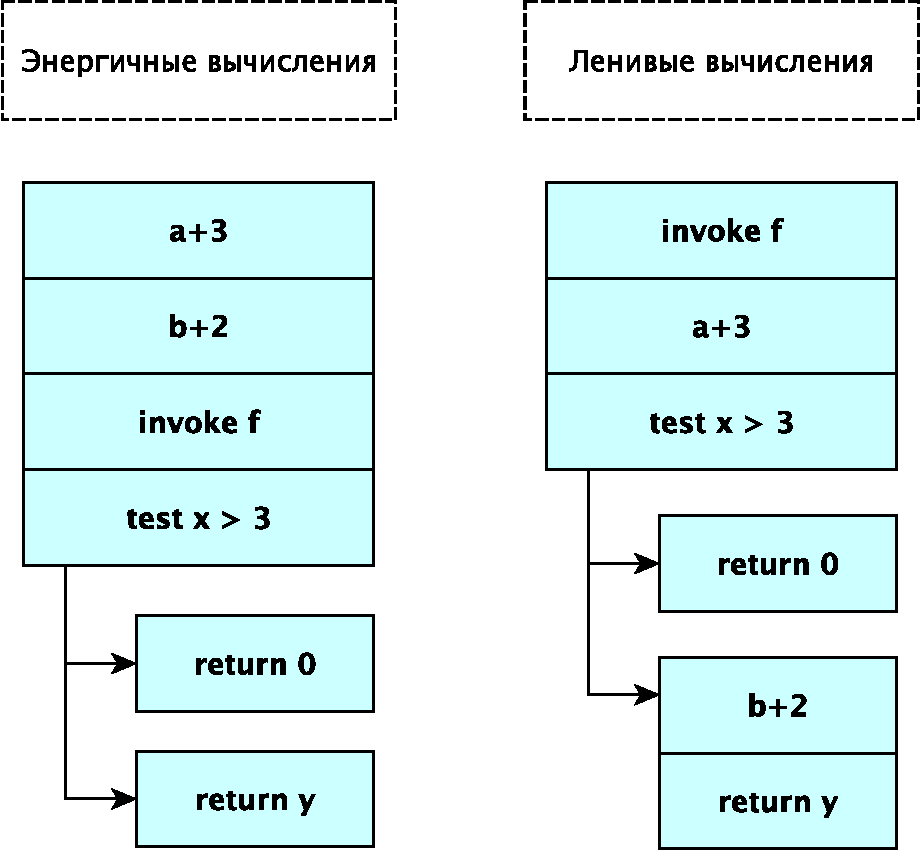
\includegraphics[width=0.6\textwidth]{illustrations/lazyorder-crop.pdf}
\caption{Ленивые и энергичные вычисления}
\label{fig:lazy_calc}
\end{figure}

Видно, что при ленивых вычислениях, реальное вычисление результата выражения откладывается насколько это возможно. Это создает свои проблемы: скажем передавать в функцию такое недосчитанное выражение гораздо сложнее, чем передать посчитанное заранее число. Поэтому ленивые вычисления в C++ встречаются только в двух контекстах:

\begin{enumerate}
\item В вычислениях с длинными логическими операциями: \lstinline!&&! и \lstinline!||!. Из-за ленивого порядка их применения, легальны выражения вида:
\begin{lstlisting}
if (p && p->next) { /* ... */ }
\end{lstlisting}
Если бы порядок вычисления был энергичным, то при нулевом указателе второе условие взорвалось.
\item В инстанцировании шаблонов
\end{enumerate}

Второй пункт создает столько неочевидных преимуществ, что дальше речь пойдёт в основном о нём.

\subsubsection{Инстанцирование шаблонов}\label{Templateinstancing}

Выше уже несколько раз было употреблено слово ``инстанцирование''. Интуитивно оно понятно, но оно имеет разный смысл для обычных классов (там инстанцирование класса это создание его объекта) и для шаблонов. Настало время дать этому слову более точное определение.

\textbf{Шаблонным инстанцированием} называется процесс порождения типов и функций из обобщённых шаблонных определений.

Инстанцирование может также включать в себя вывод типов для шаблонных параметров (type inference), изобретение типов обобщенных лямбда функций (type invention) и в конце всегда включает подстановку шаблонных параметров (type substitution).

В книгах по шаблонам, таких как \cite{vandervoord} традиционно много места отводится тому, что называется ``Separation model''\index{Separation model}. Это модель инстанцирования, когда код шаблона находится в одной единице трансляции, а инстанцирование происходит в другой. Начиная с C++11 экспорт шаблонов был запрещён, а Separation model объявлена устаревшей. Поэтому везде далее можно полагать, что код шаблона размещается и инстанцирование происходит в одной единице трансляции.

Ключевой точкой инстанцирования является подстановка типов. Именно корректная подстановка типов определяет в конечном итоге сигнатуру порожденной из шаблона функции.

Самое важное, что нужно знать про подстановку -- она по стандарту обязано работать лениво. Это означает, что проверены на корректность будут только те части шаблона, которые действительно были использованы в коде.

Пример вроде бы нарушает стандарт

\begin{lstlisting}
template <int N>
class Danger {
public:
  typedef char block[N]; 
};

template <typename T, int N>
class Tricky {
public:
  void test_lazyness() {
      Danger<N> no_boom_yet;
  }
};

int main(void)
{
  Tricky<int, -2> ok;
  return 0;
}
\end{lstlisting}

Несмотря на то, что инстанцирование определяет \lstinline!typedef! с некорректным параметром размера массива, это не является ошибкой, поскольку реально этот зависимый тип нигде не был использован. Ленивость вынуждает компилятор откладывать инстанцирование любой части шаблона так долго, как это возможно.

\subsubsection{Идиома SFINAE}\label{SFINAE}

\hfill\textit{I can accept failure, everyone fails at something.}

\hfill\textit{But I can't accept not trying.}{\vspace{0.5em}}

\hfill\textit{-- Michael Jordan}

Одной из важнейших идиом в правилах инстанцирования является SFINAE, что означает \textbf{substitution failure is not an error}. Она означает, что неудача при подстановке шаблонных параметров сама по себе не является ошибкой.

То, что я перевожу как ``неудача'' подстановки (substitution failure) это на самом деле термин, означающий скорее невозможность, то есть в слове failure нет оттенка недетерминированности, который, увы, есть в слове неудача. При чтении это надо понимать. 

Неудачную подстановку можно продемонстировать на примере уже полюбившейся всем функции максимума:

\begin{lstlisting}
template <typename T> inline const T
max (const T a, const T b)
{
  return (a > b) ? a : b;
}
\end{lstlisting}

Семантически здесь указано, что оба аргумента имеют одинаковый тип. Таким образом, подстановка, в которой для них будут выведены разные типы, будет неудачной.

\begin{lstlisting}
int g = max (1, 1.0);
\end{lstlisting}

Что произойдёт? Благодаря принципу SFINAE, наткнувшись на неудачную подстановку, компилятор не будет паниковать и выдавать сообщения об ошибках. Возможно где-то определён более подходящий шаблон, например:

\begin{lstlisting}
template <typename T, typename U> inline const T 
max (const T a, const U b) { ... }
\end{lstlisting}

и подстановка в него завершится успехом.

Если нет, то сообщение об ошибке будет выглядеть довольно очевидно:

\begin{verbatim}
error: no matching function for call to ‘max(int, double)’
note: candidate is:
note: template<class T> const T max(T, T)
note: template argument deduction/substitution failed:
note: deduced conflicting types for parameter 
     ‘T’ (‘int’ and ‘double’)
\end{verbatim}

Ещё один пример неудачной подстановки -- порождение кода, не соответствующего типу данных. Например ниже у выведенного типа \lstinline!int*! явно нет зависимого подтипа \lstinline!ElementT!.

\begin{lstlisting}
template<typename T>
typename T::ElementT at (T const& a, int i) {
  return a[i];
}

int
f (int *p) {
  int x = at(p, 7); /* boom! */
  return x;
}
\end{lstlisting}

Но само по себе это тоже не ошибка. С другой стороны, здесь конечно сложно предложить как следует переписать код, чтобы специализировать функцию для правильной подстановки. 

Очевидный вариант:

\begin{lstlisting}
template<typename T, typename U>
U at (T const& a, int i) {
  return a[i];
}
\end{lstlisting}

Не работает, потому что компилятору неоткуда вывести тип \lstinline!U!.

Более интересный вариант использует новый стандарт и не требует наличия зависимых типов:

\begin{lstlisting}
template<typename T>
auto at (T const& a, int i) -> decltype(a[i]) {
  return a[i];
}
\end{lstlisting}

Здесь подстановка пройдет удачно. Интересно, что стандарт не допускает перегрузку функции по возвращаемому значению, но допускает перегрузку шаблонной функции по возвращаемому значению \textbf{и типу}.

SFINAE является очень мощной техникой, позволяющей делать интересные вещи. Например определить на этапе компиляции имеет ли некий тип вложенный зависимый тип с определённым именем.

\lstinputlisting{cpp_code/p3s7.cpp}

Этот код выведет результат \lstinline!foo: 1, bar: 0!, верно определив наличие зависимого типа \lstinline!foo::foobar! в \lstinline!foo! и его отсутствие в \lstinline!bar!. Эта техника может казаться с первого взгляда не очевидной. Я рекомендую изучить идею, пока она не станет ясна: понимание SFINAE это ключ к пониманию всего метапрограммирования.

\subsubsection{Некоторые применения SFINAE}

Из всевозможных применений принципа SFINAE, два оказались исторически настолько важны, что были внесены в стандарт. Это \lstinline!static_assert! и \lstinline!enable_if! и о них следует поговорить подробнее.

В реалиях 98-го года \lstinline!static_assert! можно было бы реализовать следующим образом (идея Александреску):

\begin{lstlisting}
template <bool cond> struct static_assert;

template <> struct static_assert<true> {};
\end{lstlisting}

Эти две строчки поражают воображение своей элегантностью. К сожалению, static assertion failure в таком виде получается почти нечитаемой, поэтому жизнь вносит коррективы. В частности в C++11 используется функция двух аргументов: \lstinline!static_assert(cond, message)!. Поскольку такая проверка ничего не стоит на этапе выполнения, с ней нельзя перестараться:

\begin{lstlisting}
#include "mylib.h"
static_assert (MyLib::Version > 2, "Old Mylib");
static_assert (sizeof(int) == 4, "Incompatible environment");
// ..... etc
\end{lstlisting}

Если что-то можно проверить статически, лучше проверить это статически.

В тех же реалиях 98-го, \lstinline!enable_if! также записывается для работы через SFINAE:

\begin{lstlisting}
template<bool b, typename T = void>
struct enable_if {};

template <typename T>
struct enable_if<true, T> 
{
  typedef T type;
};
\end{lstlisting}

Тут очевидно, что в случае провала условия, в структуре не оказывается зависимого типа:

\begin{lstlisting}
template <typename T>
typename enable_if<sizeof(T) > 4, T>::type
foo (T x) 
{ 
// .....
}
\end{lstlisting}

Эта перегрузка \lstinline!foo! не сработает для неправильных типов.

В новом стандарте синтаксис \lstinline!enable_if! был сохранен. Это довольно мощная техника, но получающийся после её многократного применения код иногда оказывается куда менее читабельным, чем хотелось бы.

Фантастический пример использования \lstinline!enable_if! для создания условного \lstinline!explicit! был рассмотрен Стефаном Лававеем в его докладе на CppCon 2016.

\pagebreak
\subsection{Другие шаблонные параметры}

До сих пор рассматривались только параметризация шаблонов типами и немного -- целыми числами. Это не вполне исчерпывает возможности шаблонов. Они могут быть параметризованы указателями и даже другими шаблонами. Кроме того, можно увидеть, что по сути параметризация целыми, указателями, шаблонами -- это одна и та же параметризация. Ниже будут систематично рассмотрены все упомянутые случаи.

\subsubsection{Связь целых чисел и типов}\label{IntToype}

Следующая конструкция была предложена Александреску и использует возможность параметризации шаблона типом для создания в C++ перечислимых типов:

\begin{lstlisting}
template <int I>
struct Int2Type
{
  enum { value = I };
};
\end{lstlisting}

Обратите внимание, что \lstinline!Int2Type<0>!, \lstinline!Int2Type<1>!, \lstinline!Int2Type<2>! и так далее являются разными типами, при этом каждый содержит в себе информацию о своем порядковом номере. Идею можно расширить до почти полноценных нумералов:

\begin{lstlisting}
template <int I>
struct Int2Type
{
  enum { value = I };
  typedef int value_type;
  typedef Int2Type<I> type;
  typedef Int2Type<I+1> next;
  typedef Int2Type<I-1> previous;
};
\end{lstlisting}

Простой пример использования это сортировка массива:

\begin{lstlisting}
template <typename T, unsigned int N>
class Array 
{
private:
  enum AlgoType { NOOP, INSRT, QUICK };
  static const int algo = (N==0) ? NOOP : 
                          (N==1) ? NOOP :
                          (N<50) ? INSERTION_SORT : QUICK_SORT;
  void do_sort (Int2Type<INSRT>) { /* INSERTION_SORT */ }
  void do_sort (Int2Type<QUICK>) { /* QUICK_SORT */ }
public:
  /* ... all array-related stuff ... */
  void sort()
  {
    do_sort (Int2Type<algo>());
  }
};
\end{lstlisting}

Здесь пользователь вызывает только функцию \lstinline!sort!, которая, в зависимости от длины массива, сама решает какой алгоритм сортировки ей применить.

\subsubsection{Параметризация шаблонов указателями}\label{PointerTemplateArguments}

Понять каким образом происходит параметризация шаблонов указателями, поможет несколько синтетическая задача сопоставить каждой глобальной переменной в программе уникальное имя:

\begin{lstlisting}
template <int *foo>
class VariableNamer {
public:
  static const char *name;
};

int baz = 7;
int bar = 42;

template<>
const char * VariableNamer< &baz >::name = "baz";

template<>
const char * VariableNamer< &bar >::name = "bar";

template <int *foo> void
detect_global (void)
{
  printf ("called with: %s = %d\n", 
    VariableNamer<foo>::name, *foo);
}

int
main( int argc, char ** argv )
{
  baz = baz / 2;
  bar = bar + baz;
  detect_global <&bar> ();
  detect_global <&baz> ();
  return 0;
}
\end{lstlisting}

Шаблонный класс \lstinline!VariableNamer! здесь позволяет создать уникальный тип для каждой глобальной переменной и сохранить внутри присвоенное ей символьное имя. Пользующийся им шаблон \lstinline!detect_global! печатает имя переданной ему глобальной переменной и её значение.

В этом коде есть ряд недочетов, скажем его нельзя расширить для трэкинга локальных переменных, сложно обобщить на указатели на произвольный тип и так далее.

\textbf{Домашняя наработка:} подумайте как существенно улучшить \lstinline!VariableNamer!, не бойтесь при этом использовать препроцессор.

\subsubsection{Шаблонные шаблонные параметры\index{template template parameters}}\label{TemplateTemplateArguments}

Представьте, что вы используете CRTP для предоставления ``интерфейса'' к набору дочерних шаблонов, при этом как родитель, так и потомки параметризованы:

\begin{lstlisting}
template <typename derived, typename value> class interface {
    void do_something(value v) {
        static_cast<derived*>(this)->do_something(v);
    }
};

template <typename value> class derived : 
  public interface<derived<value>, value> {
    void do_something(VALUE v) { ... }
};

typedef interface<derived<int>, int> derived_t;
\end{lstlisting}

Строчка, определяющая \lstinline!derived_t! содержит неприятное дублирование типа  \lstinline!int!, который на самом деле один и тот же и для потомка и для предка. Мало того это даёт возможность ошибки при опечатке. Чтобы явно отобразить, что шаблон параметризуется зависимым параметризованным типом:

\begin{lstlisting}
template <template <typename> class derived, typename value> 
class interface {
    void do_something(value v) {
        static_cast<derived<value>*>(this)->do_something(v);
    }
};

template <typename value> class derived : 
  public interface<derived, value> {
    void do_something(value v) { ... }
};

typedef interface<derived, int> derived_t;
\end{lstlisting}

Обратите внимание на \lstinline!template <typename> class derived! -- именно такой синтаксис внутри списка аргументов показывает, что \lstinline!derived! это шаблонный тип, специфицированный неким зависимым. Александреску\cite{mcpp} использует шаблонные шаблонные параметры для реализации policy-классов

\begin{lstlisting}
template <template <typename> class CreationPolicy>
class WidgetManager : public CreationPolicy<Widget>
{
   ...
};
\end{lstlisting}

Считается, что \lstinline!WidgetManager! ``знает'' о том, что ему нужна \lstinline!CreationPolicy! именно для \lstinline!Widget!. При этом нужно понимать, что если шаблонный шаблонный класс параметризован более чем одним зависимым аргументом, это должно быть явно указано:

\begin{lstlisting}
template <template <typename, typename> class CreationPolicyEx>
class WidgetManager : 
  public CreationPolicyEx<Widget, WidgetPattern>
{
   ...
};
\end{lstlisting}

Разумеется, явно может быть указано сколько угодно зависимых типов.

Дополнительно можно рассмотреть трюк с прокси-данными, который позволяет динамически выбрать зависимый тип для вложенных в шаблон данных

\begin{lstlisting}
template<typename T, template<typename> class C>
struct A {
  typename C<T>::type data;  /* trick to use a proxy */
};
\end{lstlisting}

\subsubsection{CRTP с закрытой базой и ещё немного дружбы}\label{ClosedCRTP}

При использовании CRTP с закрытой базой (являющейся специализацией шаблонного шаблонного параметра), бывает полезно объявить закрытую базу другом, чтобы дать ей доступ к своей закрытой части.

Пусть по условию есть много конкретных транспортов, каждый из которых содержит метод с известным именем и сигнатурой:

\begin{lstlisting}
template<typename Service>
class tcp {
public:
    void send(....) {

    }
};
\end{lstlisting}

\begin{lstlisting}
template<typename Service>
class udp {
public:
    void send(....) {

    }
};
\end{lstlisting}

Тогда сервис, предназначенный для параметризации конкретным транспортом, но при этом сам транспортом не являющийся, может с одной стороны наследовать транспорту закрыто (отношение part-of) а с другой стороны объявлять его другом.

\begin{lstlisting}
/* Transport<service> is implementation detail */
template<template<typename> class Transport>
class service : private Transport<service> {
    /* since we derive privately, make the transport layer a 
       friend, so that it can cast its this pointer down */
    friend class Transport<service>;
public:
    typedef Transport<service> transport_type;
    /* common code */
    void do_something(....) { 
        send(....);
    }
};
\end{lstlisting}

И именно это даёт ему возможность вызывать его методы как родные, одновременно пряча их от вызова извне.

Типичное применение:

\begin{lstlisting}
typedef service<tcp> service_tcp;
typedef service<udp> service_udp;
\end{lstlisting}

\textbf{Вопрос к студентам:} как переписать \lstinline!do_something! если закрытая база не сделана другом?

\ifanswers
Как вариант: \lstinline!transport_type::send(....);!
\fi

\pagebreak
\subsection{Метапрограммы\index{Metaprogramming}}

Шаблонное метапрограммирование было открыто в 1994-м году. Эрвин Анрух (Erwin Unruh) на заседании комитета по стандартизации сделал доклад, из которого следовало, что шаблоны могут быть использованы для вычисления на этапе компиляции и продемонстрировал генератор простых чисел, который на этапе компиляции выводил в виде сообщений об ошибках простые числа от 2 до заранее заданного настраиваемого предела. Но этот генератор довольно сложен. Кроме того, метапрограммирование использует несколько иной подход к вычислениям, с которого и следует начать.

\subsubsection{Две модели вычислений}\label{ComputationModels}

Представьте простую функцию, вычисляющую факториал числа. Человек с опытом на C написал бы её в итеративном стиле:

\begin{lstlisting}
int
fact_0 (int x)
{
  int i, res = 1;
  for (i = 2; i <= x; ++i)
    res *= i;

  return res;
}
\end{lstlisting}

Здесь для того, чтобы вычислить факториал понадобились две ячейки памяти -- изменяемые переменные \lstinline!i! и \lstinline!res!. Математик Алан Тьюринг в 1936-м году опубликовал статью из которой следовало, что очень сложные вычислительные процессы можно произвести, имея в своем распоряжении:

\begin{itemize}
\item ветвления (скажем оператор \lstinline!if! или тернарный оператор)
\item переходы (хороший пример -- любой цикл или простое \lstinline!goto!)
\item последовательное линейное исполнение инструкций
\item достаточное количество изменяемой памяти
\end{itemize}

Факториал переписанный в более Тьюринг-стиле, но все ещё на C показывает некий минимализм выразительных средств:

\begin{lstlisting}
int memory[3];

/* memory[0] is input and result */
fact_0:
  memory[1] = 1;
  memory[2] = 1;
  label t, fin;
t:
  memory[1] += 1;
  memory[2] *= memory[1];
  if (memory[1] > memory[0]) 
    goto fin;
  goto t;
fin:
  memory[0] = memory[2];
\end{lstlisting}

Некоторое время спустя, Стивен Клини обнаружил, что очень сложные вычислительные процессы можно произвести, имея в своем распоряжении:

\begin{itemize}
\item ветвления (скажем оператор \lstinline!if! или тернарный оператор)
\item вызовы функций с передачей аргументов
\end{itemize}

В этом случае вообще не требуется изменяемых переменных.

И правда, факториал можно записать иначе:

\begin{lstlisting}
int
fact_1 (int x)
{
  if (x < 2)
    return x;
  else
    return x * fact_1 (x - 1);
}
\end{lstlisting}

Такие функции были им названы \textbf{частично-рекурсивными} функциями и было доказано, что аппарат частично-рекурсивных функций эквивалентен по вычислительной мощности машинам Тьюринга и лямбда-выражениям

Порождаемый таким образом рекурсивный процесс вычислительно не слишком эффективен, поскольку выражение \lstinline!x * fact_1 (x - 1)! не может быть вычислено до полного вычисления всех рекурсивных вызовов. Таким образом нет аккумулятора (вернее он неявно размазан по рекурсивной цепочке). Аккумулятор тоже можно сымитировать, изменив факториал:

\begin{lstlisting}
int
fact_2_1 (int x, int idx, int product)
{
  if (idx > x)
    return product;
  else
    return fact_2_1 (x, idx + 1, product * idx);
}

int
fact_2 (int x)
{
  return fact_2_1 (x, 1, 1);
}

\end{lstlisting}

Интересно, что обычные программы на C++ больше похожи на подсахаренные машины Тьюринга (с поправкой на структурное программирование, взрослые циклы и вызовы функций). А вот метапрограммирование больше напоминает подход Клини.

\subsubsection{Простая рекурсия и арифметика}\label{SimpleRecursion}

\hfill\textit{To iterate is human, to recurse divine}{\vspace{0.5em}}

\hfill\textit{-- L. Peter Deutsch}

Начать рассмотрения метапрограммирования следует с простой рекурсии и арифметики. 

\textbf{Задача:} вычислить N-ю степень числа 3

Пока что ведь неочевидно, что на шаблонах во время компиляции можно даже это. Всегда первый шаг: переписать в функциональном стиле

\begin{lstlisting}
int
three_to_n (int n)
{
  if (n == 0)
    return 1;
  else
    return 3 * three_to_n (n - 1);
}
\end{lstlisting}

Теперь вычислить N-ю степень числа 3 на этапе компиляции довольно просто:

\begin{lstlisting}
/* primary template to compute 3 to the Nth */
template<int N> 
struct Pow3 { 
  enum { result=3*Pow3<N-1>::result }; 
}; 

/* full specialization to end the recursion */
template<> 
struct Pow3<0> { 
  enum { result = 1 }; 
}; 

int main() 
{ 
    std::cout << "Pow3<7>::result = " << Pow3<7>::result 
              << '\n'; 
} 
\end{lstlisting}

Здесь значение \lstinline!Pow3<7>::result! будет вычислено до выполнения программы на этапе компиляции и впечатано в генерированный ассемблер как число. Давайте посмотрим по пунктам как это работает.

\begin{enumerate}
\item
\lstinline!Pow3<7>::result! раскрывается как \lstinline!3*Pow3<6>::result! и так далее до \lstinline!3*3*3*3*3*3*3*Pow3<0>::result!
\item
Для \lstinline!Pow3<0>::result! срабатывает частичная специализация и он превращается в \lstinline!1!
\item
Итого, в код будет после раскрытия шаблонов записано:
\begin{lstlisting}
int main() 
{ 
    std::cout << "Pow3<7>::result = " << 3*3*3*3*3*3*3*1                                         
              << '\n'; 
} 
\end{lstlisting}
\end{enumerate}

Это и выведет тривиально правильный результат. Пример специально подобран так, что написать в коде \lstinline!Pow3<7>::result! занимает столько же символов, сколько итоговая строчка. Выгода здесь в читабельности кода (общий смех). 

\textbf{Вопрос к студентам:} теперь кто напишет факториал?

\ifanswers
Ответ: скорее всего будет по аналогии со степенью, хотя могут быть взбрыки у неглупых групп.
\fi

Возможно ответ был такой:

\begin{lstlisting}
template <int n>
struct factorial 
{
  enum { value = n * factorial<n - 1>::value };
};
 
template <>
struct factorial<0> {
  enum { value = 1 };
};
\end{lstlisting}

Можно посмотреть эту метапрограмму в специальной утилите metashell:

\begin{verbatim}
$ metashell
> #include <metashell/scalar.hpp>
> #include "meta-fact.hpp"
> #msh mdb factorial<6>::value
Metaprogram started
(mdb) ft
factorial<6>::value
+ factorial<6> 
| + factorial<5> 
| | + factorial<4> 
| | | + factorial<3> 
| | | | + factorial<2> 
| | | | | + factorial<1> 
| | | | | | + factorial<0> 
| | | | | | ` factorial<0>::(anonymous) 
| | | | | ` factorial<1>::(anonymous) 
| | | | ` factorial<2>::(anonymous) 
| | | ` factorial<3>::(anonymous) 
| | ` factorial<4>::(anonymous) 
| ` factorial<5>::(anonymous) 
` factorial<6> 
(mdb) quit
> #msh quit
\end{verbatim}

Видно, что это так себе факториал. Гораздо более интересный итеративный процесс получается из следующего подхода:

\begin{lstlisting}
template <int n, int idx, int product>
struct fact_rec
{
  enum { 
    value = fact_rec <n, idx + 1, product * idx>::value
  };
};

template <int n, int product>
struct fact_rec <n, n, product>
{
  enum { value = product * n };
};

template <int n>
struct factorial2
{
  enum { value = fact_rec <n, 1, 1> :: value };
};
\end{lstlisting}

Тот же metashell выдает куда более приглядную картинку.

\begin{verbatim}
Metaprogram started
(mdb) ft
factorial2<6>::value
+ factorial2<6> 
| ` fact_rec<6, 2, 1> 
|   ` fact_rec<6, 3, 2> 
|     ` fact_rec<6, 4, 6> 
|       ` fact_rec<6, 5, 24> 
|         ` fact_rec<6, 6, 120> 
` factorial2<6> 
\end{verbatim}

На самом деле, количество инстанцирований не уменьшилось, но работа компилятору сильно упростилась. Кроме того, можно обратить внимание, что попутно были вычислены все факториалы и их список 1, 2, 6, 24, 120 находится в явном виде перед глазами.

\textbf{Домашння наработка:} сделать числа Фибоначчи на шаблонах: с тупой древовидной рекурсией и более умные. Посмотреть разницу во времени компиляции.

\subsubsection{Ветвления и пример квадратного корня}\label{TemplateIfElse}

Обычная шаблонная специализация позволяет проверять только равенство. В метапрограммах можно делать также ветвления if-then-else\index{if-then-else template} с любыми, сколь угодно сложными условиями. Напишем простой шаблон:

\begin{lstlisting}
/* primary template: yield second or third argument, 
   depending on first argument */
template<bool C, typename Ta, typename Tb> 
struct IfThenElse; 

/* partial specialization: true yields second argument */
template<typename Ta, typename Tb> 
struct IfThenElse<true, Ta, Tb> 
{ 
  typedef Ta ResultT; 
}; 

/* partial specialization: false yields third argument */
template<typename Ta, typename Tb> 
struct IfThenElse<false, Ta, Tb> 
{ 
  typedef Tb ResultT; 
}; 
\end{lstlisting}

С помощью этого шаблона теперь можно легко написать, например, вычисление целочисленного квадратного корня во время компиляции.
И опять первый шаг: прикинуть код на C++ в функциональном стиле:

\begin{lstlisting}
int
isqrt (int N, int lo = 1, int hi = N)
{
  int mid = (lo + hi + 1) / 2;

  if (lo == hi)
    return lo;
  else
    {
      if (N < mid * mid)
        return isqrt (N, lo, mid - 1);
      else
        return isqrt (N, mid, hi);
    }
}
\end{lstlisting}

Теперь его можно перевести на шаблоны

\begin{lstlisting}
/* primary template for main recursive step */
template <int N, int LO = 1, int HI = N> 
struct Sqrt 
{ 
  /* compute the midpoint, rounded up */
  enum { mid = (LO+HI+1)/2 }; 

  /* search a not too large value in a halved interval */
  typedef typename IfThenElse<(N<mid*mid), 
                               Sqrt<N,LO,mid-1>, 
                               Sqrt<N,mid,HI> >::ResultT 
          SubT; 
  enum { result = SubT::result }; 
}; 

/* partial specialization for end of recursion criterion */
template <int N, int S> 
struct Sqrt <N, S, S> 
{ 
  enum { result = S }; 
}; 
\end{lstlisting}

Рассмотренные примеры показывают, что в метапрограммах можно делать ветвления и циклы (через рекурсию), хранить промежуточные данные и выполнять над ними основные арифметические операции. Всего этого достаточно для того, чтобы доказать Тьюринг-полноту шаблонов C++\index{Turing completeness of templates}.

\subsubsection{Простые числа}\label{TemplatePrimes}

Благодаря вложенным классам, можно устраивать некую модульность в вычислениях и даже писать нечто, похожее на ``метаподпрограммы''. Большой пример с простыми числами сильно отличается от базового кода Анруха (его всегда можно найти в интернетах), но он несколько полезней, так как результаты печатаются не в виде ошибок, а доступны для использования.

\begin{lstlisting}
template <int i>
struct NthPrime
{
  template <int p>
  struct is_prime
  {
    template <int n>
    struct n_divisors
    {
      template <int N, int M>
      struct is_divisor
      {
        enum { val = is_divisor <N, M - 1>::val + ((N % M) == 0) };
      };

      template <int N>
      struct is_divisor <N, 1>
      {
        enum { val = 0 };
      };

      enum { val = is_divisor <n, n - 1>::val };
    };
    enum { val = (n_divisors <p>::val == 0) };
  };

  template <int n, int m>
  struct search_step
  {
    enum { val = search_step <n - (is_prime <m>::val), m + 1>::val };
  };

  template <int m>
  struct search_step <1, m>
  {
    enum { val = m - 1 };
  };

  enum { val = search_step <i, 3>::val };
};
\end{lstlisting}

Использование очевидно:

\begin{lstlisting}
int main(int argc, char* argv[])
{
  printf("Prime 6: %i\n", NthPrime<6>::val);
  return 0;
}
\end{lstlisting}

\textbf{Домашняя наработка:} коды Грея на шаблонах

\pagebreak
\subsection{Определители и модификаторы типов}

Метапрограммы, работающие над целыми числами, являются хорошей наработкой техники, но в реальности мало распространены. Никто не будет в разы замедлять компиляцию ради списка кодов Грея -- их сгенерят скриптом и подключат отдельным заголовочником, если уж очень надо. Настоящее применение метапрограмм -- работа над типами.

\subsubsection{Стой, кто идёт?\index{Type traits}}\label{TypeTraits}

Новый стандарт предлагает большое количество удобных стандартных шаблонов для получения более детальной информации о типах на этапе компиляции. 

Большинство из них должны как-то сообщать ответы ``да'' и ``нет'' на вопросы ``является ли это тем-то и тем-то?'', скажем: ``является ли тип аргумента указателем на функцию-член класса X с такой-то сигнатурой?''. Чтобы закодировать ответы, используется обертка над интегральными константами времени компиляции:

\begin{lstlisting}
template <typename T, T v>
struct integral_constant;
\end{lstlisting}

Теперь можно определить \lstinline!true_type! как \lstinline!integral_constant<bool, true>! и \lstinline!false_type! как \lstinline!integral_constant<bool, false>!.

Можно продемонстрировать создание пользовательских констант:

\begin{lstlisting}
typedef integral_constant<int, 2> two_t;
typedef integral_constant<int, 4> four_t;
static_assert (two_t::value * two_t::value == four_t::value, 
               "2*2 != 4");
\end{lstlisting}

Метапрограммирование на интегральных константах выглядит небезынтересно:

\begin{lstlisting}
template<size_t N>
struct fibonacci : 
    integral_constant< size_t, 
                       fibonacci<N-1>{} + 
                       fibonacci<N-2>{}> {};

template<> struct fibonacci<1> : 
    integral_constant<size_t,1> {};

template<> struct fibonacci<0> : 
    integral_constant<size_t,0> {};
\end{lstlisting}

Используя закодированные интегральными константами истину и ложь, можно сварганить простейший из определителей типов: является ли анализируемый тип интегральным (это такие типы как \lstinline!bool!, \lstinline!char!, \lstinline!short!, \lstinline!int!, \lstinline!long!, \lstinline!long long! и все их cv-квалификации). Как пример использования: можно потребовать интегрального \lstinline!T! в шаблонной функции (пока нет концептов, вполне себе концепт для бедных).

\begin{lstlisting}
template <typename T>
T f(T i)
{
    static_assert(std::is_integral<T>::value, 
                  "Integer required");
    return i;
}
\end{lstlisting}

\textbf{Домашняя наработка:} как могла бы выглядеть реализация \lstinline!is_integral! и \lstinline!is_floating_point!?

Имея два определителя, можно скомбинировать из них производные, скажем:

\begin{lstlisting}
template <typename T>
struct is_arithmetic : std::integral_constant<bool,
  std::is_integral<T>::value ||
  std::is_floating_point<T>::value> {};
\end{lstlisting}

Можно потренироваться и определить является ли нечто указателем:

\begin{lstlisting}
template <typename T> 
struct is_pointer_helper : std::false_type {};

template <typename T> 
struct is_pointer_helper<T*> : std::true_type {};

template <typename T> struct is_pointer : 
    is_pointer_helper <typename std::remove_cv<T>::type> {};
\end{lstlisting}

Обратите внимание на использование \lstinline!remove_cv!, который сам является композитным хелпером из \lstinline!remove_const! и \lstinline!remove_volatile! которые по отдельности тоже не составляют проблем.

\textbf{Вопрос к студентам:} как бы вы реализовали \lstinline!remove_const!? 

\ifanswers
Правильный ответ:

\begin{lstlisting}
template <typename T> 
struct remove_const { typedef T type; };
template <typename T> 
struct remove_const<const T> { typedef T type; };
\end{lstlisting}
\fi

Полное рассмотрение всех возможных traits не нужно -- они перечислены в стандарте и их несложно конструировать по мере необходимости. Можно запомнить (это примерно столь же полезная для запоминания информация как первый 21 знак числа пи), что все что угодно, что встречается в корректной программе на C++14 может быть отнесено к одному из 14 базовых классов traits и только к нему одному. И кстати 14 это первые две цифры номера стандарта. Совпадение? Не думаю.

\subsubsection{Ваш третий лучший друг}\label{FriendUsing}

До сих пор двумя лучшими (воображаемыми) друзьями программиста были \lstinline!typedef! (\ref{FriendTypedef}) и \lstinline!typename! (\ref{FriendTypename}). Но теперь оказывается, что в новом стандарте у \lstinline!typedef! есть младший братик \lstinline!using!

\begin{lstlisting}
typedef int MyInt;
using MyInt = int;
\end{lstlisting}

Эти две строчки совершенно эквивалентны. Зачем же нужно было вводить новое ключевое слово? Потому что \lstinline!using! умеет больше:

\begin{lstlisting}
template <typename T> 
using MyType = AnotherType< T, MyAllocatorType >; 

template <typename T> 
using ptr = T*;
...
MyType<int> a;
ptr<int> x;
\end{lstlisting}

Очень удобно совмещать новый \lstinline!using! с определителями типов. Например такое переопределение, как приведенное ниже:

\begin{lstlisting}
template <typename T> using decay_t = typename decay<T>::type;
\end{lstlisting}

Позволяет сделать in-place сгнивалку для типов. Синонимы для всех распространенных определителей уже включены в стандарт.

В вашей стандартной библиотеке даже базовые типы могут быть определены исходя из реалий архитектуры:

\begin{lstlisting}
using size_t = decltype(sizeof(0));
using ptrdiff_t = decltype((int*)0 - (int*)0);
using nullptr_t = decltype(nullptr);
\end{lstlisting}

Кстати, это даёт замечательный пример совмещения \lstinline!using! и \lstinline!decltype!

\textbf{Обсуждение в аудитории:} почему не был расширен синтаксис уже имевшегося \lstinline!typedef!, а было перегружено ключевое слово \lstinline!using! которое вообще-то совсем о другом?

Тема и впрямь дискуссионная. Имеется частное мнение Саттера, что ``there is no type to define'' и \lstinline!typedef! показался комитету семантически непригодным для выражения идеи семейства типов. Ну ок.

\subsubsection{Вариабельные шаблоны для списков типов}

Выше (\ref{TypeTraits}) были упомянуты определители типов из стандартной библиотеки. Довольно легко определить (и не надо определять, так как он есть в стандарте) простой шаблон \lstinline!is_same! определяющий одинаковые ли типы переданы ему на вход:

\begin{lstlisting}
template<typename T, typename U>
struct is_same : std::false_type {};
 
template<typename T>
struct is_same<T, T> : std::true_type {};
\end{lstlisting}

Но вариабельные шаблоны предлагают намного большие возможности. Например с их помощью можно сделать определитель \lstinline!is_one_of! определяющий равенство данного типа одному из типов данного списка. Идея проста как правда:

\begin{lstlisting}
template<typename T, typename... List>
struct is_one_of;

template<typename T>
struct is_one_of<T> : false_type {};

template<typename T, typename... Tail>
struct is_one_of<T, T, Tail...> : true_type {};
\end{lstlisting}

Самое сложное и изящное это рекурсивный вызов:

\begin{lstlisting}
template<typename T, typename Head, typename... Tail>
struct is_one_of<T, Head, Tail...> : 
       is_one_of<Head, Tail...> {};
\end{lstlisting}

Таким образом вариабельные шаблоны позволяют рекурсию по списку типов гораздо естественней, чем это позволяли делать обычные шаблоны. Большое количество кода в известной книге \cite{mcpp} теперь может быть переписано гораздо проще.

\textbf{Вопрос к студентам:} Дан template parameter pack \lstinline!...Ts!, где каждый тип может быть либо \lstinline!true_type! или \lstinline!false_type!. Как узнать, являются ли они все \lstinline!true_type!?

Очевиден простой рекурсивный ответ:

\begin{lstlisting}
template <typename ...Ts>
struct all_true;

template <typename H, typename ...Ts>
struct all_true<H, Ts...> : 
       and_<is_same<true_type, H>, 
       all_true<Ts...>> {};

template <>
struct all_true<> : true_type {};
\end{lstlisting}

Можно ли сделать изящней, не инстанцируя $O(N)$ типов?

\ifanswers
Более просветляющий ответ использует кортежи:

\begin{lstlisting}
template <typename H, typename ...Ts>
struct all_true<H, Ts...> : 
       and_<is_same<true_type, H>, 
       is_same<tuple<H,Ts...>,
               tuple<Ts...,H>>> {};
\end{lstlisting}
\fi

TODO: вставить больше улучшенного метапрограммирования с учётом нового стандарта:
\url{http://www.pdimov.com/cpp2/simple_cxx11_metaprogramming.html}

Для комбинирования traits, в C++17 собираются ввести магические классы \lstinline!conjunction! и \lstinline!disjunction!, являющиеся вариабельными шаблонами и работающие как длинные логические операции -- то есть с сокращенным путём исполнения.

\pagebreak
\subsection{Вычисления времени компиляции}

\hfill\textit{Once you're const, you are ensconced}{\vspace{0.5em}}

\hfill\textit{-- Susan Powell}

Вычисления времени компиляции до выхода стандарта C++11 велись исключительно с помощью особой шаблонной магии, рассмотренной выше. В новом стандарте появился способ сделать это по человечески. Новое ключевое слово constexpr контролирует время выполнения выражения. Это позволяет создавать настоящие константы и константные выражения, заниматься метапрограммированием и многое другое. Здесь будут систематично рассмотрены все перечисленные возможности.

\subsubsection{Ещё раз о константности}\label{Constexpr}

Уже рассматривавшийся выше модификатор const служит для того, чтобы объявить некие данные неизменяемыми. Но когда этим не изменяемым данным будет в первый раз присвоено их (в дальнейшем окончательное) значение? It depends.

\begin{lstlisting}
const int MAXSIZE = numeric_limits<int>::max();
int arr[MAXSIZE]; /* not legal in C++ */
\end{lstlisting}

В этом примере значение максимального возможного целого будет присвоено MAXSIZE только в динамике. В результате на этапе компиляции, размер arr всё ещё неизвестен и строго соответсвующие стандарту C++ компиляторы могут выразить этим свое неудовольствие (такие массивы возможны в C и часто для C++ это включают как расширение).

Те же проблемы испытывают статические данные в классах и структурах:

\begin{lstlisting}
struct S 
{
  static const int sz;
};

const int page_sz = 4 * S::sz; /* dynamic init */

const int S::sz = 256; /* too late */
\end{lstlisting}

Это законная запись. Инициализатор статической константы, как и было рассмотрено ранее, должен появиться вне класса. Далее \lstinline!page_sz! будет инициализирвоана верным значением, но потребует инициализации времени выполнения. Как ни странно, но совсем немного отличающийся код уже пройдет инициадизацию на этапе компиляции:

\begin{lstlisting}
struct S 
{
  static const int sz = 256;
};

const int page_sz = 4 * S::sz; /* static init */

const int S::sz; /* ok */
\end{lstlisting}

Это довольно грустно и требует от программиста помнить все тонкие правила константности, что, конечно, нереально. Именно этим и было мотивировано введение в стандарт ключевого слова, делающего известность на этапе компиляции явной.

\subsubsection{Константно-выраженные функции}\label{Constexpr:functions}

Как вообще могла бы быть объявлена функция \lstinline!numeric_limits<int>::max()!? Например так:

\begin{lstlisting}
#define INT_MAX (2147483647)

template <>
struct numeric_limits<int> {
  static inline int max () { return INT_MAX; }
};
\end{lstlisting}

Эта функция -- прекрасный кандидат на формирование константного выражения. Она:
\begin{itemize}
\item не \lstinline!void!, то есть возвращает какое-то значение
\item состоит из одного \lstinline!return! -- то есть не заводит локальных переменных и не использует стек
\end{itemize}

Именно в таких двух условиях, функция в C++11 может быть сделана \textbf{константно-выраженной} для чего используется ключевое слово \lstinline!constexpr!.

\begin{lstlisting}
template <>
struct numeric_limits<int> {
  static constexpr int max () { return INT_MAX; }
};
\end{lstlisting}

Более интересный пример: что если сделать константно-выраженной обычную арифметичесмкую функцию?

\begin{lstlisting}
constexpr int square(int x) { return x * x; }
/* ... */
constexpr int res = square(5);
\end{lstlisting}

Здесь \lstinline!res! будет известен на этапе компиляции. Но при этом в таком виде:

\begin{lstlisting}
// foo's argument unknown at compile time
int foo (int y) { return square(y); }
\end{lstlisting}

Функция square (даже объявленная \lstinline!constexpr!) ведёт себя как самая обычная функция. Это позволяет иметь её одну, не заводя зоопарк \lstinline!constexpr! и не-\lstinline!constexpr! зверюшек.

В стандарте C++14 ослаблены ограничения на константно-выраженные функции. Начиная с этого стандарта, в такой функции могут содержаться:

\begin{itemize}
\item Все объявления, кроме \lstinline!static! и \lstinline!thread_local! переменных, а также неинициализированных переменных
\item Условные операции \lstinline!if! и \lstinline!switch!
\end{itemize}

Это делает написание таких функций гораздо более удобным. Например легальной становится следующая конструкция:

\begin{lstlisting}
constexpr int 
ipow (int x, int n) 
{ 
  int r = x;
  while (--n > 0) r *= x;
  return r;
}
\end{lstlisting}

Конечно это увеличивает работу для компилятора.

\subsubsection{Аннотация данных}\label{Constexpr:data}

Чтобы отличать обычные данные от известных на этапе компиляции, данные и даже члены классов тоже можно аннотировать \lstinline!constexpr!

\begin{lstlisting}
struct S
{
private:
  static constexpr int sz; // constexpr variable
public:
  constexpr int two(); //constexpr function
};

constexpr int S::sz = 256;
enum DataPacket
{
  Small=S::two(), // error (call before def)  
  Big=1024
};

constexpr int S::two() { return sz*2; }
constexptr S s;

int arr[s.two()]; // ok (call after def)
\end{lstlisting}

Видно, что по существу они мало чем отличаются от обычных данных. Но компилятор имеет насчёт них точную гарантию что их значения при компиляции уже известны.

\subsubsection{Темные чудеса шаблонных переменных}\label{Constexpr:templatevars}

В отличии от C++11, в C++14 разрешено делать шаблонными не только классы и функции, но и переменные:

\begin{lstlisting}
template <typename T> T n = T(5);

int 
main()
{
    n<int> = 10;
    std::cout << n<int> << " ";    // 10
    std::cout << n<double> << " "; // 5
}
\end{lstlisting}

Вместе с \lstinline!constexpr! аннотацией переменных, это позволяет вводить гораздо более симпатичные определители типов, рассмотренные в (\ref{TypeTraits}).

\begin{lstlisting}
template <typename T> 
constexpr bool is_void_v = is_void<T>::value;
\end{lstlisting}

Записывать \lstinline!is_void_v<T>! конечно гораздо проще и приятней, чем \lstinline!is_void<T>::value! (общий смех).

Но тогда возникает вопрос. Неужели у нас могут быть \lstinline!constexpr! данные типов \lstinline!int! или \lstinline!float!, но не может быть \lstinline!constexpr! данных пользовательских типов? Конечно могут.

\subsubsection{Аннотация конструкторов}\label{Constexpr:ctors}

Если у вас есть необходимость, чтобы ваш тип мог вести себя как compile-time константа, для него можно написать \lstinline!constexpr!-конструктор:

\begin{lstlisting}
struct Complex
{
  constexpr Complex(double r, double i) : 
    re(r), im(i) { }

  constexpr double real() const { return re;}
  constexpr double imag() const { return im;}
private:
 double re;
 double im;
};

constexpr complex c(0.0, 1.0);
\end{lstlisting}

Тело такого конструктора в C++11 обязано быть пустым, вся инициализация производится в списке инициализации. В C++14 это правило несколько ослаблено.

Для такого пользовательского класса можно ввести даже арифметику:

\begin{lstlisting}
struct Complex
{
  constexpr Complex(double r = 0.0, double i = 0.0) : 
    re(r), im(i) { }

  constexpr double real() const { return re;}
  constexpr double imag() const { return im;}

  constexpr Complex& operator+= (const Complex &rhs)
  {
    re += rhs.re;
    im += rhs.im;
    return *this;
  }

private:
  double re;
  double im;
};

constexpr Complex operator+ (const Complex &lhs, 
                             const Complex &rhs)
{
  Complex tmp = lhs;
  tmp += rhs;
  return tmp;
}
\end{lstlisting}

Но, конечно, всё это ООП времени компиляции является скорее изыском. Обычно такие абстракции в \lstinline!constexpr! не нужны и гораздо большее применение имеют пользовательские литералы.

\subsubsection{Пользовательские литералы}\label{Constexpr:userliterals}

Для определения пользовательского литерала, следует переопределить оператор кавычки.

\begin{lstlisting}
constexpr Complex operator "" _i( long double i )
{
  return Complex (0.0, i);
}
\end{lstlisting}

Теперь будет работать следующий код:

\begin{lstlisting}
  constexpr Complex c = 0.0 + 1.0_i;
\end{lstlisting}

Таким образом будет (на этапе компиляции!) создана константа пользовательского типа.

Строструп приводит даже более впечатляющий пример ( \url{http://www.stroustrup.com/Software-for-infrastructure.pdf} TODO: добавить в список литературы? ):

\begin{lstlisting}
template<int M, int K, int S> struct Unit {
       enum { m=M, kg=K, s=S };
};

template<typename Unit> 
struct Value {
  double val; 
  explicit Value(double d) : val(d) {}
};
\end{lstlisting}

Далее ряд синонимов для тензорных индексов размерности:

\begin{lstlisting}
using Meter = Unit<1,0,0>;
using Second = Unit<0,0,1>;
using Second2 = Unit<0,0,2>; 
using Speed = Value<Unit<1,0,-1>>; 
using Acceleration = Value<Unit<1,0,-2>>;
\end{lstlisting}

И пользовательские литералы для удобного обозначения констант.

\begin{lstlisting}
constexpr Value<Meter> operator"" m(long double d)
{
  return Value<Meter> (d);
}   

constexpr Value<Second> operator"" s(long double d)
{
  return Value<Second> (d);  
}   

constexpr Value<Second2> operator"" s2(long double d)
{
  return Value<Second2> (d); 
}
\end{lstlisting}

Написав соответствующие перегрузки операторов деления, далее можно добиться статической проверки типов в удобной форме:

\begin{lstlisting}
Speed sp1 = 100_m/9.8_s;  // ok
Speed sp2 = 100_m/9.8_s2; // error (m/s2 is acceleration)
Speed sp3 = 100/9.8_s;    // error (100 has no unit)
Acceleration acc = sp1/0.5_s; // ok again
\end{lstlisting}

\textbf{Домашняя наработка:} добейтесь работы строчки \lstinline!constexpr Kilogramm mass = 5_kg + 3_lb!, где lb это фунты, на этапе компиляции строящей преобразование фунтов в килограммы.

\pagebreak
\subsection{Домашняя наработка по шаблонам}

\textbf{Контрольные вопросы}

\begin{enumerate}
\item Чем отличается вывод типов шаблонами от вывода типов через auto/decltype?
\item Какие сложности вносит в разрешение перегрузки тот факт, что функция может быть шаблонной?
\item Как заставить компилятор инстанцировать шаблон функции для конкретного типа только один раз на все единицы трансляции?
\item Не нарушит ли шаблон функции в заголовочном файле ODR при инстанцировании везде куда включен заголовочник?
\item Чем отличается статический полиморфизм от динамического полиморфизма?
\item Может ли программа на C++ быть быстрее, чем такая же программа на C, реализующая тот же алгоритм?
\item Может ли шаблонный класс иметь несколько перегруженных конструкторов копирования?
\item Чем отличается полная специализация от частичной?
\item Как вы будете выбирать между специализацией и перегрузкой шаблонных функций?
\item Может ли быть полностью специализирован метод внутри определения частично специализированного класса?
\item В C++ нет частичной специализации функций. Можно ли сымитировать её средствами языка?
\item Возможен ли вывод типа при конструировании экземпляра шаблонного класса?
\item На каком этапе разрешаются зависимые имена в шаблонах классов?
\item Как внутри шаблонного класса сделать имя метода, не зависящего от шаблонных параметров, зависимым? Зачем это может быть нужно?
\item Можно ли сконструировать объект шаблонного типа при наличии конкурирующей специализации этого типа?
\item Можно ли в зависимости от шаблонного параметра изменить тип единственного поля в классе без частичной специализации этого класса?
\item Может ли шаблонная функция быть виртуальной?
\item Как расшифровывается CRTP, зачем нужна эта идиома?
\item Как в C++ происходит разрешение грамматической неоднозначности при использовании шаблонов?
\item Может ли вариабельный шаблон быть частично специализирован по части пачки параметров?
\item Перечислите все значения троеточия (ellipsis) в грамматике языка.
\item Можно ли раскрытием пачки параметров сформировать поля в классе?
\item В каких случаях пустая пачка параметров делает шаблонный класс не шаблонным?
\item Какие методы для нерекурсивного доступа ко всем параметрам пачки вам известны?
\item Напишите безопасный относительно типов scanf или аргументируйте невозможность этого.
\item Можно ли найти номер поля в std::tuple по значению?
\item Напишите вариабельный шаблон функции, которая для своей пачки параметров возвращает второй с конца аргумент
\item В каком случае вы предпочтете лямбда-функцию обычной? В каком наоборот?
\item Можно ли имея лямбда-функцию изменить что-то из захваченного ей по значению контекста и только потом вызвать её?
\item Можно ли захватить объект по правой ссылке (то есть по сути -- передать его в лямбда-функцию)?
\item Можно ли запретить для отдельной лямбда-функции move-семантику?
\item В лекциях описаны проблемы с наивным подходом к перегрузке лямбда-функций и их решение. Но почему не работает наивный метод?
\item Меняет ли захваченный контекст тип лямбда-выражения?
\item Может ли повиснуть (dangle) правая ссылка на захваченный контекст?
\item Может ли лямбда-функция принимать переменное количество аргументов?
\item Может ли обобщенная лямбда-функция быть специализирована? Частично специализирована?
\item Как расшифровывается SFINAE, зачем нужна эта идиома?
\item Говорят, что подстановка шаблонных параметров работает лениво. Что это означает?
\item Чем может быть параметризован шаблонный класс?
\item Что такое метапрограммирование на шаблонах? Напишите мета-программу, вычисляющую числа Леонардо.
\item Напишите вычисление чисел Леонардо, используя integral constant.
\item Напишите вычисление чисел Леонардо как constexpr-функцию.
\item Представьте, что вы хотите иметь во время компиляции таблицу чисел Каталана. Как вы её себе организуете -- метапрограммой на шаблонах, препроцессором или constexpr-функцией? Аргументируйте свой выбор.
\item Для объявления нового типа вы можете использовать using или typedef. В каком случае что вы будете использовать?
\item Может ли constexpr-конструктор быть в чисто абстрактном классе?
\item В лекциях приведен пример статического контроля размерности. Напишите упомянутую там перегрузку оператора деления.
\end{enumerate}

\textbf{Задания}

\begin{enumerate}

\item
Реализовать поиск подпоследовательности в последовательности (алгоритм Кнута-Морриса-Прата) как обобщённую функцию

\item
В разделе (\ref{ConstVsDef}) был приведен совет (исходно принадлежащий Скотту Майерсу) использовать где возможно \lstinline!const! вместо \lstinline!#define!. На это можно возразить, что, в случае отказа от препроцессора, простая проверка времени компиляции по значениям констант становится невозможной:

\begin{lstlisting}
#define T1 2
#define T2 3

/* compile-time check here */
#if T1!=T2
#error "T1 and T2 are inequal"
#endif
\end{lstlisting}

Можно ли реализовать такую же проверку, определив T1 и T2 как статические константы, а не как макроопределения?

\item
Реализовать обобщённый класс \lstinline!Stack<T>! с конструктором копирования, оператором присваивания и функцией \lstinline!splice!

\item
Реализовать обобщённый класс \lstinline!BinaryTree<T>! с конструктором копирования и оператором присваивания

\item
Реализовать обобщённый класс \lstinline!Vector<T>! для хранения произвольных элементов и его специализацию \lstinline!Vector<bool>! для более компактного (суб-байтного) хранения нулей и единиц.

\item
Частично специализировать класс \lstinline!Stack<T*>! для указателей. Какие изменения это вызовет в дизайне класса.

\item
Написать аллокатор \lstinline!Allocator<T>! для произвольного класса и унаследовать от него через CRTP классы \lstinline!Stack!, \lstinline!Vector!, \lstinline!BinaryTree!

\item
Сделать иерархию обёрток сокетов (как минимум TCP и UDP) имеющей общий полиморфный шаблонный интерфейс. Продемонстрировать использование неким сервисом.

\item
Доработать обёрточный класс \lstinline!CFile! сделав его шаблонным

\item
Написать на шаблонах метапрограмму, генерирующую простые числа

\item
Написать на шаблонах метапрограмму, генерирующую числа Каталана

\item
Написать на шаблонах метапрограмму, генерирующую числа Бернулли 

\item
Написать на шаблонах метапрограмму, генерирующую числа Фибоначчи

\end{enumerate}

\pagebreak
\section{Правила для исключений\index{exceptions}}

\hfill\textit{The most effective debugging tool is still careful thought,}

\hfill\textit{coupled with judiciously placed print statements.}{\vspace{0.5em}}

\hfill\textit{-- Brian W. Kernighan, 1979}

Управляющие конструкции в программе делятся на local flow\index{local flow} -- обычные управляющие конструкции, такие как \lstinline!if!, \lstinline!for!, etc и non-local flow\index{non-local flow}. Последние пока не рассматривались, поскольку использование их в C-подмножестве C++ или даже при чистом объектно-ориентированном программировании, в том числе и с шаблонами, обычно не нужно и ведёт к проблемам. Но на этой лекции будет идти речь в основном о нелокальных техниках, таких как исключения C++. Можно перечислить некоторые типы нелокальной передачи управления:

\begin{itemize}
\item
Нелокальный GOTO (для C и для C++ это \lstinline!setjmp! и \lstinline!longjmp!)
\item
Continuations (более структурная форма GOTO, в C и C++ можно имитировать передачей указателя на функцию-continuation), 
\item
Исключения (для C++ это C++ exceptions)
\item
Coroutines, сопрограммы (популярны в Lua, но и в C++17 обещают сопрограммы на уровне языка а пока что они есть в Boost)
\item
Генераторы в стиле Python, являющиеся на самом деле подвидом coroutines, в C++ реализуемы через input iterators, о них тоже позднее будет упомянуто, см. (\ref{IterTypes}).
\item
Экзотические вещи, такие как нотификации (обобщение исключений, реализованное в Lisp, не встречается в C++, но в принципе реализуемо через rethrow exceptions)
\item
Возможности операционной системы, такие как fibers (кооперативные легковесные нити исполнения)
\end{itemize}

Среди всех нелокальных управляющих конструкций, исключения выделяются своей особой ролью при обработке исключительных ситуаций, возникающих во время работы программы. Собственно от этого они и получили своё имя. Важно понимать, что является и что не является исключительной ситуацией чтобы не использовать исключения там где их не нужно использовать и наоборот не отказываться от использования исключений там, где они упрощают жизнь.

\begin{itemize}
\item
Исключительной ситуацией не является ошибка пользователя, такая как ввод неверно форматированного числа в ячейку электронной таблицы или попытка открыть файл неверного формата. Это нормальная ошибочная ситуация, которая может быть обработана локально.
\item
Исключительной ситуацией не является ошибка времени выполнения, такая как деление на ноль или assertion failure в программе. Лучшее что можно сделать с такой ошибкой это завершить выполнение и сбросить трассу.
\item
Исключительные ситуации характеризуются тем, что после них консистентное состояние программы восстановимо. Всегда лучше завершить программу, чем оставить её и её данные неконсистентными, но если у нас произошло переполнение стека, исчерпание памяти, не хватает прав на создание временного файла -- всё это обрабатываемые и потенциально устранимые проблемы.
\item
Исключительную ситуацию как правило нельзя обработать на том уровне, где она возникла. Глупо ожидать, что программа сортировки массива, столкнувшаяся с нехваткой памяти, обработает эту нехватку где-то между разбиением массива и рекурсивным вызовом на каждую из получившихся частей. Скорее всего она должна будет вернуть (возможно через неопределённое число уровней рекурсивного возврата) управление программе-драйверу, которая знает что делать (может быть захочет отсортировать тот же массив менее оптимальным алгоритмом но без использования дополнительной памяти).
\end{itemize}

Верный навык отличать где и как использовать исключения требует времени и внимания к деталям.

\pagebreak
\subsection{Исключения в C++\index{C++ exceptions}}\label{CppExceptions}

Поддержка исключений в C++ средствами языка проста и интуитивна. Код, обнаруживший исключение, генерирует объект исключения инструкцией \lstinline!throw <anything>!. Объект исключения может быть объектом некоего класса или любой другой переменной, или даже константой или литералом -- язык ничем здесь не ограничивает пользователя (и это уникально, поскольку большинство других языков требуют чтобы объект исключения входил в некую иерархию). 

\subsubsection{Что такое stack unwinding\index{stack unwinding}}\label{StackUnwinding}

Что выведет на экран исполнение следующего кода?

\begin{lstlisting}
struct UnwShow
{
  UnwShow () { printf ("ctor\n"); }
  ~UnwShow () { printf ("dtor\n"); }
};

void
foo (int n)
{
  UnwShow s;
  if (n == 0) throw 1;
  foo (n - 1);
}

/* ... */
foo (3);

\end{lstlisting}

Казалось бы здесь программа забирается глубоко в рекурсию и оттуда бросает исключение раньше чем какой-либо из созданных объектов выйдет из поля зрения. Тем не менее, на экране видны не только четыре конструктора, но и четыре деструктора! Что произошло? Произошедшее называется \textbf{stack unwinding} и по русски обозначается как \textbf{размотка} или \textbf{раскрутка} стека.

\begin{figure}[h!]
\centering
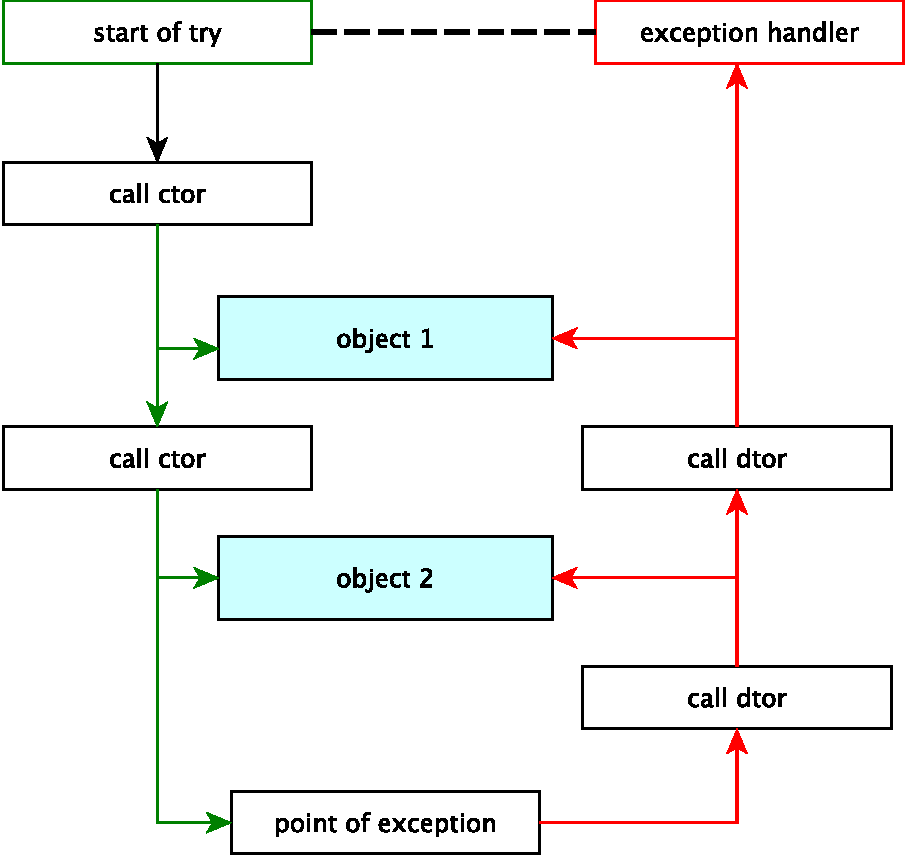
\includegraphics[width=1.0\textwidth]{illustrations/stack-unwind-crop.pdf}
\caption{Stack Unwinding}
\label{fig:stack_unwind}
\end{figure}

Довольно сложно показать на статичном рисунке динамический процесс раскрутки, но идея кажется ясной -- все объекты, созданные от места входа в обработку исключений (пока что можно считать что просто от начала программы) до обработчика удаляются со стека корректно -- то есть с вызовом деструкторов.

\subsubsection{Как правильно поймать исключение}\label{CatchException}

Можно ли обрабатывать исключение самостоятельно? Да, когда дело касается исключений языка C++. Фрагмент кода выражает своё желание обрабатывать исключение с помощью конструкции \lstinline!try!. Результатом \lstinline!throw! является раскрутка стека до тех пор, пока не будет найден подходящий \lstinline!catch!, которому и передаётся управление.

Ниже следует очень плохой пример, так не надо делать никогда:

\begin{lstlisting}
class MathErr {/* ... */};
class Overflow : public MathErr {/* ... */};

void foo()
{
  try {
    /* ... dangerous code here ... */
  }
  catch (MathErr) {
    /* ... dealing with other guys ... */
  }
  catch (Overflow) {
    /* ... dealing with overflow ... */
  }
}
\end{lstlisting}

В приведённом примере исключения перехватываются по значению. Это очень плохо и ведёт к проблеме срезки, рассмотренной в (\ref{Cutting}). Хорошо написанный код перехватывает исключения по константной ссылке или по указателю (если это конечно не исключения POD-типов, которые программист также имеет право возбуждать, их можно перехватывать по значению).

Важно понимать, что обработчики проверяются по порядку перечисления. Поэтому ставить обработчик \lstinline!MathErr! выше чем \lstinline!Overflow!, означает сделать последний чуть более чем бесполезным.

\pagebreak
\subsubsection{Стандартные типы для исключений}\label{ExceptionHierarchy}

Хороший тон это генерировать потомка \lstinline!std::exception! или одного из его потомков в иерархии стандартной библиотеки.

\begin{figure}[h!]
\centering
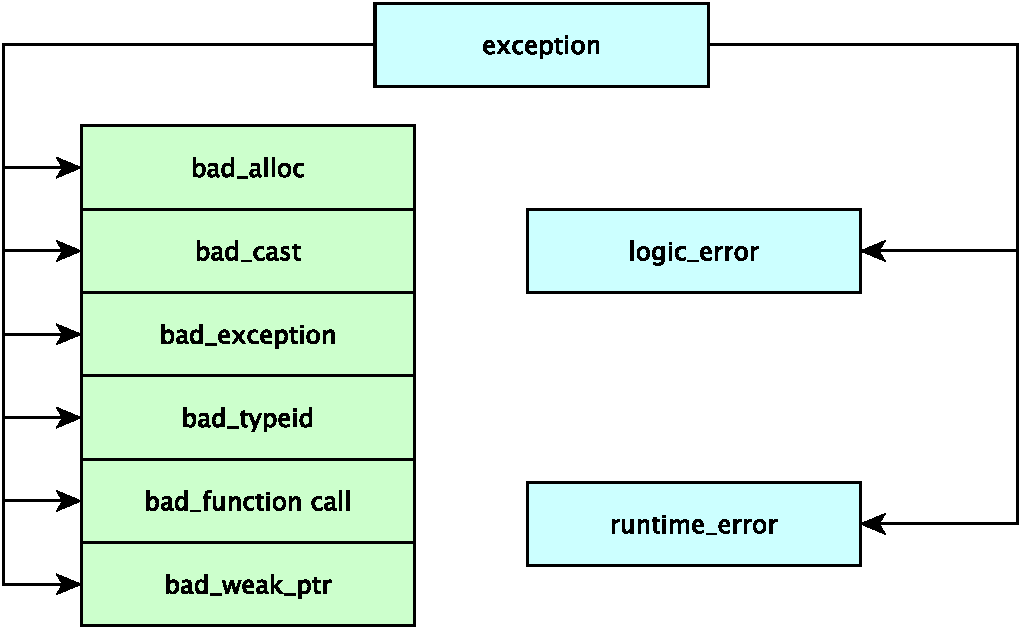
\includegraphics[width=1.0\textwidth]{illustrations/exc-hier-crop.pdf}
\caption{Иерархия стандартных исключений}
\label{fig:exc_hier}
\end{figure}

Слева зелеными обозначены те классы, которые могут быть выброшены в процессе работы со стандартной библиотекой. Справа -- два основных класса, от которых вам предлагается наследовать свои классы-обработчики.

\begin{lstlisting}
class MathErr : public runtime_error {/* ... */};
class Overflow : public MathErr {/* ... */};

void foo()
{
  try {
    /* ... dangerous code here ... */
  }
  catch (const Overflow &) {
    /* ... dealing with overflow ... */
  }
  catch (const MathErr &) {
    /* ... dealing with other guys ... */
  }
}
\end{lstlisting}

Такой вариант кода гораздо более правилен и плюс есть доступ к многочисленным полезным методам этих классов, которые уже там есть.

\subsubsection{Обработка всех возможных исключений}\label{CatchAll}

Опасной, но иногда необходимой конструкцией является перехват всех возможных исключений:

\begin{lstlisting}
void foo()
{
  try {
    /* ... dangerous code here ... */
  }
  catch (...) {
    /* ... dealing with everything??? ... */
  }
}
\end{lstlisting}

Если в вашем коде вы вынуждены использовать такую конструкцию, значит у вас проблемы с проектированием. Единственное исключение -- если вы используете внутри \lstinline!catch (...)! конструкцию перевыброса исключения (\lstinline!throw! без дополнительных аргументов).

\begin{lstlisting}
void foo()
{
  try {
    /* ... critical resource usage here ... */
  }
  catch (...) {
    /* ... cleaning up critical resource ... */
    throw; /* and rethrow */
  }
}
\end{lstlisting}

Перевыброшенное исключение продолжит размотку стека пока не будет поймано кем-то, кто знает как его обработать. Если выброшенное исключение не нашло своего обработчика, оно инициирует вызов функции \lstinline!terminate! и аварийный выход из программы. Кроме перевыброса того же исключения (\lstinline!throw! без параметра, которое может встретиться только внутри \lstinline!catch!-блока) вы можете в любом месте использовать \lstinline!throw! с параметром, для того чтобы бросить произвольное исключение. 

Вообще освобождение ресурсов с помощью деструкторов предпочтительней использования для этой цели \lstinline!try!-блоков с перехватом всех исключений.

Иногда перехват всевозможных исключений срабатывает неожиданно

\begin{lstlisting}
struct my_exc1 : std::exception { 
    char const* what() const throw(); 
};

struct my_exc2 : std::exception { 
    char const* what() const throw(); 
};

struct your_exc3 : my_exc1, my_exc2 {};

int main()
{
   try { throw your_exc3(); }
   catch(std::exception const& e) {}
   catch(...) { printf("whoops!\n"); }
}
\end{lstlisting}

\textbf{Вопрос к студентам:} как избежать здесь whoops?

\ifanswers
Правильный ответ: виртуальное наследование.
\fi

\pagebreak
\subsection{Вопросы безопасности исключений}\label{ExceptionSafety}

Исключения, являясь частным случаем нелокальной управляющей конструкции, добавляют строчки в неявный контракт на каждый метод и добавляют неожиданные дуги возможного выхода в каждом месте вызова небезопасной с точки зрения генерации исключений функции. Поэтому при проектировании кода, серьёзно использующего исключения, программист несёт дополнительную интеллектуальную нагрузку. Он должен следить за тем, что называется безопасностью кода относительно исключений.

\subsubsection{Гарантии безопасности исключений\index{Exception Safety Guarantees}}\label{SafetyGuarantees}

Существует три гарантии безопасности, которые может предоставлять код:

\begin{itemize}
\item
\textbf{Базовая гарантия} заключается в том, что сбой при выполнении операции может изменить состояние программы, но не вызывает утечек и оставляет все объекты в согласованном (но не обязательно предсказуемом) состоянии, т.е. пригодными к дальнейшему использованию.
\item
\textbf{Строгая гарантия} обеспечивает транзакционную семантику: при сбое операции гарантируется неизменность состояния программы относительно задействованных в операции объектов.
\item
\textbf{Гарантия бессбойности} означает, что функция не генерирует исключений.
\end{itemize}

При написании кода на C++ следует придерживаться хотя бы одной из этих гарантий и предпочитать идиому RAII, которая рассматривалась в (\ref{RAII}). Также исключения не должны генерироваться деструкторами, функциями, освобождающими ресурсы и функциями обмена.

\subsubsection{Безопасное копирование}\label{SafeCopying}

Вернемся к шаблонному классу стека и теперь попытаемся сделать его безопасным относительно исключений, в целом следуя изложению в \cite{exceptionalcpp}. На первый взгляд, интерфейс стека может выглядеть как-то вот таким образом:

\begin{lstlisting}
template <typename T> 
class Stack
{
public:
  Stack(): m_v(new T[10]), m_vsize(10), m_vused(0) {}
  ~Stack() { delete [] v; }
  Stack(const Stack&);
  Stack& operator= (const Stack&);
  void Push(const T&);
  T Pop();
private:
  T* m_v;
  size_t m_vsize;
  size_t m_vused;
};
\end{lstlisting}

Конструктор и деструктор уже тривиально безопасны (если исключения не выходят за \lstinline!delete[]!, но они и не должны за него выходить). Сложнее с копированием и копирующим присваиванием. Проще всего сделать безопасным копирующий конструктор, определив шаблон общей вспомогательной функции \lstinline!safe_copy!, копирующей буфер в заданный с перехватом всех возможных исключений и освобождением ресурсов.

\begin{lstlisting}
template <typename T>
T *safe_copy(const T* src, size_t srcsize, size_t destsize)
{
  size_t idx;
  T * dest;
  assert (destsize >= srcsize);
  dest = new T[destsize];
  try 
    {
       for (idx = 0; idx != srcsize, ++idx)
         dest[idx] = src[idx];
    }
  catch (...)
    {
       delete [] dest;
       throw;
    }
  return dest;
}
\end{lstlisting}

\textbf{Вопрос к студентам:} почему цикл, а не не \lstinline!memcpy!?

\ifanswers
Правильный ответ: потому что должны быть вызваны операторы присваивания для \lstinline!T!.
\fi

\textbf{Вопрос к студентам:} где в этой функции могут быть сгенерированы исключения?

\ifanswers
Внутри этой функции исключения могут быть сгенерированы:

\begin{itemize}
\item
В функции \lstinline!new!, переопределённым для \lstinline!T! оператором \lstinline!operator new! или конструктором  \lstinline!T! -- в этом случае никакой памяти выделено не будет и утечки не произойдёт, а исключения покинут  \lstinline!safe_copy!
\item
В функции  \lstinline!operator=! или  \lstinline!operator[]! типа  \lstinline!T! при копировании. В этом случае исключения будут перехвачены, ресурсы освобождены и исключения отпущены дальше.
\end{itemize}
\fi

Имея эту функцию, уже можно разработать симпатичный конструктор копирования

\begin{lstlisting}
template <typename T>
Stack<T>::Stack(const Stack& rhs) : 
    m_v(safe_copy(rhs.m_v, rhs.m_vsize, rhs.m_vsize)),
    m_vsize(rhs.m_vsize), 
    m_vused(rhs.m_vused) 
{
}
\end{lstlisting}

Единственный источник исключений здесь -- \lstinline!safe_copy!, в которой никакой утечки быть не может. Общий урок раздела заключается в том, что все места, где может быть сгенерировано исключение полезно собрать в одну вспомогательную функцию для использования безопасным образом.

\subsubsection{Безопасное присваивание и copy-and-swap idiom}\label{CopySwap}

Теперь присваивание. Саттер рекомендует сделать присваивание следующим образом:

\begin{lstlisting}
template <typename T>
Stack<T>& Stack<T>::operator=(const Stack<T>& rhs)
{
  T *v_new;

  if (this == &rhs)
    return *this;

  v_new = safe_copy(rhs.m_v, rhs.m_vsize, rhs.m_vsize);
  delete [] m_v;
  m_v = v_new;
  m_vsize = rhs.m_vsize; 
  m_vused = rhs.m_vused;
  return *this;
}
\end{lstlisting}

Таким образом состояние остаётся неизменным и даже при генерации исключения, оно выходит наружу не нарушая консистентности объекта.

Но этот подход кажется несколько избыточным. Вместо него можно воспользоваться уже имеющимся конструктором копирования.

\begin{lstlisting}
/* Copy ctor reused on argument construction! */
template <typename T>
Stack<T>& Stack<T>::operator=(const Stack<T> rhs)
{
  std::swap (rhs.m_v, this->m_v);
  std::swap (rhs.m_vsize, this->m_vsize);
  std::swap (rhs.m_vused, this->m_vused);
}
\end{lstlisting}

Здесь \lstinline!swap! это обмен значениями из стандартной библиотеки (он никогда не кидает исключений т.к. работает с примитивными типами). Можно думать об этой функции как о стандартном варианте:

\begin{lstlisting}
template <typename T>
void swap(T& a, T& b)
{
  T temp(a);
  a = b;
  b = temp;
}
\end{lstlisting}

Но не стоит реализовать его таким образом самостоятельно, пока что лучше взять стандартный. В последующих лекциях будут рассмотрены гораздо лучшие варианты реализации обмена с помощью rvalue references.

Можно написать метод \lstinline!Stack<T>::swap! и тогда код присваивания упростится до одной строчки.

Этот подход называется copy-and-swap идиомой и содержит важный урок -- переиспользование кода не только облегчает его написание и понимание, но и помогает обеспечить безопасность исключений для этого кода.

\textbf{Домашняя наработка:} реализовать безопасное помещение в стек. Можно ли переиспользовать \lstinline!swap! или \lstinline!safe_copy!?

\subsubsection{Неявное копирование и безопасность исключений}\label{ImplicitCopy}

Проблемы, как обычно, подстерегают там, где их не ждали. Давайте рассмотрим метод \lstinline!Pop()!, который пока что остался не реализованным. К сожалению, его реализация только кажется простой.

\begin{lstlisting}
template <typename T>
T Stack<T>::Pop(void)
{
  T result;

  assert(m_vused > 0);
  result = m_v[m_vused - 1];
  m_vused -= 1;
  return result;
}
\end{lstlisting}

Вся проблема с этим кодом заключается в его возможном использовании:

\begin{lstlisting}
Stack<Sometype> s;
SomeType s2;
/* .. some code .. */
s2 = s.Pop();
\end{lstlisting}

В последней строчке происходит копирование возвращаемого \lstinline!SomeType! в место назначения. Если в этот момент возникнет исключение, то все побочные эффекты со стеком уже окажутся учтены -- элемент будет снят с верхушки, но он пропадёт безвозвратно. Именно поэтому в коде стандартной библиотеки и в любом безопасном относительно исключений коде, эти операции разделены:

\begin{lstlisting}
template <typename T> 
class Stack
{
public:
  Stack(): m_v(new T[10]), m_vsize(10), m_vused(10) {}
  ~Stack() { delete [] v; }
  Stack(const Stack&);
  Stack& operator= (const Stack&);
  void Push(const T&);
  T& Top();
  void Pop();
private:
  T* m_v;
  size_t m_vsize;
  size_t m_vused;
};
\end{lstlisting}

Метод \lstinline!Top()! даёт верхний элемент но не модифицирует стек, метод \lstinline!Pop()! модифицирует стек но не возвращает никакого значения, безопасность исключений соблюдена. Основной урок здесь состоит в том, что безопасность исключений действительно влияет на проектирование класса и думать о ней необходимо уже на этапе проектирования.

\subsubsection{Идиома PImpl\index{PImpl} для безопасного кода}\label{PImpl}

В \cite{exceptionalcpp} предложена элегантная идиома для написания безопасного относительно исключений кода -- \textbf{Pointer to Implementation} или сокращённо PImpl. Поскольку проблемы утечки ресурсов вызваны работой с ресурсами (в данном случае -- с памятью), эту работу можно инкапсулировать в специальный класс с изящным интерфейсом. Сначала необходимо написать две вспомогательные функции. Первая \lstinline!destroy! вызывает деструктор объекта, не освобождая его память

\begin{lstlisting}
template <class T> void
destroy(T* p)
{
  p->~T();
}
\end{lstlisting}

Вторая \lstinline!construct! создает объект в существующей памяти через placement new, который был рассмотрен в (\ref{PlacementNew}) (тут можно позвать кого-нибудь написать у доски).

\begin{lstlisting}
template <class T1, class T2> void
construct (T1 *p, const T2 &value)
{
  new (p) T1 (value);
}
\end{lstlisting}

И далее -- более сложная функция \lstinline!destroy! уничтожает содержимое обобщённого forward-итерируемого контейнера:

\begin{lstlisting}
template <typename FwdIter>
void destroy( FwdIter first, FwdIter last )
{
  while ( first != last )
    {
      destroy( &*first ); 
      ++first;
    }
}
\end{lstlisting}

Теперь код, прячущий за своим фасадом работу с ресурсами типа T, может быть реализован в терминах этих обобщённых функций:

\begin{lstlisting}
template <typename T>
class StackImpl
{
  StackImpl(const StackImpl &);
  StackImpl& operator= (const StackImpl &);

protected:
  StackImpl(size_t size = 0): 
      m_v(operator new (sizeof(T) * size)), 
      m_vsize(size), 
      m_vused {
  }

  ~StackImpl() { 
    destroy(m_v, m_v + m_vused); 
    ::operator delete(m_v); 
  }

  void Swap(StackImpl<T> &other) {
    swap( m_v, other.m_v );
    swap( m_vsize, other.m_vsize );
    swap( m_vused, other.m_vused );
  }
  T *m_v;
  size_t m_vsize, m_vused;
};
\end{lstlisting}

Используя этот класс, можно реализовать приватно наследующий от него стек

\begin{lstlisting}
template<typename T> 
struct Stack : private StackImpl<T>
{
  Stack( size_t size = 0 ) : StackImpl<T>(size) {}
  Stack( const Stack& other ) : StackImpl<T>(other.m_vused)
  {
    while( m_vused < other.m_vused )
      {
        construct (m_v + m_vused, other.m_v[m_vused]);
        m_vused += 1;
      }
  }

  Stack<T>& operator = (const Stack<T>& other)
  {
    Stack tmp(other);
    this->stack_swap(tmp);
    return *this;
  }
 
  size_t count() const { return m_vused; }

  void push( const T& value )
  {
    if( m_vused == m_vsize )
      {
        Stack tmp(2*m_vsize + 1);
        while (tmp.count() < m_vused)
          tmp.push (m_v[tmp.count()]);

        tmp.push (value);
        this->stack_swap (tmp);
      }
    else
      {
        construct( m_v + m_vused, value );
        ++m_vused;
      }
  }

  T& top() {return m_v[m_vused - 1];}

  void pop()
  {
    --m_vused;
    destroy (m_v + m_vused);
  }
};
\end{lstlisting}

Он удовлетворяет гарантии бессбойности -- самой строгой из трёх гарантий Абрамса -- ни одна из его функций не генерирует исключений и безопасна.

\subsubsection{Что нельзя деструкторам и можно нам}\label{ExcDestructors}

В предыдущем разделе функция \lstinline!destroy! могла вызвать обоснованную критику: она очевидно не защищена от ситуации когда деструктор уничтожаемого объекта выбрасывает исключение. Программист мог бы попробовать переписать её в защищённом стиле:

\begin{lstlisting}
template <typename FwdIter>
void destroy( FwdIter first, FwdIter last )
{
  while ( first != last )
    {
      try 
        {
          destroy( &*first ); 
        }
      catch (...)
        {
          /* what to do here? */
        }
      ++first;
    }
}
\end{lstlisting}

Основная проблема -- что делать в обработчике. Есть три идеи и все три очень плохи.
\begin{enumerate}
\item
Можно снова генерировать в обработчике перехваченное исключение. Тогда функция удовлетворяет гарантии нейтральности... и, пожалуй, всё. При этом destroy не сможет сообщить о количестве корректно уничтоженных объектов и не уничтоженные останутся не уничтоженными, что вызовет утечку ресурсов
\item
Можно, перехватывая исключение, генерировать некое другое исключение. Тогда функция не удовлетворяет гарантии нейтральности и всё равно может вызвать утечку
\item
Можно, перехватывая исключения, как-то гасить их (может быть с некоторой обработкой). Но тогда функция не удовлетворяет гарантии нейтральности и, с точки зрения вызывающей функции, скрывает ошибки
\end{enumerate}

Итак, если деструктор \lstinline!T! может генерировать исключения, всё сведётся к написанию в лучшем случае небезопасного кода. Этой проблеме также подвержены невинно выглядящие \lstinline!new[]! и \lstinline!delete[]!, о которых шла речь в (\ref{newdelete}).

\begin{lstlisting}
T *arr = new T[10];
delete [] arr;
\end{lstlisting}

\textbf{Вопрос к студентам:} как будет вести себя этот код, если предположить, что деструктор \lstinline!T! может генерировать исключения?

\ifanswers
TODO: здесь правильный и обоснованный ответ
\fi

Вывод из этого довольно прост: никогда не пишите типы, деструкторы которых, могут сгенерировать исключения. Гораздо сложнее тема с генерацией исключений конструкторами, но её я склонен оставить на самостоятельное изучение по \cite{exceptionalcpp}

\pagebreak
\subsection{Исключения под капотом\index{setjmp}\index{longjmp}}\label{Longjmps}

Для того, чтобы лучше понимать исключения, бывает полезно попробовать реализовать их руками (как это было сделано с виртуальными функциями ранее). Пример заменяет тысячу слов. Допустим функция \lstinline!allocate! вызывает \lstinline!malloc! чтобы выделить n байт, и возвращает указатель, который вернул \lstinline!malloc!. Если же \lstinline!malloc! возвращает нулевой указатель, что индицирует нехватку памяти, \lstinline!allocate! делает нечто похожее на возбуждение исключения \lstinline!Allocate_Failed! (без размотки стека и вызова деструкторов пока что). Исключение само по себе имеет тип \lstinline!jmp_buf!, который определён в стандартном хедере \lstinline!setjmp.h!:

\begin{lstlisting}
#include <setjmp.h>

int Allocation_handled = 0;
jmp_buf Allocate_Failed;
\end{lstlisting}

\lstinline!Allocation_handled! ноль, пока обработчик не инстанциирован и \lstinline!allocate! проверяет \lstinline!Allocation_handled! прежде чем возбуждать исключение:

\begin{lstlisting}
void *allocate(unsigned n) {
  void *new = malloc(n);
  if (new)
    return new;
  if (Allocation_handled)
    longjmp(Allocate_Failed, 1);
  assert(0);
}
\end{lstlisting}

И теперь можно сделать практически \lstinline!try! и \lstinline!catch!:

\begin{lstlisting}
/* try { */
Allocation_handled = 1;
if (setjmp(Allocate_Failed)) {
  goto alloc_except_label;
}

/* ... here some code, calling somewhere allocate() */

/* } */
/* catch (...) { */
alloc_except_label:
/* ... here processing exception */
Allocation_handled = 0;
/* } */
\end{lstlisting}

Осталось добавить раскрутку стека и прочий сахар, который насыпан для этого в C++, но идея должна быть уже понятна.

\pagebreak
\subsection{Домашняя наработка по исключениям}

\textbf{Контрольные вопросы}

\begin{enumerate}
\item В чем разница между локальными и нелокальными управляющими конструкциями?
\item Что является и что не является исключительной ситуацией в терминах C++?
\item Чем неконсистентное состояние объекта отличается от неопределенного? Приведите пример.
\item Может ли при размотке стека после исключения возникнуть висячая (dangling) ссылка? Приведите пример.
\item У вас есть выбор -- ловить исключение по ссылке или по указателю. Какие аргументы за и против вы приведете и что выберете?
\item Что произойдет если при создании объекта исключения, его конструктор выбросил исключение?
\item Можно ли бросить и поймать объект исключения с запрещенным копированием и перемещением? А перевыбросить?
\item В списке инициализации конструктора два указателя инициализируются через new. Как обеспечить чтобы оба были либо полностью выделены либо освобождены и конструирование всего объекта выбросило исключение?
\item По ссылкам на каких предков (левого, правого или общего) можно поймать в обработчике исключения объект самого нижнего производного класса при ромбовидном наследовании?
\item Какие гарантии безопасности исключений вам известны? Приведите примеры.
\item Можно ли для класса с динамическим выделением одного из полей как-то гарантировать, что исключения не покинут копирующий конструктор?
\item Copy and swap idiom -- что это такое, применимость, примеры
\item Почему в стандартной библиотеке метод \lstinline!vector<T>::pop_back()! не возвращает значение удаленного из вектора элемента? (Подсказка: это как-то связано с безопасностью относительно исключений).
\item Как расшифровывается PImpl и зачем нужна эта идиома?
\item Исходя из чего разработчики языка решили, что исключение в деструкторе всегда приводит к аварийному завершению программы?
\item Что происходит если исключение покидает конструктор?
\end{enumerate}

\textbf{Задачи}

\begin{enumerate}

\item Разработайте безопасный относительно исключений шаблон \lstinline!Vector<T>! на основе идиомы PImpl. Функция \lstinline!push_back! или её аналог должна сообщать о нехватке памяти, выбрасывая исключение.

\item Предложите и реализуйте набор тестов для шаблона \lstinline!Stack<T>! для того, чтобы убедиться, что он поддерживает строгую транзакционную семантику.

\item Оцените где могут возникнуть исключения в следующем коде? Является ли он безопасным относительно исключений?

\begin{lstlisting}
std::vector <T>
bitvise_or (std::vector <T> a, std::vector <T> b)
{
  if ((a.size () == 0) || (b.size () == 0))
    std::cout << "Nothing to or with" << std::endl;
  else if (a.size () != b.size ())
    std::cout << "Can not process arrays of inequal size" 
              << std::endl;
  else if (a.size () > 10)
    std::cout << "Arrays too large" << std::endl;
  else
    {
      std::vector <T> ret (a.size ());
      for (auto i = a.begin(), 
                j = b.begin(), 
                k = ret.begin();
           i != a.end (); 
           i++, j++, k++)
        *k = *i | *j;
      return ret;
    }
}
\end{lstlisting}

Предложите как его улучшить.

\end{enumerate}

\pagebreak
\section{Лабиринты стандартной библиотеки}

\hfill\textit{Most software today is very much like an Egyptian pyramid}

\hfill\textit{with millions of bricks piled on top of each other,}

\hfill\textit{with no structural integrity,}

\hfill\textit{but just done by brute force and thousands of slaves}{\vspace{0.5em}}

\hfill\textit{-- Alan Kay}

Стандартная библиотека языка C++ имеет долгую и интересную историю. Идея стандартизировать библиотеку в языке C (из которой позже выросла стандартная библиотека C++) возникла не сразу. Первая стандартизация библиотеки языка C это стандарт ANSI C 1989-го и последовавший за ним ISO/IEC 9899-1990 \cite{stdc90}. Эта библиотека известна под названиями libc или crt (от C run-time support) и часто модифицировалась и подвергалась изменениям и расширениям. Стандартная библиотека C++-98, включает стандартную библиотеку C по нормативной ссылке, добавляя к ней свои части, известные ранее под общим названием STL и расширенные (и постоянно расширяемые в новых стандартах) комитетом по стандартизации.

Идея что включать и что не включать в стандартную библиотеку языка программирования не так тривиальна, как может показаться: 
\begin{itemize}
\item
Некоторые языки поставляются с библиотеками включающими всё, что может понадобиться когда бы то ни было, включая крайне высокоуровневые функции работы с XML, базами данных, сетевыми протоколами. Это философия таких языков как Python, Java, C\#, которые идут ``с батарейками внутри''.
\item
Стандартная библиотека языка С (и некоторых других) придерживается, наоборот, философии минимальной поддержки, включая только те функции, которые могут пригодиться каждому разработчику (и некоторые функции, которые вызвали слезы няшного умиления у комитета стандартизации и оставлены, хотя не нужны, пожалуй, вообще никому, например strcspn).
\item
Язык C++ занимает промежуточную позицию. По своей задумке его библиотека придерживается второго подхода, но по факту от стандарта к стандарту асимптотически сходится к первому.
\end{itemize}

Этот раздел посвящен рассмотрению стандартной библиотеки C++ как составного, ``двуединого'' целого из унаследованной стандартной библиотеки C и добавленных к ней средств, таких, как шаблонные контейнеры, итераторы, алгоритмы, потоковый ввод и вывод и так далее. При этом две её части находятся в диалектическом конфликте (знакомом каждому, кто хоть раз пробовал смешивать их средства), но и в диалектическом единстве взаимной поддержки.

\subsection{Строки}

Несмотря на то, что с первого взгляда строка это просто вектор символов, работа со строками исторически всегда выделялась в отдельные функции. В языке C начиная с самых ранних вариантов были специальные средства для работы с ``C-строками'' -- последовательностями \lstinline!char!, с нулевым символом в качестве признака конца. Они общеизвестны и не знать что делают такие функции как \lstinline!strlen!, \lstinline!strcpy! или, например, \lstinline!strcat! недопустимо.

\textbf{Вопрос к студентам:} что делает \lstinline!strcat!?

\ifanswers
Правильный ответ: дописывает в конец строки, на начало которой указывает первый аргумент, строку, на начало которой указывает второй аргумент. При этом первый символ второй строки замещает завершающий нулевой символ первой
\fi

\textbf{Вопрос к студентам:} верно ли утверждение 

\lstinline!strlen(strcat(x, y)) == strlen(x) + strlen(y)! 

для всех C-строк \lstinline!x! и \lstinline!y!?

\ifanswers
Правильный ответ: да, потому что \lstinline!strlen! не учитывает завершающий нуль
\fi

\textbf{Вопрос к студентам:} как насчет \lstinline!strcspn!?

\ifanswers
Правильный ответ: вычисляет длину максимального начального сегмента первого аргумента не содержащего ни одного символа из второго аргумента. Знать это вовсе не обязательно. За пример полезного использования этой функции автор был бы признателен.
\fi

Работа с C-строками имеет свои привлекательные стороны, но такие строки не являются объектами первого класса в языке, а также работа с ними часто подвержена порче памяти и выходу за границы. Ещё сложнее ситуация становится с появляением разных кодировок, например для поддержки Unicode. Подумайте на секундочку о функции \lstinline!wcscspn!.

При этом сама концепция C-строки в принципе уникальна среди языков программирования. Обычный подход -- заставлять строки в явном виде хранить свою длину и делать их первоклассными объектами.

С ранних версий стандарта C++ перед разработчиками стояла задача -- сохранить эффективность C-строк и совместимость с ними и одновременно сделать нормальные строки для использования вне критичных для производительности контекстов.

\subsubsection{От обработки строк в стиле C к C++}\label{CStringToStdString}

Стандартная библиотека языка C и все её возможности по ссылке включены в стандарт C++ и могут использоваться, как обычно. Но добавленный также класс \lstinline!basic_string! и его специализации \lstinline!string! и \lstinline!wstring! позволяют делать то же самое гораздо безопаснее и во многом проще (иногда ценой производительности).

Каноническая задача -- заменить в строке все подстроки данного вида. Скажем в строке \lstinline!"Hello, $username, how are you doing, $username?"! заменить все вхождения \lstinline!$username! на \lstinline!Eric, the Bloody Axe!.

\textbf{Задача у доски:} написать это на C++ без \lstinline!std::string!.

Задача непроста и требует некоторого размышления. Между тем на современном C++ она решается очень просто (даже не используя алгоритмов стандартной библиотеки, просто с помощью встроенных средств типа \lstinline!string!)

\begin{lstlisting}
void
replace_all (std::string& str,
             const std::string& from,
             const std::string& to)
{
  size_t start_pos = 0;

  if (from.empty ())
    return;

  while ((start_pos = str.find (from, start_pos)) != std::string::npos)
    {
      str.replace (start_pos, from.length(), to);

      // In case 'to' contains 'from', like replacing 'x' with 'yx'
      start_pos += to.length(); 
    }
}
\end{lstlisting}

Как использовать эту функцию?

\begin{lstlisting}
int
main (void)
{
  std::string str = "Hello, $username, how are you doing, $username?";
  std::string from = "$username";
  std::string to = "Eric, the Bloody Axe";

  replace_all (str, from, to);

  std::fprintf (stdout, "%s\n", str.c_str());

  return 0;
}
\end{lstlisting}

Обратите особое внимание на метод \lstinline!c_str()!, позволяющий получить C-строку для использования в функциях, где нужно C API (скажем \lstinline!fprintf!).

Вариант в более C++ стиле (см. \ref{PrintfToCout}) будет также проще в записи:

\begin{lstlisting}
cout << str << endl;
\end{lstlisting}

Конечно, вариант с C-строками можно написать так, что он выиграет у варианта с C++ строками представленного выше, но только на экстремально длинных строках, которые, в общем, редкость. Но да, в любом случае это надо учитывать. Автору приходилось убирать perf issues из кода, который занимался копированием сотен тысяч небольших строк через оператор присваивания класса \lstinline!std::string!.

\subsubsection{Строки народов мира}

Не все буквы можно поместить в диапазон однобайтных символов. Пока речь идёт только об английском языке, всё неплохо, но русские буквы, европейская диакритика, и даже иероглифическое письмо также имеют свое место в мире C++.

TODO: требует написания

Скорее всего стоит читать эту часть вне обязательного курса, по желанию.
Тут про то что студентам нужно знать о Unicode, а также про \lstinline!wstring! 

Дополнительно упомянуть \lstinline!u16string! и \lstinline!u32string! из нового стандарта.
Дополнительно locale и strcoll.

\pagebreak
\subsection{Случайные числа}\label{RandomNumbers}

Здесь описание хедера \lstinline!<random>!

\pagebreak
\subsection{Время}\label{Chrono}

Здесь описание хедера \lstinline!<chrono>!

\pagebreak
\subsection{Последовательные контейнеры}\label{SeqContainers}

\hfill\textit{Good surgeon knows when not to cut}

\hfill\textit{Good programmer should know when not to code}{\vspace{0.5em}}

\hfill\textit{-- Walter Brown}

Контейнеры STL отражают абстракцию структур данных. Все практически важные структуры уже представлены или могут быть представлены контейнерами. Наиболее известны следующие последовательные контейнеры:

\begin{itemize}
\item \textbf{vector} -- массив с гарантиями непрерывной области памяти и динамическим ростом с одной стороны
\item \textbf{deque} -- массив со странично организованной памятью и ростом с двух сторон.
\item \textbf{list} -- двусвязный список с быстрой вставкой и удалением элементов
\item \textbf{forward\_list} -- односвязный список с быстрой вставкой и удалением элементов
\item \textbf{array} -- массив с фиксированным на этапе компиляции размером
\end{itemize}

Кроме них существуют также ассоциативные контейнеры, которые будут рассмотрены в (\ref{AssociativeContainers}).

\subsubsection{Стандартные операции над контейнерами}\label{StandardOperations}

Все контейнеры STL поддерживают общие операции: \lstinline!size()!, \lstinline!empty()!, \lstinline!max_size()!, операторы сравнения, \lstinline!swap()!, \lstinline!begin()!, \lstinline!end()!, \lstinline!rbegin()!, \lstinline!rend()!, \lstinline!insert()!, \lstinline!erase()!, \lstinline!clear()! и некоторые другие, которые в совокупности можно считать шаблонным интерфейсом, имплементируя который любой класс так же может называться контейнером STL.

Любой контейнер содержит конструктор по умолчанию, копирующий конструктор и открытый невиртуальный деструктор. Последнее крайне важно. Стандарт, нормы коммьюнити, а иногда даже и сообщения компилятора прямо и недвусмысленно \textbf{запрещают} наследование от шаблонных контейнеров стандартной библиотеки. Как мы помним из \ref{VirtDestr}, наличие невиртуального деструктора в классе -- достаточное основание никогда ничего от него не наследовать.

\subsubsection{Требования к элементам контейнеров STL}\label{STLReqs}

Контейнеры STL являются шаблонами, а все шаблонные интерфейсы являются неявными. Поэтому программист должен хорошо знать неявные требования, предъявляемые к элементам контейнеров, как к чему-то, что может быть помещено в данный контейнер.

\begin{itemize}
\item \textbf{Копируемость} -- у объекта должен быть определён стандартный или пользовательский копирующий конструктор, который должен действительно копировать объект
\item \textbf{Изменяемость} -- объект должен быть lvalue с действительным оператором присваивания
\item \textbf{Конструируемость} -- хотя бы один из конструкторов и хотя бы один из деструкторов объекта должны быть открытыми
\end{itemize}

Некоторые контейнеры определяют дополнительные неявные требования, такие как наличие критерия сортировки (для упорядоченных конструкций) или конструктора по умолчанию.

\subsubsection{От встроенных массивов к векторам}\label{vectorarrs}

Одной из главных проблем, которые красной нитью проходили через все лекции была проблема управления памятью. Правильно спаривать \lstinline!new! и \lstinline!delete!, использовать RAII для управления ресурсами, управлять памятью в безопасном для исключений стиле -- всё это важные и нужные навыки. Но внутри стандартной библиотеки содержится контейнер, который для большинства практических случаев позволяет в принципе избегать явного использования динамической памяти. Это класс \lstinline!vector!. Он определён в заголовке \lstinline!<vector>! стандартной библиотеки как:

\begin{lstlisting}
template <typename T, typename Allocator = allocator<T> >
class vector;
\end{lstlisting}

Таким образом вместо

\begin{lstlisting}
int *n = new int[10];
n[5] = 5;
\end{lstlisting}

Можно писать

\begin{lstlisting}
std::vector<int> n(10);
n[5] = 5;
\end{lstlisting}

Для достижения такого эффекта, вектор использует переопределение оператора квадратных скобок. Это похоже на переопределение оператора круглых скобок, рассмотренное ранее.

Вектора в C++ также поддерживают операцию \lstinline!push_back!, для динамического роста. К сожалению, это убивает детерминированность в работе вектора с памятью, поэтому аккуратный программист всегда использует резервирование памяти для того, чтобы исключить перераспределение при добавлении пары элементов

\begin{lstlisting}
std::vector<int> n;
n.reserve(80); /* place for 80 ints */
\end{lstlisting}

Но зарезервированное место ещё не распределено, поэтому вызывать квадратные скобки можно только с реальным индексом -- не превосходящим \lstinline!n.size()!.

Использовать вектор всегда предпочтительней, чем работать с массивами напрямую. Следующий пример представляет собой не слишком безопасный относительно исключений код:

\begin{lstlisting}
template <typename T>
T foo (int n)
{
  T *t = new T[n], ret = 0;

  init_t (t, n); // exc!
  
  for (int i = 0; i < n; ++i)
    {
      if (!check_legal(t[i])) // exc!
        {
          delete [] t;
          throw std::runtime_error("Illegal element");
        }

      ret += t[i]; // exc!
    }

  delete [] t;

  return ret;
}
\end{lstlisting}

Он изобилует проблемами и местами, где возможна утечка. К тому же его элементарно сложно читать. Давайте посмотрим как этот код магически трансформируется в нечто гораздо более прозрачное и безопасное.

\begin{lstlisting}
template <typename T>
T foo (int n)
{
  std::vector<T> t(n);
  T ret = 0;

  /* legal! vector in memory laid out continously */
  init_t (&t[0], n); 

  size_t vsz = t.size();
  for (int i = 0; i != vsz; ++i)
    {
      if (!check_legal(t[i]))
        throw std::runtime_error("Illegal element");

      ret += t[i];
    }

  return ret;
}
\end{lstlisting}

При выбросе исключения, память под вектором будет корректно освобождена. Впрочем, тут ещё есть, что улучшать. Когда разговор зайдёт про итераторы и алгоритмы, это будет сделано и вы увидите космос.

\subsubsection{Списки и деки}

В разделе (\ref{vectorarrs}) был продемонстрирован пример, который не следует недооценивать. Итак, есть функция \lstinline!init!, ожидающая указателя на непрерывную область данных

\begin{lstlisting}
template <typename T>
void init (T*, int);
\end{lstlisting}

Легально передать туда указатель на первый элемент вектора:

\begin{lstlisting}
std::vector<T> t(n);

/* legal! vector in memory laid out continously */
init_t (&t[0], n);
\end{lstlisting}

Это очень строгая гарантия. На самом деле, последовательный контейнер может быть устроен так, чтобы не обязательно её давать -- например занимать произвольные участки памяти. Например это позволило бы сделать в таком контейнере эффективный \lstinline!push_front!, \lstinline!insert! или \lstinline!emplace! после любого элемента и так далее. Для таких целей, библиотека поддерживает односвязные списки (\lstinline!std::forward_list!), двусвязные списки (\lstinline!std::list!) и деки (\lstinline!std::deque!).

Односвязные и двусвязные списки в комментариях не нуждаются. Их главная проблема -- так себе амортизированное время доступа к элементу, главное достоинство -- вставка за O(1) в любую позицию. Гораздо интереснее деки.

Дека это почти магический контейнер, который поддерживает:

\begin{itemize}
\item Доступ к любому элементу за O(1) 
\item Вставку в начало и в конец за O(1) 
\item Вставку в произвольное место за O(n)
\end{itemize}

\textbf{Вопрос к студентам:} как бы вы организовали такой контейнер?

\ifanswers
Правильный ответ: последовательность кусков памяти фиксированного размера, связанных в цепочку
\fi

\subsubsection{Вектор булевых значений}

Самое плохое в \lstinline!vector<bool>!, что он не \lstinline!vector! и что он не хранит \lstinline!bool!.

Интенция при этом была хорошей. \lstinline!vector<bool>! — это специализация шаблона \lstinline!vector!, компактно хранящая данные, выделяя по одному биту на каждый булев признак, а не по одному байту, который традиционно занимает тип \lstinline!bool!.

Увы, с таким подходом этот контейнер не хранит \lstinline!bool!, потому что при индексации такой вектор не может вернуть ссылку на \lstinline!bool!. По сути ему нужно каким-то образом вернуть ссылку на один бит. В результате приходится использовать \lstinline!vector<bool>::reference! — некий проксирующий тип, который пытается имитировать своим поведением ссылку на \lstinline!bool!.

И кроме того, с таким подходом он не является вектором, так как не удовлетворяет требованиям к контейнеру \lstinline!vector! по линейной организации памяти:

\begin{lstlisting}
std::vector<T> t(n);
/* illegal only if T is bool */
bool *b = &t[0];
assert (b[1] == t[1]);
\end{lstlisting}

В этом случае следующий за первым при инкременте указателя элемент вовсе не является тем элементом, который реально хранится на соответствующей позиции в контейнере.

Пример с вектором булевых значений крайне поучителен: при проектировании обобщенного кода такого рода специализации вредны. Лучше было бы сделать отдельный класс, такой как \lstinline!std::bitvector!.

\subsubsection{От векторов обратно к массивам}

Вектор -- хорошая вещь, но объективно он тяжеловесен, а возможность динамически его переаллоцировать не всегда нужна. Все разработчики годами жили с C-style arrays. Начиная с 11-го года в C++ поддерживается стандартный контейнер \lstinline!std::array! -- максимально легковесное приближение к встроенному массиву. Размер такого массива задается на этапе компиляции и не может быть изменен, но при этом все операции с ним так же просты, как и с прочими контейнерами стандартной библиотеки.

Основные отличия таких массивов от встроенных перечислены ниже

\begin{enumerate}

\item
Они не деградируют к указателям и всегда помнят свой размер:

\begin{lstlisting}
int probe(const array<int,5>* parr) 
{ 
  cout << parr->size() << endl; //output 5 
  return parr->size(); 
}
\end{lstlisting}

\item
Они не поддерживаю неявное приведение производного к базовому классу у своих внутренних типов

\begin{lstlisting}
struct Dog : Animal { /* ... */ }; 
struct Cat : Animal { /* ... */ }; 

void trap (array<Animal*,5>& animals) 
{ 
  animals[3] = new Cat; 
}; 

array<Dog*,5> dogs;
trap(dogs); // Error, Dog* -> Animal*
\end{lstlisting}

\end{enumerate}

Кроме того, можно заметить, что из них получаются симпатичные двумерные массивы

\begin{lstlisting}
template <typename T, int M, int N> 
using array2d = std::array<std::array<T, N>, M>; 
\end{lstlisting}

\textbf{Вопрос к студентам:} возможно ли построить многомерный массив, чтобы пользоваться им как-нибудь вот так:

\begin{lstlisting}
typename MultiDimArray<float, 3, 4, 5, 6, 7>::type floats;
\end{lstlisting}

\ifanswers
Правильный ответ: да и даже не так сложно

\begin{lstlisting}
template <class T, size_t I, size_t... J>
struct MultiDimArray 
{
  using Nested = typename MultiDimArray<T, J...>::type;
  using type = std::array<Nested, I>;
};
 
template <class T, size_t I>
struct MultiDimArray<T, I> 
{
  using type = std::array<T, I>;
};
\end{lstlisting}

К этому моменту курса это должно стать обычной задачей на вариабельные шаблоны.
\fi

\subsubsection{Списки инициализации}

Стандартный способ инициализации массивов в C действительно удобен.

\begin{lstlisting}
int a[10] = {1, 2, 3, 4, 5, 6,};
std::vector<int> a(10); /* = {...} ? */
a.push_back(1);
a.push_back(2);
/* ... ok, I'm tired already ... */
\end{lstlisting}

Таким же способом оказывается, что можно инициализировать структуры и нельзя (в C++98) инициализировать классы с конструкторами

\begin{lstlisting}
struct A
{
  int a;
  int b;
};

class B
{
  int m_a;
  int m_b;
public:
  B (int a, int b) : a(m_a), b(m_b) {} 
};

A a = {1, 2};
B b(1, 2); /* hmm, why not b = {1, 2}? */
\end{lstlisting}

\textbf{Вопрос к студентам} кстати, а что в C++98 с простыми классами? Ну например:
\begin{lstlisting}
class CA
{
public:
  int a;
  int b;
};

CA c = {1, 2}; // ok?
\end{lstlisting}

Здесь всё хорошо?

\ifanswers
Ответ: да, это всё ещё POD класс и здесь всё хорошо.
\fi

В стандарт C++11 были добавлены списки инициализации, которые позвоялют такую инициализацию для всех стандартных контейнеров.

\begin{lstlisting}
vector<int> b = {1, 2};
\end{lstlisting}

Этим управляет специальный конструктор, принимающий на вход список инциализации

\begin{lstlisting}
vector(std::initializer_list<T> init)
\end{lstlisting}

На самом деле со списками иницализации можно делать действительно интересные вещи:

\begin{lstlisting}
vector<int> v = {1, 2};
v.insert(v.end(), {0, 1, 2, 3, 4});
\end{lstlisting}

И собственные по принципу:

\begin{lstlisting}
class MyWidget
{
  // ... something
public:
  MyWidget(const std::initializer_list<int> &v) 
  {
    for (auto itm = v.begin(); itm != v.end(); ++itm) 
      {
        // ... initialize something
      }
  }
};
\end{lstlisting}

Благодаря расширенному синтаксису, возможна универсальная инициализация классов даже без явного конструктора со списком инициализации:

\begin{lstlisting}
class B
{
  int m_a;
  int m_b;
public:
  B (int a, int b) : a(m_a), b(m_b) {} 
};

B b = {1, 2}; // from C++11
\end{lstlisting}

Универсальная инициализация защищает от неявных преобразований типов, каждый конструктор ведет себя так, как если бы он был объявлен explicit:

\begin{lstlisting}
class Foo
{
public:
    Foo(int x): _x(x) {}

private:
    int _x;
};
// ...
Foo foo(3.14);  // все ok, double -> int
Foo bar{3.14};  // ошибка!
\end{lstlisting}

Надо учитывать, что конструкторы со списками инициализации выигрывают у возможностей для универсальной инициализации.

\pagebreak
\subsection{Итераторы}\label{Iterators}

Итератор является обобщением понятия указателя, с которым к этому моменту уже не должно возникать проблем. Какие два свойства можно выделить у указателя, которые делают его полезным при обходе массива?

\begin{enumerate}
\item Указатель может быть использован для доступа к тому элементу на который он указывает
\item При инкременте, указатель позволяет перейти от данного элемента к следующему (в каком бы смысле не понималось отношение последования)
\item Указатель может иметь специальное значение (например NULL), позволяющая проверить, что дальнейший переход невозможен
\end{enumerate}

Все те же свойства можно отнести к итератору, который, разумеется, может быть объектом гораздо более сложной структуры, чем указатель. Важно то, что если указатель не слишком изолирует от реальности лежащих под ним данных, то итератор в общем случае независимо от того какие данные он ``указывает'' позволяет работать с ними прозрачным образом.

У каждого контейнера стандартной библиотеки может быть получен типизированный итератор в положении начала контейнера \lstinline!begin()! и конца контейнера \lstinline!end()!

\subsubsection{От указателей к итераторам}\label{PointersToIterators}

Допустим, есть массив и функция, которая обходит этот массив и что-то на нем выполняет:

\begin{lstlisting}
template <typename F>
int process_arr(int *arr, int key, F cmp)
{
  while (arr != 0)
    {
      if (F (*arr, key)) 
        return (*arr);
      arr += 1; 
    }  
}
\end{lstlisting}

Теперь допустим есть не массив а список:

\begin{lstlisting}
template <typename F>
int process_list(list_t *list, int key, F cmp)
{
  while (list != 0)
    {
      if (F (list->data, key)) 
        return (list->data);
      list = list->next;
    }  
}
\end{lstlisting}

Этот код очень похож, но при попытке его обобщить возникают проблемы. Для обобщения нужен общий интерфейс. Если договорится, что и массив и список предоставляют такой интерфейс, то можно написать общий код:

\begin{lstlisting}
template <typename T, typename F>
int process_list(const T& t, int key, F cmp)
{
  typename T::iterator i = t.begin();
  while (i != t.end())
    {
      if (F (*i, key)) 
        return (*i);
      i++;
    }  
}
\end{lstlisting}

В этом коде тип \lstinline!T! удовляетворяет трём условиям: он содержит зависимый тип итератора \lstinline!T::iterator!, а также функцию \lstinline!begin()! для возврата итератора на своё начало и \lstinline!end()! для итераторая на свой конец

\subsubsection{Какие бывают итераторы}\label{IterTypes}

Настало время узнать про итераторы больше. 

По cv-квалификации и направлению доступа различают:

\begin{itemize}
\item \lstinline!iterator!
\item \lstinline!const_iterator!
\item \lstinline!reverse_iterator!
\item \lstinline!const_reverse_iterator!
\end{itemize}

Каждый совместимый контейнер должен определять все четыре зависимых типа для итераторов:

\begin{lstlisting}
for(vector<int>::iterator i = randomData.begin(); 
    i != randomData.end(); 
    ++i) 
{
/* modify *i */
}

for(vector<int>::const_iterator i = randomData.cbegin(); 
    i != randomData.cend(); 
    ++i) 
{
/* *i is readonly */;
}
\end{lstlisting}

По способу доступа к элементам контейнера, итераторы делятся на:

\begin {itemize}
\item output
\item input
\item forward
\item bidirectional
\item random access
\end {itemize}

Увы, это деление (в отличии от предыдущего) ничем формально не подкреплено. Имея некий неясный контекст, нельзя определенно сказать ``здесь forward iterator, здесь прыгай'' (по крайней мере пока не доделают концепты).

Можно ввести некоторые свойства перенумеровав их для наглядности:

\begin {enumerate}
\item
Поддержка создания по умолчанию, копирующего конструктора и присваивания, а также деструктора

\begin{lstlisting}
X a;
X b(a);
b = a;
\end{lstlisting}

\item
Возможность разыменования как rvalue и доступа к полям по указателю

\begin{lstlisting}
x = *a;
y = a->t;
\end{lstlisting}

\item
Возможность разыменования как lvalue

\begin{lstlisting}
*a = t;
\end{lstlisting}

\item
Поддержка инкремента и постинкремента

\begin{lstlisting}
++a;
a++;
\end{lstlisting}

\item
Сравнимость на равенство/неравенство

\begin{lstlisting}
a == b
a != b
\end{lstlisting}

\item
Поддержка декремента и постдекремента

\begin{lstlisting}
--a;
a--;
\end{lstlisting}

\end {enumerate}

Тогда сопоставляя наборы свойств, имеем:

\begin {itemize}
\item output -- (1, 3, 4)
\item input -- (1, 2, 4, 5)
\item forward -- тоже (1, 2, 4, 5) но при этом подытераторный тип должен поддерживать присваивание
\item bidirectional -- (1, 2, 4, 5, 6)
\item random access -- (1, 2, 4, 5, 6) а также поддержка \lstinline!operator []!, сложения с константой, вычитания константы и сравнения на больше и меньше.
\end {itemize}

Таким образом требование к чему-то ``быть forward итератором'' это аббревиатура к набору условий на этот тип.

\subsubsection{Характеристики итераторов}

Характеристики итераторов служат для того, чтобы на этапе компиляции различать категории итераторов и даже делать перегрузки функций по этим категориям

\begin{lstlisting}
template< class BDIter >
void alg(BDIter, BDIter, std::bidirectional_iterator_tag)
{
    std::cout << "alg() called for bidirectional iterator\n";
}
 
template <class RAIter>
void alg(RAIter, RAIter, std::random_access_iterator_tag)
{
    std::cout << "alg() called for random-access iterator\n";
}
 
template< class Iter >
void alg(Iter first, Iter last)
{
    alg(first, last,
        typename std::iterator_traits<Iter>::iterator_category());
}
\end{lstlisting}

Умелое использования характеристик позволяет создавать код, который по разному ведет себя в зависимости от возможностей контейнеров без знания конкретных типов контейнеров.

\subsubsection{Адаптация итераторов}

Очень часто возникает необходимость получить из итератора обратный итератор или итератор вставки или итератор перемещения. Для этих елей служат так называемые адапторы. Типичным и простейшим представителем является адаптор \lstinline!reverse_iterator!

\begin{lstlisting}
template <typename RandomAccessIterator>
void foo (RandomAccessIterator first, 
          RandomAccessIterator last) 
{
  typedef std::reverse_iterator<RandomAccessIterator> RIter;
  RIter rfirst(last);
  RIter rlast(first);
  // ... etc
}
\end{lstlisting}

В этом примере можно видеть как любой приходящий итератор произвольного доступа переворачивается и создаются новые итераторы для прохода той же последовательности из конца в начало.

TODO: тут про другие адапторы \lstinline!move_iterator!, \lstinline!insert_iterator!

У любого адаптора можно получить адаптированный тип используя метод \lstinline!base!.

\subsubsection{Пример нетривиальных итераторов: решето Эратосфена}



\pagebreak
\subsection{Ассоциативные контейнеры}\label{AssociativeContainers}

Основные ассоциативные контейнеры решают проблемы хранения данных, к которым нужен быстрый доступ. Основные ассоциативные контейнеры это:

\begin{itemize}
\item \textbf{set} -- множество уникальных элементов (``ключей'') организованных для быстрого поиска и основных операций над множествами
\item \textbf{map} -- отображение множества уникальных ключей в множество значений, организованное для быстрого доступа к значению по ключу
\end{itemize}

Кроме того ключи могут быть не уникальными (в этом случае контейнеры называются \textbf{multimap} и \textbf{multiset}) а так же контейнеры могут быть организованы не на сравнении элементов, а в стиле хэш-таблиц. В этом случае говорят, что элементы хранятся неупорядоченно и контейнеры называются \textbf{unordered\_map} и \textbf{unordered\_set}. Разумеется также возможны гибриды вида \textbf{unordered\_multimap}, etc.

\subsubsection{Множества}

Если стоит задача организовать хранение всех слов из данного текста таким образом, чтобы можно было быстро и многократно решить встречается данное слово в тексте или не встречается, как подойти к её решению?

Первая идея -- завести массив, в который скинуть все слова в тексте и далее его отсортировать. Это сведет задачу поиска слова к бинарному поиску. Но что если к этому словарю надо регулярно добавлять новые слова? Пересортировать массив после каждого добавления может быть очень дорого.

Для решения таких и подобных задач в стандартную библиотеку были введены контейнеры \lstinline!set! и \lstinline!multiset! они определены в стандарте как:

\begin{lstlisting}
template <class T, class Compare = less<T>, class Allocator = allocator<T> > class set;
\end{lstlisting}

Здесь \lstinline!T! это тип хранимого ключа, а \lstinline!Compare! это критерий сортировки ключей (по умолчанию сравнивается через оператор ``меньше''). Важно, что данные хранятся уже отсортированными (что можно представить как сбалансированное дерево), как это показано на (рис. \ref{fig:sets}).

\begin{figure}[ht]
\centering
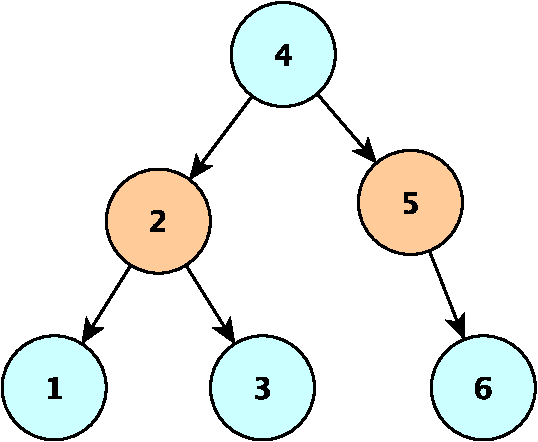
\includegraphics[width=0.5\textwidth]{illustrations/sets-crop.pdf}
\caption{Представление множества}
\label{fig:sets}
\end{figure}

На рисунке показаны красные и черные (ну ок, синие) узлы, на самом деле это может быть и AVL-дерево в зависимости от реализации. Главное -- что компаратор в некотором смысле задает структуру хранения данных.

Пользователь может указать любой компаратор, лишь бы он отвечал нескольким понятным условиям (так называемые отношения строгого порядка):

\begin {itemize}
\item Иррефлексивность: \lstinline!compare(x, x) == false!
\item Ассиметричность: \lstinline!x noteq y => compare(x, y) noteq compare(y, x)!
\item Транзитивность: \lstinline!compare(x, y) and compare(y, z) => compare(x, z)!
\end {itemize}

Множества поддерживают большинство стандартных операций над контейнерами рассмотренных в (\ref{StandardOperations}) причем некоторые поддержаны крайне оригинально.

\textbf{Вопрос к студентам:} как бы вы поддержали оператор ``меньше'' над множествами? Можете ли вы составить множество множеств с описанным вами оператором меньше? Является ли множество всех множеств в C++ собственным подмножеством?

\ifanswers
Много вариантов на самом деле. Простейший -- сравнивать размер, если размер второго аргумента больше размера первого возвращать true, иначе false.

Такой экзотики как множество всех множеств в C++ не бывает благодаря тому что каждый уровень инстанцирования шаблона задает по сути фон-Неймановский класс.
\fi

Кроме общих операций множества и мультимножества поддерживают специальные операции. Простые случаи такие как \lstinline!find! и \lstinline!count! понятны (\lstinline!find! возвращает \lstinline!set::end()! если ничего не найдено или итератор на элемент если он найден, \lstinline!count! же возвращает \lstinline!1! или \lstinline!0!, отвечая таким образом да или нет на вопрос о том есть ли элемент в множестве).

\begin{lstlisting}
template<class T> static inline bool 
contains(const std::set<T>& container, const T& value)
{
  return container.find(value) != container.end();
}
\end{lstlisting}

Более интересны \lstinline!lower_bound!, \lstinline!upper_bound! и \lstinline!equal_range!. Работают они так: \lstinline!lower_bound! возвращает итератор на первый элемент, который не меньше её аргумента, а \lstinline!upper_bound! -- на первый элемент, который больше её аргумента:

\begin{lstlisting}
std::set<int> s{4, 1, 3, 2, 5};
auto l = s.lower_bound(3);
auto u = s.upper_bound(3);
int prev = *--l;
int next = *++u;
\end{lstlisting}

\textbf{Вопрос к студентам:} чему равны next и prev?

\ifanswers
Верный ответ: конечно же 2 и 5 соответственно (2 потому что lower bound указывает на элемент 3, а 5 потому что upper bound указывает на 4).
\fi

Добавление элементов в мультимножество довольно просто: \lstinline!insert! добавляет элемент и возвращает итератор на добавленный элемент. Вопрос что делать с множеством если такой элемент уже есть? Два выхода -- либо возвращать пару \lstinline!pair <iterator, bool>! где итератор валиден только если второй элемент пары \lstinline!true!, либо возвращать хинт -- то есть на попытку добавить уже существующий элемент возвращать ссылку на этот элемент. Стандарт регламентирует обе возможности:

\begin{lstlisting}
std::pair<iterator,bool> insert( const value_type& value );
iterator insert( iterator hint, const value_type& value );
\end{lstlisting}

Особое значение hint реально было введено потому что функции нельзя перегружать по возвращаемому значению. Но потом было замечено, что если хорошо угадывать hint, так, чтобы была возможна вставка в позицию прямо перед ним, то амортизированное время вставки становится линейным. Это привело к добавлению специальной функции \lstinline!emplace_hint! для конструирования элемента максимально близко к указанному месту:

\textbf{Вопрос к студентам:}

\begin{lstlisting}
std::set<int> s{4, 1, 2, 5};
auto hint = /* something */ ;
s.insert(hint, 3);
\end{lstlisting}

Что здесь надо назначить hint, чтобы вставка прошла за O(1)?

\ifanswers
Верный ответ: \lstinline!s.upper_bound(3)!
\fi

Также в двух вариантах существует \lstinline!erase! -- она может брать на вход элемент и стирать все такие элементы или брать на вход позицию и удалять элемент, находящийся на этой позиции.

Важно: в принципе множества и мультимножества хранят изменяемые элементы. Но изменять их нельзя -- это выстрел себе в ногу.

\begin{lstlisting}
    std::set<int> s;
    s.insert(10);
    s.insert(20);

    iter = s.find(20);

    // OK?
    *iter = 0;
\end{lstlisting}

К счастью в новых версиях стандарта, итератор и константный итератор для множеств это теперь один тип.

\subsubsection{Карта и территория}

Часто вместе с ключом хочется хранить какое-нибудь значение -- например вместе со словом в словаре текста хранить количество раз, сколько оно встретилось в тексте. Вариант хранить его внутри множества -- не вариант, поскольку ключ, как показано выше не должен быть изменяемым.

Стандартная библиотека предлагает для этих целей специальные классы \lstinline!map! и \lstinline!multimap! отображающие множество ключей на множество значений.

\begin{lstlisting}
template < class Key, // map::key_type
           class T,   // map::mapped_type
           class Compare = less<Key>, 
           class Alloc = allocator<pair<const Key,T> >
           > class map;
\end{lstlisting}

Метод \lstinline!find! теперь выполянет более осмысленную работу:

\begin{lstlisting}
iterator find (const key_type& k);
\end{lstlisting}

возвращает итератор, который при разменовании даёт пару:

\begin{lstlisting}
typedef pair<const Key, T> value_type;
\end{lstlisting}

К результату поиска, вы можете обращаться с помощью стандартных для пар акцессоров \lstinline!first! и \lstinline!second!

\begin{lstlisting}
std::map<char,int> mymap;
std::map<char,int>::iterator it;
mymap.insert ( std::pair<char,int>('b',100) );
printf ("b is %d\n", mymap.find('b')->second);
\end{lstlisting}

Лучше заменить здесь явный конструктор на стандартную функцию \lstinline!make_pair!

Здесь что-то про вставку с квадратными скобками.

Тонкости возникают при удалении элементов:

\begin{lstlisting}
for (it = mymap.begin(); it != mymap.end(); ++it)
{
  if (it->second == 'b')
    mymap.erase (it); /* Boom! */
}
\end{lstlisting}

Поздравляю, вы только что спилили сук на котором сидите. Правильный способ:

\begin{lstlisting}
for (it = mymap.begin(); it != mymap.end(); ++it)
{
  if (it->second == 'b')
    mymap.erase (it++); /* Ok */
}
\end{lstlisting}

Ещё более правильный способ будет рассмотрен далее.

\subsubsection{Линейный обход ассоциативных контейнеров}

Ассоциативные контейнеры включают в себя множества (set) отображения (map), мультимножества (multiset) и мультиотображения (multimap).

Типичный пример работы с \lstinline!map! -- программа для подсчёта слов во входном файле и выдачи их частот в процентах.

\begin{lstlisting}
const int MAXLEN = 128;

int main(int argc, char** argv)
{
  char buf[MAXLEN];
  std::map <std::string, int> words;
  int count = 0;
  FILE *f;

  assert (argc > 0);

  f = fopen (argv[1], "r");
  assert (f != 0);

  while (std::fscanf(f, "%s", buf) > 0)
    {
      std::string word = buf;
      words[word] += 1;
      count += 1;
    }

  for (auto cur = words.begin();
       cur != words.end();
       cur++)
    fprintf (stdout, "%s -- %.3f%%\n", 
      cur->first.c_str(), 
      ((double)cur->second / count) * 100.0);

  return 0;
}
\end{lstlisting}

Надо понимать, что внутреннее представление \lstinline!map! это скорее всего красно-черное дерево. Интерфейс \lstinline!map <std::string, int>::iterator! позволяет устроить линейный inorder обход узлов дерева.

\subsubsection{Dependency graph}

TODO: здесь dep graph как хороший пример multimap

\pagebreak
\subsection{Потоки ввода/вывода}

Потоки ввода-вывода -- довольно спорная тема и именно поэтому они оставлены ``напоследок'' среди всех тем стандартной библиотеки. Их обзорное знание -- хороший тон, но стоит ли реально ими пользоваться -- большой вопрос (особенно учитывая, что стандарт C++11 предоставляет возможность соорудить безопасный относительно типов printf на variadic templates, см. \ref{TypesafePrintf}). В большинстве языков, спроектированных \textbf{позже} C++, ввод и вывод больше похожи на printf и scanf, чем на cin и cout. Например в предельно объектно ориентированном C\# это выглядит так

TODO: ну и как же

Это произошло от того, что в целом коммьюнити разочаровалось в потоках ввода-вывода и поэтому эти лекции не разделяют общего апологетического тона книг по C++ на эту тему. Но сначала -- общий обзор.

\subsubsection{Виды и иерархия потоков}

В программах на C привычными потоками (имеющими тип FILE*)

\subsubsection{Итераторы потоков ввода-вывода}

\begin{lstlisting}
const int N = 10;

/* function generator: */
int RandomNumber (void) { return (std::rand() % 20); }

/* less than class */
template <typename T>
class less_than_X
{
public:
  less_than_X(T x): m_x(x) {}

  bool operator() (const T &x) const
    {
      return (x < m_x);
    }
private:
  T m_x;
};

int main() 
{
  vector<int> v1(N), v2;
  less_than_X<int> pred(10); /* less than 10 instance */

  /* prefer generators to immediate fill */
  generate (v1.begin(), v1.end(), RandomNumber);

  /* some output to look at v1 */
  copy(v1.begin(), v1.end(), std::ostream_iterator<int>(cout, " "));
  cout << std::endl;

  remove_copy_if(v1.begin(), v1.end(), inserter(v2,v2.end()), pred);

  /* some output to be sure v2 contain more than 10 */
  copy(v2.begin(), v2.end(), std::ostream_iterator<int>(cout, " "));
  cout << std::endl;

  return 0;
}
\end{lstlisting}

\subsubsection{Форматированный ввод и вывод}

Для обеспечения форматированного ввода и вывода у потоков в стандартной библиотеке есть форматные модификаторы

\pagebreak
\subsection{Алгоритмы}

\hfill\textit{Computer science is no more about computers}

\hfill\textit{than astronomy is about telescopes}{\vspace{0.5em}}

\hfill\textit{-- Edsger W. Dijkstra}

TODO: тут классификация алгоритмов и их общий обзор

\subsubsection{Жизнь без явных циклов}

Алгоритмы позволяют ``в один вызов'' делать многие вещи, для которых в противном случае пришлось бы писать явные циклы. В разделе (\ref{vectorarrs}) рассматривался листинг невероятно полезной функции foo, которая выделяет вектор, инициализирует его и подсчитывает сумму его элементов. Подсчёт суммы элементов осуществлялся циклом. А как же иначе, спросите вы? Листинг ниже может показаться написанным очень непривычно:

\begin{lstlisting}
template <typename T>
T accum_op (T init, T elem)
{
  if (!check_legal(elem))
    throw std::runtime_error("Illegal element");
  return init + elem;
}

template <typename T>
T foo (int n)
{
  std::vector<T> t(n);
  init_t (&t[0], n);
  return std::accumulate (t.begin(), t.end(), 0, accum_op);
}
\end{lstlisting}

\textbf{Вопрос к студентам:} очевидно вместо \lstinline!accum_op! можно использовать лямбда-выражение. Перепишите этот код.

\ifanswers
Верный ответ: например
\begin{lstlisting}
return std::accumulate (t.begin(), t.end(), 0, 
           [](T init, T elem){return init + elem;});
\end{lstlisting}
\fi

Собственно, если приглядеться к функции \lstinline!foo()!, можно заметить в ней старую добрую функцию \lstinline!init()!, которая, скорее всего, внутри себя использует некий старый добрый цикл. Пусть она в ваших руках. Тогда переписав её на генератор \lstinline!init_elem!, который делает то же что и \lstinline!init()!, но для каждого элемента наособицу, можно переписать функцию \lstinline!foo()!, сделав явной генерацию элементов вектора. Поскольку её смысл становится совершенно явным, можно даже прекратить называть её \lstinline!foo()!, приведя крутизну её имени в соответствие с крутизной содержания. Итак встречайте обобщённый алгоритм \lstinline!generate_and_accumulate!.

\begin{lstlisting}
template <typename T, typename Acc, typename Gen>
T generate_and_accumulate (int n, T init_val, Acc accum_op, Gen init_op)
{
  std::vector<T> t(n);
  std::generate (t.begin(), t.end(), init_op);
  return std::accumulate (t.begin(), t.end(), init_val, accum_op);
}
\end{lstlisting}

Вот теперь это выглядит действительно круто.

Очевидно, что старая \lstinline!foo()! лишь её малозначащий частный случай:

\begin{lstlisting}
template <typename T> T init_op (void) { /* ... */ };
template <typename T> T accum_op (T init, T elem) { /* ... */ };

template <typename T> 
T foo (int n)
{
  return generate_and_accumulate (n, 0, accum_op, init_op);
}
\end{lstlisting}

Никаких явных циклов, никаких проблем с выделением и освобождением памяти и безопасностью исключений. Всё скрыто за средствами стандартной библиотеки и вы можете почувствовать себя программистом на Java. До первого подводного камня, конечно. Но чувство все равно сладко и приятно.

\subsubsection{Копирование диапазона}

\subsubsection{Пары итераторов для обозначения диапазона}

Обратите внимание что оба использованных выше алгоритма \lstinline!std::generate! и \lstinline!std::accumulate! для обозначения диапазона генерирования и аккумуляции, берут на вход пару итераторов. Это часто встречающаяся идиома и её истоки стоит рассмотреть подробней. Допустим, при написании класса \lstinline!vector!, появилась необходимость дать пользователю возможность сконструировать его из самых разных классов:

\begin{lstlisting}
template <class T>
class vector
{
  public:
    vector (const list<T> &); 
    vector (const set<T> &); 
    vector (const T * pod_array, int n); /* ! */
};
\end{lstlisting}

Следует обратить внимание, что в итоге получился разный интерфейс для конструирования из списка, который знает свою длину и из POD-массива, который свою длину не знает. Кроме того, конструкторов получилось слишком много. Пара итераторов здесь позволяет естественным образом обобщить идею ``диапазона'' в одном конструкторе:

\begin{lstlisting}
template <class T>
class vector
{
  public:
    /* Iterator-pair constructor */
    template <class InputIterator>
    vector (InputIterator begin, InputIterator end) 
};
\end{lstlisting}

Теперь любой список и множество могут сообщить вектору свои начало и конец, а POD-массив -- использовать для этого обычные указатели.

\subsubsection{Обобщенные циклы и range-based for}

Суть и сердце библиотеки C++ это абстрактные алгоритмы над обобщёнными контейнерами. Прекрасным примером такого кода является алгоритм \lstinline!for_each!, определённый примерно так:

\begin{lstlisting}
template <typename Iterator, typename Operation>
Operation for_each(Iterator act, Iterator end, Operation op)
{
  while(act != end)
    {
       op(*act);
       ++act;
    }
  return op;
}
\end{lstlisting}

Если третий параметр является обычной функцией, она будет вызвана для каждого разыменованного \lstinline!act!. 

\begin{lstlisting}
std::vector<int> v {0, 1, 2, 3, 4};
for_each (v.begin(), v.end(), 
          [](int x){cout << x;});
\end{lstlisting}

Использование такого алгоритма часто предполагает передачу туда пары итераторов \lstinline!begin! и \lstinline!end!, что является семантически обозначением ``Для всех элементов контейнера''. В новом стандарте можно записать это явно через range-based for\index{Range-based for}.

\begin{lstlisting}
for (auto n : v)
  cout << n;
\end{lstlisting}

Обычно используется аннотированный и уточненный вид  \lstinline!auto! чтобы не попадать на лишние копирования

\begin{lstlisting}
for (const auto &n : v)
  cout << n;
\end{lstlisting}

\subsubsection{Идиома erase-remove}

Удаление элементов из контейнера при работе с итераторами имеет свои контринтуитивные особенности. Формально для удаления служит алгоритм \lstinline!std::remove! и здесь может возникнуть искушение воспользоваться им что называется ``в лоб''.

\begin{lstlisting}
std::vector<int>& vec = myNumbers;
std::remove(vec.begin(), vec.end(), number_in);
\end{lstlisting}

Увы это не работает и не может работать. Ни у какого алгоритма не может быть достаточно информации чтобы по паре входных итераторов произвести честное удаление из обобщенного контейнера, потому что это потребовало бы от них по сути прямого управления памятью контейнера. Что происходит на самом деле проиллюстрировано ниже:

\begin{figure}[h!]
\centering
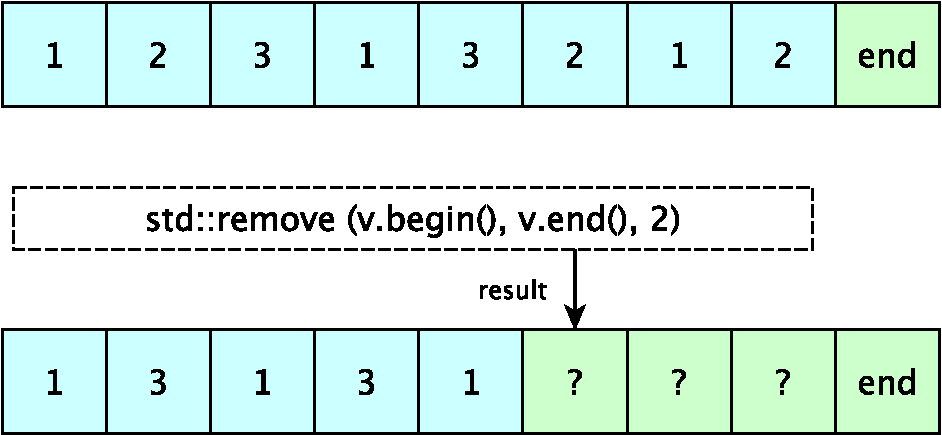
\includegraphics[width=0.9\textwidth]{illustrations/erase-remove-crop.pdf}
\caption{Идиома erase-remove}
\label{fig:erase_remove}
\end{figure}

Произошел сдвиг всех элементов, попадающих под условие удаления в хвост контейнера. Далее чтобы действительно очистить контейнер, нужно вызвать его метод \lstinline!erase! например так:

\begin{lstlisting}
std::vector<int>& vec = myNumbers;
vec.erase(std::remove(vec.begin(), vec.end(), number_in), vec.end());
\end{lstlisting}

Этот код записывается слитно очень часто, так что такие паттерны, как использование этой идиомы, опытный разработчик должен распознавать в коде ``на лету''.

\subsubsection{Трансформации и циклы}

\begin{lstlisting}
template <class MapT>
class eraseFct {
public:
  eraseFct(MapT* m) : theMap(m) {}
  void operator() (string nam)
  { typename MapT::iterator iter = theMap->find(nam);
    if (iter == theMap->end()) 
        throw invalid_argument(nam);
    theMap->erase(iter);
  }
private:
  MapT* theMap;
};

template <class MapT>
eraseFct<MapT> eraser(MapT* m) 
{ return eraseFct<MapT>(m); }
\end{lstlisting}

Подход с foreach

\begin{lstlisting}
map<string,info> directory_1;
// ... populate directory_1 ...
ifstream infile("toBeErased.txt");
for_each(istream_iterator<string>(infile),istream_iterator<string>(),
         eraser(&directory_1));
\end{lstlisting}

\subsubsection{Связывание функций-членов}

\begin{lstlisting}
std::transform(data_.begin(), data_.end(), data_.begin(), 
    std::bind(&CryptoModule::UndoCaesar, this, std::placeholders::_1)
);
\end{lstlisting}

\pagebreak
\subsection{Умные и слишком умные указатели}\label{SmartPointers}

\hfill\textit{I'm the one that has to die}

\hfill\textit{when it's time for me to die}{\vspace{0.5em}}

\hfill\textit{-- Jimi Hendrix}

Идиома RAII уже рассматривалась в (\ref{RAII}), и там же была сделана наивная попытка завернуть в класс для управления ресурсами такой классический разделяемый ресурс как дисковый файл. Конечно, идея обобщить RAII для любого \lstinline!T!, используя шаблоны -- приходит на ум почти сразу после знакомства с шаблонами. Паттерн обертки, осуществляющей управление временем жизни объекта умнее, чем это делается через обычный указатель, называется ``smart pointer'' или умный указатель. Таким образом это не какой-то класс, это общая концепция для целого семейства от крайне простых до крайне сложных и интересных классов.

\subsubsection{Первая попытка -- не слишком умный указатель}

Первая попытка написать не слишком сложную обертку для управления ресурсами, может выглядеть как-то так:

\begin{lstlisting}
template <typename T> 
class NotSoSmartP
{
private:
  T* pData; /* Generic pointer to be stored */
public:
  SP(T* pValue) : pData(pValue) {}
  ~SP() { delete pData; }
  T& operator* () { return *pData; }
  T* operator-> () { return pData; }
};
\end{lstlisting}

Самое главное здесь это перегрузка двух интересных операторов -- \lstinline!operator*! который называется \textbf{dereferencing} т.е. разыменование и \lstinline!operator->! который называется \textbf{indirection} т.е. косвенный доступ. Но далее они часто будут называться просто ``звёздочка'' и ``стрелочка''.

Пусть есть класс \lstinline!Polynom! определенный как-то так:

\begin{lstlisting}
class Polynom
{
public:
  Polynom (int size, ...);
  Polynom (const Polynom & rhs);
  ~Polynom ();
  void display ();
  /* ... */
}
\end{lstlisting}

Его можно использовать вместе с умным указателем как-то так:

\begin{lstlisting}
  NotSoSmartP<Polynom> p(new Polynom(5, 1, 2, 3, 4, 5));
  p->display();
  /* no need to delete */
\end{lstlisting}

Особое внимание следует обратить, что метод умного указателя вызывается так, как если бы действительно вызывался метод класса \lstinline!Polynom! по указателю на него.

Но первая проблема обнаруживается сразу же:

\begin{lstlisting}
  NotSoSmartP<Polynom> p(new Polynom(5, 1, 2, 3, 4, 5));
  NotSoSmartP<Polynom> q = p;
  p->display();
  /* boom! */
\end{lstlisting}

И действительно -- обычное копирование или создание по образцу такого указателя приведет к ошибке двойного удаления (см. \ref{RAII}). Что тут можно сделать? Самый простой способ -- запретить копирование и присваивание. Эта стратегия называется ``scoped pointer'' и именно так устроен и работает класс \lstinline!boost::scoped_ptr!. Но это все ещё не самая умная стратегия. Очевидно есть две более разумные вещи -- обеспечить уникальность владения объектом и передачу владения при некоторых обстоятельствах или обеспечить безопасное совместное владение объектом и -- в той или иной форме -- подсчет ссылок.

\subsubsection{Стандартные умные указатели}

TODO: продолжить раздел

\subsubsection{Проблема COAP и небольшая экскурсия в новый стандарт}\label{COAP}

TODO: продолжить раздел

\subsubsection{Ещё более умные указатели}

TODO: продолжить раздел

\subsection{Память своими руками}

Интересной идеей в стандартной библиотеке C++ является идея аллокатора. Аллокатором называется класс, инкапсулирующий в себе стратегию выделения и освобождения памяти. Большинство стандартных контейнеров используют аллокаторы. Скажем полное определение уже упоминавшегося в (\ref{vectorarrs}) класса \lstinline!vector! на самом деле выглядит вот так:

\begin{lstlisting}
template <class T, class Allocator = allocator<T> > class vector;
\end{lstlisting}

Поэтому каждый раз, когда создается вектор, у него на самом деле пропускается один параметр:

\begin{lstlisting}
std::vector <int> myvec; /* brief form */
std::vector <int, allocator<int> > myvec; /* full form */
\end{lstlisting}

В связи с этим полезно знать что такое аллокаторы и как они работают.

\subsubsection{Пользовательские аллокаторы}

Аллокатор это шаблон для того типа, для которого он аллоцирует:

\begin{lstlisting}
template<typename T>
class Allocator {
\end{lstlisting}

В открытой части аллокатор должен определять несколько стандартных имён, например так:

\begin{lstlisting}
    typedef T value_type;
    typedef value_type* pointer;
    typedef const value_type* const_pointer;
    typedef value_type& reference;
    typedef const value_type& const_reference;
    typedef std::size_t size_type;
    typedef std::ptrdiff_t difference_type;
\end{lstlisting}

Шаблонная вложенная структура \lstinline!rebind! обрабатывает случаи, когда на самом деле созданию подлежат иные типы, чем \lstinline!T!. Скажем \lstinline!list<int>! создаёт не целые числа, а узлы списка. Это внутреннее превращение и называется rebinding:

\begin{lstlisting}
    template<typename U>
    struct rebind {
        typedef Allocator<U> other;
    };
\end{lstlisting}

Стандартная функция \lstinline!address! должна возвращать \lstinline!pointer! или \lstinline!const_pointer!.

\begin{lstlisting}
    inline pointer address(reference r) { return &r; }
    inline const_pointer address(const_reference r) { return &r; }
\end{lstlisting}

Сердце аллокатора: функции выделения и освобождения памяти. Именно здесь можно развернуться с гениальными стратегиями.

\begin{lstlisting}
    inline pointer allocate(size_type cnt, 
       typename std::allocator<void>::const_pointer = 0) { 
      return reinterpret_cast<pointer>(::operator new(cnt * sizeof (T))); 
    }
    inline void deallocate(pointer p, size_type) { 
        ::operator delete(p); 
    }
\end{lstlisting}

Бывает полезно ограничить размер доступной памяти (если, например, речь о выделении из статического буфера).

\begin{lstlisting}
    inline size_type max_size() const { 
        return std::numeric_limits<size_type>::max() / sizeof(T);
    }
\end{lstlisting}

Считается, что пользовательские \lstinline!construct! и \lstinline!destroy! могут очень сильно отличаться от стандартного размещающего \lstinline!new!.

\begin{lstlisting}
    inline void construct(pointer p, const T& t) { new(p) T(t); }
    inline void destroy(pointer p) { p->~T(); }
\end{lstlisting}

Как ни странно, аллокаторы чтобы быть совместимыми требуют сравнения на рвенство и неравенство.

\begin{lstlisting}
    inline bool operator==(Allocator const&) { return true; }
    inline bool operator!=(Allocator const& a) { return !operator==(a); }
\end{lstlisting}

Кода вы разрабатываете свой аллокатор, вы должны быть уверены, что знаете что вы делаете и зачем вам это нужно. В библиотеке Intel Threading Building Blocks например реализовал собственный аллокатор и утверждается, что производительность вектора в многопоточном приложении можно существенно улучшить, объявив его как:

\begin{lstlisting}
std::vector<T,tbb::scalable_allocator<T> >
\end{lstlisting}

Ещё примеры -- аллокаторы рассчитанные на ограниченное количество памяти в EASTL, собственные аллокаторы из файла. Скорее всего вам никогда не придется все это писать.

\pagebreak
\subsection{Домашняя наработка по стандартной библиотеке}

\pagebreak
\section{Новые горизонты}

TODO: этот раздел был недавно расформирован в пользу других разделов куда были перенесены уже не новые возможности: вывод типов, правые ссылки, прочее. Тут нужно новое вступление, что-нибудь про C++17 и все такое.

Примерный план:

concepts (сюда же contracts)

modules (если войдут в 17-й)

co-routines

SIMD

filesystem

asio

Плюс от C++14 здесь остается многопоточность потому что неясно куда её (возможно asio будет её расширением).

\pagebreak
\subsection{Концепты\index{Concepts}}\label{Concepts}

\hfill\textit{Thoughts without content are empty,}

\hfill\textit{intuitions without concepts are blind}{\vspace{0.5em}}

\hfill\textit{-- Immanuel Kant}

Любую компьютерную программу читает (и иногда пишет) разработчик, который оперирует семантическим смыслом выражений языка программирования. При этом у разработчика есть очень большое количество корректных синтаксических форм для семантически эквивалентных конструкций.

Но ту же программу читает (обрабатывает) компилятор, который не понимает её смысла. Вместо этого компилятор механически упрощает выражения и трансформирует их, ориентируясь на их финальное представление в целевой архитектуре. Так выражению имеющему смысл сложения величин могут быть сопоставлены принципиально разные инструкции ассемблера в зависимости от того являются эти числа целыми или с плавающей точкой.

Именно тот факт, что смысл выражений высокоуровневых языков часто совершенно не зависит от типов и конкретной интерпретации этих выражений, позволяет обобщенное программирование как таковое.

Почти классический пример обобщенного кода: функция для нахождения элемента в диапазоне (диапазон здесь может быть вектором, списком, декой, множеством, пользовательским типом, согласующимся с сокращенным синтаксисом \lstinline!for!). Это (а также тип элемента) серьёзно повлияет на конкретный сгенерированный код, но совсем не повлияет на смысл следующей простой конструкции:

\begin{lstlisting}
template<typename R, typename T> bool 
in (R const& range, T const& value) 
{
  for (auto const& x : range)
    if (x == value)
      return true;
  return false;
}
\end{lstlisting}

\textbf{Вопрос к студентам}: что будет при попытке использовать этот код неправильно, например ``найти'' число в векторе строк?

\begin{lstlisting}
vector<string> v { "0", "1", "2" };
bool is_in = in (v, 0);
\end{lstlisting}

%\ifanswers
Очевидно ошибка компиляции. Главная проблема в том, что это будет \textbf{неприятная} ошибка компиляции:

\begin{verbatim}
In file included from /home/tilir/Applications/gcc-5.2/include
/c++/5.2.0/bits/stl_algobase.h:67:0,
                 from /home/tilir/Applications/gcc-5.2/include
/c++/5.2.0/vector:60,
                 from constr1.cc:1:
/home/tilir/Applications/gcc-5.2/include/c++/5.2.0/bits
/stl_iterator.h:820:5: note: candidate: 
template<class _IteratorL, class _IteratorR, class _Container> 
bool __gnu_cxx::operator==(const __gnu_cxx::__normal_iterator
<_IteratorL, _Container>&, const __gnu_cxx::__normal_iterator
<_IteratorR, _Container>&)
     operator==(const __normal_iterator
<_IteratorL, _Container>& __lhs,
     ^
/home/tilir/Applications/gcc-5.2/include/c++/5.2.0/bits
/stl_iterator.h:820:5: note:   template argument deduction
/substitution failed:
constr1.cc:10:11: note: ‘const std::__cxx11::basic_string<char>’ 
is not derived from ‘const __gnu_cxx::__normal_iterator
<_IteratorL, _Container>’
     if (x == value)
\end{verbatim}

Это только крошечный кусочек из простыни которую выдаст gcc-5.2
%\fi

\textbf{Домашняя наработка:} попробуйте скомпилировать ещё более простой код:

\begin{lstlisting}
class X {};
std::set<X> x;
x.insert(X{});
\end{lstlisting}

В своё время обобщенное программирование на C++ сильно споткнулось об это. Эти знаменитые простыни ошибок, которые заставляли даже опытных разработчиков кричать и плакать как детей, увы, неизбежны. Шаблоны добавляют лишний шаг к компиляции программы: сначала должны быть инстанциированы типы, потом скомпилирован код. В случае если инстанцирование создало большой стек, будет много ошибок, без рациональной возможности сократить их, если нет механизмов ограничить шаблонный полиморфизм и заблокировать собственно инстанцирование. Между прочим, безо всякого шаблонного инстанцирования точно таких же безумных ошибок можно добиться макросами.

\begin{lstlisting}
#include __FILE__
p;
\end{lstlisting}

Идея здесь та же -- макроподстановка никак не ограничена. Но макроподстановка не Тьюринг полна, поэтому в макросах это менее актуально (там обычно просто нет достаточно большого стека подстановки чтобы развернуться). Хотя если кто-то хоть раз пробовал boost preprocessor, он знает боль. А в шаблонах рекурсивные вызовы -- обычное дело. И тем важнее добиться того, чтоб неправильные ветки отсекались как можно раньше.

Итак ключ к обоснованию нововведений в языке и главная тема этой лекции: \textbf{ограничение шаблонного полиморфизма}.

Ограничить шаблонный полиморфизм -- также хорошая идея для разделения типов: иногда хотелось бы такой обобщенный тип, который ведет себя по разному когда инстанцирован чем-то вроде целого или чем-то вроде плавающего числа (может быть даже имеет разные методы).

Итак, ограничений и контроля полиморфизма в языке явно не хватало. И, конечно, все всегда понимали, что с этим надо что-то делать. За много лет коммьюнити наработало некий опыт.

\subsubsection{Добрые старые способы контроля полиморфизма}

В этом разделе будут рассмотрены методы, работающие для C++14. Поскольку это часто связано с написанием большого количества кода, лучше в качестве рабочего примера рассмотреть очень простую обобщенную функцию проверки значений двух разных типов на равенство.

\begin{lstlisting}
template <typename T, typename U> bool
check_eq (T &&lhs, U &&rhs) {
  return (lhs == rhs);
}
\end{lstlisting}

Её также можно использовать правильно или ошибочно.

\begin{lstlisting}
// no operator ==  here
struct noeq {
  noeq (int x) {}
};

int main (void) {
  check_eq (1, 1);       // ok
  check_eq (1, 1.0);     // ok
  check_eq (1, noeq(1)); // problems
  return 0;
}
\end{lstlisting}

В случае ошибочного использования, ошибка компиляции выглядит очень простой:

\begin{verbatim}
eqcomp00.cc: In instantiation of 
  ‘bool check(T&&, U&&) [with T = int; U = noeq]’:
eqcomp00.cc:13:20:   required from here
eqcomp00.cc:3:15: error: no match for 
  ‘operator==’ (operand types are ‘int’ and ‘noeq’)
   return (lhs == rhs);
\end{verbatim}

Но, тем не менее, хотелось бы вместо неё иметь нечто осмысленное.

Простейший способ, и, обычно, первый, который приходит в голову новичку, это влепить статическую проверку.

\begin{lstlisting}
static_assert (is_equality_comparable<T, U>::value, 
              "Comparable types required");
\end{lstlisting}

Для этого надо сначала понять, что такое \lstinline!is_equality_comparable!. В стандарте C++14 ничего такого нет, но хороший программист без труда спляшет это ограничение на SFINAE в C++14.

\begin{lstlisting}
template <typename T, typename U, typename = void>
struct is_equality_comparable : std::false_type {};

// I feel really C++ here
template <typename T, typename U>
struct is_equality_comparable <T, U,
    decltype ((void)(std::declval<T&>() == std::declval<U&>()))
  > : std::true_type {};
\end{lstlisting}

Стало ли лучше?

\begin{verbatim}
eqcomp00.cc: In instantiation of 
  ‘bool check(T&&, U&&) [with T = int; U = noeq]’:
eqcomp00.cc:28:27:   required from here
eqcomp00.cc:16:3: error: static assertion failed: 
   Comparable types required
   static_assert (is_equality_comparable<T, U>::value, 
   ^
eqcomp00.cc:18:15: error: no match for 
   ‘operator==’ (operand types are ‘int’ and ‘noeq’)
   return (lhs == rhs);
\end{verbatim}

Стало хуже. Мы получили static assertion failure и, \textbf{вдобавок} к нему, также instantiation failure.

Проблема в том, что эти ошибки проявляются \textbf{поздно}. Компилятор уже начал инстанцирование шаблона и он уже прошел по этому пути достаточно далеко. Наличие или отсутствие failures далее ничего не значат. Таким образом, \lstinline!static_assert! в языке нужен не для этого. Он не мешает компилятору разобрать функцию, а защищает от ошибок, которые вызваны несовпадением статических контрактов.

Гораздо интереснее использовать \lstinline!enable_if!, который даёт возможность выбросить функцию из рассмотрения:

\begin{lstlisting}
// Wow, I am even MORE C++ now
template <typename T, typename U,
          typename = std::enable_if_t <
             is_equality_comparable<T, U>::value>
          >
bool check (T &&lhs, U &&rhs);
\end{lstlisting}

В \lstinline!enable_if<false, T>! нет зависимого типа \lstinline!enable_if<false, T>::type! и происходит классический случай SFINAE, см. (\ref{SFINAE}).

Ошибка выглядит более вразумительно:

\begin{verbatim}
eqcomp01.cc:27:20: error: 
  no matching function for call to ‘check(int, noeq)’
   check (1, noeq(1));

eqcomp01.cc:18:6: note: candidate: 
  template<class T, class U, class> bool check(T&&, U&&)
  bool check (T &&lhs, U &&rhs);
       ^
eqcomp01.cc:18:6: note:   
  template argument deduction/substitution failed
\end{verbatim}

Инстанцирования такой функции просто не происходит. Тем не менее, сложно не заметить, что синтаксис для вышивания на \lstinline!enable_if! переусложнен и требует для блокирования подстановки завязываться на третий шаблонный параметр, который в общем не при чём.

\subsubsection{Простые ограничения\index{Constraints}}\label{Constraints}

Введение в новый стандарт синтаксического сахара для таких конструкций было практически неизбежным.

\begin{lstlisting}
template <typename T, typename U>
requires is_equality_comparable<T, U>::value
bool check (T &&lhs, U &&rhs);
\end{lstlisting}

Теперь правильное использование всё так же идёт без ошибок. В то же время неправильное использование выдает простую ошибку:

\begin{verbatim}
eqcomp01s.cc: In function ‘int main()’:
eqcomp01s.cc:27:20: error: cannot call function 
  ‘bool check(T&&, U&&) [with T = int; U = noeq]’
   check (1, noeq(1));
                    ^
eqcomp01s.cc:18:6: note:   constraints not satisfied
 bool check (T &&lhs, U &&rhs);
      ^~~~~
eqcomp01s.cc:18:6: note:   
   ‘is_equality_comparable<T, U>::value’ evaluated to false
\end{verbatim}

Главное в этой ошибке то, что она, как и в случае \lstinline!enable_if!, выдается \textbf{рано}, то есть задолго до того, как компилятор реально полез инстанцировать что бы то ни было. Sutton сообщал об уменьшении времени компиляции хорошо ограниченного таким образом кода на десятки процентов.

Явная запись \lstinline!requires! в таком контексте называется ограничением (constraint) и в данном случае использует для проверки ограничения функцию стандартной библиотеки.

Также это является \textit{requires-clause} -- собственно ограничением. Немного позже будут введены \textit{requires-expressions} -- то, что будет называться ограничивающими выражениями. Уже сейчас хочется предупредить, что их нельзя путать.

Несмотря на то, что в этом разделе ограничения вводятся как ограничения для обобщенного программирования, на самом деле в них нет ничего магического: это обычный C++ и они могут использоваться с обычными функциями.

\begin{lstlisting}
void f ()
requires sizeof(int) == 4
{
 /* do something */
}
\end{lstlisting}

И даже более того, нешаблонные функции могут быть ограничены охватывающими шаблонными параметрами.

\begin{lstlisting}
template <typename T>
class vector {
  // ....
  // we have copy ctor only if T copyable
  requires std::is_copyable<T>::value
  vector (const vector&);
};
\end{lstlisting}

\textbf{Домашняя наработка:} попробуйте такое сделать на \lstinline!enable_if! просто чтобы понять масштаб упрощения.

Констрейнты работают лениво: возможное нарушение размера целого будет проверено только в точке вызова этой функции. Нет вызова -- нет проблем.

\textbf{Вопрос к студентам:} кстати об ограничениях на ограничения. А как вы думаете, виртуальные функции могут быть ограничены подобным образом?

\ifanswers
Правильный ответ: конечно не могут (примерно по тем же причинам, по каким они не могут быть шаблонными). В таблице виртуальных функций просто нет места для этого признака, а связывать его со статическим типом чревато проблемами.
\fi

\subsubsection{Пример -- перегрузка конструкторов}

Во многих случаях даже простых констрейнтов достаточно, чтобы чудесно упрощать код. Типичная задача -- внутри обобщенного класса иметь отдельно конструктор из плавающих и отдельно из целочисленных типов (пример взят из доклада Роджера Орра на ACCU 2016). 

Если решать эту задачу на бумажке, на ум приходит решение в старом добром стиле.

\begin{lstlisting}
struct Foo {
  enum {int_like, float_like} type_;

  template <typename Int, 
            typename = std::enable_if_t<
              std::is_integral<Int>::value>
            >
  Foo (Int x) : type_(int_like) { 
    std::cout << "int like: " << x; 
  }

  template <typename Float, 
            typename = std::enable_if_t<
              std::is_floating_point<Float>::value>
            >
  Foo (Float x) : type_(float_like)  { 
    std::cout << "float like: " << x; 
  }
};

int main () {
  Foo (1);
  Foo (5.0);
  return 1;
}
\end{lstlisting}

Увы, у него есть небольшой недостаток -- оно не скомпилируется.

\begin{verbatim}
ctorex01.cc:13:3: error: 
  ‘template<class Float, class> Foo::Foo(Float)’ 
   Foo (Float x) : type_(float_like)     
   ^~~
ctorex01.cc:9:3: error: with 
  ‘template<class Int, class> Foo::Foo(Int)’
   Foo (Int x) : type_(int_like)
\end{verbatim}

Шаблонные функции просто не могут быть перегружены по имени шаблонного параметра. Впрочем, танки грязи не боятся и немного времени в отладчике приводит к более интересному решению.

\begin{lstlisting}
struct Foo {

  enum {int_like, float_like} type_;

  template <int> struct dummy { dummy(int) {} };

  template <typename Int,
            typename = std::enable_if_t<
              std::is_integral<Int>::value>
            >
  Foo (Int x, dummy<0> = 0) : type_(int_like)
  {
    std::cout << "int like: " << x << std::endl;
  }

  template <typename Float,
            typename = std::enable_if_t<
              std::is_floating_point<Float>::value>
            >
  Foo (Float x, dummy<1> = 0) : type_(float_like)
  {
    std::cout << "float like: " << x << std::endl;
  }
};
\end{lstlisting}

Теперь все хорошо, но опять ценой некоторой избыточности. В то же время даже с самыми простыми ограничениями та же задача решается как персик.

\begin{lstlisting}
struct Foo {

  enum {int_like, float_like} type_;

  template <typename Int>
  requires std::is_integral<Int>::value
  Foo (Int x) : type_(int_like)
  {
    std::cout << "int like: " << x << std::endl;
  }

  template <typename Float>
  requires std::is_floating_point<Float>::value
  Foo (Float x) : type_(float_like)
  {
    std::cout << "float like: " << x << std::endl;
  }

};
\end{lstlisting}

Со скромной точки зрения автора, даже если бы ограничения ввели только в виде простых ограничений, это серьёзно разгрузило бы метапрограммирование во многих практически важных контекстах.

\subsubsection{Сложные ограничения}

Простыми ограничениями можно написать три вида выражений: предикаты, конъюнкции предикатов и дизъюнкции предикатов.

\textbf{Вопрос к студентам:} пусть задан предикат:

\begin{lstlisting}
template <typename T>
constexpr int somepred() {
  return 14;
}
\end{lstlisting}

выполняются или нет указанные констрейнты для функции \lstinline!check! если первый терм ложен?

\begin{lstlisting}
template <typename T, typename U>
requires is_equality_comparable<T, U>::value &&
         (somepred<T>() == 14) || 
         (somepred<U>() == 42)
bool check (T &&lhs, U &&rhs);
\end{lstlisting}

\ifanswers
Правильный ответ: конечно нет, так как \lstinline!false && true || false! по обычной схеме дает false
\fi

К сожалению, это не всё, что может быть нужно от ограничений. Простой пример: как избавиться от всё ещё необходимого шаблонного определения \lstinline!is_equality_comparable!? Для этого может быть использовано сложное ограничение, использующее ограничивающие выражения (requires-expressions).

\begin{lstlisting}
template <typename T, typename U>
requires requires(T t, U u) { t == u; }
bool check (T&& lhs, U&& rhs);
\end{lstlisting}

Ключевое слово \lstinline!requires! упомянутое дважды делает именно это -- открывает ограничение, после чего вместо предиката использует в нем ограничивающее выражение.

Ограничивающие выражения похожи на константно-выраженные (constexpr) функции. Но в них есть своя магия. Она заключается в том, что сложные ограничения никогда не вычисляются, в этом они похожи на выражения-параметры decltype. Для них только проверяются типы. Это создаёт громадную разницу между двумя формами ограничений

\begin{lstlisting}
// (1) constexpr function somepred ct evaluated
template <typename T>
requires somepred<T>() == 42
bool foo (T&& lhs, U&& rhs);

// (2) constexpr function somepred typechecked only
template <typename T>
requires requires (T t) { 
  somepred<T>() == 42;
}
bool bar (T&& lhs, U&& rhs);
\end{lstlisting}

Именно это делает сложные ограничения сложными.

Есть три основных категории сложных ограничивающих выражений:

\begin{enumerate}
\item Базовые ограничивающие выражения -- проверяют наличие операции над типами и на этом всё.

\begin{lstlisting}
template <typename T>
requires requires (T a, T b) {
           a + b;
         }
T test1 (T, T);
\end{lstlisting}

Есть некое тонкое различие между simple и expression requirements, выше указана первая форма, но это уже очень тонкая разница.

\item Ограничивающие выражения для типов -- проверяют наличие типа.

\begin{lstlisting}
template <typename T>
requires requires() {
           typename T::inner;
         }
T test2 (T, T);
\end{lstlisting}

\item Составные ограничивающие выражения -- проверяют и операцию и выводимый тип.

\begin{lstlisting}
template <typename T>
requires requires(T x) {
           {*x} -> typename T::inner;
         }
T test3 (T, T);
\end{lstlisting}

\end{enumerate}

Кроме этих ограничений есть ещё ограничения на спецификацию исключений и прочая экзотика, которую можно прочитать в очередном TS, но чтобы составить общее впечатление достаточно различать эти три вида.

Немножко практики. Пусть даны структуры, отвечающие некоторым из упомянутых выше требований.

\begin{lstlisting}
struct HasInner {
  using inner = int;
};

struct HasDeref {
  using inner = int;
  inner operator*();
};
\end{lstlisting}

Можно посмотреть какие выполняются и не выполняются в каких случаях.

\begin{lstlisting}
int
main (void) {
  test1(1, 1);
  test1(HasInner{}, HasInner{}); // no +
  test2(HasInner{}, HasInner{});
  test2(1, 1); // no inner
  test3(HasDeref{}, HasDeref{});
  test3(HasInner{}, HasInner{}); // no deref
}
\end{lstlisting}

Разумеется сложные ограничивающие выражения можно комбинировать.

\begin{lstlisting}
template <typename T>
requires requires(T x) {
           {*x} -> typename T::inner;
         } &&
         requires() {
           typename T::inner;
         } &&
         requires (T a, T b) {
           a + b;
         }
T test4 (T, T);
\end{lstlisting}

\textbf{Вопрос к студентам:} написать тип, который подойдет под такое ограничение.

\ifanswers
Вариант ответа:
\begin{lstlisting}
struct HasPlus {
  using inner = int;
  inner operator*();
  void operator+(HasPlus x);
};
\end{lstlisting}
\fi

Сложные ограничения позволяют очень многое (неожиданно многое) но они имеют несколько сложный синтаксис, поэтому сложные примеры следует отложить до введения простого способа выносить сложные ограничения в общую часть -- собственно концептов (мы до них добрались, да).

\subsubsection{Простые концепты}

Выше уже можно было увидеть, что сложные ограничения могут быть очень сложны, а главное -- всегда есть желание их переиспользовать, а не писать каждый раз заново.

Например можно прикинуть какой интерфейс должен поддерживать тип, чтобы быть последовательностью с обратной вставкой (Sequence)? На ум приходит следующее.

\begin{enumerate}
\item тип \lstinline!T::element_type! для указания своего типа элементов
\item метод \lstinline!size()! для проверки размера, возвращающая \lstinline!size_t!
\item метод \lstinline!empty()! для проверки пустоты, возвращающий \lstinline!bool!
\item метод \lstinline!back()! для получения последнего элемента, возвращающий \lstinline!T::element_type!
\item метод \lstinline!push_back()! для вставки в конец последовательности
\end{enumerate}

Простой концепт для такого класса типов можно определить как (это можно пошагово разобрать у доски).

\begin{lstlisting}
template <typename T>
concept bool Sequence() {
  return
    requires { typename T::element_type; } &&
    requires (T t, typename T::element_type x) {
      { t.size() } -> size_t;
      { t.empty() } -> bool;
      { t.back() } -> typename T::element_type;
      { t.push_back(x) } // not specified (!)
    };
}
\end{lstlisting}

Есть несколько форм эквивалентного синтаксиса, в которых можно использовать получившийся концепт:

\begin{enumerate}

\item Базовый синтаксис -- явное использование в ограничении 
\begin{lstlisting}
template <typename T> 
requires Sequence<T>
void fill_with_random (T &x, int n);
\end{lstlisting}

\item Упрощенный синтаксис -- вынос констрейнта в шаблонный параметр

\begin{lstlisting}
template <Sequence T> 
void fill_with_random (T &x, int n);
\end{lstlisting}

\item Синтаксис с выводом типов:

\begin{lstlisting}
void fill_with_random (Sequence &x, int n);
\end{lstlisting}

\end{enumerate}

Последний вариант выглядит несколько странно (и вызывает обоснованную критику), но в языке уже включена в стандарт C++17 возможность эквивалентно писать формы для обычных функций с шаблоном и с \lstinline!auto!.

\begin{enumerate}
\item Форма обычного шаблона функции 
\begin{lstlisting}
template <typename T> 
void foo (T x);

template<typename T, typename U, typename V> 
void bar(T (U::*)(V));
\end{lstlisting}
\item Форма с выводом типов
\begin{lstlisting}
void foo (auto x);

void bar(auto (auto::*)(auto));
\end{lstlisting}

\end{enumerate}

В свете этого идея такого же вывода концептами находится вполне в русле преобразований в язык. Аналогично в языке уже (с 14-го года) существуют обобщенные лямбды. Аналогично нет ничего противоестественного в том, чтобы ограничивать их концептами.

\begin{enumerate}
\item Обобщенная лямбда
\begin{lstlisting}
find_if(v, [str](const auto& x) 
           { return str == x; });
\end{lstlisting}
\item Ограниченная обобщенная лямбда
\begin{lstlisting}
find_if(v, [str](const String& x)
           { return str == x; });
\end{lstlisting}
\end{enumerate}

Есть некие ограничения на то, как могут быть устроены простые концепты-функции: они всегда возвращают \lstinline!bool!, никогда не принимают аргументов, состоят только из одного \lstinline!return! (похоже на старые добрые константно-выраженные функции в C++11) и не могут быть ни объявлены а позже определены, ни сделаны функциями-членами, ни быть друзьями классов. И конечно, в отличии от аргументов \lstinline!constexpr! функций, аргументы концептов не могут быть ограничены в свою очередь концептами.

Концепты (в рамках COncepts Lite) не проверяют семантику, то есть нельзя проверить, что

\begin{lstlisting}
t.empty() == (t.size() == 0)
\end{lstlisting}

Концепты также не проверяют реализацию: пользователь может заложиться внутри шаблона на неявный интерфейс не предусмотренный концептом

\begin{lstlisting}
template<Range R, typename T> bool
requires RangeEqComparable<R, T>()
in (R const& range, T const& value) {
  for (auto const& x : range)
    if (x != value) // OOPS!
      return false;
  return true;
}
\end{lstlisting}

Этот пункт вызывает споры и критику. Многие считают, что как раз проверять реализацию шаблона -- важное предназначение концептов как инструмента.

В рассмотренном выше примере, концепт \lstinline!Sequence! состоял только из сложных ограничений, но можно делать концепты и из простых ограничений.

\begin{lstlisting}
template <typename C> 
concept bool isInt() { 
  return std::is_integral<C>::value;
}
\end{lstlisting}

Мало того, концепты вообще не обязаны быть функциями. Самые простые концепты получаются из шаблонных переменных.

\begin{lstlisting}
template <typename C> 
concept bool Int = std::is_integral<C>::value;
\end{lstlisting}

Это работает так же как обычные шаблонные переменные. Можно записать даже проще.

\begin{lstlisting}
template <typename T>
concept bool Int = is_integral_v<T>;

template <typename T>
concept bool Float = is_floating_point_v<T>;
\end{lstlisting}

Здесь использован явный синтаксис присваивания концепту шаблонна переменной (по сути присваивание на метаклассах).

Увы, концепты не поддерживают рекурсию и поэтому не Тьюринг-полны. Также их нельзя специализировать. Зато возможна частичная специализация по констрейнту:

\begin{lstlisting}
template <typename T>
class complex;

template <Float T>
class complex { /* complex numbers */ };

template <Int T>
class complex { /* gaussian integers */ };
\end{lstlisting}

Это похоже на пример с конструкторами, но выглядит ещё более симпатично. Самое интересное: любой (даже тривиальный как C1 выше) констрейнт ограничивая шаблон делает его более специализированным, чем не ограниченный шаблон.

Не менее красиво выглядит теперь и пример с перегрузкой конструкторов:

\begin{lstlisting}
struct Foo {
  enum {int_like, float_like} type_;
  Foo (Int x);
  Foo (Float x);
};
\end{lstlisting}

Тем не менее, иногда нетривиальный концепт может быть довольно сложен. Поэтому простые концепты можно писать в терминах ещё более простых. Например для уже рассматривавшейся проверки на сравнимость на равенство можно соорудить вот такое:

\begin{lstlisting}
template <typename T, typename U>
concept bool Weak_equality_comparable() {
  return requires(T t, U u) {
    {t == u} -> bool;
  };
}

template <typename T, typename U = T>
concept bool Equality_comparable() {
  return Weak_equality_comparable<T, U>() &&
         Weak_equality_comparable<U, T>();
}
\end{lstlisting}

Но вот в том как воспользоваться таким концептом для определения функции \lstinline!check()! есть тонкости.

\textbf{Вопрос к студентам:} сработает ли вот такой вариант?

\begin{lstlisting}
template <Equality_comparable T,
          Equality_comparable U>
bool check(T, U);
\end{lstlisting}

\ifanswers
Он сработает, но не так как можно ожидать: будет проверено что \lstinline!T! сравнимо с \lstinline!T! и что \lstinline!U! сравнимо с \lstinline!U!. Но программист скорее всего хочет проверить, что \lstinline!T! сравнимо с \lstinline!U!.
\fi

Для решения этой задачи можно использовать либо явный синтаксис с ограничением, либо принципиально новый синтаксический выверт -- введение шаблона.

\begin{lstlisting}
Equality_comparable{T, U}
bool check(T, U);
\end{lstlisting}

Эта запись является сокращением для

\begin{lstlisting}
template <typename T, typename U>
requires Equality_comparable<T, U>()
bool check(T, U);
\end{lstlisting}

И выглядит довольно интересно. Также столь удобный синтаксис позвоялет заменить \lstinline!auto! на концепт:

\begin{lstlisting}
template <typename C> 
concept bool Int = std::is_integral<C>::value;

// ...

Int x = f(x); // auto x = f(x);
\end{lstlisting}

Благодаря концепту теперь в коде будет яснее чего ожидать от вывода типов (ну и усилится проверка от человеческих ошибок).

\subsubsection{Вариабельные концепты}

Ещё один пример полезного использования получившегося ограничения \lstinline!Sequence! это подсчет количества элементов, удовлетворяющих предикату. Первый вариант может выглядеть как-то так.

\begin{lstlisting}
template <Sequence S, typename P>
int count (S const& seq, P pred) {
  int n = 0;
  for (auto const &x : seq)
    if (pred(x)) ++n;
  return n;
}
\end{lstlisting}

Увы, он очевидно underconstrained (русское слово недоограничен звучит не менее ужасно). Вместо второго параметра может быть передано все что угодно. Чтобы это исправить, нужно ввести явное ограничение, например так:

\begin{lstlisting}
template <Sequence S, typename P>
  requires Predicate<P, typename S::element_type>()
int count (S const& seq, P pred) {
  int n = 0;
  for (auto const &x : seq)
    if (pred(x)) ++n;
  return n;
}
\end{lstlisting}

Но что такое \lstinline!Predicate!? Очевидно это функция, которая может быть вызвана с аргументом, заданного типа. Идея заключается в том, что аргументов может быть сколько угодно, поэтому можно воспользоваться вариабельными шаблонами:

\begin{lstlisting}
template <typename P, typename ... Args>
concept bool Predicate() {
  return requires (P pred, Args ... args) {
    { pred(args...) } -> bool;
  };
}
\end{lstlisting}

Эта идея показывает гибкость концептов, в которых возможны даже вариабельные шаблоны. Более того: синтаксис введения шаблонов также вполне уживается с троеточиями.

\begin{lstlisting}
template<typename T, int N, typename... Xs> 
concept bool C1 = true;

C1{A, B, ...C} struct S1
\end{lstlisting}

Такой синтаксис введения шаблона по понятным причинам подвержен ещё большей критике.

\subsubsection{Частичное упорядочение}

Выше показаны случаи, когда компилятору необходимо разрешить перегрузку по концептам. Для этого концепты должны быть сравнимы (чтобы выбрать более подходящие и менее подходящие).

Говорят, что концепт P поглощает концепт Q если можно доказать, что из P следует Q

Каждый концепт в рамках реализации Concepts Lite разбивается на элементарные ограничения, соединенные коньюнкциями или дизъюнкциями. После этого они нормализуются по следующим правилам:
Нормализация предикатного констрейнта -- его полная подстановка подвыражений. Вместо каждого вызова концепта-функции подставляется тело, вместо каждого обращения к концепту переменной подставляется определяющее его выражение. Все найденные в процессе этого длинные логические операции формируют коньюнкции и дизьюнкции.
Нормализация любой коньюнкции и дизьюнкции это нормализация её операндов.
Requires с непустым телом трансформируется в параметризованный концепт.

После такого разбиения, концепт P переводится в дизъюнктивную, а Q в конъюнктивную нормальную форму. Если в конъюнкте Pi каждая переменная поглощает все переменные дизъюнкта Qj, то Pi поглощает Qj. Если каждый коньюнкт из ДНФ для P поглощает любой дизъюнкт из КНФ для Q, то P поглощает Q.

Пример двух концептов, один из которых поглощает другой.

\begin{lstlisting}
template<typename T>
concept bool Subsumed() {
    return requires () { typename T::type1; };
}

template<typename T>
concept bool Subsuming() {
    return Subsumed<T>()
        && requires () { typename T::type2; };
}
\end{lstlisting}

\textbf{Вопрос к студентам:} как будет выглядеть Subsuming после нормализации?

\ifanswers
Ответ довольно очевиден:

\begin{lstlisting}
template<typename T>
concept bool Subsuming() {
    return requires () { typename T::type1; }
        && requires () { typename T::type2; };
}
\end{lstlisting}
\fi

Сплиттинг типа по этим концептам.

\begin{lstlisting}
template<typename T>
struct TM;

template<Subsumed T>
struct TM<T> { TM() {std::cout << "Subsumed!\n";}  };

template<Subsuming T>
struct TM<T> { TM() {std::cout << "Subsuming!\n";}  };
\end{lstlisting}

Применение (весьма условно полезное)

\begin{lstlisting}
struct M {
    using type1 = int;
    using type2 = int;
};

TM<M> X{};
\end{lstlisting}

\textbf{Вопрос к студентам:} что будет на экране?

\ifanswers
Разумеется на экране будет subsuming. Поглотивший констрейнт как более мощный имеет приоритет при разрешении перегрузки.
\fi

\subsubsection{Критика концептов}\label{WhyNotConstraints}

Основные направления критики концептов со стороны комитета по стандартизации делятся на идеологические и технические.

Идеологические.

\begin{itemize}
\item Предложение опубликовано менее года назад и спецификация реализована только в одном компиляторе и реализована тем же человеком, который писал документ спецификации. В итоге может получится как с экспортом шаблонов, который тоже был реализован в одном компиляторе. Никто этого не хочет.
\item Как следствие -- сейчас очень мало кода, который полагался бы на концепты или хоть как-то их использовал. Таким образом может получится что будут забыты или не учтены важные use-cases, а потом стандарт отольёт все эти ошибки в граните.
\end{itemize}

Технические.

\begin{itemize}
\item Синтаксис \lstinline!void f(X x) {}! определяет функцию если \lstinline!X! тип, но шаблон функции если \lstinline!X! концепт. Это может привести к пугающим синтаксическим неоднозначностям.
\item Синтаксис введения шаблонного параметра \lstinline!C{A,B} void f(A a, B b)! вызывает массу вопросов (например перегружает дополнительным значением фигурные скобки). Многие в комитете требуют убрать эту возможность.
\item Использование концепта требует информации был ли он определен как функция или как переменная. Это вызывает неоднозначности в использовании и по мнению комитета создает преграду для обучения.
\item Для C++17 уже утвержден синтаксис для шаблонных параметров не являющихся типами:
\begin{lstlisting}
template<auto V>
constexpr auto v = V*2;
\end{lstlisting}
Но если кто-то попробует ограничить \lstinline!V! констрейнтом, такое ограничение будет конфликтовать с синтаксисом для шаблонного ограничения на тип (например \lstinline!Integral!).
\item Ошибки проверки концептов часто проявляются как ошибки разрешения перегрузки, что, по мнению комитета, может не упрощать, а усложнять сообщения компилятора об ошибках (много сообщений об отвергнутых кандидатах с объяснением причин).
\end{itemize}

И наконец самое странное направление критики -- многим членам комитета кажется, что текущие concepts lite это шаг не в том направлении, де-факто сливающий те концепты, о которых все на самом деле мечтали.

Чтобы понять это направление, нужно несколько откатиться в историю.

\subsubsection{Сны о чем-то большем}\label{BetterConstraints}

Концепты в текущей ревизии не зря называются concepts \textbf{lite}. Изначально концепты рассматривались как гораздо более тяжелая и мощная надстройка над языком.

Вот пример из статьи Страуструпа и Саттона 2011 года, показывающий концепты мечты

\begin{lstlisting}
concept Comparable<typename T> {
  // syntax of equality
  requires constraint Equal<T>; 

  // semantics of equivalence
  requires axiom Equivalence_relation<Equal<T>, T>; 

  // if x == y then for any Predicate p, p(x) == p(y)
  template<Predicate P>
  axiom Equality(T x, T y, P p) {
    x == y => p(x) == p(y); 
  }

  // inequality is the negation of equality
  axiom Inequality(T x, T y) {
    (x!=y) == !(x==y); 
  }
}
\end{lstlisting}

Концепт comparable определяет понятие равенства. Он требует оператор \lstinline!==! через констрейнт \lstinline!Equal!, а семантическое значение этого предиката задается аксиомой \lstinline!Equivalence_relation! (определяет рефлексивность, симметричность и транзитивность). Дополнительные две аксиомы определяют семантический смысл равенства и обратного ему неравенства.

Кроме того, такой концепт ещё должен был проверять реализацию шаблона, который был им ограничен.

Конечно, это никто никогда не мог реализовать.

Также в раздел не сбывшихся пока мечт (но уже близких к), можно добавить контракты. К сожалению, TS по контрактам ещё не реализовано в GCC и поэтому они будут рассмотрены только вкратце.

Контракты это по сути прокачанные asserts.

\begin{lstlisting}
void 
MyVector::push_back(Elem e) [[ensures: data != nullptr]]
{
    if(size >= capacity)
    {
        Data* p = data;
        data = nullptr; // Just for the sake of the example...
        data = new Data[capacity*2]; // Might throw an exception
        // Copy p into data and delete p
    }
    // Add the element to the end
}
\end{lstlisting}

Если конструктор выбросит исключение, постусловие контракта не будет соблюдено.

Кроме ключевого слова \lstinline!ensures!, означающего проверку на выходе, контракты также поддерживают ключевое слово \lstinline!expects! для проверки на входе.

\begin{lstlisting}
T& MyVector::operator[](size_t i) [[expects: i < size()]];
\end{lstlisting}

Расширяя обычные ассерты, контракты разумеется могут быть отключены (причем в TS по контрактам предусмотрено как отключение только предусловий, так и отключение только постусловий).

\pagebreak
\subsection{Multithreading}\label{subsec:multithread}

\hfill\textit{I’ve written well over a thousand programs,}

\hfill\textit{many of which have substantial size.}

\hfill\textit{I can’t think of even five of those programs}

\hfill\textit{that would have been enhanced noticeably}

\hfill\textit{by parallelism or multithreading}{\vspace{0.5em}}

\hfill\textit{-- Donald Knuth}

Многопоточность всегда оставалась за кадром стандартных возможностей C++ и была отдана на откуп API конкретных библиотек и операционной системы. Это порождало различных уродцев, когда заказчик хотел видеть программу портабельной и для Windows и для Unix и программист был вынужден либо сам увешивать свой код условной компиляцией, либо использовать библиотеки, которые уже сделали это за него. Зачастую разные. Зачастую с кривым и несовместимым интерфейсом. В стандарте C++11 решено было наконец покончить с этой вольницей и урегулировать работу с потоками, стандартизовав её и предоставив простые и логичные механизмы для распараллеливания и синхронизации в программах на C++.

\subsubsection{Привет, поток}

Как обычно, разбор следует начинать с Hello world -- это позволит быстро ввести в курс дела и посмотреть как себя ведут простейшие потоки.

\begin{lstlisting}
#include <thread>
#include <cstdio>

using namespace std;

void 
my_thread_func (void)
{
  printf ("%s", "Hello, world\n");
}

int 
main (void)
{
  std::thread t(my_thread_func);
  t.join();
  return 0;
}
\end{lstlisting}

Итак, основной тип данных здесь это \lstinline!std::thread!. В момент создания поток t запускается и начинает независимое выполнение функции \lstinline!my_thread_func!, переданной ему в качестве аргумента. Чтобы точно дождаться завершения потока используется метод \lstinline!join()! после которого поток гарантированно завершает исполнение.

Следует немного сказать о компиляции этого примера. GCC 4.8.1, использованный для этого мной, потребовал передачи в явном виде опции \lstinline!--std=c++11! а также опции \lstinline!-pthread! чтобы включить многопоточность. Как правило, подобный набор опций требуется и на более иных компиляторах.

Немного усложнив Hello world, можно продемонстрировать передачу аргументов в функцию потока

\begin{lstlisting}
#include <thread>
#include <cstdio>

using namespace std;

void 
my_thread_func (const char *msg)
{
  printf ("%s\n", msg);
}

void 
increment(int& i)
{
  ++i;
}

int 
main (void)
{
  int x = 42;

  std::thread t1 (my_thread_func, "Hello, world!");
  t1.join ();

  std::thread t2 (increment, std::ref (x));
  t2.join ();

  printf ("x value is %d\n", x);

  return 0;
}
\end{lstlisting}

Обратите особое внимание на использование \lstinline!std::ref! для передачи в поток по ссылке и дальнейшее использование возвращенного из потока значения.

\subsubsection{Немножко синхронизации}

TODO: переписать, взять красивый пример из https://www.youtube.com/watch?v=Y1KOuFYtTF4

Разумеется, в жизни довольно редко можно встретить поток, который занят печатью Hello World. Чаще потоки работают с данными и хорошим тоном многопоточного программирования является синхронизация данных. Базовый механизм синхронизации в C++11 называется mutex и работа с ним осуществляется через класс \lstinline!lock_guard!, являющийся красивой иллюстрацией механизма RAII.

\begin{lstlisting}
#include <mutex>
#include <cstdio>

std::mutex m;
unsigned counter = 0;

unsigned increment (void)
{
  std::lock_guard<std::mutex> lk(m);
  return ++counter;
} /* release m */

unsigned query (void)
{
  std::lock_guard<std::mutex> lk(m);
  return counter;
} /* release m */

int
main (void)
{
  increment ();
  printf ("querying: %d\n", query ());
  return 0;
}
\end{lstlisting}

Альтернативным примитивом синхронизации, также предоставляемым стандартной библиотекой, являются \lstinline!condition_variable! обычно использующиеся вместе с классом \lstinline!unique_lock! и мьютексами. Они позволяют делать полноценное ожидание условия, которое происходит внутри запущенного потока:

\begin{lstlisting}
#include <thread>
#include <mutex>
#include <condition_variable>

std::condition_variable c;
std::mutex mu;

void thread_func()
{
  /* ... */
  std::unique_lock<std::mutex> lock(mu);
  /* ... */
  printf ("Notification issued\n");
  c.notify_one(); /* It also releases the unique lock */
  /* ... */
}

int
main (void)
{
  std::unique_lock<std::mutex> lock(mu); /* Lock the mutex */
  std::thread t1(thread_func);

  printf ("Waiting started\n");

  c.wait(lock); /* This unlocks the mutex mu and allows thread_func to lock it */

  printf ("Waiting complete\n");

  /* ... */

  t1.join();
  return 0;
}
\end{lstlisting}

Многие другие интересные возможности синхронизации оставлены за кадром и предлагаются на самостоятельное изучение.
Но лучше всего в модели асинхронного исполнения C++ то, что часто синхронизация вручную оказывается вообще не нужна и работа с распараллеливанием может быть выполнена гораздо, гораздо проще. 

\subsubsection{Как давать и выполнять обещания}

C++11 предоставляет программисту полезную абстракцию асинхронного провайдера, который в свою очередь может предоставлять асинхронный результат. В этой абстракции асинхронный провайдер это объект, который обещает выполнить некоторую задачу, не конкретизируя как именно она будет выполнена. Это обещание называется \lstinline!std::promise!. В свою очередь асинхронный результат хранится как отдельный объект и может быть запрошен тогда, когда он действительно нужен. Такой результат называется \lstinline!std::future!. Посмотрим на иллюcтративный Hello, World.

\begin{lstlisting}
#include <utility>
#include <thread>
#include <future>
#include <iostream>

int
main (void)
{
  auto promise = std::promise<std::string>();

  auto producer = std::thread([&]
    {
      promise.set_value("Hello World\n");
    });

  auto future = promise.get_future();

  auto consumer = std::thread([&]
    {
      std::cout << future.get();
    });

  producer.join();
  consumer.join();

  return 0;
}
\end{lstlisting}

Здесь запущены два потока. Поток producer обещает, что он подготовит данные для вывода. Когда поток consumer готов их вывести, он запрашивает эти данные через \lstinline!future.get()! и выводит их.

Несколько граничных случаев работы с \lstinline!future! и \lstinline!promise! помогут лучше понять как это работает:

\begin{itemize}
\item Неактивное обещание
\begin{lstlisting}
int test()
{
    std::promise<int> pr;
    return 0;
}
\end{lstlisting}

Здесь все хорошо, никаких проблем

\item Неиспользованное обещание
\begin{lstlisting}
int test()
{
    std::promise<int> pr;
    auto fut = pr.get_future();
    return 0;
}
\end{lstlisting}

Все хорошо, но \lstinline!fut.get()! будет заблокировано на неопределенное время. Пока оно не вызвано -- нет проблем.

\item Множественные будущие
\begin{lstlisting}
int test()
{
    std::promise<int> pr;
    auto fut1 = pr.get_future();
    auto fut2 = pr.get_future();  /*   Error: "Future already retrieved" */
    return 0;
}
\end{lstlisting}

Ошибка, объект асинхронного результата уже получен.

\item Переданное обещание
\begin{lstlisting}
int test()
{
  std::promise<int> pr;
  auto fut = pr.get_future();

  {
    std::promise<int> pr2(std::move(pr));
    pr2.set_value(10);
  }

  return fut.get();
}
\end{lstlisting}

Все хорошо, вернет 10.

\item Слишком много результатов
\begin{lstlisting}
int test()
{
    std::promise<int> pr;
    auto fut = pr.get_future();

    {
        std::promise<int> pr2(std::move(pr));
        pr2.set_value(10);
        pr2.set_value(10);  /* Error: "Promise already satisfied" */
    }

    return fut.get();
}
\end{lstlisting}

Ошибка. Данные для асинхронного результата уже предоставлены.

\item Нарушенное обещание
\begin{lstlisting}
int test()
{
  std::promise<int> pr;
  auto fut = pr.get_future();

  {
    std::promise<int> pr2(std::move(pr));
  } // Error: "broken promise"

  return fut.get();
}
\end{lstlisting}

\end{itemize}

Механизм future/promise сам по себе достаточно удобен, но реально прозрачно его оборачивает механизм \lstinline!std::async!

\subsubsection{Утрачивая синхронность}

Предположим, что у нас есть долгое и сложное вычисление, которое хочется запустить в два параллельных потока. Нет ничего проще!

\begin{lstlisting}
#include <future>
#include <iostream>

class EquationSolver
{
public:
  void runMultiThread ();
private:
  int calculate (int from, int to);  
};

int 
EquationSolver::calculate (int from, int to)
{
  return (from + to) / 2;
}

void 
EquationSolver::runMultiThread()
{
  std::future<int> f1 = std::async (&EquationSolver::calculate, this,  0, 10);
  std::future<int> f2 = std::async (&EquationSolver::calculate, this, 11, 20);

  int res1 = f1.get ();
  int res2 = f2.get ();

  std::cout << res1 << " " << res2 << std::endl;
}

int
main (void)
{
  EquationSolver t;
  t.runMultiThread ();
  return 0;
}
\end{lstlisting}

Как видно из примера, \lstinline!std::async! принимает те же аргументы, что и \lstinline!std::thread!. После чего возвращает результат в виде \lstinline!std::future! когда он запрошен. Как именно будет выполнена асинхронная задача -- детали реализации. Скорее всего она будет запущена в несколько потоков.
Этот пример рекомендуется к изучению и экспериментам.

\pagebreak
\subsection{Сопрограммы}\label{NewCoroutines}

Основная идея сопрограмм очень проста и впервые появилась в 1958 году для машин с перфолентами.

TODO: иллюстрация и рассказа о компиляторе для кобола

Сопрограмма является естественным расширением для подпрограммы. Если подпрограмма может только быть вызвана и вернуть управление, то сопрограмма кроме того может быть приостановлена и возобновлена.

Сопрограммы являются частью планируемого стандарта C++20 и сейчас как расширение реализованы в LLVM начиная с 4.0

\subsubsection{Жизнь без языковой поддержки}

TODO: тут про то как тяжело живется в языке без сопрограмм

\subsubsection{Простые сопрограммы}

Основные новые ключевые слова это \lstinline!co_return!, \lstinline!co_await! и \lstinline!co_yield!.

Пример hello world:

\begin{lstlisting}
auto 
hello (const char *p) 
{
  while (*p)
    co_yield (*p++);
}

int 
main () 
{
  for (auto c : hello ("Hello, world!"))
    cout << c;
}
\end{lstlisting}

Те же идеи лежат в основе генераторов.

\begin{lstlisting}
generator<int> 
integers (int fst, int last) 
{
  for (int i = fst; i <= last; ++i)
    co_yield i;
}
\end{lstlisting}

Использование тривиально и даже красиво.

\begin{lstlisting}
for (int i : integers (1, 5))
   cout << i << endl;
\end{lstlisting}

\subsubsection{Сопрограммы и многопоточность}

Сопрограммы отлично комбинируются с рассмотренными в \ref{subsec:multithread} механизмами обещаний. Так например обычная подпрограмма, которая возвращает отложенный результат сложного вычисления.

\begin{lstlisting}
future<int> compute() {
  auto result = aync ([] { return 42; })
  return result;
}
\end{lstlisting}

Может легко стать обычной сопрограммой

\begin{lstlisting}
future<int> compute() {
  auto result = co_await aync ([] { return 42; });
  co_return result;
}
\end{lstlisting}

\subsubsection{Эффективность и размер кода}

TODO: сопрограммы крайне эффективны

\subsubsection{Критика сопрограмм}

TODO: критика Нишановского подхода, альтернативные модели

\pagebreak
\subsection{Модули}\label{NewModules}

Отсутствие зрелой поддержки модулей в языке -- причина вполне закономерной критики языка со стороны всех. Сейчас тот факт, что программа на С++ может состоять из нескольких файлов, требует препроцессора и использования директив \lstinline!#include! и \lstinline!#define!

Такой подход является:

\begin{enumerate}
\item \textbf{Хрупким} -- очень часто простое изменение порядка хедеров способно разрушить программу
\item \textbf{Неконтролируемым} -- понять что же подключено к конкретному файлу это всегда отдельное исследование
\item \textbf{Неэффективным} -- простой hello world в текущей системе требует текстового включения 136 файлов. Это очень большая нагрузка
\end{enumerate}

В языке C альтернативой являются прекомпилированные хедеры, но это тоже нестандартный механизм и для C++ там есть свои проблемы.

\subsubsection{Предложение по модулям}

Предложение по модулям пока что не является частью стандарта и точно не войдет в C++17. Поэтому все что ниже -- не более чем планы к 2020-му году. С другой стороны, модули уже поддержаны в Clang и MSVS, ими можно пользоваться, чего же более.

Вкратце дело обстоит так: модуль объявляется ключевым словом \lstinline!module!, а для его экспортируемых функций используется несчастливое слово \lstinline!export!, в своё время означавшее провальный экспорт шаблонов.

\begin{lstlisting}
module foo;
export bool bar(); 
\end{lstlisting}

При использовании используется симметричное слово \lstinline!import!, после чего вау, всё работает.

\begin{lstlisting}
import foo;
bool ok = bar(); 
\end{lstlisting}

\subsubsection{Переход от хедеров к модулям}

Главная забота при нововведениях такого масштаба это забота о легаси.

\pagebreak
\subsection{Работа с файловой системой}\label{NewFS}

TODO: сюда про работу с файловой системой в C++17 на основе \url{http://www.open-std.org/jtc1/sc22/wg21/docs/papers/2013/n3505.html}

\pagebreak
\subsection{Работа с сетью}\label{NewASIO}

\hfill\textit{HTTP should be as simple}

\hfill\textit{as a print statement}{\vspace{0.5em}}

\hfill\textit{-- Kenneth Reitz}

TODO: сюда про работу с сетью в C++17 на основе \url{http://www.open-std.org/jtc1/sc22/wg21/docs/papers/2015/n4370.html}

\pagebreak
\section{За пределами беспредельного}

C++ не ограничивается стандартным C++. Конечно, все мы стремимся писать стандартные и переносимые программы. Но полезно также ориентироваться в почти бесконечном мире его ответвлений, диалектов и расширений -- иногда это позволяет сэкономить массу времени и сил.

\subsection{Что такое technical report}

Между 98-м годом когда вышел первый стандарт C++ и 2011-м, когда вышел второй, прошло довольно много времени.

\subsection{Обзор boost}

Разумеется, Boost -- слишком большая библиотека чтобы рассмотреть тут его весь. Но общий обзор и примеры некоторых полезных библиотек помогут сориентироваться.

\subsection{Расширения GNU}\label{GNUExt}

Почти каждая реализация компилятора C++ реализует своё надмножество языка, с некоторыми расширениями специфичными для конкретного компилятора. Например вместе с MSVS идёт так называемая Secure CRT и много майкрософт-специфичных вещей, вместе с ICC предоставляются расширения для Intel-специфичного кода. Здесь как пример будут рассмотрены самые полезные из расширений GCC -- как наиболее знакомого автору этих лекций компилятора. Кроме того, многие из расширений GCC один в один доступны на других компиляторах (скажем на LLVM/Clang).

\subsubsection{Синтаксические расширения}\label{SyntacticExts}

В разделe (\ref{Inline}) указывались некоторые проблемы с макросами, если в макрос могут придти в качестве аргументов выражения с побочными эффектами. В разделе (\ref{FunctionTemplate}) указывался путь решения с использованием шаблонов функций и обобщенного программирования. Та же самая проблема может быть решена с использованием синтаксических расширений GCC. Рассмотрим код:

\begin{lstlisting}
#define max(X, Y)                \
({ typeof (X) x_ = (X);          \
   typeof (Y) y_ = (Y);          \
   (x_ > y_) ? x_ : y_; })
\end{lstlisting}

Здесь использованы сразу два расширения. 

\begin{itemize}
\item \lstinline!typeof! позволяет вернуть тип выражения в коде на C и его можно сравнить с \lstinline!decltype! в новом стандарте (см. \ref{DecltypeAuto})
\item Странная конструкция \lstinline!({ ... })! называется statement expression\index{statement expression} что можно примерно перевести как ``блочное выражение''. Она позволяет выполнить несколько последовательных выражений и вернуть результат последнего. Его можно сравнить с lambda-expressions в новом стандарте (см. \ref{LambdaExpressions})
\end{itemize}

\textbf{Домашняя наработка} к этому моменту вы должны знать уже достаточно, чтобы реализовать почти точный аналог на C++ через упомянутые выше механизмы. Добейтесь его работоспособности на GCC, сравните производительность.

Сам по себе \lstinline!typeof! имеет ещё одно интересное применение. В секции (\ref{DevilDetails}) рассматривалась проблема с чтением объявлений, которая несколько упрощается с применением \lstinline!typedef!, но всё ещё остаётся заковыристой. Расширение \lstinline!typeof! позволяет упростить вещи драматическим образом. Для первого примера из (\ref{DevilDetails}), можно определеить.

\begin{lstlisting}
#define pointer(T)  typeof(T *)
#define array(T, N) typeof(T [N])
\end{lstlisting}

После чего его код сведется к:

\begin{lstlisting}
array (pointer (char), 4) y;
\end{lstlisting}

Что очень просто прочитать и понять (но выглядит это уже, конечно, скорее как Lisp, чем как C).

\subsubsection{Атрибуты}

В разделе (\ref{Inline}) рассматривался хинт, который нужно дать компилятору, чтобы функция рассматривалась как кандидат на инлайн-подстановку. Но очень часто (например чтобы поставить туда точку останова при отладке) хочется наоборот, исключить тут или иную функцию из кандидатов на подстановку. Для этого и для многих других целей, GCC предоставляет \textbf{атрибуты}. Синтаксис будет ясен из примера:

\begin{lstlisting}
int __attribute__ ((noinline))
foo (int x)
{
  return x;
}
\end{lstlisting}

Несмотря на простоту и даже тривиальность этой функции, теперь во всех местах её вызова будет сгенерирован честный вызов. Обратный пример -- атрибут \lstinline!always_inline!, который контролирует, что функция будет подставлена во всех точках вызова. Если компилятору не удалось подставить функцию, благодаря этому атрибуту на этом месте будет выдана ошибка.

Ещё один способ влиять на инлайн подстановку то атрибут \lstinline!flatten!, который вешается на функцию и снимает ограничения на подстановку в эту функцию, требуя подставить максимальное количество вложенных в неё вызовов.

Разумеется атрибуты позволяют не только контролировать инлайн. Многие атрибуты восполняют возможности, недостающие в языке -- например позволяют семантически указать, что функция работает без побочных эффектов (атрибут \lstinline!pure!).

Атрибуты бывают не только у функций, но и у типов и у переменных.

TODO: Здесь нечто про атрибуты в целом и примеры 

\subsubsection{Арифметика}

Здесь нечто про длинные int и float, а также про fixed point типы

\subsubsection{Inline-ассемблер}

Здесь про взаимодействие с GNU AS из C/C++

\pagenumbering{gobble}
%\phantom{\cite{?}} 

\pagebreak
\section*{Список контрольных вопросов по всем разделам}
\addcontentsline{toc}{section}{Список контрольных вопросов по всем разделам} 

\begin{enumerate}
\item Какой нормативный документ регулирует разрешение спорных вопросов относительно синтаксиса и семантики языка C++
\item В чем отличие unspecified behavior от undefined behavior?
\item Обязан ли компилятор сообщать (предупреждением или ошибкой) о случаях неопределенного поведения в вашем коде?
\item Является ли сдвиг вправо на отрицательное значение неопределенным поведением?
\item Какие случаи неопределенного поведения легко поймать компилятором и сложно санитайзером? 
\item Запишите волатильный указатель на массив целых чисел
\item Приведите пример когда использование typedef серьёзно улучшает читаемость кода
\item В каких случаях программист на C++ вынужден пользоваться макросами?
\item В чем преимущество констант над перечислениями?
\item Возможна ли инлайн-подстановка нестатической функции, определенной в другой единице трансляции?
\item В каких случаях вызов функции вместо подстановки идентичного макроса ускоряет работу кода?
\item Может ли объявление структуры располагаться внутри определения функции?
\item Может ли время жизни объекта заканчиваться раньше достижения границ его области видимости?
\item Можно ли использовать ссылку на неполный тип в определении функции?
\item Может ли вызов функции быть lvalue?
\item Можно ли вычислить побитовое или двух указателей?
\item Возможно ли иметь в программе массив из ссылок?
\item Возможна ли ссылка на массив?
\item Всегда ли можно получить указатель на нечто, на что существует ссылка?
\item В каких случаях нельзя заменить static cast на const cast?
\item Может ли функция быть перегружена по cv-квалификатору аргумента?
\item Можно ли расширить пространство имен, определяемое структурой?
\item Есть ли разница в выводе типа auto из правой части или правой части в дополнительных скобках?
\item Можно ли использовать auto в полях структур?
\item Какой тип будет выведен для пустой строки?
\item Какие преимущества имеет новый синтаксис объявления функций?
\item Какой тип является минимально общим между ссылкой на int и ссылкой на float?
\item Может ли нестатический метод в структуре вызывать статический метод?

\item Можно ли создать объект класса в конструкторе этого класса?
\item Можно ли создать объект класса в деструкторе этого класса?
\item Имеет ли смысл ключевое слово explicit для конструктора без аргументов?
\item Достаточно ли объявление класса для использования указателей на его методы?
\item Почему у конструкторов и деструкторов нет возвращаемых значений?
\item Можно ли перегрузить деструктор (так же как мы перегружаем конструкторы)?
\item Назовите оба способа задать неявное преобразование типов для вашего класса.
\item В лекциях рассмотрены const методы. Бывают ли volatile методы классов?

\ifanswers
Ответ: Да. Мало того, именно они должны вызываться для volatile объектов класса.
\fi

\item Может ли возникнуть необходимость объявить поле одновременно const и mutable?

\ifanswers
Ответ: да, в первую очередь это ситуации const mutable pointer. Несмотря на модфиикатор const, сам указатель может менятся, а значит может быть смысл сделать его mutable.
\fi

\item Чем отличается указатель на статический метод от указателя на нестатический?
\item Что означает сокращение RAII, зачем нужна эта идиома?
\item Чем плоха идея реализовать копирующий конструктор через вызов оператора присваивания к *this?
\item Может ли быть скопирован по умолчанию объект класса с полем-ссылкой?
\item Что означает сокращение RVO, для чего используется?
\item Чем плоха идея перегрузить фигурные скобки (наравне с квадратными и круглыми)?
\item В лекциях рассматриваются операторы new и sizeof. Почему это операторы, а не функции?
\item Сохраняется ли правая ассоциативность при переопределении += или -=? Почему да или почему нет?
\item Возможно ли переопределить правый декремент для классов с запрещенным копированием?
\item Перечислите стандартные и пользовательские формы new и delete
\item В каких случаях деструктор нужно вызывать явно?
\item Можно ли вызвать (тем или иным способом) конструктор класса?
\item Как выбрать между правой и константной левой ссылкой?
\item Есть ли смысл в константных правых ссылках?
\item В лекциях рассмотрено связывание левой ссылки с правой (класс RefBind). Возможно ли связывание в обратном направлении?
\item Как выбрать между конструктором копирования и перемещения?
\item Зачем в языке и std::move и std::forward если оба это просто static cast?
\item За счет каких механизмов языка мы можем использовать универсальные ссылки?
\item Работает ли std::forward для идеального проброса правых ссылок?
\item Как привести указатель на объект производного класса к ссылке на объект базового?
\item Во сколько обычных вызовов по косвенности может обойтись вызов виртуальной функции?
\item Можно ли получить указатель на чисто виртуальную функцию?
\item В C++ нет статических деструкторов. Если бы они были, что мог бы делать виртуальный статический деструктор?
\item Может ли виртуальная функция быть статической? А чисто виртуальная?
\item Зачем нужны виртуальные деструкторы?
\item Может ли виртуальная функция быть объявлена inline?
\item Возможно ли корректно скопировать производный класс по указателю на базовый?
\item Что такое проблема срезки и как она проявляется?
\item Что обозначает аббревиатура NVI, зачем нужна эта идиома?
\item Могут ли в чисто виртуальных функциях быть аргументы по умолчанию?
\item В чем отличия композиции от закрытого наследования?
\item Чем отличается виртуальное наследование от невиртуального?
\item Имеют ли смысл виртyальные базовые классы при одиночном наследовании?
\item Почему виртуальное наследование отключает понижающий static cast по иерархии?
\item У вас есть выбор между использованием dynamic cast и typeid для проверки типа, в каком случае чем вы воспользуетесь?
\item Расшифруйте аббревиатуру SOLID и объясните кратко каждую из входящих в неё аббревиатур.
\item Что такое закон Деметры?
\item Выберите любой из классических паттернов проектирования и объясните его применимость.

\item Чем отличается вывод типов шаблонами от вывода типов через auto/decltype?
\item Какие сложности вносит в разрешение перегрузки тот факт, что функция может быть шаблонной?
\item Как заставить компилятор инстанцировать шаблон функции для конкретного типа только один раз на все единицы трансляции?
\item Не нарушит ли шаблон функции в заголовочном файле ODR при инстанцировании везде куда включен заголовочник?
\item Чем отличается статический полиморфизм от динамического полиморфизма?
\item Может ли программа на C++ быть быстрее, чем такая же программа на C, реализующая тот же алгоритм?
\item Может ли шаблонный класс иметь несколько перегруженных конструкторов копирования?
\item Чем отличается полная специализация от частичной?
\item Как вы будете выбирать между специализацией и перегрузкой шаблонных функций?
\item Может ли быть полностью специализирован метод внутри определения частично специализированного класса?
\item В C++ нет частичной специализации функций. Можно ли сымитировать её средствами языка?
\item Возможен ли вывод типа при конструировании экземпляра шаблонного класса?
\item На каком этапе разрешаются зависимые имена в шаблонах классов?
\item Как внутри шаблонного класса сделать имя метода, не зависящего от шаблонных параметров, зависимым? Зачем это может быть нужно?
\item Можно ли сконструировать объект шаблонного типа при наличии конкурирующей специализации этого типа?
\item Можно ли в зависимости от шаблонного параметра изменить тип единственного поля в классе без частичной специализации этого класса?
\item Может ли шаблонная функция быть виртуальной?
\item Как расшифровывается CRTP, зачем нужна эта идиома?
\item Как в C++ происходит разрешение грамматической неоднозначности при использовании шаблонов?
\item Может ли вариабельный шаблон быть частично специализирован по части пачки параметров?
\item Перечислите все значения троеточия (ellipsis) в грамматике языка.
\item Можно ли раскрытием пачки параметров сформировать поля в классе?
\item В каких случаях пустая пачка параметров делает шаблонный класс не шаблонным?
\item Какие методы для нерекурсивного доступа ко всем параметрам пачки вам известны?
\item Напишите безопасный относительно типов scanf или аргументируйте невозможность этого.
\item Можно ли найти номер поля в std::tuple по значению?
\item Напишите вариабельный шаблон функции, которая для своей пачки параметров возвращает второй с конца аргумент
\item В каком случае вы предпочтете лямбда-функцию обычной? В каком наоборот?
\item Можно ли имея лямбда-функцию изменить что-то из захваченного ей по значению контекста и только потом вызвать её?
\item Можно ли захватить объект по правой ссылке (то есть по сути -- передать его в лямбда-функцию)?
\item Можно ли запретить для отдельной лямбда-функции move-семантику?
\item В лекциях описаны проблемы с наивным подходом к перегрузке лямбда-функций и их решение. Но почему не работает наивный метод?
\item Меняет ли захваченный контекст тип лямбда-выражения?
\item Может ли повиснуть (dangle) правая ссылка на захваченный контекст?
\item Может ли лямбда-функция принимать переменное количество аргументов?
\item Может ли обобщенная лямбда-функция быть специализирована? Частично специализирована?
\item Как расшифровывается SFINAE, зачем нужна эта идиома?
\item Говорят, что подстановка шаблонных параметров работает лениво. Что это означает?
\item Чем может быть параметризован шаблонный класс?
\item Что такое метапрограммирование на шаблонах? Напишите мета-программу, вычисляющую числа Леонардо.
\item Напишите вычисление чисел Леонардо, используя integral constant.
\item Напишите вычисление чисел Леонардо как constexpr-функцию.
\item Представьте, что вы хотите иметь во время компиляции таблицу чисел Каталана. Как вы её себе организуете -- метапрограммой на шаблонах, препроцессором или constexpr-функцией? Аргументируйте свой выбор.
\item Для объявления нового типа вы можете использовать using или typedef. В каком случае что вы будете использовать?
\item Может ли constexpr-конструктор быть в чисто абстрактном классе?
\item В лекциях приведен пример статического контроля размерности. Напишите упомянутую там перегрузку оператора деления.

\item В чем разница между локальными и нелокальными управляющими конструкциями?
\item Что является и что не является исключительной ситуацией в терминах C++?
\item Чем неконсистентное состояние объекта отличается от неопределенного? Приведите пример.
\item Может ли при размотке стека после исключения возникнуть висячая (dangling) ссылка? Приведите пример.
\item У вас есть выбор -- ловить исключение по ссылке или по указателю. Какие аргументы за и против вы приведете и что выберете?
\item Что произойдет если при создании объекта исключения, его конструктор выбросил исключение?
\item Можно ли бросить и поймать объект исключения с запрещенным копированием и перемещением? А перевыбросить?
\item В списке инициализации конструктора два указателя инициализируются через new. Как обеспечить чтобы оба были либо полностью выделены либо освобождены и конструирование всего объекта выбросило исключение?
\item По сылкам на каких предков (левого, правого или общего) можно поймать в обработчике исключения объект самого нижнего производного класса при ромбовидном наследовании?
\item Какие гарантии безопасности исключений вам известны? Приведите примеры.
\item Можно ли для класса с динамическим выделением одного из полей как-то гарантировать, что исключения не покинут копирующий конструктор?
\item Copy and swap idiom -- что это такое, применимость, примеры
\item Почему в стандартной библиотеке метод \lstinline!vector<T>::pop_back()! не возвращает значение удаленного из вектора элемента? (Подсказка: это как-то связано с безопасностью относительно исключений).
\item Как расшифровывается PImpl и зачем нужна эта идиома?
\item Исходя из чего разработчики языка решили, что исключение в деструкторе всегда приводит к аварийному завершению программы?
\item Что происходит если исключение покидает конструктор?
\end{enumerate}

\pagebreak
\phantomsection
\addcontentsline{toc}{section}{Список иллюстраций}
\listoffigures

\pagebreak
\addcontentsline{toc}{section}{Список литературы}
\begin{thebibliography}{99}
%Books on C++
\bibitem{ritchie} Brian W. Kernighan, Dennis M. Ritchie, \textit{<<The C Programming Language, 2nd edition>>}, Prentice Hall, 1988
\bibitem{linden} Peter van der Linden, \textit{<<Expert C Programming: Deep C Secrets>>}, Prentice Hall, 1994
\bibitem{stroustrup} Bjarne Stroustrup, \textit{<<The C++ Programming Language, The Special Edition>>}, Addison-Wesley, 2001
\bibitem{stroustrup4} Bjarne Stroustrup, \textit{<<The C++ Programming Language (4th Edition)>>}, Addison-Wesley, 2013
\bibitem{effcpp3d} Scott Meyers, \textit{<<Effective C++ : 55 Specific Ways to Improve Your Programs and Designs (3rd Edition)>>}, Addison-Wesley, 2005
\bibitem{effectivestl} Scott Meyers, \textit{<<Effective STL>>}, Addison Welsey, 2001
\bibitem{effmoderncpp} Scott Meyers, \textit{<<Effective Modern C++: 42 Specific Ways to Improve Your Use of C++11 and C++14>>}, O'Reilly Media, 2014
\bibitem{stepanov} Alexander Stepanov, Paul McJones, \textit{<<Elements of Programming>>}, Addison-Wesley, 2009
\bibitem{josuttis} Nicolai M. Josuttis, \textit{<<The C++ Standard Library -- A Tutorial and Reference>>}, Addison-Wesley, 1999
\bibitem{vandervoord} Davide Vandevoorde, Nicolai M. Josuttis, \textit{<<C++ Templates. The Complete Guide>>}, Pearson Education, 2003
\bibitem{booch} Grady Booch, \textit{<<Object-oriented analysis and design with applications, third edition>>}, Addison-Wesley, 2007
\bibitem{exceptionalcpp} Herb Sutter, \textit{<<Exceptional C++: 47 Engineering Puzzles, Programming Problems, and Solutions>>}, Addison-Wesley, 2000
\bibitem{mcpp} Andrei Alexandrescu, \textit{<<Modern C++ Design. Generic programming and design patterns applied>>}, Addison-Wesley, 2001
%Books on coding style
\bibitem{mcconnell} Steve McConnell \textit{<<Code Complete, Second Edition>>}, Microsoft Press, 2004
\bibitem{sutteralexandresku} Herb Sutter and Andrei Alexandrescu \textit{<<C++ Coding Standards: 101 Rules, Guidelines, and Best Practices (C++ in Depth Series)>>}, Addison-Wesley Professional, 2004
%Standards
\bibitem{stdcpp98} ISO/IEC, \textit{<<International Standard, Programming Languages>>}, ISO/IEC 14882:1998, 1998
\bibitem{stdc90} ISO/IEC, \textit{<<International Standard, Programming Languages>>}, ISO/IEC 9899:1990, 1990
\bibitem{stdc99} ISO/IEC, \textit{<<International Standard, Programming Languages>>}, ISO/IEC 9899:1999, 1999
\bibitem{stdc11} ISO/IEC, \textit{<<International Standard, Programming Languages>>}, ISO/IEC 9899:2011, 2011
\bibitem{stdc14} ISO/IEC, \textit{<<International Standard, Programming Languages>>}, ISO/IEC 9899:2014, 2014
\bibitem{stdcpp11} ISO/IEC, \textit{<<International Standard, Programming Languages>>}, ISO/IEC 14882:2011, 2011
\bibitem{stdcpp14} ISO/IEC, \textit{<<International Standard, Programming Languages>>}, ISO/IEC 14882:2014, 2014
%Papers
\bibitem{LSP} Liskov, Barbara, \textit{<<Data Abstraction and Hierarchy>>}, Addendum to the Proceedings on Object-oriented Programming Systems, Languages and Applications, 1987
\bibitem{ISP} Martin, Robert, \textit{<<The Interface Segregation Principle>>}
\bibitem{DPatterns} Gamma, Erich and Helm, Richard and Johnson, Ralph and Vlissides, John, \textit{<<Design Patterns: Elements of Reusable Object-oriented Software>>}, Addison-Wesley, 1995
\end{thebibliography}

\pagebreak
\section*{Лицензия}

Этот текст написан и распространяется под условиями Creative Commons CC BY-NC-SA License. Даная лицензия позволяет другим людям редактировать, поправлять и брать этот текст за основу для производных в некоммерческих целях при условии, что они указывают моё авторство и лицензируют свои произведения, производные от данного, на тех же условиях.

Условия: \url{http://creativecommons.org/licenses/by-nc-sa/3.0/deed.ru}

Текст: \url{http://creativecommons.org/licenses/by-nc-sa/3.0/legalcode}

\pagebreak
\printindex

\end{document}
